\documentclass[hidelinks, french]{article} %MAJ 1
\usepackage[a4paper, total={6.25in, 9.5in}]{geometry}
% get fontsized kido
\usepackage{fontsize}
\changefontsize[15]{12}
\usepackage{amsmath}\usepackage{amssymb}\usepackage{mathcomp}

\usepackage{xcolor}\usepackage{mathrsfs}\usepackage{euscript}\usepackage{wasysym}[mathcal]\usepackage{stmaryrd}\usepackage{rsfso}
% pour les belles fonts
\usepackage{amsfonts}\usepackage{bbm} \DeclareMathAlphabet{\mathpzc}{OT1}{pzc}{m}{it}
% pour pouvoir utiliser les caractères accentués
\usepackage[utf8]{inputenc}
\usepackage[T1]{fontenc}
% pour des enumerate + fancy
\usepackage{enumitem}
% pour les refs
\usepackage{cite}
% pour les beaux tableaux
\usepackage{multirow}
% pour gérer les figures
\usepackage{graphicx}
\usepackage{wrapfig}
% pour des matrices infernales
\usepackage{easybmat}
% pour rendre lien cliquable
\usepackage[colorlinks=false, %true,
linkcolor=blue,
citecolor=black,
urlcolor=red]{hyperref}
% pour dessins et les diagrams
\usepackage{tikz}\usepackage{tikz-cd}
% pour les maxis plots
\usepackage{pgfplots}\pgfplotsset{compat=newest}
\usepgfplotslibrary{statistics}\usepgfplotslibrary{fillbetween}
%\usetikzlibrary{external}\tikzexternalize % speed up compilation
\usepackage{nicefrac}
% pour les maxis graphs
\usepackage{scalerel}\usepackage{pict2e}\usepackage{tkz-euclide}
\usetikzlibrary{calc}\usetikzlibrary{patterns,arrows.meta} \usetikzlibrary{shadows}\usetikzlibrary{external}
% pour la prog
\usepackage{algpseudocode}
\usepackage{fancyvrb}\usepackage{listings}
% pour la prog -test-
\usepackage{pythontex}



%%%%	RACCOURCIS	%%%%

\newcommand{\N}{\mathbb{N}}
\newcommand{\Z}{\mathbb{Z}}   
\newcommand{\Q}{\mathbb{Q}}
\newcommand{\R}{\mathbb{R}}
\newcommand{\C}{\mathbb{C}}
\newcommand{\K}{\mathbb{K}}
\renewcommand{\k}{\Bbbk}
\newcommand{\U}{\mathbb{U}}
\renewcommand{\u}{\text{U}}
\newcommand{\A}{\mathbb{A}}
\newcommand{\T}{\mathscr{T}}
\newcommand{\I}{\mathbb{I}}
\newcommand{\F}{\mathcal{F}}
\renewcommand{\S}{\mathfrak{S}}
\newcommand{\matk}{\mathpzc{M}_n(\mathbb{K})}
\newcommand{\matr}{\mathpzc{M}_n(\mathbb{R})}
\newcommand{\lr}{\longrightarrow}
\newcommand{\Lr}{\Longrightarrow}
\renewcommand{\ll}{\longleftarrow}
\newcommand{\Ll}{\Longleftarrow}
\newcommand{\llr}{\longleftrightarrow}
\newcommand{\Llr}{\Longleftrightarrow}
\newcommand{\para}{\sslash}
\newcommand{\Arccos}{\text{Arccos}}
\newcommand{\Arcsin}{\text{Arcsin}}
\newcommand{\Arctan}{\text{Arctan}}
\newcommand{\Argch}{\text{Argch}}  	 
\newcommand{\Argsh}{\text{Argsh}}
\newcommand{\pgcd}{\text{pgcd}}
\newcommand{\PGCD}{\text{PGCD}}
\newcommand{\ppmc}{\text{ppcm}}
\newcommand{\sign}{\text{sign}}
\renewcommand{\Vec}{\text{Vec}}
\newcommand{\Aff}{\text{Aff}}
\newcommand{\sgn}{\text{sgn}}
\newcommand{\Deg}{\text{Deg}}
\newcommand{\ord}{\text{ord}}
\renewcommand{\det}{\text{det}}
\newcommand{\Ker}{\text{Ker}}
\newcommand{\Ann}{\text{Ann}}
\newcommand{\codim}{\text{codim}}
\newcommand{\tr}{\text{tr}}
\newcommand{\rg}{\text{rg}}
\newcommand{\Co}{\text{com}}
\newcommand{\Sp}{\text{Sp}}
\newcommand{\GL}{\text{GL}}
\newcommand{\GA}{\text{GA}}
\newcommand{\SL}{\text{SL}}
\newcommand{\SO}{\text{SO}}
\newcommand{\HT}{\text{HT}}
\newcommand{\im}{\text{Im}}
\renewcommand{\div}{\text{div}}
\newcommand{\rot}{\text{rot}}
\renewcommand{\O}{\varnothing}
\renewcommand{\epsilon}{\varepsilon}
\renewcommand{\subsetneq}{\varsubsetneq}
\renewcommand{\leq}{\leqslant}
\renewcommand{\geq}{\geqslant}
\renewcommand{\AC}{\sim}
\renewcommand{\limsup}{\varlimsup}
\renewcommand{\liminf}{\varliminf}
\renewcommand{\stop}{\text{\;{\scriptsize$\top$}\;}}
\newcommand{\sbot}{\text{\;{\scriptsize$\bot$}\;}}
% Du grec
\newcommand{\cf}{\textit{cf. }}
\newcommand{\apriori}{\textit{a priori}}
\newcommand{\afortiori}{\textit{a fortiori}}
\newcommand{\etal}{\textit{et al. }}
\newcommand{\ei}{\textit{e.i. }}
\newcommand{\eg}{\textit{e.g. }}
% Avec Paramètre
\newcommand{\argmin}[1]{\underset{#1}{\text{argmin}}}
\newcommand{\argmax}[1]{\underset{#1}{\text{argmax}}}
\newcommand{\Top}[1]{\underset{#1}{\ \text{\huge{$\top$}}}\ }
\newcommand{\Topp}[2]{\ \underset{#1}{\overset{#2}{\text{\huge{$\top$}}}}\ }
\newcommand{\Bot}[1]{\underset{#1}{\ \text{\huge{$\bot$}}}\ }
\newcommand{\Bott}[2]{\ \underset{#1}{\overset{#2}{\text{\huge{$\bot$}}}}\ }
% Spécial TOPO
\renewcommand{\bf}[1]{\boldsymbol{#1}}
\newcommand{\V}{\mathpzc{V}}
\newcommand{\BV}{\mathpzc{BV}}
\newcommand{\Fr}{\text{Fr}}
\newcommand{\Lim}{\text{Lim}}
\newcommand{\Limf}[2]{\underset{#1}{\text{Lim}}(#2)}
\newcommand{\ring}[1]{\overset{\circ}{#1}}
\newcommand{\Ring}[1]{\overset{\circ}{\widehat{#1}}}




%%%%	SET UP	%%%%




% set up bas/haut de page

\usepackage{fancyhdr}
\pagestyle{fancy}                  	 
\fancyhf{}
\renewcommand{\headrulewidth}{0pt}
\cfoot{\thepage}



% set up des sections (FROM SCRATCH !!!)

\usepackage[loadonly, toctitles, clearempty]{titlesec}

% génère les sections
\titleclass{\part}[-2]{top}
\titleclass{\section}{straight}[\part]
\titleclass{\subsection}{straight}[\section]
\titleclass{\subsubsection}{straight}[\subsection]

% génère les numérotations avec format
%\newcounter{part}
\renewcommand{\thepart}{\Roman{part}}
%\newcounter{section}
\renewcommand{\thesection}{\Roman{section}.}
%\newcounter{subsection}
\renewcommand{\thesubsection}{\arabic{section}.\arabic{subsection}.}
%\newcounter{subsubsection}
\renewcommand{\thesubsubsection}{\arabic{section}.\arabic{subsection}.\arabic{subsubsection}.}

% formatage

\titleformat{\part}[display]{\bfseries\scshape\Large}{\centering \rule{3.5cm}{0.4pt}\qquad Chapitre\quad \thechapter \qquad \rule{3.5cm}{0.4pt}}{15pt}{\centering}
\titlespacing{\chapter}{0pt}{50pt}{80pt}
\newcommand{\chapterbreak}{\clearpage}


\titleformat{\section}{\bfseries\Large}{\thesection}{15pt}{}
\titlespacing{\section}{10pt}{15pt}{10pt}

\titleformat{\subsection}{\bfseries\large}{\thesubsection}{15pt}{}
\titlespacing{\subsection}{20pt}{15pt}{10pt}

\titleformat{\subsubsection}{\bfseries}{\thesubsubsection}{15pt}{}
\titlespacing{\subsubsection}{30pt}{15pt}{10pt}


% le TOC en légende

\usepackage{titletoc}
%\contentsmargin{2em}

\titlecontents{part}[]{\rule{\textwidth}{0.5}\\* \bfseries\large\scshape Partie }{\contentslabel{15em}}{}{\hfill\contentspage}[\rule{\textwidth}{0.5}\quad]

\titlecontents{section}[2em]{\addvspace{0.5em}\bfseries}{\contentslabel{1.75em}}{\hspace*{-1.75em}}{\titlerule*[0.75pc]{.}\contentspage}[\addvspace{0.25em}]

\titlecontents{subsection}[3.5em]{\normalfont}{\contentslabel{2em}}{\hspace*{-2em}}{\titlerule*[0.75pc]{.}\contentspage}

\titlecontents{subsubsection}[5.75em]{\normalfont}{\contentslabel{2.25em}}{\hspace*{-2em}}{\titlerule*[0.75pc]{.}\contentspage}

% set up annexes
\newenvironment{annexe}{%
	\newpage
	% changement title sec
	\titleformat{\section}[display]{\bfseries\scshape\Large}{\centering}{15pt}{\centering}
	\titlespacing{\section}{0pt}{30pt}{40pt}
	
	\titleformat{\subsection}{\bfseries\large}{Annexe \thesubsection\quad ---\quad}{0pt}{}
	
	\titleformat{\subsubsection}{\bfseries}{\thesubsubsection}{15pt}{}
	
	% changement title toc
	\titlecontents{section}[0.25em]{\addvspace{0.5em}\bfseries}{}{\hspace*{-1.5em}}{\titlerule*[0.75pc]{.}\contentspage}
	
	\titlecontents{subsection}[1.5em]{\normalfont Annexe\hspace*{2.5em}}{\contentslabel{2em}}{\hspace*{-2em}}{\titlerule*[0.75pc]{.}\contentspage}
	
	\titlecontents{subsubsection}[5.75em]{\normalfont}{\contentslabel{2.25em}}{\hspace*{-2em}}{\titlerule*[0.75pc]{.}\contentspage}
	
	% changment de la numéritations
	\renewcommand{\thesubsection}{\Alph{subsection}}
	\renewcommand{\thesubsubsection}{\Alph{subsection}.\arabic{subsubsection}.}
	
	% mise à zéro des compters
	%\setcounter{section}{0}
}{}



% set up nom des tables et références
\renewcommand{\contentsname}{}%\begin{center}\textsc{Tables des Matrières}\end{center}}
\renewcommand{\listfigurename}{\begin{center}\textsc{Table des Figures}\end{center}}
\renewcommand{\lstlistlistingname}{\begin{center}\textsc{Table des Codes}\end{center}}
\renewcommand{\refname}{\begin{center}\textsc{Références}\end{center}}



% set up des captions figures (extrêmement BG) :
\usepackage{subcaption}
\usepackage{floatrow}
\captionsetup{justification=centering}
\DeclareCaptionLabelFormat{custom}{\textit{fig. #2}}
\DeclareCaptionLabelSeparator{custom}{\, ---\, }
\DeclareCaptionFormat{custom}{#1#2#3}
\DeclareCaptionFont{custom}{\itshape }
\renewcommand{\thefigure}{\arabic{figure}}
\newcommand{\figref}[1]{\textit{fig.\,\ref{#1}}}
% espacement pour les wrapfig (casse tout pour les multirow format)
%\renewcommand{\columnsep}{1cm}

% set up ENONCES (PROP, DEF, RQ) :
\usepackage{amsthm}

\newtheoremstyle{enonce}{0pt}{25pt}{}{}{\scshape}{\quad ---\quad }{0em}{}
\newtheoremstyle{special}{0pt}{25pt}{}{}{\scshape}{\quad ---\quad }{0em}{\thmnote{#3}}
\newtheoremstyle{rq}{0pt}{25pt}{\itshape}{}{\scshape}{\quad ---\quad}{0em}{}
\newtheoremstyle{exo}{0pt}{25pt}{\color{blue}}{}{\scshape\color{blue}}{: \newline}{0em}{}
\newtheoremstyle{demo}{8pt}{0pt}{\color{mygray}}{}{\itshape\color{mygray}}{\newline\newline}{0em}{}

\theoremstyle{enonce}
\newtheorem{definition}{Définition}
\newtheorem{proposition}{Proposition}
\newtheorem{propriete}{Propriété}
\newtheorem{propricarac}[propriete]{Propriété Caractéristique}
\newtheorem{lemme}{Lemme}
\newtheorem{theoreme}{Théorème}
\newtheorem{theodef}[theoreme]{Théorème et Définition}
\newtheorem{corollaire}{\qquad Corollaire}[theoreme]
\newtheorem{assump}{Hypothèse}

\theoremstyle{special}
\newtheorem{enonce}{}

\theoremstyle{rq}
\newtheorem*{remarque}{\qquad Remarque}
\newtheorem*{rappel}{\qquad Rappel}
\newtheorem*{exemple}{\qquad Exemple}

\theoremstyle{exo}
\newtheorem{exercice}{Exercice}

\definecolor{mygray}{gray}{0.3}
\theoremstyle{demo}
\newtheorem*{demo}{\qquad\qquad\qquad\rule{3.5cm}{0.4pt}\qquad\quad Démonstration\qquad\quad \rule{3.5cm}{0.4pt}}
%\begin{center}\rule{8cm}{0.4pt}\end{center}


% set up plot
\pgfplotsset{standard/.style={width=0.4\textwidth,
		height=0.22\textwidth,
		trig format=rad,
		enlargelimits,
		enlarge x limits=0.05,
		enlarge y limits=0.05,
		every axis x label/.style={footnotesize, at={(current axis.right of origin)},anchor=north west},
		every axis y label/.style={footnotesize, at={(current axis.above origin)},anchor=south east},
		every tick label/.append style={font=\scriptsize},
		scale only axis=true}}
\pgfplotsset{compar/.style={width=0.4\textwidth,
		height=0.2\textwidth,
		trig format=rad,
		enlargelimits,
		enlarge x limits=0.05,
		enlarge y limits=0.05,
		every axis x label/.style={footnotesize, at={(current axis.right of origin)},anchor=north west},
		every axis y label/.style={footnotesize, at={(current axis.above origin)},anchor=south east},
		every tick label/.append style={font=\scriptsize},
		scale only axis=true}}
\pgfplotsset{small/.style={width=0.2\textwidth,
		height=0.08\textwidth,
		trig format=rad,
		enlargelimits,
		enlarge x limits=0.05,
		enlarge y limits=0.05,
		every axis x label/.style={footnotesize, at={(current axis.right of origin)},anchor=north west},
		every axis y label/.style={footnotesize, at={(current axis.above origin)},anchor=south east},
		every tick label/.append style={font=\scriptsize},
		scale only axis=true}}
\pgfplotsset{speAE/.style={width=0.27\textwidth,
		height=0.16\textwidth,
		trig format=rad,
		enlargelimits,
		enlarge x limits=0.05,
		enlarge y limits=0.05,
		every axis x label/.style={at={(current axis.right of origin)},anchor=north west},
		every axis y label/.style={at={(current axis.above origin)},anchor=south east},
		every tick label/.append style={font=\scriptsize},
		scale only axis=true}}

%preset prog    
\definecolor{codeblack}{rgb}{0.01,0.01,0.01}
\definecolor{codegreen}{rgb}{0,0.6,0}
\definecolor{codegray}{rgb}{0.5,0.5,0.5}
\definecolor{codepurple}{rgb}{0.58,0,0.82}
\definecolor{backcolour}{rgb}{0.98,0.98,0.95}
\definecolor{textgray}{rgb}{0.97,0.97,0.95}
\lstdefinestyle{pur}{
	backgroundcolor=\color{backcolour},   
	commentstyle=\color{codegray},
	keywordstyle=\color{orange},
	numberstyle=\tiny\color{codegray},
	stringstyle=\color{codegreen},
	basicstyle=\ttfamily\footnotesize,
	breakatwhitespace=false,    	 
	breaklines=true,            	 
	captionpos=b,               	 
	keepspaces=true,            	 
	numbers=left,               	 
	numbersep=5pt,             	 
	showspaces=false,           	 
	showstringspaces=false,
	showtabs=false,             	 
	tabsize=2,
	frame=single,
	rulecolor=\color{lightgray}}
\lstdefinestyle{informal}{%useless
	basicstyle=\footnotesize,
	breakatwhitespace=false,    	 
	breaklines=true,            	 
	captionpos=b,               	 
	keepspaces=true,          	 
	showspaces=false,           	 
	showstringspaces=false,
	showtabs=false,             	 
	tabsize=2,
	frame=single,
	rulecolor=\color{black}}
\lstset{style=pur}
\newcommand{\pyt}[1]{{\footnotesize{\colorbox{textgray}{\color{mygray}\texttt{#1}}}}}




\title{\textbf{\textsc{JSP encore}\newline Rapport de Stage de M1}}
\author{}
\date{Grégoire \textsc{Doat}}
\begin{document}
	
	\captionsetup{labelformat=custom, labelsep=custom}
	\alglanguage{pseudocode}
	
	\begin{titlepage}\centering
		{\color{white}l}
		
		\vspace{1cm}
		
		{\Large\textbf{\textsc{Rapport de Stage}}}
		
		\vspace{1.5cm}
		
		{\huge\scshape\textbf{Super-Résolution d'Images via}}
		
		\vspace{0.2cm}
		
		{\huge\scshape\textbf{Réseau Auto-encodeur}}
		
		\vspace{1.5cm}
		
		{\large Grégoire \textsc{Doat}}\par
		
		\vspace{0.5cm}
		
		\quad{\large Sous la tutelle de M. Yann \textsc{Traonmilin}}
		
		%\vfill
		\vspace{0.5cm}
		
		\rule{10cm}{0.3pt}\par
		
		\vspace{0.7cm}
		{\large Mai -- Juin 2024}
		
		
		\vfill
		%{\Large\textbf{Résumé}}\par}
	\tableofcontents
	
	
	\vspace{0.5cm}
	
\end{titlepage}





\phantomsection
\addcontentsline{toc}{section}{Introduction}
\section*{Introduction}
{\color{white}bllblblb}

Dans ce rapport de stage, on s'intéresse au problème de super-résolution. C'est-à-dire la reconstruction d'image $\bf{x}$, disons de taille $(n,m)$, à partir d'une version sous-échantillonnée $\bf{y}$ de taille $(p,q)$ et se pose ainsi\footnote{ce n'est pas nécessairement la seule façon de poser le problème cela dit} :

Étant donnée une image $\bf{x_0}\in\R^{n\times m}$ et sa version sous-échantillonnée $\bf{y_0}\in\R^{p\times q}$ on cherche à minimiser la fonctionnelle :\begin{equation}\label{eq:F}
	F :\quad \begin{aligned}\R^{n\times m}\ &\lr\qquad\quad \R \\ \bf{x}\quad\ &\longmapsto\ \frac{1}{2}{\big\|A\bf{x}-\bf{y_0}\big\|_2}^2\end{aligned}\end{equation}
\\
que l'on suppose convexe et où $A$ représente le sous-échantillonnage, aussi appelé opérateur de mesure puisque l'on peut l'interpréter comme une mesure incomplètement d'une ``véritable'' image.
\\

Par nature, l'application $A$ n'est pas injective ce qui fait rentrer le problème de super-résolution dans la classe des problèmes inverses mal posés.
\\

Une façon de retrouver (au moins partiellement) l'injectivité de $A$ consiste à introduire une paramétrisation $\phi$ de l'espace des images $\bf{x}$ telle que $\ \phi(\theta)=\bf{x}\ $ et à chercher les bons paramètres $\theta$ plutôt que $\bf{x}$. L'intérêt étant que si le nombre de paramètres est suffisamment petit par rapport à la taille de l'espace des mesures, on peut espérer que le problème soit mieux posé en cherchant à inverser $A\phi$.
\\
Le contre coût de cette méthode est qu'elle à toutes les chances d'impacter la convexité du problème. Se pose donc la question du comportement de la fonctionnelle $\ F\circ\phi\ $ au voisinage de ses minimums.
\\
C'est précisément ce qu'ont étudié Y. Traonmilin, J.-F. Aujol et A. Leclaire  dans leur article \emph{The basins of attraction of the global minimizers of non-convex inverse problems with low-dimensional models in infinite dimension} de 2022 \cite{traonmilin_basins_2022}. Ils donnent une caractérisation d'abord générale des bassins d'attractions, c'est-à-dire l'ensemble des paramètres $\theta$ partant desquelles la descente de gradient convergerait vers un minimum globale de $\ F\circ\phi$. Puis appliquent leur résultat à des problèmes inverses classiques : reconstruction de matrice de bas rang, Off-the-grid sparse spike recovery, estimation de mélange de gaussiennes.
\\

Le point commun de ces trois problèmes est que l'espace des objets à reconstruire possède une paramétrisation connue et exploitable, ce qui n'est pas le cas de l'ensemble des images. En toute généralité, l'ensemble $\Sigma$ des images de taille $(n,m)$ est $\R^{n\times m}$, mais en le restreignant à un type d'images (ne serait-ce qu'en excluant les images de bruit blanc), sa structure est beaucoup moins claire et ses paramétrisations encore moins. C'est là qu'intervient le machine learning.
\\

Le but du stage est d'étudier dans quelle mesure les travaux de Traonmilin \etal s'appliquent au problème de super-résolution en prenant comme paramétrisation le décodeur d'un auto-encodeur entraîné sur un jeu de données (dans notre cas MNIST).
\\
\`A côté de cela, P. Peng, S. Jalali et X. Yuan ont étudié la descente de gradient projeté pour résoudre le même problème de super-résolution en prenant comme projection un auto-encodeur appris. On tentera, dans un second temps, de reproduire leurs résultats pour les comparer à ceux de la descente de gradient depuis l'espace latent.
\\





\section{Cadre théorique}\label{sec:cadre theo}


\subsection{Formalisation du problème}\label{sec:forma2pb}

Soit $A$ un opérateur de mesure linéaire à valeur de $\R^{n\times m}$ dans $\R^{p\times q}$. Il se compose d'un sous-échantillonnage (projection) $S$ et pour éviter les problèmes d'aliasing, d'un éventuel filtre passe-bas $C_{\bf{h}}$. $C_{\bf{h}}$ est donc une convolution par un filtre que l'on va noter $\bf{h}$ (d'où la notation) de sorte que $A$ s'écrive :
\[\forall \bf{x}\in\R^{n\times m},\qquad A\bf{x}=S(\bf{h}*\bf{x})=SC_{\bf{h}}\bf{x}\]
Ci-dessous deux représentations de $S$ pour $(n,m)=(3, 4)$ et $(p,q)=(2, 2)$ : sur la figure \textit{\ref{fig:Simg}}, $S$ ne garde d'un pixel sur 4 de l'image $\bf{x}$, ce qui correspond à appliquer la matrice de la figure \textit{\ref{fig:Smat}} au vecteur $\bf{x}$ aplati.

Pour effectuer la convolution avec $\bf{h}$, l'algorithme passe l'espace de fréquences, le changeant en simple produit et c'est dans cet espace que sont ajusté les paramètres des filtres :
\\
Le filtre gaussien à pour paramètre l'écart-type $\sigma$ de $\hat{\bf{h}}$. Pour le filtre porte, le paramètre $a$ ajuste la taille de la fenêtre $[-a,a]\times[-a,a]$ dans l'espace des fréquences. La figure \ref{fig:filtres} en donne quelques exemples, plus de détails en annexes \ref{anx:gradF}.
\\

\begin{figure}[b]
	\begin{floatrow}
		\ffigbox{\caption{Opérateur $S$, point de vue matriciel} \label{fig:Smat}}
		{\sbox0{$\begin{array}{ c c |}
1\ 0   & 0\ 0   \\
0\ 0 &   1\ 0   \\\hline
\end{array}$}

\sbox1{$\begin{array}{| c c | c c }\hline
0\ 0  &  0\ 0  &  1\ 0   &  0\ 0   \\
0\ 0  &  0\ 0  &  0\ 0 &   1\ 0    \\%\hline
\end{array}$}



\[\left(\begin{array}{c c}
\usebox{0}  &  \makebox[\wd1]{\Large \text{$\mathbb{O}$}}  \\
\makebox[\wd0]{\huge \text{$_{\mathbb{O}}$}} &  \usebox{1}
\end{array}\right)\]
\vspace{0.4cm}


%\vphantom{\usebox{0}}
		}
		
		\ffigbox{\caption{Opérateur $S$, point de vue image} \label{fig:Simg}}
		{
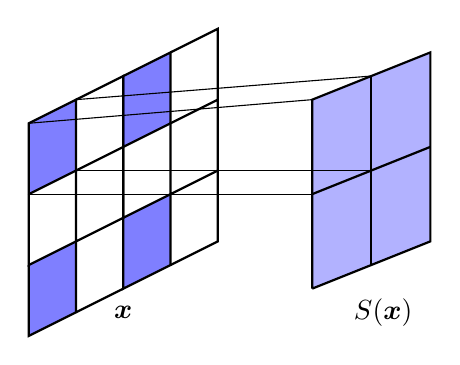
\begin{tikzpicture}[scale=0.6]
%\draw[opacity=0.5] (-4,-4) grid (4,4);

%%% grosse image

    % BLOCK (1,1)
% pixels bleu
\draw[thick, fill=blue, fill opacity=0.5] (-3,0) -- (-3,-1.5) -- (-4,-2)  -- (-4,-0.5);

% pixels blancs
\draw[thick, xshift=1cm, yshift=0.5cm] (-4,-2) -- (-3,-1.5);


    % BLOCK (2,1)
% pixels bleu
\draw[thick, fill=blue, fill opacity=0.5, xshift=2cm, yshift=1cm] (-3,0) -- (-3,-1.5) -- (-4,-2)  -- (-4,-0.5);

% pixels blancs
\draw[thick, xshift=3cm, yshift=1.5cm] (-3,0) -- (-3,-1.5) -- (-4,-2);

    % BLOCK (1,2)
% pixels bleu
\draw[thick, fill=blue, fill opacity=0.5, yshift=3cm] (-4,-2) -- (-4,-0.5) -- (-3,0) -- (-3,-1.5) -- (-4,-2);

% pixels blancs
\draw[thick, yshift=1.5cm] (-4,-0.5) -- (-4,-2) -- (-3,-1.5);
\draw[thick, xshift=1cm, yshift=3.5cm] (-4,-0.5) -- (-3,0) -- (-3,-1.5);

%pixels rouge
\draw[thick, xshift=1cm, yshift=2cm] (-4,-2) -- (-4,-0.5) -- (-3,0) -- (-3,-1.5) -- (-4,-2);

    % BLOCK (2,2)
% pixels bleu
\draw[thick, fill=blue, fill opacity=0.5, xshift=2cm, yshift=4cm] (-4,-2) -- (-4,-0.5) -- (-3,0) -- (-3,-1.5) -- (-4,-2);

% pixels blancs
\draw[thick, xshift=2cm, yshift=2.5cm] (-4,-0.5) -- (-4,-2) -- (-3,-1.5);
\draw[thick, xshift=3cm, yshift=4.5cm] (-4,-0.5) -- (-3,0) -- (-3,-1.5);

%pixels rouge
\draw[thick, xshift=3cm, yshift=3cm] (-4,-2) -- (-4,-0.5) -- (-3,0) -- (-3,-1.5) -- (-4,-2);

%%% petite image

\draw[thick, fill=blue, fill opacity=0.3, xshift=1cm] (1,-1) -- (1,3) -- (3.5,4) -- (3.5,0) -- (1,-1);
\draw[thick, xshift=2.25cm, yshift=0.5cm] (1,-1) -- (1,3);
\draw[thick, xshift=1cm, yshift=-2cm] (1,3) -- (3.5,4);

%%% lien

\draw (-4,1) -- (2,1);
\draw (-4,2.5) -- (2,3);
\draw (-3,1.5) -- (3.25,1.5);
\draw (-3,3) -- (3.25,3.5);

%%% Nom

\draw  (-2,-1.5) -- (-2,-1.5) node{$\bf{x}$};
\draw  (3.5,-1.5) -- (3.5,-1.5) node{$S(\bf{x})$};
\end{tikzpicture}
		}
	\end{floatrow}
\end{figure}

\begin{figure}[h]\centering
	\setlength{\tabcolsep}{5pt}
\begin{tabular}{c c c c c}

\ Sans  &  $\sigma=0.5$  &  $\sigma=0.6$  &  $a=0.6$  &  $a=0.4$

\\

\rotatebox[origin=lt]{90}{{\color{white}bb}filtre}


\includegraphics[width=0.14\textwidth]{resultats/compare_filter/seed21-f-filtre=s.png}
&

\includegraphics[width=0.14\textwidth]{resultats/compare_filter/seed21-f-filtre=g_param=0.5.png}
&

\includegraphics[width=0.14\textwidth]{resultats/compare_filter/seed21-f-filtre=g_param=0.6.png}
&

\includegraphics[width=0.14\textwidth]{resultats/compare_filter/seed21-f-filtre=p_param=0.6.png}
&

\includegraphics[width=0.14\textwidth]{resultats/compare_filter/seed21-f-filtre=p_param=0.4.png}

\\

\rotatebox[origin=lb]{90}{{\color{white}b}image $\bf{x}$}


\includegraphics[width=0.14\textwidth]{resultats/compare_filter/seed21-x.png}
&

\includegraphics[width=0.14\textwidth]{resultats/compare_filter/seed21-x.png}
&

\includegraphics[width=0.14\textwidth]{resultats/compare_filter/seed21-x.png}
&

\includegraphics[width=0.14\textwidth]{resultats/compare_filter/seed21-x.png}
&

\includegraphics[width=0.14\textwidth]{resultats/compare_filter/seed21-x.png}

\\

\rotatebox[origin=lb]{90}{{\color{white}l}mesure $A\bf{x}$}


\includegraphics[width=0.14\textwidth]{resultats/compare_filter/seed21-Ax-filtre=s.png}
&

\includegraphics[width=0.14\textwidth]{resultats/compare_filter/seed21-Ax-filtre=g_param=0.5.png}
&

\includegraphics[width=0.14\textwidth]{resultats/compare_filter/seed21-Ax-filtre=g_param=0.6.png}
&

\includegraphics[width=0.14\textwidth]{resultats/compare_filter/seed21-Ax-filtre=p_param=0.6.png}
&

\includegraphics[width=0.14\textwidth]{resultats/compare_filter/seed21-Ax-filtre=p_param=0.6.png}
\end{tabular}
	\caption{Quelques exemples d'applications de $A$ à une même image en fonction des filtres. }
\end{figure}

\begin{enonce}[Problématique]
	On considère $\bf{x_0}\in\R^{n\times m}$ une image que l'on cherche à reconstruire et $\ \bf{y_0}:=A(\bf{x_0})\ $ sa version sous-échantillonnée. Une bonne reconstruction de $\bf{x_0}$ étant un minimiseur :
	\begin{equation}\label{eq:probleme}
		\bf{x^*}\in \argmin{\bf{x}\in\R^{n\times m}}\ F(\bf{x})\end{equation}\end{enonce}

Si pour le bien de l'étude $\bf{x_0}$ sera connu, il va de soit que le problème ne nécessite pas de le connaître \apriori.
\\
Aussi, la linéarité de $A$ assure la convexité de $F$ mais, bien évidemment, son caractère hautement non injectif (surtout pour $pq\lll nm$) fait qu'il existe tout un sous-espace affine de minimum globaux. D'où l'intérêt des deux méthodes étudiées pour ``choisir'' ce minimum.
\\

\begin{wrapfigure}{r}{0.4\textwidth}% vire le [16]
	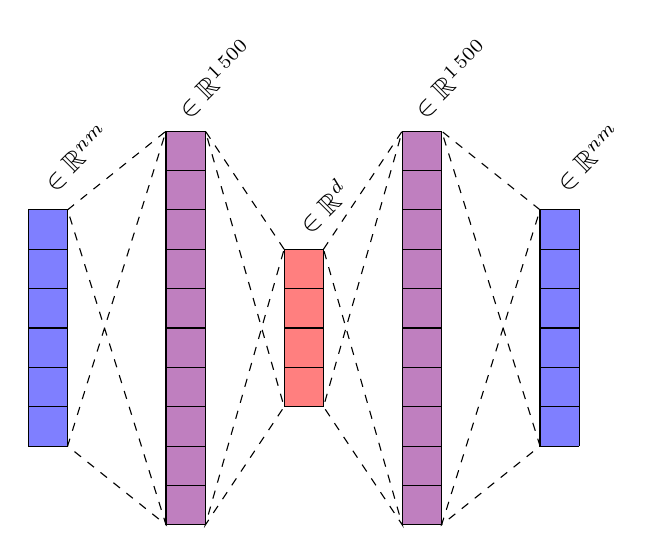
\begin{tikzpicture}[scale=0.5]
%\draw[thin, opacity=0.5] (-7.5,-6.5) grid (7.5,6.5);

%%% vecteurs

% input
\draw[fill=blue, fill opacity=0.5] (-7,-3) -- (-7,3) -- (-6,3)  -- (-6,-3) -- (-7,-3);
\draw (-7, 2) -- (-6, 2);
\draw (-7, 1) -- (-6, 1);
\draw (-7, 0) -- (-6, 0);
\draw (-7, -1) -- (-6, -1);
\draw (-7, -2) -- (-6, -2);

% hidden 1
\draw[fill=violet, fill opacity=0.5] (-3.5,-5) -- (-2.5,-5) -- (-2.5,5)  -- (-3.5,5) -- (-3.5,-5);
\draw (-3.5, 4) -- (-2.5, 4);
\draw (-3.5, 3) -- (-2.5, 3);
\draw (-3.5, 2) -- (-2.5, 2);
\draw (-3.5, 1) -- (-2.5, 1);
\draw (-3.5, 0) -- (-2.5, 0);
\draw (-3.5, -1) -- (-2.5, -1);
\draw (-3.5, -2) -- (-2.5, -2);
\draw (-3.5, -3) -- (-2.5, -3);
\draw (-3.5, -4) -- (-2.5, -4);

% latent
\draw[fill=red, fill opacity=0.5] (-0.5,-2) -- (0.5,-2) -- (0.5,2)  -- (-0.5,2) -- (-0.5,-2);
\draw (-0.5, 1) -- (0.5, 1);
\draw (-0.5, 0) -- (0.5, 0);
\draw (-0.5, -1) -- (0.5, -1);

% hidden 2
\draw[fill=violet, fill opacity=0.5] (3.5,-5) -- (2.5,-5) -- (2.5,5)  -- (3.5,5) -- (3.5,-5);
\draw (3.5, 4) -- (2.5, 4);
\draw (3.5, 3) -- (2.5, 3);
\draw (3.5, 2) -- (2.5, 2);
\draw (3.5, 1) -- (2.5, 1);
\draw (3.5, 0) -- (2.5, 0);
\draw (3.5, -1) -- (2.5, -1);
\draw (3.5, -2) -- (2.5, -2);
\draw (3.5, -3) -- (2.5, -3);
\draw (3.5, -4) -- (2.5, -4);

% output
\draw[fill=blue, fill opacity=0.5] (7,-3) -- (7,3) -- (6,3)  -- (6,-3) -- (7,-3);
\draw (7, 2) -- (6, 2);
\draw (7, 1) -- (6, 1);
\draw (7, 0) -- (6, 0);
\draw (7, -1) -- (6, -1);
\draw (7, -2) -- (6, -2);

%%% liens

\draw[dashed, thin] (-6,3) -- (-3.5,5) -- (-6,-3) -- (-3.5,-5) -- (-6,3);
\draw[dashed, thin] (-0.5,2) -- (-2.5,5) -- (-0.5,-2) -- (-2.5,-5) -- (-0.5,2);
\draw[dashed, thin] (0.5,2) -- (2.5,5) -- (0.5,-2) -- (2.5,-5) -- (0.5,2);
\draw[dashed, thin] (6,3) -- (3.5,5) -- (6,-3) -- (3.5,-5) -- (6,3);

%%% tailles

\draw (-5.75,4.25) -- (-5.75,4.25) node[]{\rotatebox[origin=lt]{45}{$\in\R^{nm}$}};
\draw (-2.25,6.25) -- (-2.25,6.25) node[]{\rotatebox[origin=lt]{45}{$\in\R^{1\,500}$}};
\draw (0.5,3) -- (0.5,3) node[]{\rotatebox[origin=lt]{45}{$\in\R^d$}};
\draw (3.75,6.25) -- (3.75,6.25) node[]{\rotatebox[origin=lt]{45}{$\in\R^{1\,500}$}};
\draw (7.25,4.25) -- (7.25,4.25) node[]{\rotatebox[origin=lt]{45}{$\in\R^{nm}$}};
\end{tikzpicture}
	\caption{Schéma des auto-encodeurs  $f$ avec $d=100,\ 200,\ 400,\ 800$}
	\label{fig:AEschem}
\end{wrapfigure}

Les auto-encodeurs utilisés pour paramétrer l'espace des images sont des réseaux MLP que l'on notera indifféremment $f$ et dont $f_E$ et $f_D$ sont les parties encodage et décodage :
\[f = f_E\circ f_D\]
Conformément à la figure \textit{\ref{fig:AEschem}}, ils se composent tous d'une couche cachée de taille $1\,500$ pour les parties encodeurs et décodeurs et la seule chose qui les différencie est la taille de leur espace latent qui varient entre $100$ et $800$. Leur entraînement s'est fait sur le jeu de données MNIST et c'est donc uniquement sur ces images que seront présentés les résultats. Plus de détails sur les performances des auto-encodeurs en annexe \ref{anx:AE}.
\\




\subsection{Cadre théorique de l'article}\label{sec:article1/2}

Comme expliqué plus tôt, tout l'objet de l'article \cite{traonmilin_basins_2022} est d'étudier dans quelle mesure il est possible de faire une descente de gradient sur une paramétrisation (non-convexe) d'un modèle plutôt que sur le modèle lui-même.
\\
Pour cela, on note $\Sigma\subset\R^{n\times m}$ le modèle de basse-dimension et $\phi: \R^d\lr\R^{n\times m}$ une paramétrisation de ce dernier avec :
\begin{align*}\Sigma&\subset\phi\big(\R^d\big)  &  \Theta&:=\phi^{-1}(\Sigma)\end{align*}
\\
La paramétrisation $\phi$, doit vérifier certaines hypothèses de régularité pour pouvoir appliquer les résultats de l'article. Dans notre cas, $\ \phi=f_D\ $ dont les fonctions d'activations sont toutes des sigmoïdes. Elle est donc $C^{\infty}$ et pour cette raison on ne s'attardera pas outre mesure sur les questions de régularité de $\phi$.
\\

\textit{\`A noter qu'on ne suppose ni que $\ \phi(\R^d)=\Sigma\ $ ni que  $\ \Theta=\R^d$ et ce ne sera pas le cas pour nous. Aussi, le formalisme proposé par Traonmilin \etal est légèrement différent de celui donné en section précédente. Il y est considéré un espace de mesure $\mathcal{D}$ et les signaux (dans notre cas les images) sont pris dans $\mathcal{D}^*$, de sorte que la mesure par $\alpha\in\mathcal{D}$ de $x\in\mathcal{D}^*$ soit représentéé par le crochet de dualité $\langle \alpha,x\rangle$. Cela à son intérêt surtout en dimension infinie, mais autrement, cette écriture est tout à fait équivalente à celle donnée en section \ref{sec:forma2pb}}
\\

\begin{wrapfigure}{r}{0.43\textwidth}
	\fbox{\begin{minipage}{15em}
\vspace{0.3cm}
\begin{algorithmic}[0]
    \State $\theta_0$ : initialisation
    \State $x$ : image à reconstruire
    \State $\tau$ : pas de descente
    \State $N$ : nombre d'itération
    \State $\hat{x}\ \longleftarrow\ f(x)$
    \State
    \For{$n\in \llbracket1,N-1\rrbracket$}
        \State $\theta_{n+1}\ \longleftarrow\ \theta_n\ - \tau \nabla g(\theta_un)$
        \State $x_{n+1}\ \longleftarrow\ f_D(\theta_{n+1})$
        \EndFor
    \State
    \Return $(x_n)_{0\leq n\leq N}$
\end{algorithmic}
\vspace{0.2cm}
\end{minipage}}
	\caption{Algorithme de descente depuis l'espace des paramètres}
	\label{fig:pcode LGD}
\end{wrapfigure}

Le problème est donc de trouver les paramètres $\theta^*$ minimisant $\ g:=A\phi\ $ sur $\Theta$, ou dans notre cas :
\[\theta^*\in\argmin{\theta\in\Theta}\ \frac{1}{2}{\big\|Af_D(\theta)-\bf{y_0}\big\|_2}^2\]
\\
Minimum que l'on cherche à obtenir par descente de gradient. On considérera donc dans toute la suite, $(\theta_n)$ la descente de gradient à pas fixe, $\forall\theta_0\in\R^d$ :
\[\forall n\in\N^*,\qquad \theta_{n+1} = \theta_n - \tau\nabla g(\theta_n)\]
Sachant que $\phi$ est n'est pas convexe, on introduit la définition suivante :
\\ \\
\begin{definition}
	Une partie $\Lambda\subset\Theta$ de $\R^d$ sera un \emph{bassin d'attraction} de minimum global $\theta^*\in\Lambda$ si en tout point $\theta_0\in\Lambda$, alors existe un pas de descente $\tau_0$ tel que :
	\[\forall \tau\in]0,\tau_0],\qquad \lim_{n\lr+\infty}g\big(\theta_n\big)=g(\theta^*)\]
\end{definition}

Avec cette définition, $(\theta_n)$ peut tout à fait converger vers un autre minimum que $\theta^*$. Pour en tenir compte en même temps que la potentielle non-injectivité de $\phi$, ils introduisent les définitions suivantes :
\\
\begin{definition}\label{def:boule}
	On note $d(\theta,\theta^*)$ la distance de $\theta$ au plus proche paramètre de même image de $\theta^*$ et $p(\theta,\theta^*)$ la projection (potentiellement multivaluée) de $\theta$ sur ce même paramètre, e.i. sur $\phi^{-1}\circ\phi(\{\theta^*\})$ :
	$\forall\theta\in\R^d$ :
	\begin{align*}d(\theta,\theta^*) &:=\min_{\substack{\Tilde{\theta}\in\Theta\\ \phi(\Tilde{\theta})=\phi(\theta^*)}}\ \big\|\Tilde{\theta}-\theta\big\|_2  &  p(\theta,\theta^*)&:=\argmin{\substack{\Tilde{\theta}\in\Theta\\ \phi(\Tilde{\theta})=\phi(\theta^*)}}\ \big\|\Tilde{\theta}-\theta\big\|_2\subset\R^d\end{align*}
	Avec, sont définis les bassins $\Lambda_\beta(\theta^*)$ de la forme :
	\[\forall \beta\in\R^{+_*},\qquad \Lambda_\beta(\theta^*):=\big\{\theta\in\R^d\ |\ d(\theta, \theta^*)<\beta\big\}\]
\end{definition}

Contrairement aux exemples traités dans l'article, la paramétrisation par l'espace latent ne donne pas de formule vraiment exploitable pour $\phi=f_D$. En revanche, $f_D$ faisant parti d'un auto-encodeur, on peut supposer que $f_E$ est la réciproque de $f_D$ au moins sur $\Theta$ :
\begin{align*} {{f_{D}}_{\displaystyle |_{\Theta}}}^{-1}&={f_{E}}_{\displaystyle |_{\Sigma}}  & &\text{avec} & \Theta&=f_E(\Sigma)
\end{align*}
\\
En particulier, cela permet d'avoir l'injectivité de $f_D$ sur $\Theta$. Ce dont il découle que $d(\theta,\theta^*)=\|\theta-\theta^*\|_2$ est une distance (ce qui n'est pas le cas en général), que $\Lambda_\beta(\theta^*)$ une boule ouverte et que $\ p(\theta,\theta^*)=\theta^*$.

\emph{Cette hypothèse est quand-même très forte, elle sera détaillé dans la section \ref{sec:PGD}}
\\

Enfin, dans toute la suite $\Sigma$ sera supposé être un cône, c'est-à-dire que pour tout $\lambda>0$, $\lambda\Sigma=\Sigma\ $ et sont introduits les deux ensembles suivants :
\\

\begin{definition} On appelle \emph{ensemble des sécantes de $\Sigma$} l'ensemble :
	\[\mathcal{S}(\Sigma) := \Sigma-\Sigma = \big\{x-y\in\R^{n\times m}\ |\ x,y\in\Sigma\big\}\]
	\\
	En notant $\partial_u\phi(\theta)$ la dérivée directionnelle de $\phi$ en $\theta$ et dans la direction $u$, on définit l'\emph{ensemble généralisé des sécantes de $\Sigma$}, l'ensemble noté :
	\[\overline{\mathcal{S}(\Sigma)}:=\mathcal{S}(\Sigma)\cup\Big\{\partial_u\phi(\theta)\ |\ \forall (\theta,u)\in\Theta\times\R^d\Big\}\]{\color{white}l}
	
	\emph{Pour nous, $\phi=f_D\ $ est $C^\infty$, donc la dérivée directionnelle $\partial_u\phi(u)$ est équivalente à la différentielle de $\phi$ au point $\theta$ valué en $u$, $D_\theta\phi(u)$.}
\end{definition}

L'auto-encodeur $f$ n'a été entraîné que sur des images dont les pixels prennent valeur dans $[0,1]$ et il n'est capable de reconstruire que ce type d'image. Et ce, pour la simple et bonne raison que ses fonctions d'activation sont des sigmoïdes y compris celles de sortie. Il est donc strictement impossible qu'une image $f_D(\theta)$ prenne des valeurs au-delà de 1, ce qui va à l'encontre de l'hypothèse que $\Sigma$ soit un cône.
\\
Si ce choix de fonction d'activation a été fait c'était à l'origine pour reprendre les codes de l'article \cite{peng_solving_2019} sur la descente projetée (voir section \ref{sec:comparPGD}), mais en toute vraisemblance utiliser des fonctions ReLu ou autre ne devrait pas trop changer les résultats obtenus.
La perte de régularité entraînée ne devrait pas non plus être un problème en pratique et pourrait rendre l'hypothèse un peu plus raisonnable.
\\




\subsection{Les résultats de Traonmilin {\itshape et al.}}\label{sec:article2/2}

Le théorème de Traonmilin \etal, dans le cas sans bruit, s'énonce ainsi :
\\
\begin{theoreme}[sans bruit]\label{theo:maintheo} Soit $\theta^*\in\Theta$ un minimiseur global de $g$. Si on a les hypothèses suivantes :
	\begin{itemize}
		\item l'opérateur de mesure $A$ est continue et vérifie la \emph{propriété d'isométrie restreinte} (RIP) de constante $\gamma\in]0,1]$ :
		\begin{equation}\label{eq:RIP}
			\forall v\in\overline{\mathcal{S}(\Sigma)},\qquad (1-\gamma)\|v\|^2\leq \|Av\|^2\leq (1+\gamma)\|v\|^2
		\end{equation}
		
		\item Si $\Lambda_{2\beta}(\theta^*)$, tel que défini en \ref{def:boule}, est inclus dans $\Theta$, ou autrement dit :
		\begin{equation}\label{eq:LambinTheta}
			\phi\big(\Lambda_{2\beta}\big)\subset\Sigma
		\end{equation}
		
		\item Si la \emph{technical assumption} \ref{hyp:technical} (donnée plus bas) est vérifiée sur $\Lambda_{2\beta}$ avec la constante $C>0$ et qu'il existe $\Tilde{\theta}\in p(\theta,\theta^*)$ tel qu'on ait l'inégalité :
		\begin{equation}\label{eq:majo3}
			\forall z\in[\theta,\Tilde{\theta}],\qquad \frac{(1-\gamma){\big\|\partial_{\Tilde{\theta}-\theta}\phi(z)\big\|_2}^2}{\sqrt{1+\gamma}\big\|A\partial^2_{\Tilde{\theta}-\theta}\phi(z)\big\|_2}\geq C\beta
		\end{equation}
	\end{itemize}
	
	Si $A$ et $\phi$ vérifient de plus la \emph{framework assumption} \ref{hyp:framework}, alors l'ensemble $\Lambda_\beta(\theta^*)$ est un bassin d'attraction.  
\end{theoreme}

\begin{corollaire}
	En particulier, s'il existe une constante $\beta_1>0$ vérifiant la \emph{technical assumption} \ref{hyp:technical} et telle que $p(\,\cdot\,, \theta^*)$ soit mono-valuée sur $\Lambda_{\beta_1}(\theta^*)$ :
	\[\forall \theta\in\Lambda_{\beta_1}(\theta^*),\qquad p(\theta,\theta^*)=\big\{\Tilde{\theta}\big\}\]
	\\
	Alors $\Lambda_{\min(\beta_1,\beta_2)}(\theta^*)$ est un bassin d'attraction, où $\beta_2$ est donné par la formule :
	\[\beta_2:=\frac{1-\gamma}{C\sqrt{1+\gamma}}\inf_{\theta\in\Lambda_{\beta_1}(\theta^*)}\inf_{z\in[\theta,\Tilde{\theta}]}\frac{{\big\|\partial_{\Tilde{\theta}-\theta}\phi(z)\big\|_2}^2}{\big\|A\partial^2_{\Tilde{\theta}-\theta}\phi(z)\big\|_2}\]
\end{corollaire}

Ce théorème (et son corollaire) donne une estimation de la marge que l'on a autour de $\theta^*$ pour initialiser la descente de gradient depuis l'espace des paramètres de sorte à s'assurer sa convergence. En particulier, l'inégalité \ref{eq:majo3} donne, sachant $\gamma$ et $C$, à quel point le ``rayon'' du bassin $\beta$ peut être grand.
Estimation qui est donc valable sachant les deux hypothèses supplémentaires :
\\
\begin{assump}[Technical assumption]\label{hyp:technical}
	La \emph{technical assumption} est vérifiée sur $\Lambda_{2\beta}(\theta^*)$ avec la constante $C>0$ si elle donne un contrôle de $d$ sur $\|\cdot\|_2$ :
	\[\forall\theta\in\Lambda_{2\beta}(\theta^*),\qquad \big\|\theta-\theta^*\big\|_2\leq C d\big(\theta, \theta^*\big)\]
	et si les deux premières dérivées (directionnelles) de $A\phi$ sont uniformément bornées respectivement sur $\phi^{-1}\circ\phi(\{\theta^*\})$ et $\Lambda_{2\beta}$ :
	\begin{align*}\sup_{\theta\in\phi^{-1}\circ\phi(\{\theta^*\})}\sup_{\|u\|_2=1}\big\|A\partial_u\phi(\theta)\big\|_2&<+\infty  &  \sup_{\theta\in\Lambda_{2\beta}(\theta^*)}\sup_{\|u\|_2,\|v\|_2=1}\big\|A\partial_u\partial_v\phi(\theta)\big\|_2&<+\infty
	\end{align*}
\end{assump}

Comme dit plus haut, supposer $\phi=f_D$ inversible sur $\Theta$ impose $\ d\big(\theta, \theta^*\big)=\big\|\theta-\theta^*\big\|_2$. Ainsi la première inégalité est vérifiée pour tout $C\geq1$ et les majorations uniformes ne sont pas un problème non plus puisque $f_D$ est $C^\infty$. Sachant que c'est l'inégalité \ref{eq:majo3} qui nous intéresse, on va plutôt avoir tendance à prendre $C=1$.
\\

\begin{assump}[Framework assumption]\label{hyp:framework}
	La paramétrisation $\phi$ doit être deux fois (Gateaux) différentiable et il faut que pour toute suite $|h_n|\xrightarrow[n\lr+\infty]{} 0$, $\left\|\frac{\phi(\theta +|h_n|v)-\phi(\theta)}{|h_n|}\right\|_2$ converge indépendant de $(|h_n|)$ et ceux, pour tout $(\theta,v)$ tel que $\partial_v\phi(\theta)\in\overline{\mathcal{S}(\Sigma)}$.
\end{assump}

Dans l'article \cite{traonmilin_basins_2022}, la mesure de proximité des images est faite à travers une norme $\|\cdot\|_\mathcal{H}$ associé un espace hilbertien $\mathcal{H}$ contenant $\Sigma$. Cette hypothèse permet alors de s'assurer que cette norme s'étende à $\overline{\mathcal{S}(\Sigma})$. Mais encore, une fois, pour nous $\mathcal{H}=\R^{n\times m}$ et il n'y a pas de risque à ce sujet. Aussi, le fait que $\phi=f_E$ soit différentiable rend immédiat la convergence de la suite $\left\|\frac{\phi(\theta +|h_n|v)-\phi(\theta)}{|h_n|}\right\|_2$ indépendamment de $\big(|h_n|\big)_n$.
\\ \\

Revenons maintenant aux autres hypothèses du théorème.
\\
D'abord, dans la RIP (\ref{eq:RIP}), c'est surtout l'inégalité de gauche qui est importante puisqu'elle garantit que $A$ soit inversible sur $\overline{\mathcal{S}(\Sigma)}$.
\\
Comme $\Sigma$ n'est pas proprement définie, le mieux qu'on puisse faire c'est de vérifier si c'est au moins le cas pour tous les $\bf{x}-\bf{y}$ avec $\bf{x}$, $\bf{y}$ du jeu de données (MNIST donc). Pour se faire, on les équivalences :
\begin{align*}(1-\gamma)\|v\|^2\leq \|Av\|^2\leq (1+\gamma)\|v\|^2\ &\Llr\ \frac{\|Av\|^2}{\|v\|^2}-1\leq \gamma\\
	&\Llr\ \left|\frac{\|Av\|^2}{\|v\|^2}-1\right|\leq \gamma\end{align*}
En calculant le rapport $\left|\frac{\|Av\|^2}{\|v\|^2}-1\right|$, on peut donc estimer une borne pour $\gamma$. Seulement, avec les moyens disponibles et notre code, passer en revue les $60\,000\times(60\,000+1)$ couples d'images du set de test demanderait quelque $11$h de calcul. On se contentera donc, faute de mieux, de faire les calculs sur $\Sigma$, ce qui nous donnes les histogrammes \textit{\ref{fig:RIP-s}} et \textit{\ref{fig:RIP-g}} :
\\

\begin{figure}[h]
	\begin{floatrow}
		\ffigbox{\caption{Histogramme des valeurs de $\big|{\|Av\|_2}^2/{\|v\|_2}^2-1\big|$ sans filtre passe-bas sur le set de test}\label{fig:RIP-s}}
		{% This file was created with tikzplotlib v0.10.1.
\begin{tikzpicture}

\definecolor{darkgray176}{RGB}{176,176,176}
\definecolor{steelblue31119180}{RGB}{31,119,180}

\begin{axis}[
height=\figheight,
tick align=outside,
tick pos=left,
width=\figwidth,
x grid style={darkgray176},
xmin=0.567671617865562, xmax=0.894375541806221,
xtick style={color=black},
y grid style={darkgray176},
ymin=-72.35, ymax=1519.35,
ytick style={color=black}
]
\addplot [semithick, steelblue31119180]
table {%
0.582521796226501 1
0.583117008209229 0
0.596806526184082 0
0.597401738166809 1
0.597996950149536 0
0.605139255523682 0
0.605734586715698 1
0.606329679489136 0
0.614067316055298 0
0.614662408828735 1
0.615257740020752 0
0.615852832794189 0
0.616448044776917 1
0.617043256759644 1
0.617638468742371 0
0.62597119808197 0
0.626566410064697 1
0.627161622047424 1
0.627756834030151 2
0.628351926803589 0
0.63013768196106 0
0.630732774734497 1
0.631327986717224 1
0.631923198699951 0
0.639065504074097 0
0.640255928039551 2
0.640851140022278 0
0.642041563987732 0
0.642636775970459 1
0.643231868743896 0
0.643827199935913 0
0.644422292709351 1
0.645017623901367 1
0.645612716674805 0
0.650969505310059 0
0.651564717292786 1
0.652159929275513 0
0.65275502204895 0
0.653350353240967 2
0.653945446014404 1
0.654540777206421 1
0.655135869979858 0
0.655731081962585 0
0.656326293945312 1
0.65692150592804 1
0.657516717910767 0
0.658111810684204 0
0.658707141876221 3
0.659302234649658 0
0.659897565841675 3
0.661087870597839 1
0.661683082580566 2
0.662278294563293 1
0.662873506546021 2
0.663468599319458 0
0.664063930511475 1
0.664659023284912 0
0.665254235267639 2
0.665849447250366 2
0.66703987121582 0
0.667634963989258 0
0.668825387954712 2
0.669420719146729 1
0.670611023902893 1
0.67120623588562 0
0.671801447868347 0
0.672396659851074 2
0.673587083816528 0
0.674182176589966 2
0.674777388572693 2
0.67537260055542 1
0.677753448486328 1
0.678943872451782 3
0.67953896522522 1
0.680134177207947 0
0.680729389190674 2
0.681324601173401 1
0.682514905929565 1
0.683110237121582 3
0.68370532989502 1
0.684300661087036 3
0.684895753860474 1
0.685490965843201 1
0.686086177825928 3
0.686681389808655 2
0.688467025756836 5
0.689062118530273 1
0.689657330513 7
0.690252542495728 2
0.690847754478455 2
0.691442966461182 4
0.692038059234619 4
0.692633390426636 7
0.693228483200073 2
0.69382381439209 3
0.694418907165527 6
0.695014119148254 5
0.695609331130981 8
0.696204543113708 3
0.696799755096436 3
0.697394847869873 4
0.69799017906189 3
0.698585271835327 11
0.699180603027344 5
0.699775695800781 7
0.700370907783508 10
0.701561331748962 6
0.702156543731689 7
0.702751636505127 6
0.703346967697144 14
0.703942060470581 7
0.705132484436035 11
0.705727696418762 11
0.706322908401489 7
0.706918001174927 20
0.707513332366943 14
0.708108425140381 22
0.708703756332397 16
0.709298849105835 17
0.709894061088562 15
0.710489273071289 22
0.711084485054016 16
0.711679697036743 24
0.712274789810181 25
0.712870121002197 30
0.713465213775635 19
0.714060544967651 37
0.714655637741089 27
0.715250849723816 22
0.715846061706543 34
0.71644127368927 43
0.717036485671997 37
0.717631578445435 54
0.718226909637451 38
0.718822002410889 59
0.719417214393616 50
0.720012426376343 57
0.72060763835907 70
0.721202850341797 78
0.721797943115234 59
0.722393274307251 66
0.722988367080688 82
0.723583698272705 79
0.724178791046143 111
0.72477400302887 121
0.725369215011597 119
0.725964426994324 139
0.726559638977051 117
0.727154731750488 150
0.727750062942505 191
0.728345155715942 178
0.728940367698669 186
0.729535579681396 188
0.730130791664124 181
0.730726003646851 237
0.731321215629578 267
0.731916427612305 285
0.732511520385742 313
0.733106851577759 346
0.733701944351196 346
0.734297156333923 425
0.73489236831665 414
0.736082792282104 506
0.736677885055542 518
0.737273216247559 549
0.737868309020996 628
0.738463640213013 638
0.73905873298645 706
0.739653944969177 834
0.740249156951904 809
0.740844368934631 860
0.741439580917358 876
0.742034673690796 973
0.742630004882812 1026
0.74322509765625 1049
0.744415521621704 1171
0.745010733604431 1191
0.745605945587158 1260
0.746201038360596 1277
0.746796369552612 1324
0.74739146232605 1358
0.747986793518066 1408
0.748581886291504 1335
0.749177098274231 1405
0.749772310256958 1425
0.750367522239685 1371
0.750962734222412 1388
0.75155782699585 1447
0.752153158187866 1335
0.752748250961304 1311
0.75334358215332 1327
0.753938674926758 1198
0.754533886909485 1276
0.755129098892212 1223
0.755724310874939 1151
0.756319522857666 1134
0.756914615631104 1017
0.75750994682312 1047
0.758105039596558 934
0.759295463562012 850
0.759890675544739 735
0.760485887527466 751
0.761080980300903 635
0.76167631149292 631
0.762271404266357 566
0.762866735458374 542
0.763461828231812 527
0.764057040214539 466
0.764652252197266 455
0.765247464179993 467
0.76584267616272 350
0.766437768936157 312
0.767033100128174 314
0.767628192901611 252
0.768223404884338 237
0.768818616867065 258
0.769413828849792 227
0.77000904083252 206
0.770604252815247 190
0.771199464797974 184
0.772389888763428 112
0.772984981536865 142
0.773580193519592 143
0.774175405502319 133
0.774770617485046 97
0.775365829467773 118
0.775960922241211 94
0.776556253433228 84
0.777151346206665 81
0.777746677398682 86
0.778341770172119 70
0.778936982154846 61
0.779532194137573 54
0.7801274061203 60
0.780722618103027 50
0.781317710876465 51
0.781913042068481 39
0.782508134841919 30
0.783103346824646 40
0.783698558807373 48
0.7842937707901 28
0.784888982772827 28
0.785484075546265 29
0.786079406738281 31
0.786674499511719 29
0.787269830703735 16
0.7884601354599 30
0.789650559425354 22
0.790245771408081 13
0.790840864181519 27
0.791436195373535 18
0.792031288146973 18
0.792626619338989 20
0.793221712112427 13
0.793816924095154 10
0.794412136077881 14
0.795007348060608 15
0.795602560043335 8
0.796197652816772 17
0.796792984008789 6
0.797388076782227 11
0.797983288764954 11
0.798578500747681 9
0.799173712730408 8
0.799768924713135 8
0.800364017486572 3
0.800959348678589 5
0.801554441452026 3
0.802149772644043 4
0.80274486541748 3
0.803340077400208 5
0.803935289382935 9
0.804530501365662 5
0.805720806121826 7
0.806316137313843 9
0.80691123008728 3
0.807506561279297 3
0.808696866035461 1
0.809292078018188 1
0.809887290000916 3
0.810482501983643 2
0.81107759475708 5
0.812268018722534 1
0.812863230705261 3
0.813458442687988 0
0.814053654670715 6
0.814648866653442 4
0.81524395942688 1
0.815839290618896 2
0.816434383392334 1
0.817029714584351 2
0.817624807357788 2
0.818220019340515 3
0.818815231323242 3
0.819410443305969 0
0.820005655288696 2
0.820600748062134 0
0.82119607925415 3
0.821791172027588 3
0.822386384010315 2
0.822981595993042 0
0.823576807975769 0
0.824172019958496 1
0.824767231941223 0
0.82536244392395 3
0.825957536697388 2
0.826552867889404 0
0.827147960662842 2
0.828338384628296 0
0.828933596611023 1
0.82952880859375 0
0.830719232559204 0
0.831314325332642 1
0.831909656524658 0
0.833099961280823 0
0.83369517326355 1
0.834290385246277 0
0.834885597229004 1
0.835480690002441 0
0.839647054672241 0
0.840242385864258 1
0.840837478637695 1
0.841432809829712 0
0.843813538551331 0
0.844408750534058 1
0.845003843307495 0
0.845599174499512 1
0.846194267272949 0
0.863455057144165 0
0.864050269126892 1
0.864645481109619 0
0.870597362518311 0
0.871192693710327 1
0.871787786483765 0
0.87893009185791 0
0.879525423049927 2
};
\end{axis}

\end{tikzpicture}

		}
		
		\ffigbox{\caption{Histogramme des valeurs de $\big|{\|Av\|_2}^2/{\|v\|_2}^2-1\big|$ avec filtre gaussien ($\sigma=0,6$) sur le set de test}\label{fig:RIP-g}}
		{% This file was created with tikzplotlib v0.10.1.
\begin{tikzpicture}

\definecolor{darkgray176}{RGB}{176,176,176}
\definecolor{steelblue31119180}{RGB}{31,119,180}

\begin{axis}[
height=\figheight,
tick align=outside,
tick pos=left,
width=\figwidth,
x grid style={darkgray176},
xmin=0.765329128503799, xmax=0.902652496099472,
xtick style={color=black},
y grid style={darkgray176},
ymin=-20.25, ymax=425.25,
ytick style={color=black}
]
\addplot [semithick, steelblue31119180]
table {%
0.771571159362793 1
0.771821260452271 1
0.772071480751038 0
0.772822022438049 0
0.773072242736816 1
0.773322343826294 0
0.773822784423828 0
0.774072885513306 1
0.774322986602783 0
0.77457332611084 2
0.774823427200317 0
0.775073528289795 3
0.775323867797852 1
0.775573968887329 0
0.775824069976807 0
0.776074409484863 2
0.776324510574341 1
0.777075052261353 1
0.777575373649597 3
0.777825593948364 1
0.778075695037842 0
0.778325915336609 3
0.778576135635376 1
0.778826236724854 4
0.779326677322388 4
0.779576778411865 1
0.779826998710632 3
0.780077219009399 3
0.780327320098877 0
0.780577540397644 2
0.781328082084656 5
0.781578302383423 5
0.7818284034729 2
0.782078623771667 9
0.782328844070435 6
0.782578945159912 8
0.782829165458679 8
0.783079385757446 7
0.783329486846924 9
0.783579707145691 4
0.783829927444458 14
0.784080028533936 10
0.784330248832703 13
0.78458046913147 7
0.784830570220947 16
0.785080790519714 10
0.785331010818481 21
0.785581111907959 12
0.785831332206726 15
0.786081552505493 13
0.786331653594971 15
0.786581873893738 7
0.786832094192505 14
0.787082195281982 14
0.78733241558075 15
0.787582635879517 17
0.787832736968994 22
0.788082838058472 18
0.788333177566528 17
0.788583278656006 21
0.788833379745483 38
0.78908371925354 26
0.789333820343018 31
0.789583921432495 24
0.789834260940552 24
0.790084362030029 40
0.790334463119507 44
0.790584802627563 44
0.790834903717041 31
0.791085004806519 36
0.791335225105286 44
0.791585445404053 44
0.79183554649353 48
0.792085766792297 46
0.792335987091064 51
0.792586088180542 47
0.793086528778076 51
0.793336629867554 73
0.793586850166321 64
0.793837070465088 68
0.794087171554565 54
0.794337391853333 52
0.7945876121521 84
0.794837713241577 76
0.795087933540344 72
0.795338153839111 72
0.795588254928589 79
0.795838475227356 71
0.796088695526123 107
0.796338796615601 88
0.796589016914368 96
0.796839237213135 89
0.797089338302612 94
0.797339558601379 100
0.797589778900146 100
0.797839879989624 84
0.798090100288391 96
0.798340320587158 100
0.798590421676636 94
0.798840641975403 107
0.79909086227417 110
0.799340963363647 126
0.799591183662415 124
0.799841403961182 107
0.800091505050659 132
0.800341725349426 121
0.800591945648193 122
0.800842046737671 138
0.801092267036438 149
0.801342487335205 129
0.801592588424683 150
0.80184280872345 159
0.802093029022217 151
0.802343130111694 156
0.802593231201172 159
0.802843570709229 176
0.803093671798706 144
0.803343772888184 140
0.80359411239624 178
0.803844213485718 174
0.804094314575195 169
0.804344654083252 183
0.804594755172729 192
0.804844856262207 182
0.805095195770264 188
0.805345296859741 162
0.805595397949219 172
0.805845618247986 174
0.806095838546753 215
0.80634593963623 197
0.806596159934998 189
0.806846380233765 220
0.807096481323242 240
0.807346701622009 199
0.807596921920776 198
0.807847023010254 226
0.808097243309021 199
0.808347463607788 234
0.808597564697266 235
0.8090980052948 213
0.809348106384277 222
0.809598326683044 244
0.809848546981812 244
0.810098648071289 264
0.810348868370056 232
0.810599088668823 266
0.810849189758301 256
0.811099410057068 284
0.811349630355835 261
0.811599731445312 286
0.81184995174408 286
0.812100172042847 255
0.812350273132324 267
0.812600493431091 300
0.812850713729858 267
0.813100814819336 301
0.813351035118103 298
0.81360125541687 265
0.813851356506348 259
0.814101576805115 278
0.814351797103882 311
0.814601898193359 317
0.814852118492126 298
0.815102338790894 291
0.815352439880371 298
0.815602660179138 344
0.815852880477905 305
0.816102981567383 304
0.81635308265686 298
0.816603422164917 300
0.816853523254395 321
0.817103624343872 282
0.817353963851929 271
0.817604064941406 341
0.817854166030884 310
0.81810450553894 323
0.818354606628418 303
0.818604707717896 333
0.818855047225952 331
0.81910514831543 343
0.819355249404907 362
0.819605588912964 330
0.819855690002441 353
0.820105791091919 342
0.820356011390686 338
0.820606231689453 331
0.820856332778931 331
0.821106553077698 319
0.821356773376465 323
0.821606874465942 345
0.821857094764709 381
0.822107315063477 328
0.822357416152954 341
0.822607636451721 331
0.822857856750488 331
0.823107957839966 405
0.823358178138733 352
0.8236083984375 337
0.823858499526978 349
0.824108719825745 357
0.824358940124512 342
0.824609041213989 284
0.824859261512756 351
0.825109481811523 333
0.825359582901001 344
0.825609803199768 324
0.825860023498535 327
0.826110124588013 344
0.82636034488678 290
0.826610565185547 334
0.826860666275024 331
0.827110886573792 331
0.827361106872559 351
0.827611207962036 350
0.827861428260803 348
0.82811164855957 336
0.828361749649048 305
0.828611969947815 341
0.828862190246582 307
0.82911229133606 334
0.829362511634827 326
0.829612731933594 302
0.829862833023071 310
0.830113053321838 303
0.830363273620605 298
0.830613374710083 278
0.830863475799561 299
0.831113815307617 351
0.831363916397095 290
0.831614017486572 276
0.831864356994629 293
0.832114458084106 300
0.832364559173584 313
0.832614898681641 307
0.832864999771118 291
0.833115100860596 310
0.833365440368652 286
0.83361554145813 284
0.833865642547607 307
0.834115862846375 308
0.834366083145142 297
0.834616184234619 295
0.834866404533386 274
0.835116624832153 297
0.835366725921631 290
0.835616946220398 258
0.835867166519165 290
0.836117267608643 259
0.83636748790741 274
0.836617708206177 254
0.836867809295654 241
0.837118029594421 240
0.837368249893188 285
0.837618350982666 237
0.837868571281433 273
0.8381187915802 252
0.838368892669678 246
0.838619112968445 224
0.838869333267212 239
0.839119434356689 232
0.839369654655457 242
0.839619874954224 211
0.839869976043701 248
0.840120196342468 220
0.840370416641235 187
0.840620517730713 233
0.84087073802948 234
0.841120958328247 218
0.841371059417725 223
0.841621279716492 219
0.841871500015259 217
0.842121601104736 226
0.842371821403503 217
0.842622041702271 210
0.842872142791748 199
0.843122363090515 206
0.843372583389282 185
0.84362268447876 188
0.843872904777527 173
0.844123125076294 186
0.844373226165771 219
0.844623446464539 191
0.844873666763306 171
0.845123767852783 169
0.845373868942261 160
0.845624208450317 206
0.845874309539795 159
0.846124410629272 185
0.846374750137329 180
0.846624851226807 159
0.846874952316284 149
0.847125291824341 154
0.847375392913818 188
0.847625494003296 157
0.847875833511353 139
0.84812593460083 136
0.848376035690308 141
0.848626255989075 151
0.848876476287842 139
0.849126577377319 138
0.849376797676086 127
0.849627017974854 138
0.849877119064331 147
0.850127339363098 125
0.850377559661865 110
0.850627660751343 110
0.85087788105011 114
0.851128101348877 138
0.851378202438354 91
0.851628422737122 113
0.851878643035889 125
0.852128744125366 100
0.8526291847229 112
0.852879285812378 106
0.853129506111145 101
0.853379726409912 121
0.85362982749939 88
0.853880047798157 92
0.854130268096924 94
0.854380369186401 90
0.854630589485168 102
0.854880809783936 98
0.855130910873413 96
0.85538113117218 72
0.855631351470947 83
0.855881452560425 68
0.856131672859192 93
0.856381893157959 77
0.856631994247437 86
0.856882214546204 80
0.857132434844971 72
0.857382535934448 74
0.857632756233215 79
0.857882976531982 73
0.85813307762146 76
0.858383297920227 78
0.858633518218994 81
0.858883619308472 63
0.859133839607239 70
0.859384059906006 70
0.859634160995483 65
0.859884262084961 53
0.860134601593018 58
0.860384702682495 82
0.860634803771973 62
0.860885143280029 48
0.861135244369507 56
0.861385345458984 50
0.861635684967041 46
0.861885786056519 50
0.862135887145996 41
0.862386226654053 45
0.86263632774353 40
0.862886428833008 47
0.863136649131775 50
0.863386869430542 50
0.86363697052002 36
0.863887190818787 40
0.864137411117554 36
0.864387512207031 39
0.864637732505798 33
0.864887952804565 26
0.865138053894043 32
0.86538827419281 29
0.865638494491577 36
0.865888595581055 31
0.866138815879822 34
0.866389036178589 36
0.866639137268066 34
0.866889357566833 27
0.867139577865601 33
0.867389678955078 20
0.867639899253845 29
0.867890119552612 25
0.86814022064209 25
0.868390440940857 19
0.868640661239624 26
0.868890762329102 23
0.869140982627869 21
0.869641304016113 23
0.86989152431488 18
0.870141744613647 16
0.870391845703125 22
0.870642066001892 16
0.870892286300659 21
0.871142387390137 21
0.871392607688904 20
0.871642827987671 13
0.871892929077148 11
0.872143149375916 18
0.872393369674683 9
0.87264347076416 19
0.872893691062927 11
0.873143911361694 12
0.873394012451172 10
0.873644113540649 16
0.873894453048706 10
0.874144554138184 9
0.874394655227661 10
0.874644994735718 13
0.874895095825195 6
0.875145196914673 4
0.875395536422729 7
0.875645637512207 9
0.876396179199219 3
0.876646280288696 10
0.876896619796753 4
0.87714672088623 7
0.877396821975708 6
0.877647042274475 7
0.877897262573242 4
0.87814736366272 6
0.878397583961487 4
0.878647804260254 3
0.878897905349731 3
0.879648447036743 6
0.87989866733551 4
0.880148887634277 7
0.880398988723755 5
0.880649209022522 5
0.880899429321289 1
0.881149530410767 4
0.881399750709534 0
0.881649971008301 0
0.881900072097778 6
0.882150292396545 4
0.882400512695312 5
0.88265061378479 2
0.882900834083557 5
0.883151054382324 4
0.883401155471802 5
0.883651375770569 2
0.884151697158813 0
0.884401917457581 4
0.884902238845825 4
0.885152459144592 2
0.885652780532837 0
0.885903000831604 1
0.886153221130371 1
0.886403322219849 0
0.886653542518616 0
0.886903762817383 1
0.88715386390686 1
0.887404084205627 0
0.887654304504395 2
0.887904405593872 1
0.88815450668335 1
0.888404846191406 0
0.888654947280884 1
0.888905048370361 1
0.889155387878418 2
0.889405488967896 0
0.889655590057373 4
0.88990592956543 0
0.890406131744385 0
0.890656471252441 2
0.890906572341919 0
0.891156673431396 2
0.891406893730164 0
0.892157435417175 0
0.892407655715942 1
0.89265775680542 1
0.892907977104187 0
0.893158197402954 0
0.893408298492432 1
0.893658518791199 0
0.894158840179443 0
0.89440906047821 1
0.894659280776978 1
0.894909381866455 0
0.895159602165222 1
0.895409822463989 0
0.896160364151001 0
0.896410465240479 1
};
\end{axis}

\end{tikzpicture}

		}
\end{floatrow}\end{figure}

\noindent On y voit que dans les deux cas, on peut espérer que $\gamma$ soit au mieux aux alentours des $0.9$. Ce serait suffisant pour vérifier la RIP mais sachant qu'on veut le restreindre le moins possible $\beta$ dans l'inégalité (\ref{eq:majo3}), cela reste contraignant. D'autant plus qu'avoir $C=1$ n'aide pas beaucoup.
\\

Enfin, l'hypothèse d'inclusion $\ \phi\big(\Lambda_{2\beta}(\theta^*)\big)\subset\Sigma$, et plus généralement à chaque occurrence de $\Lambda_{2\beta}$, le facteur $2$ est là pour s'assurer une marge de manoeuvre dans les démonstrations. Ils peuvent sans trop de difficulté être remplacés par des bassins de la forme $\Lambda_{\beta+\epsilon}(\theta^*)$ et pour cette raison, l’hypothèse (\ref{eq:LambinTheta}) sera supposée vraie pour $\epsilon$ suffisamment petit.
\\

Il reste une dernière grosse inconnue, à savoir l'infimum :\quad ${\displaystyle\inf_{\theta\in\Lambda_{\beta_1}(\theta^*)}\inf_{z\in[\theta,\Tilde{\theta}]}\frac{{\big\|\partial_{\Tilde{\theta}-\theta}\phi(z)\big\|_2}^2}{\big\|A\partial^2_{\Tilde{\theta}-\theta}\phi(z)\big\|_2}}$
\\
La seule chose vraiment importante à en dire est que si le numérateur s'annule, alors la descente de gradient ne pourra pas converger à coût sûr. Si cela arrive, c'est l'injectivité de $\phi$ qui est perdue et on peut lier cela avec la taille $d$ de l'espace latent : Plus la différence $np-d$ est grande, plus on risque de perdre l'injectivité de $f_D$ sur $\Theta$. C'est quelque chose qui sera étudié dans la section \ref{sec:LGDlat}



\newpage



\section{Descente de gradient depuis l'espace latent}\label{sec:LBD}

\`A partir de maintenant, les vecteurs de l'espace latent seront noté $\bf{u}$ et en particulier $(\bf{u_n})$ sera la suite obtenue par descente de gradient d'initialisation $\bf{u_0}$. On pose aussi $(n,m)=(28,28)$, $(p,q)=(14,14)$ et $d=100$. Tout les résultats présentés sont disponibles sur le  \href{https://github.com/GregoireDoat/StageM1.git}{GitHub} et reproductibles via les codes \texttt{main\_code.py} et \texttt{LGD.py}.



\subsection{Premier résultats, différentes initialisations}\label{sec:LDGinit}

Si la partie théorique n'est pas très prometteuse, en pratique la descente depuis l'espace latent (LGD) est pourtant très efficace et surtout robuste. Pour estimer les tailles des bassins d'attractions, la LGD est faite sur la même image cible avec différentes initialisations.

La descente se fait à pas fixe\footnote{\emph{Il y a aussi un pas adaptatif par backtracking dans le code mais il ne marche pas bien, plus de détails dans le \texttt{main\_code.py}}} et après avoir ajusté les pas en fonction de $A$, on obtient les résultats des figures \textit{\ref{fig:LGDinits}} et \textit{\ref{fig:LGDinitg}} ci-dessous.
\\
Sur chaque figure, à gauche se trouve l'image que l'on veut reconstruire (Target) et à côté différentes initialisations décodées $f_D(\bf{u_0})$, avec en dessous le résultat de la LGD.
Le graphique de droite donne l'évolution du ``Loss'', \ei la fonctionnelle $g$ et à droite l'évolution du PSNR entre l'image $f_E(\bf{u_n})$ à l'itération et l'image cible.
\begin{figure}[H]\centering
	\begin{tabular}{c c c c c c}
Target  &  $(1)$  &  $(2)$  &  $(3)$  &  $(4)$  &  $(5)$

\\

\multirow{3}{0.3\textwidth}[0.05\textwidth]{
\includegraphics[width=0.3\textwidth]{resultats/LGD/sizes/size-target-s.png}}
&

\includegraphics[width=0.12\textwidth]{resultats/LGD/sizes/size_big-init-pas=0.1_filtre=s-None.png}
&
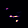
\includegraphics[width=0.12\textwidth]{resultats/LGD/sizes/size_mid2-init-pas=0.1_filtre=s-None.png}
&
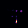
\includegraphics[width=0.12\textwidth]{resultats/LGD/sizes/size_mid1-init-pas=0.1_filtre=s-None.png}
&
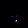
\includegraphics[width=0.12\textwidth]{resultats/LGD/sizes/size_small-init-pas=0.05_filtre=s-None.png}
&
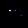
\includegraphics[width=0.12\textwidth]{resultats/LGD/sizes/size_mini-init-pas=0.01_filtre=s-None.png}

\\


&

\includegraphics[width=0.12\textwidth]{resultats/LGD/sizes/size_big-compatarget-s.png}
&

\includegraphics[width=0.12\textwidth]{resultats/LGD/sizes/size_mid2-compatarget-s.png}
&

\includegraphics[height=0.12\textwidth]{resultats/LGD/sizes/size_mid1-compatarget-s.png}
&

\includegraphics[width=0.12\textwidth]{resultats/LGD/sizes/size_small-compatarget-s.png}
&

\includegraphics[width=0.12\textwidth]{resultats/LGD/sizes/size_mini-compatarget-s.png}

\\


&

\includegraphics[width=0.12\textwidth]{resultats/LGD/sizes/size_big-guess-pas=0.1_filtre=s-None.png}
&

\includegraphics[width=0.12\textwidth]{resultats/LGD/sizes/size_mid2-guess-pas=0.1_filtre=s-None.png}
&
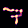
\includegraphics[width=0.12\textwidth]{resultats/LGD/sizes/size_mid1-guess-pas=0.1_filtre=s-None.png}
&
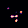
\includegraphics[width=0.12\textwidth]{resultats/LGD/sizes/size_small-guess-pas=0.05_filtre=s-None.png}
&
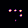
\includegraphics[width=0.12\textwidth]{resultats/LGD/sizes/size_mini-guess-pas=0.01_filtre=s-None.png}

\\ \\



\multicolumn{2}{c}{Loss}  &  \multicolumn{4}{c}{PSNR{\color{white}bbbb}}

\\

\multicolumn{2}{c}{% This file was created with tikzplotlib v0.10.1.
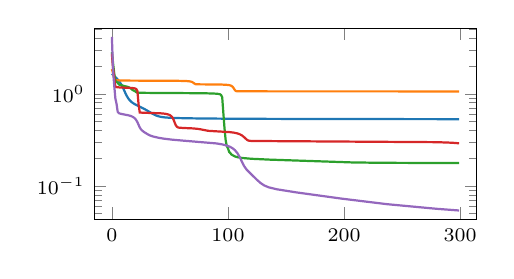
\begin{tikzpicture}

\definecolor{crimson2143940}{RGB}{214,39,40}
\definecolor{darkgray176}{RGB}{176,176,176}
\definecolor{darkorange25512714}{RGB}{255,127,14}
\definecolor{forestgreen4416044}{RGB}{44,160,44}
\definecolor{mediumpurple148103189}{RGB}{148,103,189}
\definecolor{steelblue31119180}{RGB}{31,119,180}

\begin{axis}[compar,
	ymode=log]
\addplot [thick, steelblue31119180]
table {%
0 1.65230560302734
1 1.60967218875885
3 1.51980757713318
5 1.4276807308197
6 1.37903583049774
7 1.32599353790283
8 1.26667380332947
9 1.20057117938995
11 1.05875587463379
12 0.993848085403442
13 0.939155459403992
14 0.895524501800537
15 0.861427426338196
16 0.834641695022583
17 0.813176393508911
18 0.795508742332458
19 0.780535697937012
21 0.755721092224121
24 0.724630355834961
28 0.684367299079895
32 0.640052795410156
35 0.6075519323349
37 0.589563608169556
39 0.575842380523682
41 0.56618332862854
43 0.559664726257324
46 0.553641200065613
50 0.549216270446777
57 0.545149207115173
70 0.541172504425049
93 0.53755521774292
135 0.534475564956665
221 0.531806707382202
299 0.530493259429932
};
\addplot [thick, darkorange25512714]
table {%
0 1.85211646556854
1 1.67770111560822
2 1.46272897720337
3 1.41593718528748
4 1.40484702587128
5 1.39981067180634
7 1.39501214027405
10 1.39188122749329
16 1.38930439949036
32 1.38671922683716
55 1.38247323036194
61 1.37871134281158
64 1.3742892742157
66 1.36830806732178
67 1.36319196224213
68 1.3552680015564
69 1.34236979484558
70 1.32132458686829
71 1.292635679245
72 1.27158439159393
73 1.26629757881165
76 1.26518905162811
89 1.26179456710815
95 1.25753927230835
98 1.25268864631653
100 1.24624443054199
101 1.24075663089752
102 1.23218429088593
103 1.21773552894592
104 1.191610455513
105 1.1454873085022
106 1.09121680259705
107 1.06940352916718
108 1.06570613384247
111 1.06433713436127
144 1.06147050857544
275 1.06137251853943
299 1.06136870384216
};
\addplot [thick, forestgreen4416044]
table {%
0 2.84194612503052
1 2.15506029129028
2 1.66873693466187
3 1.38294208049774
5 1.31623303890228
6 1.26444888114929
7 1.24834167957306
9 1.23046517372131
11 1.20998632907867
13 1.19424068927765
14 1.18405818939209
15 1.1702915430069
16 1.15001618862152
17 1.1210218667984
18 1.09569573402405
19 1.08197319507599
20 1.06478106975555
21 1.0405730009079
22 1.02683997154236
25 1.02437090873718
35 1.02164471149445
77 1.01418256759644
85 1.00862324237823
89 1.00375008583069
91 0.999232292175293
92 0.9952312707901
93 0.988119006156921
94 0.972235679626465
95 0.91933798789978
96 0.616937160491943
97 0.421802282333374
98 0.312908411026001
99 0.270792961120605
100 0.255544066429138
101 0.234020471572876
102 0.227557420730591
103 0.219099283218384
106 0.209146738052368
108 0.20545756816864
112 0.201385498046875
120 0.197391390800476
136 0.193149089813232
207 0.180134654045105
232 0.178421974182129
299 0.177336454391479
};
\addplot [thick, crimson2143940]
table {%
0 2.71224212646484
1 1.89663374423981
2 1.51032817363739
3 1.19073891639709
4 1.18067479133606
6 1.17347884178162
9 1.16805064678192
17 1.15556478500366
19 1.1488208770752
20 1.14171743392944
21 1.12556207180023
22 1.0690438747406
23 0.763562440872192
24 0.626803040504456
26 0.623935461044312
42 0.614003896713257
45 0.609050154685974
47 0.603470325469971
49 0.593772172927856
50 0.585844755172729
51 0.574084281921387
52 0.555935382843018
53 0.527923822402954
54 0.490156412124634
55 0.456605553627014
56 0.438905239105225
57 0.431463479995728
58 0.428577065467834
61 0.426207780838013
70 0.421022057533264
74 0.416285991668701
77 0.410333037376404
83 0.396579504013062
88 0.392909526824951
101 0.38445782661438
105 0.37907612323761
108 0.372137427330017
110 0.364766120910645
112 0.353622436523438
114 0.337481260299683
116 0.319562911987305
117 0.313272714614868
118 0.309869647026062
120 0.30800199508667
132 0.30707573890686
280 0.298706293106079
293 0.294538974761963
299 0.290218830108643
};
\addplot [thick, mediumpurple148103189]
table {%
0 4.13749027252197
1 1.78226494789124
2 1.23609900474548
3 0.890265941619873
4 0.779228687286377
5 0.638609528541565
6 0.617340087890625
7 0.609525799751282
9 0.601629018783569
14 0.585130453109741
16 0.575769901275635
17 0.569563150405884
18 0.561703205108643
19 0.551372528076172
20 0.537355184555054
21 0.517969131469727
22 0.491822361946106
23 0.46056592464447
24 0.431907415390015
25 0.412346363067627
26 0.399762630462646
28 0.382634878158569
31 0.362732648849487
33 0.35280454158783
36 0.34282374382019
40 0.333760499954224
45 0.325755834579468
52 0.317875027656555
63 0.309140682220459
90 0.289501667022705
95 0.28264594078064
99 0.274349570274353
102 0.264988541603088
104 0.256195902824402
106 0.244262218475342
108 0.227995634078979
110 0.206859588623047
113 0.172638773918152
114 0.163624286651611
116 0.150722026824951
119 0.13795006275177
125 0.116512775421143
128 0.107834815979004
131 0.10168719291687
135 0.0967668294906616
142 0.0921484231948853
159 0.0851820707321167
198 0.0729167461395264
237 0.0635035037994385
279 0.0566712617874146
299 0.0542340278625488
};
\end{axis}

\end{tikzpicture}
}
&
\multicolumn{4}{c}{% This file was created with tikzplotlib v0.10.1.
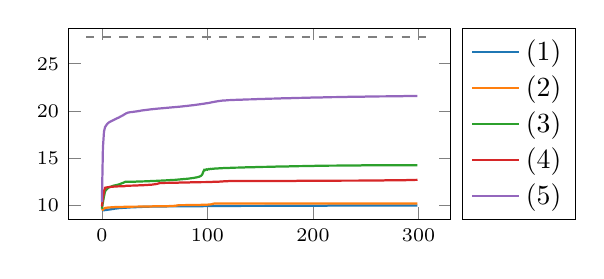
\begin{tikzpicture}

\definecolor{crimson2143940}{RGB}{214,39,40}
\definecolor{darkgray176}{RGB}{176,176,176}
\definecolor{darkorange25512714}{RGB}{255,127,14}
\definecolor{forestgreen4416044}{RGB}{44,160,44}
\definecolor{mediumpurple148103189}{RGB}{148,103,189}
\definecolor{steelblue31119180}{RGB}{31,119,180}

\begin{axis}[compar, legend pos=outer north east]
\addplot [thick, steelblue31119180]
table {%
0 9.43000030517578
1 9.44999980926514
3 9.47000026702881
4 9.48999977111816
5 9.5
6 9.52000045776367
7 9.52999973297119
9 9.56999969482422
10 9.57999992370605
13 9.64000034332275
15 9.65999984741211
16 9.68000030517578
18 9.69999980926514
19 9.69999980926514
22 9.72999954223633
23 9.72999954223633
25 9.75
26 9.75
27 9.76000022888184
28 9.76000022888184
29 9.77000045776367
30 9.77000045776367
31 9.77999973297119
32 9.77999973297119
34 9.80000019073486
35 9.80000019073486
36 9.8100004196167
38 9.8100004196167
39 9.81999969482422
40 9.81999969482422
41 9.82999992370605
44 9.82999992370605
45 9.84000015258789
48 9.84000015258789
49 9.85000038146973
54 9.85000038146973
55 9.85999965667725
61 9.85999965667725
62 9.86999988555908
71 9.86999988555908
72 9.88000011444092
82 9.88000011444092
83 9.89000034332275
96 9.89000034332275
97 9.89999961853027
112 9.89999961853027
113 9.90999984741211
131 9.90999984741211
132 9.92000007629395
154 9.92000007629395
155 9.93000030517578
181 9.93000030517578
182 9.9399995803833
213 9.9399995803833
214 9.94999980926514
251 9.94999980926514
252 9.96000003814697
295 9.96000003814697
296 9.97000026702881
299 9.97000026702881
};
\addlegendentry{$(1)$}
\addplot [thick, darkorange25512714]
table {%
0 9.4399995803833
1 9.52000045776367
2 9.64000034332275
3 9.6899995803833
4 9.72000026702881
5 9.72999954223633
6 9.75
7 9.76000022888184
8 9.76000022888184
10 9.77999973297119
11 9.77999973297119
12 9.78999996185303
14 9.78999996185303
15 9.80000019073486
16 9.80000019073486
17 9.8100004196167
20 9.8100004196167
21 9.81999969482422
24 9.81999969482422
25 9.82999992370605
29 9.82999992370605
30 9.84000015258789
34 9.84000015258789
35 9.85000038146973
40 9.85000038146973
41 9.85999965667725
47 9.85999965667725
48 9.86999988555908
53 9.86999988555908
54 9.88000011444092
59 9.88000011444092
60 9.89000034332275
63 9.89000034332275
64 9.89999961853027
66 9.89999961853027
70 9.9399995803833
72 9.97999954223633
74 10
79 10
80 10.0100002288818
87 10.0100002288818
88 10.0200004577637
93 10.0200004577637
94 10.0299997329712
97 10.0299997329712
98 10.039999961853
99 10.039999961853
103 10.0799999237061
104 10.1000003814697
106 10.1599998474121
107 10.1700000762939
170 10.1700000762939
171 10.1800003051758
299 10.1800003051758
};
\addlegendentry{$(2)$}
\addplot [thick, forestgreen4416044]
table {%
0 9.60999965667725
1 10.289999961853
2 10.9300003051758
3 11.4499998092651
4 11.6199998855591
5 11.710000038147
6 11.8199996948242
7 11.9099998474121
8 11.9399995803833
11 12.0600004196167
12 12.0900001525879
13 12.1099996566772
14 12.1400003433228
15 12.1599998474121
16 12.1899995803833
17 12.2299995422363
18 12.2799997329712
20 12.3599996566772
21 12.4099998474121
22 12.4700002670288
23 12.4799995422363
27 12.4799995422363
28 12.4899997711182
32 12.4899997711182
33 12.5
35 12.5
36 12.5100002288818
38 12.5100002288818
39 12.5200004577637
40 12.5200004577637
41 12.5299997329712
43 12.5299997329712
44 12.539999961853
45 12.539999961853
46 12.5500001907349
47 12.5500001907349
48 12.5600004196167
49 12.5600004196167
50 12.5699996948242
51 12.5699996948242
52 12.5799999237061
53 12.5799999237061
55 12.6000003814697
56 12.6000003814697
57 12.6099996566772
58 12.6099996566772
59 12.6199998855591
60 12.6199998855591
62 12.6400003433228
63 12.6400003433228
65 12.6599998474121
66 12.6599998474121
68 12.6800003051758
69 12.6800003051758
82 12.8100004196167
83 12.8299999237061
84 12.8400001525879
85 12.8599996566772
86 12.8699998855591
90 12.9499998092651
92 13.0100002288818
93 13.0500001907349
94 13.1199998855591
95 13.2299995422363
96 13.5100002288818
97 13.75
98 13.7200002670288
99 13.8000001907349
100 13.7600002288818
101 13.8299999237061
102 13.8100004196167
103 13.8500003814697
104 13.8400001525879
105 13.8699998855591
106 13.8599996566772
107 13.8800001144409
108 13.8800001144409
109 13.8900003433228
110 13.8900003433228
111 13.9099998474121
112 13.9099998474121
113 13.9200000762939
114 13.9200000762939
115 13.9300003051758
117 13.9300003051758
118 13.9399995803833
119 13.9399995803833
120 13.9499998092651
121 13.9499998092651
122 13.960000038147
124 13.960000038147
125 13.9700002670288
126 13.9700002670288
127 13.9799995422363
129 13.9799995422363
130 13.9899997711182
132 13.9899997711182
133 14
135 14
136 14.0100002288818
138 14.0100002288818
139 14.0200004577637
142 14.0200004577637
143 14.0299997329712
145 14.0299997329712
146 14.039999961853
149 14.039999961853
150 14.0500001907349
152 14.0500001907349
153 14.0600004196167
156 14.0600004196167
157 14.0699996948242
160 14.0699996948242
161 14.0799999237061
164 14.0799999237061
165 14.0900001525879
168 14.0900001525879
169 14.1000003814697
172 14.1000003814697
173 14.1099996566772
177 14.1099996566772
178 14.1199998855591
181 14.1199998855591
182 14.1300001144409
186 14.1300001144409
187 14.1400003433228
190 14.1400003433228
191 14.1499996185303
195 14.1499996185303
196 14.1599998474121
201 14.1599998474121
202 14.1700000762939
207 14.1700000762939
208 14.1800003051758
214 14.1800003051758
215 14.1899995803833
222 14.1899995803833
223 14.1999998092651
232 14.1999998092651
233 14.210000038147
245 14.210000038147
246 14.2200002670288
262 14.2200002670288
263 14.2299995422363
281 14.2299995422363
282 14.2399997711182
299 14.2399997711182
};
\addlegendentry{$(3)$}
\addplot [thick, crimson2143940]
table {%
0 9.85000038146973
1 10.7600002288818
2 11.4700002670288
3 11.8400001525879
4 11.8699998855591
5 11.8900003433228
6 11.8999996185303
7 11.9200000762939
12 11.9700002670288
13 11.9700002670288
15 11.9899997711182
16 11.9899997711182
17 12
18 12
19 12.0100002288818
21 12.0100002288818
22 12.0200004577637
23 12.0600004196167
27 12.0600004196167
28 12.0699996948242
29 12.0699996948242
30 12.0799999237061
32 12.0799999237061
33 12.0900001525879
34 12.0900001525879
35 12.1000003814697
36 12.1000003814697
37 12.1099996566772
38 12.1099996566772
39 12.1199998855591
40 12.1199998855591
42 12.1400003433228
43 12.1400003433228
45 12.1599998474121
46 12.1599998474121
48 12.1800003051758
49 12.1999998092651
50 12.210000038147
52 12.25
55 12.3400001525879
56 12.3500003814697
59 12.3500003814697
60 12.3599996566772
63 12.3599996566772
64 12.3699998855591
68 12.3699998855591
69 12.3800001144409
72 12.3800001144409
73 12.3900003433228
76 12.3900003433228
77 12.3999996185303
80 12.3999996185303
81 12.4099998474121
83 12.4099998474121
84 12.4200000762939
88 12.4200000762939
89 12.4300003051758
93 12.4300003051758
94 12.4399995803833
98 12.4399995803833
99 12.4499998092651
101 12.4499998092651
102 12.460000038147
104 12.460000038147
105 12.4700002670288
107 12.4700002670288
108 12.4799995422363
109 12.4799995422363
110 12.4899997711182
111 12.4899997711182
112 12.5
113 12.5
116 12.5299997329712
117 12.5299997329712
118 12.539999961853
119 12.539999961853
120 12.5500001907349
136 12.5500001907349
137 12.5600004196167
160 12.5600004196167
161 12.5699996948242
184 12.5699996948242
185 12.5799999237061
207 12.5799999237061
208 12.5900001525879
226 12.5900001525879
227 12.6000003814697
243 12.6000003814697
244 12.6099996566772
257 12.6099996566772
258 12.6199998855591
267 12.6199998855591
268 12.6300001144409
276 12.6300001144409
277 12.6400003433228
283 12.6400003433228
284 12.6499996185303
288 12.6499996185303
289 12.6599998474121
292 12.6599998474121
293 12.6700000762939
296 12.6700000762939
297 12.6800003051758
298 12.6800003051758
299 12.6899995803833
};
\addlegendentry{$(4)$}
\addplot [thick, mediumpurple148103189]
table {%
0 10.3500003814697
1 16.1200008392334
2 17.7999992370605
3 18.2800006866455
4 18.4400005340576
5 18.6100006103516
6 18.7099990844727
7 18.7999992370605
9 18.9200000762939
10 18.9699993133545
11 19.0300006866455
12 19.0799999237061
13 19.1399993896484
14 19.1900005340576
15 19.25
16 19.2900009155273
17 19.3600006103516
18 19.4099998474121
19 19.4799995422363
20 19.5300006866455
21 19.6100006103516
22 19.6700000762939
23 19.7399997711182
24 19.7800006866455
25 19.8299999237061
26 19.8400001525879
27 19.8700008392334
28 19.8700008392334
29 19.8899993896484
30 19.8999996185303
31 19.9200000762939
32 19.9300003051758
33 19.9500007629395
34 19.9599990844727
35 19.9899997711182
36 20
37 20.0300006866455
38 20.0400009155273
39 20.0599994659424
40 20.0699996948242
41 20.0900001525879
42 20.1000003814697
43 20.1200008392334
44 20.1299991607666
45 20.1499996185303
48 20.1800003051758
49 20.2000007629395
50 20.2000007629395
51 20.2199993133545
76 20.4699993133545
77 20.4899997711182
81 20.5300006866455
82 20.5499992370605
84 20.5699996948242
85 20.5900001525879
87 20.6100006103516
88 20.6299991607666
89 20.6399993896484
90 20.6599998474121
91 20.6700000762939
92 20.6900005340576
93 20.7000007629395
95 20.7399997711182
96 20.75
99 20.8099994659424
100 20.8199996948242
103 20.8799991607666
104 20.9099998474121
111 21.0499992370605
113 21.0699996948242
114 21.0900001525879
116 21.1100006103516
117 21.1100006103516
120 21.1399993896484
121 21.1399993896484
122 21.1499996185303
123 21.1499996185303
124 21.1599998474121
125 21.1599998474121
126 21.1700000762939
127 21.1700000762939
128 21.1800003051758
130 21.1800003051758
131 21.1900005340576
133 21.1900005340576
134 21.2000007629395
135 21.2000007629395
136 21.2099990844727
138 21.2099990844727
139 21.2199993133545
141 21.2199993133545
142 21.2299995422363
143 21.2299995422363
144 21.2399997711182
146 21.2399997711182
147 21.25
149 21.25
150 21.2600002288818
152 21.2600002288818
153 21.2700004577637
154 21.2700004577637
155 21.2800006866455
157 21.2800006866455
158 21.2900009155273
160 21.2900009155273
161 21.2999992370605
163 21.2999992370605
164 21.3099994659424
166 21.3099994659424
167 21.3199996948242
169 21.3199996948242
170 21.3299999237061
172 21.3299999237061
173 21.3400001525879
176 21.3400001525879
177 21.3500003814697
179 21.3500003814697
180 21.3600006103516
182 21.3600006103516
183 21.3700008392334
186 21.3700008392334
187 21.3799991607666
189 21.3799991607666
190 21.3899993896484
193 21.3899993896484
194 21.3999996185303
197 21.3999996185303
198 21.4099998474121
201 21.4099998474121
202 21.4200000762939
205 21.4200000762939
206 21.4300003051758
209 21.4300003051758
210 21.4400005340576
213 21.4400005340576
214 21.4500007629395
217 21.4500007629395
218 21.4599990844727
222 21.4599990844727
223 21.4699993133545
227 21.4699993133545
228 21.4799995422363
232 21.4799995422363
233 21.4899997711182
238 21.4899997711182
239 21.5
243 21.5
244 21.5100002288818
249 21.5100002288818
250 21.5200004577637
255 21.5200004577637
256 21.5300006866455
262 21.5300006866455
263 21.5400009155273
269 21.5400009155273
270 21.5499992370605
277 21.5499992370605
278 21.5599994659424
285 21.5599994659424
286 21.5699996948242
294 21.5699996948242
295 21.5799999237061
299 21.5799999237061
};
\addlegendentry{$(5)$}
\addplot [thick, gray, dashed]
table {%
-14.95 27.8502388000488
313.95 27.8502388000488
};
\end{axis}

\end{tikzpicture}
}
\end{tabular}
	\caption{En première lignes différentes initialisations avec en dessous le résultat de la LGD après 300 itérations -- sans filtre passe-bas}
	\label{fig:LGDinits}
\end{figure}

\begin{figure}[H]\centering
	\begin{tabular}{c c c c c c}
Target  &  $(1)$  &  $(2)$  &  $(3)$  &  $(4)$

\\

\multirow{2}{0.3\textwidth}[0.125\textwidth]{
\includegraphics[width=0.3\textwidth]{resultats/LGD/inits/inits-target-g.png}}
&
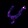
\includegraphics[width=0.15\textwidth]{resultats/LGD/inits/inits_1-init-pas=0.25_filtre=g-0.6.png}
&

\includegraphics[width=0.15\textwidth]{resultats/LGD/inits/inits_2-init-pas=0.25_filtre=g-0.6.png}
&

\includegraphics[width=0.15\textwidth]{resultats/LGD/inits/inits_3-init-pas=0.25_filtre=g-0.6.png}
&

\includegraphics[width=0.15\textwidth]{resultats/LGD/inits/inits_4-init-pas=0.25_filtre=g-0.6.png}

\\


&

\includegraphics[width=0.15\textwidth]{resultats/LGD/inits/inits_1-guess-pas=0.25_filtre=g-0.6.png}
&

\includegraphics[width=0.15\textwidth]{resultats/LGD/inits/inits_2-guess-pas=0.25_filtre=g-0.6.png}
&

\includegraphics[width=0.15\textwidth]{resultats/LGD/inits/inits_3-guess-pas=0.25_filtre=g-0.6.png}
&

\includegraphics[width=0.15\textwidth]{resultats/LGD/inits/inits_4-guess-pas=0.25_filtre=g-0.6.png}

\\ \\



\multicolumn{2}{c}{Loss}  &  \multicolumn{3}{c}{PSNR{\color{white}bbbb}}

\\

\multicolumn{2}{c}{% This file was created with tikzplotlib v0.10.1.
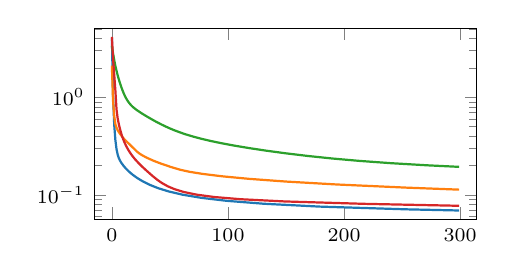
\begin{tikzpicture}

\definecolor{crimson2143940}{RGB}{214,39,40}
\definecolor{darkgray176}{RGB}{176,176,176}
\definecolor{darkorange25512714}{RGB}{255,127,14}
\definecolor{forestgreen4416044}{RGB}{44,160,44}
\definecolor{steelblue31119180}{RGB}{31,119,180}

\begin{axis}[compar,
	ymode=log]
\addplot [thick, steelblue31119180]
table {%
0 4.09705591201782
1 1.0397447347641
2 0.525999307632446
3 0.36544942855835
4 0.294240236282349
5 0.258731842041016
6 0.23837411403656
7 0.2248694896698
8 0.214669942855835
10 0.199013829231262
12 0.18678867816925
15 0.172265887260437
18 0.160792350769043
22 0.148674130439758
27 0.136995673179626
33 0.126390695571899
40 0.117159008979797
49 0.108532667160034
61 0.100532412528992
77 0.0933989286422729
99 0.0870349407196045
131 0.0812307596206665
179 0.0759825706481934
254 0.0712192058563232
299 0.0692975521087646
};
\addplot [thick, darkorange25512714]
table {%
0 2.11676383018494
1 0.9190913438797
2 0.643004417419434
3 0.532035350799561
4 0.487879872322083
5 0.460638880729675
6 0.440029859542847
7 0.422846078872681
9 0.393353462219238
11 0.368957042694092
13 0.349978923797607
22 0.275432348251343
24 0.264232397079468
27 0.25137186050415
31 0.237775444984436
36 0.22367525100708
42 0.210012912750244
51 0.193120121955872
59 0.180989027023315
67 0.172550797462463
78 0.164394378662109
95 0.155235648155212
118 0.146238088607788
150 0.137122750282288
194 0.127958059310913
254 0.118792176246643
299 0.113348960876465
};
\addplot [thick, forestgreen4416044]
table {%
0 3.37779760360718
1 2.81990122795105
2 2.4142701625824
3 2.10492038726807
4 1.86983335018158
5 1.67920529842377
6 1.52351367473602
7 1.3948290348053
8 1.2856605052948
9 1.19226157665253
10 1.11291658878326
11 1.04617238044739
12 0.990375518798828
13 0.94380521774292
14 0.904836654663086
15 0.872018575668335
16 0.844097495079041
17 0.820020079612732
18 0.798925280570984
19 0.780128955841064
21 0.747454047203064
23 0.719166994094849
25 0.693710803985596
28 0.659082055091858
31 0.627551555633545
34 0.598529100418091
38 0.563355803489685
42 0.532020330429077
46 0.504339337348938
50 0.480038523674011
54 0.458757042884827
59 0.435793519020081
64 0.416170716285706
70 0.396113634109497
77 0.376400947570801
85 0.357464551925659
94 0.339470624923706
105 0.320858478546143
118 0.30225658416748
133 0.284092664718628
150 0.266751885414124
169 0.250633358955383
190 0.236100435256958
213 0.223376154899597
240 0.211698055267334
272 0.201091408729553
299 0.194014668464661
};
\addplot [thick, crimson2143940]
table {%
0 4.15872049331665
1 2.48774647712708
2 1.71559143066406
3 1.18148231506348
4 0.74964714050293
5 0.606518745422363
6 0.529028296470642
7 0.472540497779846
8 0.428424477577209
9 0.393683195114136
10 0.365716695785522
11 0.342551231384277
12 0.322939038276672
13 0.306079387664795
14 0.291416645050049
16 0.267123222351074
18 0.247718811035156
20 0.231697797775269
23 0.211907505989075
26 0.195417284965515
30 0.176599979400635
35 0.156593918800354
39 0.143312335014343
43 0.132702112197876
48 0.12282931804657
54 0.114545702934265
62 0.10715639591217
73 0.100697159767151
88 0.0952965021133423
111 0.0903933048248291
149 0.0857839584350586
217 0.0811049938201904
299 0.0774440765380859
};

\end{axis}

\end{tikzpicture}
}
&
\multicolumn{3}{c}{% This file was created with tikzplotlib v0.10.1.
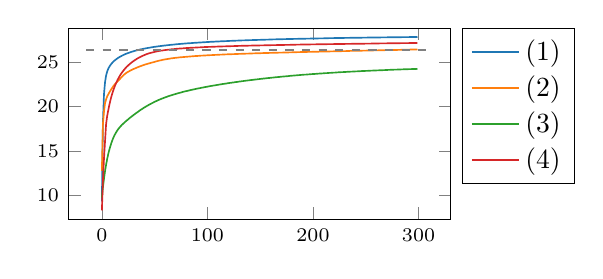
\begin{tikzpicture}

\definecolor{crimson2143940}{RGB}{214,39,40}
\definecolor{darkgray176}{RGB}{176,176,176}
\definecolor{darkorange25512714}{RGB}{255,127,14}
\definecolor{forestgreen4416044}{RGB}{44,160,44}
\definecolor{steelblue31119180}{RGB}{31,119,180}

\begin{axis}[compar, legend pos=outer north east]
\addplot [semithick, steelblue31119180]
table {%
0 9.34000015258789
1 18.2600002288818
2 21.3700008392334
3 22.7199993133545
4 23.4599990844727
5 23.8999996185303
6 24.2099990844727
7 24.4300003051758
8 24.6200008392334
9 24.7700004577637
10 24.9099998474121
11 25.0300006866455
12 25.1399993896484
15 25.4099998474121
16 25.4799995422363
17 25.5599994659424
21 25.7999992370605
24 25.9500007629395
29 26.1499996185303
30 26.1800003051758
31 26.2199993133545
37 26.3999996185303
38 26.4200000762939
39 26.4500007629395
41 26.4899997711182
42 26.5200004577637
50 26.6800003051758
51 26.6900005340576
53 26.7299995422363
54 26.7399997711182
55 26.7600002288818
56 26.7700004577637
57 26.7900009155273
58 26.7999992370605
59 26.8199996948242
61 26.8400001525879
62 26.8600006103516
64 26.8799991607666
65 26.8999996185303
69 26.9400005340576
70 26.9599990844727
82 27.0799999237061
83 27.0799999237061
88 27.1299991607666
89 27.1299991607666
93 27.1700000762939
94 27.1700000762939
96 27.1900005340576
97 27.1900005340576
100 27.2199993133545
101 27.2199993133545
103 27.2399997711182
104 27.2399997711182
105 27.25
106 27.25
108 27.2700004577637
109 27.2700004577637
110 27.2800006866455
111 27.2800006866455
113 27.2999992370605
114 27.2999992370605
115 27.3099994659424
116 27.3099994659424
117 27.3199996948242
118 27.3199996948242
119 27.3299999237061
120 27.3299999237061
121 27.3400001525879
122 27.3400001525879
123 27.3500003814697
124 27.3500003814697
125 27.3600006103516
126 27.3600006103516
127 27.3700008392334
128 27.3700008392334
129 27.3799991607666
130 27.3799991607666
131 27.3899993896484
132 27.3899993896484
133 27.3999996185303
135 27.3999996185303
136 27.4099998474121
137 27.4099998474121
138 27.4200000762939
139 27.4200000762939
140 27.4300003051758
142 27.4300003051758
143 27.4400005340576
144 27.4400005340576
145 27.4500007629395
147 27.4500007629395
148 27.4599990844727
150 27.4599990844727
151 27.4699993133545
153 27.4699993133545
154 27.4799995422363
155 27.4799995422363
156 27.4899997711182
158 27.4899997711182
159 27.5
161 27.5
162 27.5100002288818
164 27.5100002288818
165 27.5200004577637
168 27.5200004577637
169 27.5300006866455
171 27.5300006866455
172 27.5400009155273
174 27.5400009155273
175 27.5499992370605
178 27.5499992370605
179 27.5599994659424
181 27.5599994659424
182 27.5699996948242
185 27.5699996948242
186 27.5799999237061
189 27.5799999237061
190 27.5900001525879
193 27.5900001525879
194 27.6000003814697
197 27.6000003814697
198 27.6100006103516
201 27.6100006103516
202 27.6200008392334
205 27.6200008392334
206 27.6299991607666
210 27.6299991607666
211 27.6399993896484
214 27.6399993896484
215 27.6499996185303
219 27.6499996185303
220 27.6599998474121
224 27.6599998474121
225 27.6700000762939
229 27.6700000762939
230 27.6800003051758
234 27.6800003051758
235 27.6900005340576
240 27.6900005340576
241 27.7000007629395
246 27.7000007629395
247 27.7099990844727
251 27.7099990844727
252 27.7199993133545
257 27.7199993133545
258 27.7299995422363
264 27.7299995422363
265 27.7399997711182
270 27.7399997711182
271 27.75
277 27.75
278 27.7600002288818
284 27.7600002288818
285 27.7700004577637
291 27.7700004577637
292 27.7800006866455
298 27.7800006866455
299 27.7900009155273
};
\addlegendentry{$(1)$}
\addplot [semithick, darkorange25512714]
table {%
0 12.7600002288818
1 18.0300006866455
2 19.4099998474121
3 20.3700008392334
4 20.7800006866455
5 21.1100006103516
7 21.5499992370605
8 21.75
9 21.9400005340576
10 22.1200008392334
11 22.2900009155273
12 22.4400005340576
13 22.5799999237061
16 22.9400005340576
17 23.0699996948242
18 23.1900005340576
19 23.3199996948242
20 23.4400005340576
21 23.5499992370605
22 23.6499996185303
23 23.7399997711182
24 23.8199996948242
25 23.8899993896484
26 23.9500007629395
27 24.0200004577637
28 24.0799999237061
29 24.1299991607666
30 24.1900005340576
36 24.4899997711182
42 24.7299995422363
43 24.7600002288818
44 24.7999992370605
46 24.8600006103516
47 24.8999996185303
50 24.9899997711182
51 25.0300006866455
55 25.1499996185303
56 25.1700000762939
58 25.2299995422363
66 25.3899993896484
67 25.3999996185303
68 25.4200000762939
69 25.4300003051758
70 25.4500007629395
72 25.4699993133545
73 25.4899997711182
89 25.6499996185303
90 25.6499996185303
94 25.6900005340576
95 25.6900005340576
97 25.7099990844727
98 25.7099990844727
100 25.7299995422363
101 25.7299995422363
103 25.75
104 25.75
105 25.7600002288818
106 25.7600002288818
108 25.7800006866455
109 25.7800006866455
110 25.7900009155273
111 25.7900009155273
112 25.7999992370605
113 25.7999992370605
115 25.8199996948242
116 25.8199996948242
117 25.8299999237061
118 25.8299999237061
119 25.8400001525879
120 25.8400001525879
121 25.8500003814697
123 25.8500003814697
124 25.8600006103516
125 25.8600006103516
126 25.8700008392334
127 25.8700008392334
128 25.8799991607666
129 25.8799991607666
130 25.8899993896484
132 25.8899993896484
133 25.8999996185303
134 25.8999996185303
135 25.9099998474121
136 25.9099998474121
137 25.9200000762939
139 25.9200000762939
140 25.9300003051758
142 25.9300003051758
143 25.9400005340576
144 25.9400005340576
145 25.9500007629395
147 25.9500007629395
148 25.9599990844727
150 25.9599990844727
151 25.9699993133545
152 25.9699993133545
153 25.9799995422363
155 25.9799995422363
156 25.9899997711182
158 25.9899997711182
159 26
161 26
162 26.0100002288818
164 26.0100002288818
165 26.0200004577637
167 26.0200004577637
168 26.0300006866455
171 26.0300006866455
172 26.0400009155273
174 26.0400009155273
175 26.0499992370605
177 26.0499992370605
178 26.0599994659424
180 26.0599994659424
181 26.0699996948242
184 26.0699996948242
185 26.0799999237061
187 26.0799999237061
188 26.0900001525879
191 26.0900001525879
192 26.1000003814697
194 26.1000003814697
195 26.1100006103516
198 26.1100006103516
199 26.1200008392334
201 26.1200008392334
202 26.1299991607666
205 26.1299991607666
206 26.1399993896484
208 26.1399993896484
209 26.1499996185303
212 26.1499996185303
213 26.1599998474121
216 26.1599998474121
217 26.1700000762939
219 26.1700000762939
220 26.1800003051758
223 26.1800003051758
224 26.1900005340576
227 26.1900005340576
228 26.2000007629395
231 26.2000007629395
232 26.2099990844727
234 26.2099990844727
235 26.2199993133545
238 26.2199993133545
239 26.2299995422363
242 26.2299995422363
243 26.2399997711182
246 26.2399997711182
247 26.25
250 26.25
251 26.2600002288818
253 26.2600002288818
254 26.2700004577637
257 26.2700004577637
258 26.2800006866455
261 26.2800006866455
262 26.2900009155273
265 26.2900009155273
266 26.2999992370605
268 26.2999992370605
269 26.3099994659424
272 26.3099994659424
273 26.3199996948242
276 26.3199996948242
277 26.3299999237061
280 26.3299999237061
281 26.3400001525879
283 26.3400001525879
284 26.3500003814697
287 26.3500003814697
288 26.3600006103516
291 26.3600006103516
292 26.3700008392334
295 26.3700008392334
296 26.3799991607666
298 26.3799991607666
299 26.3899993896484
};
\addlegendentry{$(2)$}
\addplot [semithick, forestgreen4416044]
table {%
0 9.77999973297119
1 10.9300003051758
2 11.8999996185303
3 12.7399997711182
4 13.460000038147
5 14.0900001525879
6 14.6400003433228
7 15.1099996566772
8 15.5299997329712
9 15.8999996185303
10 16.2299995422363
11 16.5200004577637
12 16.7700004577637
13 16.9899997711182
14 17.1900005340576
15 17.3700008392334
16 17.5300006866455
17 17.6700000762939
19 17.9300003051758
22 18.2600002288818
27 18.7600002288818
32 19.2099990844727
33 19.2900009155273
34 19.3799991607666
35 19.4599990844727
36 19.5499992370605
37 19.6299991607666
38 19.7000007629395
40 19.8600006103516
45 20.2099990844727
51 20.5699996948242
52 20.6200008392334
53 20.6800003051758
57 20.8799991607666
58 20.9200000762939
59 20.9699993133545
61 21.0499992370605
62 21.1000003814697
65 21.2199993133545
66 21.25
68 21.3299999237061
69 21.3600006103516
70 21.3999996185303
71 21.4300003051758
72 21.4699993133545
75 21.5599994659424
76 21.6000003814697
79 21.6900005340576
80 21.7099990844727
84 21.8299999237061
85 21.8500003814697
87 21.9099998474121
88 21.9300003051758
89 21.9599990844727
90 21.9799995422363
91 22.0100002288818
93 22.0499992370605
94 22.0799999237061
96 22.1200008392334
97 22.1499996185303
100 22.2099990844727
101 22.2399997711182
115 22.5200004577637
116 22.5300006866455
121 22.6299991607666
122 22.6399993896484
124 22.6800003051758
125 22.6900005340576
127 22.7299995422363
128 22.7399997711182
130 22.7800006866455
131 22.7900009155273
133 22.8299999237061
134 22.8400001525879
135 22.8600006103516
136 22.8700008392334
137 22.8899993896484
138 22.8999996185303
139 22.9200000762939
140 22.9300003051758
141 22.9500007629395
142 22.9599990844727
143 22.9799995422363
144 22.9899997711182
145 23.0100002288818
147 23.0300006866455
148 23.0499992370605
149 23.0599994659424
150 23.0799999237061
152 23.1000003814697
153 23.1200008392334
155 23.1399993896484
156 23.1599998474121
159 23.1900005340576
160 23.2099990844727
163 23.2399997711182
164 23.2600002288818
168 23.2999992370605
169 23.3199996948242
177 23.3999996185303
178 23.4200000762939
192 23.5599994659424
193 23.5599994659424
201 23.6399993896484
202 23.6399993896484
207 23.6900005340576
208 23.6900005340576
212 23.7299995422363
213 23.7299995422363
216 23.7600002288818
217 23.7600002288818
220 23.7900009155273
221 23.7900009155273
224 23.8199996948242
225 23.8199996948242
227 23.8400001525879
228 23.8400001525879
230 23.8600006103516
231 23.8600006103516
233 23.8799991607666
234 23.8799991607666
236 23.8999996185303
237 23.8999996185303
238 23.9099998474121
239 23.9099998474121
241 23.9300003051758
242 23.9300003051758
243 23.9400005340576
244 23.9400005340576
246 23.9599990844727
247 23.9599990844727
248 23.9699993133545
249 23.9699993133545
250 23.9799995422363
251 23.9799995422363
253 24
254 24
255 24.0100002288818
256 24.0100002288818
257 24.0200004577637
258 24.0200004577637
259 24.0300006866455
260 24.0300006866455
261 24.0400009155273
262 24.0400009155273
263 24.0499992370605
264 24.0499992370605
265 24.0599994659424
266 24.0599994659424
267 24.0699996948242
268 24.0699996948242
269 24.0799999237061
270 24.0799999237061
271 24.0900001525879
272 24.0900001525879
273 24.1000003814697
274 24.1000003814697
275 24.1100006103516
276 24.1100006103516
277 24.1200008392334
279 24.1200008392334
280 24.1299991607666
281 24.1299991607666
282 24.1399993896484
283 24.1399993896484
284 24.1499996185303
285 24.1499996185303
286 24.1599998474121
288 24.1599998474121
289 24.1700000762939
290 24.1700000762939
291 24.1800003051758
293 24.1800003051758
294 24.1900005340576
295 24.1900005340576
296 24.2000007629395
298 24.2000007629395
299 24.2099990844727
};
\addlegendentry{$(3)$}
\addplot [semithick, crimson2143940]
table {%
0 8.32999992370605
1 11.6999998092651
2 14.1499996185303
3 16.1100006103516
4 18.0300006866455
5 18.9099998474121
6 19.5400009155273
7 20.1200008392334
8 20.6399993896484
9 21.1000003814697
10 21.5
11 21.8600006103516
12 22.1900005340576
13 22.4799995422363
14 22.75
15 23
16 23.2199993133545
17 23.4300003051758
18 23.6200008392334
19 23.7900009155273
20 23.9500007629395
21 24.1000003814697
22 24.2399997711182
23 24.3700008392334
24 24.4899997711182
26 24.7099990844727
28 24.9099998474121
29 25
30 25.0799999237061
31 25.1700000762939
32 25.2399997711182
33 25.3199996948242
35 25.4599990844727
38 25.6399993896484
42 25.8400001525879
45 25.9599990844727
51 26.1399993896484
53 26.1800003051758
54 26.2099990844727
56 26.25
57 26.2600002288818
60 26.3199996948242
61 26.3299999237061
62 26.3500003814697
64 26.3700008392334
65 26.3899993896484
69 26.4300003051758
70 26.4500007629395
74 26.4899997711182
75 26.4899997711182
80 26.5400009155273
81 26.5400009155273
84 26.5699996948242
85 26.5699996948242
87 26.5900001525879
88 26.5900001525879
90 26.6100006103516
91 26.6100006103516
92 26.6200008392334
93 26.6200008392334
94 26.6299991607666
95 26.6299991607666
97 26.6499996185303
98 26.6499996185303
99 26.6599998474121
100 26.6599998474121
101 26.6700000762939
103 26.6700000762939
104 26.6800003051758
105 26.6800003051758
106 26.6900005340576
107 26.6900005340576
108 26.7000007629395
109 26.7000007629395
110 26.7099990844727
112 26.7099990844727
113 26.7199993133545
114 26.7199993133545
115 26.7299995422363
117 26.7299995422363
118 26.7399997711182
120 26.7399997711182
121 26.75
122 26.75
123 26.7600002288818
125 26.7600002288818
126 26.7700004577637
128 26.7700004577637
129 26.7800006866455
131 26.7800006866455
132 26.7900009155273
135 26.7900009155273
136 26.7999992370605
138 26.7999992370605
139 26.8099994659424
141 26.8099994659424
142 26.8199996948242
145 26.8199996948242
146 26.8299999237061
149 26.8299999237061
150 26.8400001525879
153 26.8400001525879
154 26.8500003814697
156 26.8500003814697
157 26.8600006103516
160 26.8600006103516
161 26.8700008392334
165 26.8700008392334
166 26.8799991607666
169 26.8799991607666
170 26.8899993896484
173 26.8899993896484
174 26.8999996185303
178 26.8999996185303
179 26.9099998474121
183 26.9099998474121
184 26.9200000762939
187 26.9200000762939
188 26.9300003051758
192 26.9300003051758
193 26.9400005340576
197 26.9400005340576
198 26.9500007629395
202 26.9500007629395
203 26.9599990844727
208 26.9599990844727
209 26.9699993133545
213 26.9699993133545
214 26.9799995422363
219 26.9799995422363
220 26.9899997711182
225 26.9899997711182
226 27
230 27
231 27.0100002288818
236 27.0100002288818
237 27.0200004577637
243 27.0200004577637
244 27.0300006866455
249 27.0300006866455
250 27.0400009155273
255 27.0400009155273
256 27.0499992370605
262 27.0499992370605
263 27.0599994659424
269 27.0599994659424
270 27.0699996948242
275 27.0699996948242
276 27.0799999237061
282 27.0799999237061
283 27.0900001525879
290 27.0900001525879
291 27.1000003814697
297 27.1000003814697
298 27.1100006103516
299 27.1100006103516
};
\addlegendentry{$(4)$}
\addplot [semithick, gray,  dashed]
table {%
-14.95 26.3238544464111
313.95 26.3238544464111
};
\end{axis}

\end{tikzpicture}
}
\end{tabular}
	\caption{En premières lignes différentes initialisations avec en dessous le résultat de la LGD après 300 itérations --  avec passe-bas gaussien ($\sigma=0.5$)}
	\label{fig:LGDinitg}
\end{figure}

Il va de soi que le calcul de PSNR est à but purement indicatif et n'intervient pas dans la LGD elle-même. Les ligne en pointillées représentent PSNR$\big(\bf{x_0},f(\bf{x_0})\big)$, le PSNR entre la cible $\bf{x_0}$ est sa version auto-encodée.
Dans la première figure \textit{\ref{fig:LGDinits}} il n'y pas de filtre passe-bas (\ei $A=S$) et dans la seconde \textit{\ref{fig:LGDinitg}}, $C_{\bf{h}}$ est un filtre gaussien de paramètre $\sigma=0.6$ (voir section \ref{sec:forma2pb} pour un rappel sur $\sigma$).
\\
Les différentes initialisations sont les suivantes :
\begin{enumerate}[label=(\arabic*)]
	\item $\bf{u_0}=f_E(^tA\bf{y_0})$, la backprojection encodée de $\bf{y_0}$
	\item $\bf{u_0}=f_E(\bf{x_0})+e$, l'image cible encodée puis bruité (bruit uniforme sur $]-0.5,0.5[$)
	\item idem, avec un bruit gaussien d'écart-type $0.5$
	\item $\bf{u_0}=\bf{u}_{\text{rand}}$,  vecteur aléatoire de l'espace latent
\end{enumerate}

\noindent La première initialisation est la plus naturelle puisqu'elle utilise $^tA$, ce qui se rapproche le plus d'un inverse pour $A$ (voire \textit{fig. \ref{fig:Sapplication}, \ref{fig:passebas-g} \& \ref{fig:passebas-p}} en annexe \ref{anx:gradF} pour les visuels) et de même pour $f_E$ par rapport à $f_D$.
\\
Les initialisations $(2)$ et $(3)$ sont au voisinage de la cible pour voir à quel point il est possible de s'éloigner de $\bf{x_0}$ tout en conservant la convergence de l'algorithme.
\\

Le premier constat est que la méthode fonctionne et ceux même en partant d'un vecteur aléatoire.  Aussi, même s'ils sont meilleurs avec un passe-bas, les résultats restent satisfaisants sans filtre. La structure très simple du jeu de données aide probablement sur ce point et il serait intéressant de voir si les différences avec/sans filtre sont plus marquées sur un jeu de données plus complexe comme Fashion-MNIST.
\\
De plus, les courbes de loss de la figure \textit{\ref{fig:LGDinitg}} n'ont pas toutes finies de descendre (\ei ne sont pas plates à $x=300$) et c'est une remarque que l'on pourra faire sur beaucoup des graphes à suivre dès qu'il y a un filtre passe-bas. Il aurait fallu pousser le nombre d'itérations mais l'algorithme étant lent, on s'est arrêté en bout de 300 par manque de moyen. Cela dit, dans la plupart des cas ce n'est pas un problème au vu de la qualité des reconstructions.
\\
Pour les cas sans passe-bas, les courbes ont tendance à passer par des plateaux, suggérant que la loss puisse encore diminuer en ajoutant de l’inertie à la descente.
\\

Autre chose remarquable, le résultat $(4)$ est meilleur que le $(3)$ alors que l'initialisation du premier est plus éloigné de la cible que le second. Cela est dû à la façon dont est tiré $\bf{u}_{\text{rand}}$. Pour rester cohérent avec la structure des images, et le réseau $f$ (composé de sigmoïde), les coefficients de $\bf{u}_{\text{rand}}$ sont tirés suivant une loi uniforme sur $[0,1]$ et l'auto encodeur gère très mal les vecteurs à valeurs trop loin de l'intervalle $[0,1]$.
\\
Les figures \textit{\ref{fig:LGDgauss-s}} et \textit{\ref{fig:LGDgauss-g}} page suivante, mettent cela en évidence. Chaque ligne correspond à une descente avec en première ligne l'initialisation (décodée), en deuxième la reconstruction dont la cible est en troisième ligne. Les coefficients des initialisations sont tirés suivant une loi normale d'écart-type 2. En comparaison, les initialisations de la figure \textit{\ref{fig:LGDunif-g}} ci-dessous ont été tirées suivant une loi uniforme sur $[0,1]$.

\begin{figure}[H]\centering
	\begin{tabular}{c c c c c c c c c}
$(1)$  &  $(2)$  &  $(3)$  &  $(4)$  &  $(5)$  &  $(6)$  &  $(7)$  &  $(8)$
	
\\

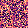
\includegraphics[width=0.1\textwidth]{resultats/PGD/multitarget/rand_unif_1-init-pas=4.25_filtre=g-0.6}
&
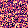
\includegraphics[width=0.1\textwidth]{resultats/PGD/multitarget/rand_unif_2-init-pas=4.25_filtre=g-0.6}
&
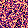
\includegraphics[width=0.1\textwidth]{resultats/PGD/multitarget/rand_unif_3-init-pas=4.25_filtre=g-0.6}
&
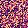
\includegraphics[width=0.1\textwidth]{resultats/PGD/multitarget/rand_unif_4-init-pas=4.25_filtre=g-0.6}
&
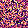
\includegraphics[width=0.1\textwidth]{resultats/PGD/multitarget/rand_unif_5-init-pas=4.25_filtre=g-0.6}
&
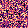
\includegraphics[width=0.1\textwidth]{resultats/PGD/multitarget/rand_unif_6-init-pas=4.25_filtre=g-0.6}
&
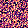
\includegraphics[width=0.1\textwidth]{resultats/PGD/multitarget/rand_unif_7-init-pas=4.25_filtre=g-0.6}
&
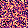
\includegraphics[width=0.1\textwidth]{resultats/PGD/multitarget/rand_unif_8-init-pas=4.25_filtre=g-0.6}

\\


\includegraphics[width=0.1\textwidth]{resultats/PGD/multitarget/rand_unif_1-guess-pas=4.25_filtre=g-0.6}
&

\includegraphics[width=0.1\textwidth]{resultats/PGD/multitarget/rand_unif_2-guess-pas=4.25_filtre=g-0.6}
&
\includegraphics[width=0.1\textwidth]{resultats/PGD/multitarget/rand_unif_3-guess-pas=4.25_filtre=g-0.6}
&
\includegraphics[width=0.1\textwidth]{resultats/PGD/multitarget/rand_unif_4-guess-pas=4.25_filtre=g-0.6}
&
\includegraphics[width=0.1\textwidth]{resultats/PGD/multitarget/rand_unif_5-guess-pas=4.25_filtre=g-0.6}
&
\includegraphics[width=0.1\textwidth]{resultats/PGD/multitarget/rand_unif_6-guess-pas=4.25_filtre=g-0.6}
&
\includegraphics[width=0.1\textwidth]{resultats/PGD/multitarget/rand_unif_7-guess-pas=4.25_filtre=g-0.6}
&
\includegraphics[width=0.1\textwidth]{resultats/PGD/multitarget/rand_unif_8-guess-pas=4.25_filtre=g-0.6}

\\

\includegraphics[width=0.1\textwidth]{resultats/PGD/multitarget/rand_unif_1-target-pas=4.25_filtre=g-0.6}
&
\includegraphics[width=0.1\textwidth]{resultats/PGD/multitarget/rand_unif_2-target-pas=4.25_filtre=g-0.6}
&
\includegraphics[width=0.1\textwidth]{resultats/PGD/multitarget/rand_unif_3-target-pas=4.25_filtre=g-0.6}
&
\includegraphics[width=0.1\textwidth]{resultats/PGD/multitarget/rand_unif_4-target-pas=4.25_filtre=g-0.6}
&
\includegraphics[width=0.1\textwidth]{resultats/PGD/multitarget/rand_unif_5-target-pas=4.25_filtre=g-0.6}
&
\includegraphics[width=0.1\textwidth]{resultats/PGD/multitarget/rand_unif_6-target-pas=4.25_filtre=g-0.6}
&
\includegraphics[width=0.1\textwidth]{resultats/PGD/multitarget/rand_unif_7-target-pas=4.25_filtre=g-0.6}
&
\includegraphics[width=0.1\textwidth]{resultats/PGD/multitarget/rand_unif_8-target-pas=4.25_filtre=g-0.6}

\\ \\



\multicolumn{4}{c}{Loss}  &  \multicolumn{5}{c}{PSNR{\color{white}bbbb}}

\\

\multicolumn{4}{c}{% This file was created with tikzplotlib v0.10.1.
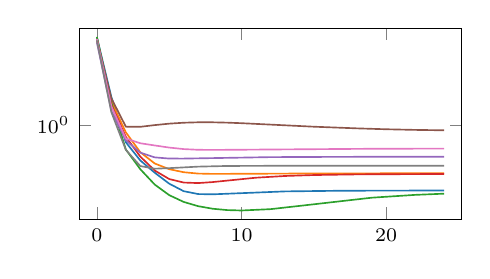
\begin{tikzpicture}

\definecolor{crimson2143940}{RGB}{214,39,40}
\definecolor{darkgray176}{RGB}{176,176,176}
\definecolor{darkorange25512714}{RGB}{255,127,14}
\definecolor{forestgreen4416044}{RGB}{44,160,44}
\definecolor{gray127}{RGB}{127,127,127}
\definecolor{mediumpurple148103189}{RGB}{148,103,189}
\definecolor{orchid227119194}{RGB}{227,119,194}
\definecolor{sienna1408675}{RGB}{140,86,75}
\definecolor{steelblue31119180}{RGB}{31,119,180}

\begin{axis}[compar,
	ymode=log]
\addplot [semithick, steelblue31119180]
table {%
0 6.6873927116394
1 1.8382842540741
2 0.689482450485229
3 0.464741587638855
4 0.356457471847534
5 0.281157732009888
6 0.238898277282715
7 0.224451065063477
8 0.223234534263611
13 0.237807869911194
17 0.24135959148407
24 0.242448091506958
};
\addplot [semithick, darkorange25512714]
table {%
0 6.45488452911377
1 1.66846358776093
2 0.854853868484497
3 0.555467844009399
4 0.435191035270691
5 0.384783029556274
6 0.360276699066162
7 0.349887132644653
8 0.34734034538269
15 0.350641131401062
24 0.352791547775269
};
\addplot [semithick, forestgreen4416044]
table {%
0 6.74908208847046
1 1.62413740158081
2 0.589171409606934
3 0.384576678276062
4 0.275595784187317
5 0.219318866729736
6 0.189371347427368
7 0.172693848609924
8 0.163402318954468
9 0.158696413040161
10 0.157270789146423
12 0.16193413734436
14 0.173686265945435
19 0.20749568939209
22 0.220578670501709
24 0.226373672485352
};
\addplot [semithick, crimson2143940]
table {%
0 6.46834373474121
1 1.53721284866333
2 0.775485038757324
3 0.505563735961914
4 0.373771667480469
5 0.310761332511902
6 0.288039445877075
7 0.284793138504028
8 0.291006684303284
11 0.319954872131348
13 0.332108616828918
15 0.338951945304871
18 0.343920707702637
24 0.346894860267639
};
\addplot [semithick, mediumpurple148103189]
table {%
0 5.98575782775879
1 1.35711002349854
2 0.718473076820374
3 0.550701856613159
4 0.496859669685364
5 0.484203457832336
6 0.483969569206238
12 0.499547839164734
17 0.50269889831543
24 0.503201842308044
};
\addplot [semithick, sienna1408675]
table {%
0 6.31420469284058
1 1.78663504123688
2 0.966158866882324
3 0.963186025619507
4 0.999682307243347
5 1.03141510486603
6 1.05243015289307
7 1.06204438209534
8 1.06177294254303
9 1.0541398525238
10 1.04162240028381
15 0.965239763259888
18 0.930991888046265
20 0.913303852081299
22 0.900914192199707
24 0.892729878425598
};
\addplot [semithick, orchid227119194]
table {%
0 6.43297863006592
1 1.49969029426575
2 0.747458696365356
3 0.67473316192627
4 0.643126964569092
5 0.61441445350647
6 0.594533920288086
7 0.585631370544434
8 0.583965182304382
19 0.598673105239868
24 0.60092830657959
};
\addplot [semithick, gray127]
table {%
0 6.25966119766235
1 1.32219290733337
2 0.585516333580017
3 0.411669135093689
4 0.388913631439209
5 0.39346170425415
7 0.406629323959351
9 0.412495374679565
13 0.414455652236938
24 0.414572954177856
};
\end{axis}

\end{tikzpicture}
}
&
\multicolumn{5}{c}{% This file was created with tikzplotlib v0.10.1.
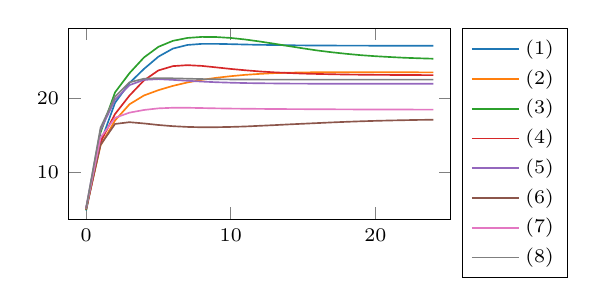
\begin{tikzpicture}

\definecolor{crimson2143940}{RGB}{214,39,40}
\definecolor{darkgray176}{RGB}{176,176,176}
\definecolor{darkorange25512714}{RGB}{255,127,14}
\definecolor{forestgreen4416044}{RGB}{44,160,44}
\definecolor{gray127}{RGB}{127,127,127}
\definecolor{mediumpurple148103189}{RGB}{148,103,189}
\definecolor{orchid227119194}{RGB}{227,119,194}
\definecolor{sienna1408675}{RGB}{140,86,75}
\definecolor{steelblue31119180}{RGB}{31,119,180}

\begin{axis}[compar, legend pos=outer north east]
\addplot [semithick, steelblue31119180]
table {%
0 4.80000019073486
1 13.9700002670288
2 19.3600006103516
3 22.0400009155273
4 23.9400005340576
5 25.6000003814697
6 26.6900005340576
7 27.1800003051758
8 27.3299999237061
9 27.3299999237061
10 27.2900009155273
11 27.2399997711182
12 27.2000007629395
14 27.1399993896484
15 27.1200008392334
18 27.0900001525879
19 27.0900001525879
20 27.0799999237061
24 27.0799999237061
 };
\addlegendentry{\scriptsize{$(1)$}}
\addplot [semithick, darkorange25512714]
table {%
0 4.94999980926514
1 13.6099996566772
2 16.9699993133545
3 19.1599998474121
4 20.3500003814697
5 21.0699996948242
6 21.6499996185303
7 22.1100006103516
8 22.4599990844727
9 22.7399997711182
10 22.9599990844727
11 23.1399993896484
12 23.2700004577637
13 23.3700008392334
14 23.4300003051758
15 23.4699993133545
16 23.4899997711182
17 23.5
20 23.5
21 23.4899997711182
22 23.4899997711182
23 23.4799995422363
24 23.4799995422363
 };
\addlegendentry{\scriptsize{$(2)$}}
\addplot [semithick, forestgreen4416044]
table {%
0 4.84000015258789
1 15.3299999237061
2 20.7700004577637
3 23.3700008392334
4 25.4899997711182
5 26.9300003051758
6 27.7399997711182
7 28.1299991607666
8 28.2700004577637
9 28.25
10 28.1299991607666
11 27.9200000762939
12 27.6499996185303
13 27.3500003814697
14 27.0300006866455
15 26.7199993133545
16 26.4300003051758
17 26.1900005340576
18 25.9799995422363
19 25.7999992370605
20 25.6599998474121
21 25.5499992370605
22 25.4500007629395
23 25.3799991607666
24 25.3199996948242
 };
\addlegendentry{\scriptsize{$(3)$}}
\addplot [semithick, crimson2143940]
table {%
0 4.94000005722046
1 14.0900001525879
2 17.8400001525879
3 20.3400001525879
4 22.3899993896484
5 23.7399997711182
6 24.3199996948242
7 24.4500007629395
8 24.3500003814697
9 24.1499996185303
10 23.9400005340576
11 23.7600002288818
12 23.6000003814697
13 23.4799995422363
14 23.3899993896484
15 23.3099994659424
16 23.2600002288818
18 23.1800003051758
20 23.1399993896484
24 23.1000003814697
 };
\addlegendentry{\scriptsize{$(4)$}}
\addplot [semithick, mediumpurple148103189]
table {%
0 5.17999982833862
1 15.6899995803833
2 19.7700004577637
3 21.75
4 22.4599990844727
5 22.5599994659424
6 22.4599990844727
7 22.3400001525879
8 22.2299995422363
9 22.1399993896484
10 22.0799999237061
11 22.0300006866455
12 22
14 21.9599990844727
16 21.9400005340576
17 21.9400005340576
18 21.9300003051758
24 21.9300003051758
 };
\addlegendentry{\scriptsize{$(5)$}}
\addplot [semithick, sienna1408675]
table {%
0 5.1100001335144
1 13.6700000762939
2 16.5
3 16.7399997711182
4 16.5699996948242
5 16.3600006103516
6 16.2000007629395
7 16.1000003814697
8 16.0499992370605
9 16.0599994659424
10 16.1000003814697
11 16.1599998474121
13 16.3400001525879
14 16.4400005340576
17 16.7099990844727
18 16.7900009155273
19 16.8600006103516
20 16.9200000762939
21 16.9699993133545
23 17.0499992370605
24 17.0699996948242
 };
\addlegendentry{\scriptsize{$(6)$}}
\addplot [semithick, orchid227119194]
table {%
0 5.05000019073486
1 14.6599998474121
2 17.3299999237061
3 18.0300006866455
4 18.3899993896484
5 18.6100006103516
6 18.6900005340576
7 18.6900005340576
9 18.6100006103516
10 18.5799999237061
13 18.5200004577637
19 18.4599990844727
20 18.4599990844727
21 18.4500007629395
22 18.4500007629395
23 18.4400005340576
24 18.4400005340576
 };
\addlegendentry{\scriptsize{$(7)$}}
\addplot [semithick, gray127]
table {%
0 5.07000017166138
1 15.9899997711182
2 20.1800003051758
3 22.1299991607666
4 22.6200008392334
5 22.7000007629395
6 22.6700000762939
8 22.5699996948242
9 22.5400009155273
10 22.5200004577637
13 22.4899997711182
24 22.4899997711182
 };
\addlegendentry{\scriptsize{$(8)$}}
\end{axis}

\end{tikzpicture}
}
\end{tabular}
	\caption{Résultats de LGD toutes initialiser par un vecteur tiré suivant une lui uniforme sur $[0,1]$ ---  avec passe-bas gaussien ($\sigma=0.6$)}
	\label{fig:LGDunif-g}
\end{figure}
\begin{figure}[H]\centering
	\begin{tabular}{c c c c c c c c c}
	$(1)$  &  $(2)$  &  $(3)$  &  $(4)$  &  $(5)$  &  $(6)$  &  $(7)$  &  $(8)$
	
	\\
	
	\includegraphics[width=0.1\textwidth]{resultats/LGD/multitarget/gauss_1-init-pas=0.05_filtre=s-None}
	&
	\includegraphics[width=0.1\textwidth]{resultats/LGD/multitarget/gauss_2-init-pas=0.05_filtre=s-None}
	&
	\includegraphics[width=0.1\textwidth]{resultats/LGD/multitarget/gauss_3-init-pas=0.05_filtre=s-None}
	&
	\includegraphics[width=0.1\textwidth]{resultats/LGD/multitarget/gauss_4-init-pas=0.05_filtre=s-None}
	&
	\includegraphics[width=0.1\textwidth]{resultats/LGD/multitarget/gauss_5-init-pas=0.05_filtre=s-None}
	&
	\includegraphics[width=0.1\textwidth]{resultats/LGD/multitarget/gauss_6-init-pas=0.05_filtre=s-None}
	&
	\includegraphics[width=0.1\textwidth]{resultats/LGD/multitarget/gauss_7-init-pas=0.05_filtre=s-None}
	&
	\includegraphics[width=0.1\textwidth]{resultats/LGD/multitarget/gauss_8-init-pas=0.05_filtre=s-None}
	
	\\
	
	\includegraphics[width=0.1\textwidth]{resultats/LGD/multitarget/gauss_1-guess-pas=0.05_filtre=s-None}
	&
	\includegraphics[width=0.1\textwidth]{resultats/LGD/multitarget/gauss_2-guess-pas=0.05_filtre=s-None}
	&
	\includegraphics[width=0.1\textwidth]{resultats/LGD/multitarget/gauss_3-guess-pas=0.05_filtre=s-None}
	&
	\includegraphics[width=0.1\textwidth]{resultats/LGD/multitarget/gauss_4-guess-pas=0.05_filtre=s-None}
	&
	\includegraphics[width=0.1\textwidth]{resultats/LGD/multitarget/gauss_5-guess-pas=0.05_filtre=s-None}
	&
	\includegraphics[width=0.1\textwidth]{resultats/LGD/multitarget/gauss_6-guess-pas=0.05_filtre=s-None}
	&
	\includegraphics[width=0.1\textwidth]{resultats/LGD/multitarget/gauss_7-guess-pas=0.05_filtre=s-None}
	&
	\includegraphics[width=0.1\textwidth]{resultats/LGD/multitarget/gauss_8-guess-pas=0.05_filtre=s-None}
	
	\\
	
	\includegraphics[width=0.1\textwidth]{resultats/LGD/multitarget/gauss_1-target-pas=0.05_filtre=s-None}
	&
	\includegraphics[width=0.1\textwidth]{resultats/LGD/multitarget/gauss_2-target-pas=0.05_filtre=s-None}
	&
	\includegraphics[width=0.1\textwidth]{resultats/LGD/multitarget/gauss_3-target-pas=0.05_filtre=s-None}
	&
	\includegraphics[width=0.1\textwidth]{resultats/LGD/multitarget/gauss_4-target-pas=0.05_filtre=s-None}
	&
	\includegraphics[width=0.1\textwidth]{resultats/LGD/multitarget/gauss_5-target-pas=0.05_filtre=s-None}
	&
	\includegraphics[width=0.1\textwidth]{resultats/LGD/multitarget/gauss_6-target-pas=0.05_filtre=s-None}
	&
	\includegraphics[width=0.1\textwidth]{resultats/LGD/multitarget/gauss_7-target-pas=0.05_filtre=s-None}
	&
	\includegraphics[width=0.1\textwidth]{resultats/LGD/multitarget/gauss_8-target-pas=0.05_filtre=s-None}
	
	\\ \\
	
	
	
	\multicolumn{4}{c}{Loss}  &  \multicolumn{5}{c}{PSNR{\color{white}bbbb}}
	
	\\
	
	\multicolumn{4}{c}{% This file was created with tikzplotlib v0.10.1.
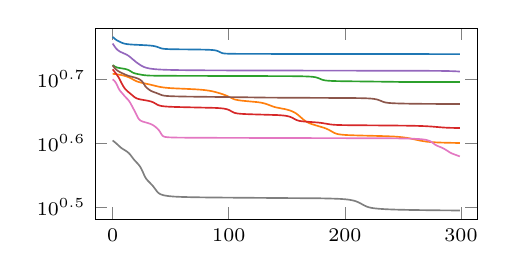
\begin{tikzpicture}

\definecolor{crimson2143940}{RGB}{214,39,40}
\definecolor{darkgray176}{RGB}{176,176,176}
\definecolor{darkorange25512714}{RGB}{255,127,14}
\definecolor{forestgreen4416044}{RGB}{44,160,44}
\definecolor{gray127}{RGB}{127,127,127}
\definecolor{mediumpurple148103189}{RGB}{148,103,189}
\definecolor{orchid227119194}{RGB}{227,119,194}
\definecolor{sienna1408675}{RGB}{140,86,75}
\definecolor{steelblue31119180}{RGB}{31,119,180}

\begin{axis}[compar,
	ymode=log]
\addplot [semithick, steelblue31119180]
table {%
0 5.83240222930908
2 5.79032802581787
3 5.7715368270874
4 5.75625896453857
5 5.74368619918823
8 5.71013402938843
9 5.70083618164062
10 5.69354677200317
11 5.6881275177002
13 5.6809983253479
15 5.67647361755371
18 5.67181062698364
25 5.66404008865356
30 5.65778398513794
33 5.65192699432373
35 5.64570951461792
36 5.64134836196899
37 5.63579702377319
38 5.62883281707764
42 5.59601020812988
43 5.59098863601685
44 5.58751821517944
46 5.58339500427246
49 5.5803656578064
54 5.57797145843506
67 5.57477807998657
78 5.5713586807251
83 5.56776475906372
86 5.56320858001709
88 5.55744743347168
89 5.55291748046875
90 5.54660320281982
91 5.53790140151978
94 5.50473403930664
95 5.49839115142822
96 5.49473667144775
98 5.49118518829346
101 5.48903131484985
107 5.48739814758301
122 5.48608160018921
167 5.48494911193848
287 5.48209428787231
299 5.48084831237793
};
\addplot [semithick, darkorange25512714]
table {%
0 5.10705995559692
3 5.0996732711792
6 5.08990049362183
8 5.08154916763306
10 5.07121419906616
12 5.05826711654663
14 5.04188919067383
16 5.02145099639893
19 4.98708391189575
20 4.97706127166748
21 4.96846437454224
22 4.96119451522827
24 4.94955158233643
27 4.93578815460205
32 4.91391515731812
36 4.89367628097534
39 4.87875080108643
41 4.87042617797852
43 4.86377954483032
46 4.85649490356445
49 4.85140752792358
54 4.84551858901978
64 4.83686351776123
71 4.82989311218262
76 4.82274198532104
79 4.81682777404785
82 4.8090500831604
85 4.79872894287109
87 4.79012155532837
89 4.78005218505859
92 4.76258087158203
95 4.74306869506836
97 4.72869920730591
99 4.71222972869873
101 4.69315147399902
103 4.67377662658691
104 4.66542816162109
105 4.65845775604248
106 4.65282726287842
108 4.64464712142944
110 4.63901901245117
113 4.63286304473877
125 4.61112260818481
127 4.60549354553223
129 4.59824228286743
131 4.58867073059082
133 4.57621002197266
139 4.5336651802063
141 4.52406215667725
144 4.51286888122559
148 4.4985523223877
150 4.48997974395752
152 4.47952175140381
154 4.46633243560791
155 4.45839977264404
156 4.44938373565674
157 4.43912982940674
158 4.42749357223511
159 4.41437768936157
160 4.39981079101562
162 4.36760425567627
164 4.33559656143188
165 4.3212194442749
166 4.30831718444824
167 4.29693078994751
168 4.28698539733887
169 4.27832889556885
171 4.26409006118774
173 4.25258636474609
182 4.20540857315063
184 4.19194412231445
186 4.17585182189941
188 4.15669393539429
190 4.13659811019897
191 4.12777137756348
192 4.1204628944397
193 4.11474704742432
194 4.11040210723877
196 4.10455369949341
199 4.09950685501099
203 4.09554719924927
210 4.0912504196167
225 4.08498525619507
236 4.07963180541992
242 4.0749683380127
246 4.07028818130493
250 4.06347894668579
253 4.05642890930176
256 4.04745721817017
260 4.03306150436401
265 4.0149712562561
268 4.00632429122925
271 3.99983978271484
275 3.99392008781433
280 3.98929643630981
287 3.9854257106781
298 3.9818172454834
299 3.98156094551086
};
\addplot [semithick, forestgreen4416044]
table {%
0 5.26967716217041
2 5.24177837371826
3 5.23101711273193
4 5.22334718704224
5 5.21792459487915
7 5.21029567718506
10 5.19987630844116
11 5.19540929794312
12 5.18981218338013
13 5.18252277374268
14 5.17289257049561
15 5.16055965423584
17 5.13293266296387
18 5.12253189086914
19 5.11513614654541
21 5.10483121871948
25 5.08837699890137
27 5.08202981948853
29 5.07777643203735
32 5.07429504394531
36 5.07217025756836
44 5.07047510147095
64 5.06902647018433
153 5.06404161453247
163 5.06113481521606
168 5.05780506134033
171 5.05394649505615
173 5.04956722259521
175 5.04227876663208
176 5.03686332702637
177 5.02987718582153
179 5.01190853118896
180 5.00302505493164
181 4.99589347839355
182 4.99071216583252
184 4.98426008224487
186 4.98045873641968
189 4.97696352005005
194 4.97377252578735
202 4.97125959396362
239 4.96241092681885
248 4.95924234390259
259 4.95839023590088
299 4.95778369903564
};
\addplot [semithick, crimson2143940]
table {%
0 5.18927192687988
2 5.13513326644897
3 5.10802888870239
4 5.07892799377441
5 5.04636383056641
6 5.00931978225708
8 4.9261417388916
9 4.88794851303101
10 4.85645389556885
11 4.83117055892944
12 4.81033802032471
13 4.79229068756104
19 4.69333171844482
20 4.68117141723633
21 4.67223310470581
22 4.66563892364502
24 4.65633773803711
27 4.64617967605591
30 4.63621664047241
32 4.62773942947388
33 4.62230539321899
34 4.61564970016479
35 4.60742521286011
36 4.59746932983398
38 4.57484483718872
39 4.56503582000732
40 4.55756521224976
41 4.55219173431396
43 4.54536819458008
45 4.54120540618896
48 4.53716039657593
53 4.53299856185913
61 4.5289363861084
88 4.51728439331055
92 4.5130934715271
95 4.50762987136841
97 4.50156545639038
98 4.49724769592285
99 4.49167251586914
100 4.48449325561523
101 4.47550296783447
104 4.44466543197632
105 4.43746042251587
106 4.43240308761597
108 4.42626428604126
111 4.42129325866699
115 4.4173002243042
122 4.41284942626953
142 4.40199899673462
146 4.39708614349365
148 4.39321231842041
150 4.38754653930664
152 4.37885332107544
153 4.3728175163269
154 4.36536741256714
155 4.35648059844971
158 4.32736492156982
159 4.31999683380127
160 4.31443071365356
161 4.31032276153564
163 4.30488920211792
166 4.3000168800354
177 4.28543663024902
180 4.2787070274353
183 4.2699236869812
187 4.25789499282837
189 4.25351810455322
192 4.24940919876099
196 4.24669647216797
203 4.24464511871338
221 4.24224519729614
251 4.23798322677612
262 4.23441553115845
269 4.23006629943848
274 4.22495651245117
279 4.21775484085083
285 4.20891857147217
289 4.20523881912231
294 4.20304584503174
299 4.20216655731201
};
\addplot [semithick, mediumpurple148103189]
table {%
0 5.69481325149536
2 5.62417125701904
3 5.59365653991699
4 5.56946468353271
5 5.55086994171143
6 5.53610944747925
7 5.52376651763916
9 5.502769947052
11 5.48242950439453
12 5.47098779678345
13 5.4578537940979
14 5.44254159927368
15 5.42506742477417
20 5.33050870895386
22 5.29755926132202
24 5.26820707321167
25 5.25528621673584
26 5.24388742446899
27 5.23411893844604
28 5.22590827941895
29 5.21906757354736
31 5.20859336853027
33 5.2011194229126
35 5.19559955596924
38 5.18967247009277
42 5.18443632125854
47 5.180251121521
54 5.17662286758423
65 5.17333841323853
82 5.17063331604004
111 5.16835117340088
169 5.16622352600098
267 5.16257762908936
283 5.16004800796509
291 5.15685176849365
295 5.15366458892822
298 5.14958047866821
299 5.14765357971191
};
\addplot [semithick, sienna1408675]
table {%
0 5.26216268539429
1 5.23293161392212
2 5.2069239616394
3 5.18563890457153
4 5.16856050491333
5 5.15438508987427
6 5.14201498031616
8 5.12022066116333
10 5.10044860839844
12 5.08227252960205
14 5.06721687316895
16 5.05559587478638
19 5.03938436508179
21 5.02572917938232
22 5.01708602905273
23 5.00663137435913
24 4.99360275268555
25 4.97656631469727
26 4.95288181304932
28 4.88731336593628
29 4.86366605758667
30 4.84542989730835
31 4.82921552658081
32 4.81494998931885
33 4.8031063079834
34 4.79350185394287
36 4.77818012237549
38 4.76373100280762
42 4.7317099571228
43 4.72591924667358
44 4.72169494628906
46 4.71645975112915
49 4.71234703063965
54 4.70870590209961
62 4.70541715621948
77 4.70175647735596
108 4.69455575942993
134 4.68720674514771
155 4.68515348434448
208 4.68019723892212
216 4.67728614807129
220 4.67426252365112
223 4.67020463943481
225 4.66576051712036
227 4.65877485275269
228 4.65386486053467
229 4.64777803421021
231 4.63240718841553
233 4.6168098449707
234 4.61078262329102
235 4.60618114471436
237 4.60013866424561
239 4.59649801254272
242 4.59305238723755
247 4.58955574035645
255 4.58629655838013
268 4.58342361450195
290 4.5810112953186
299 4.58038902282715
};
\addplot [semithick, orchid227119194]
table {%
0 5.00570917129517
1 4.98847007751465
2 4.96598672866821
3 4.93511581420898
4 4.89422702789307
5 4.84955978393555
6 4.8142352104187
7 4.78925848007202
9 4.74368858337402
10 4.72017860412598
11 4.69824695587158
13 4.65746450424194
14 4.63383388519287
15 4.60497903823853
16 4.57074451446533
18 4.49874830245972
19 4.46394348144531
20 4.4277720451355
21 4.38974952697754
22 4.35476636886597
23 4.33036804199219
24 4.3159327507019
25 4.30672836303711
26 4.29997873306274
28 4.2894115447998
31 4.27414798736572
33 4.26089191436768
34 4.2523980140686
35 4.24224185943604
36 4.23025274276733
37 4.21650552749634
38 4.20121908187866
39 4.18418598175049
40 4.16393327713013
41 4.138023853302
42 4.10835981369019
43 4.08626461029053
44 4.0754542350769
45 4.07016611099243
46 4.06712961196899
48 4.06375408172607
51 4.06121826171875
57 4.05889081954956
69 4.0570273399353
96 4.05546379089355
236 4.04934167861938
251 4.04615497589111
259 4.04250574111938
264 4.03811883926392
267 4.03355026245117
269 4.0288233757019
271 4.02158737182617
272 4.01645612716675
273 4.0098671913147
274 4.00144863128662
275 3.99101042747498
278 3.95521116256714
279 3.945955991745
281 3.93178963661194
283 3.91890001296997
285 3.90366554260254
287 3.88447785377502
290 3.85268378257751
291 3.84353089332581
292 3.83558702468872
294 3.82259774208069
299 3.79391956329346
};
\addplot [semithick, gray127]
table {%
0 4.01713132858276
2 3.99099349975586
3 3.97678804397583
7 3.91678977012634
8 3.90489077568054
10 3.88465023040771
12 3.86421728134155
13 3.85204315185547
14 3.8375461101532
15 3.82016396522522
16 3.80004405975342
18 3.75798535346985
19 3.7395236492157
22 3.68962121009827
23 3.67035341262817
24 3.64743638038635
25 3.61962389945984
26 3.58687520027161
27 3.55227041244507
28 3.52170443534851
29 3.49837756156921
30 3.48049426078796
32 3.45094561576843
34 3.42131662368774
35 3.40462374687195
36 3.38608598709106
38 3.34748673439026
39 3.33204221725464
40 3.32067012786865
41 3.31250381469727
42 3.30648565292358
44 3.29824638366699
46 3.29286003112793
49 3.28754544258118
53 3.28310084342957
59 3.2790641784668
68 3.27557039260864
82 3.27256488800049
106 3.26979780197144
179 3.26251602172852
190 3.25905561447144
196 3.25552034378052
200 3.25165796279907
203 3.24725365638733
206 3.24057698249817
208 3.23412322998047
210 3.22535848617554
212 3.21376872062683
214 3.19959783554077
217 3.17766237258911
219 3.16610598564148
221 3.1578414440155
223 3.15208148956299
226 3.14626622200012
230 3.14125466346741
236 3.13646650314331
244 3.13245320320129
256 3.12874865531921
275 3.12529683113098
299 3.12263607978821
};
\end{axis}

\end{tikzpicture}
}
	&
	\multicolumn{5}{c}{% This file was created with tikzplotlib v0.10.1.
\begin{tikzpicture}

\definecolor{crimson2143940}{RGB}{214,39,40}
\definecolor{darkgray176}{RGB}{176,176,176}
\definecolor{darkorange25512714}{RGB}{255,127,14}
\definecolor{forestgreen4416044}{RGB}{44,160,44}
\definecolor{gray127}{RGB}{127,127,127}
\definecolor{mediumpurple148103189}{RGB}{148,103,189}
\definecolor{orchid227119194}{RGB}{227,119,194}
\definecolor{sienna1408675}{RGB}{140,86,75}
\definecolor{steelblue31119180}{RGB}{31,119,180}

\begin{axis}[
height=\figheight,
tick align=outside,
tick pos=left,
width=\figwidth,
x grid style={darkgray176},
xmin=-14.95, xmax=313.95,
xtick style={color=black},
y grid style={darkgray176},
ymin=6.48264079093933, ymax=33.2645391941071,
ytick style={color=black}
]
\addplot [semithick, steelblue31119180]
table {%
0 7.69999980926514
3 7.73000001907349
4 7.73000001907349
5 7.73999977111816
6 7.73999977111816
8 7.76000022888184
9 7.76000022888184
10 7.76999998092651
11 7.76999998092651
12 7.78000020980835
15 7.78000020980835
16 7.78999996185303
19 7.78999996185303
20 7.80000019073486
24 7.80000019073486
25 7.80999994277954
29 7.80999994277954
30 7.82000017166138
33 7.82000017166138
34 7.82999992370605
36 7.82999992370605
37 7.84000015258789
39 7.84000015258789
40 7.84999990463257
42 7.84999990463257
43 7.8600001335144
54 7.8600001335144
55 7.86999988555908
71 7.86999988555908
72 7.88000011444092
80 7.88000011444092
81 7.8899998664856
85 7.8899998664856
86 7.90000009536743
87 7.90000009536743
88 7.90999984741211
89 7.90999984741211
90 7.92000007629395
91 7.92000007629395
95 7.96000003814697
97 7.96000003814697
98 7.96999979019165
105 7.96999979019165
106 7.98000001907349
125 7.98000001907349
126 7.98999977111816
172 7.98999977111816
173 8
299 8
};
\addplot [semithick, darkorange25512714]
table {%
0 9.13000011444092
4 9.13000011444092
5 9.14000034332275
8 9.14000034332275
9 9.14999961853027
11 9.14999961853027
12 9.15999984741211
13 9.15999984741211
14 9.17000007629395
15 9.17000007629395
16 9.18000030517578
17 9.18000030517578
19 9.19999980926514
20 9.19999980926514
21 9.21000003814697
22 9.21000003814697
23 9.22000026702881
24 9.22000026702881
25 9.22999954223633
27 9.22999954223633
28 9.23999977111816
29 9.23999977111816
30 9.25
31 9.25
32 9.26000022888184
33 9.26000022888184
35 9.27999973297119
36 9.27999973297119
37 9.28999996185303
38 9.28999996185303
40 9.3100004196167
41 9.3100004196167
42 9.31999969482422
43 9.31999969482422
44 9.32999992370605
46 9.32999992370605
47 9.34000015258789
49 9.34000015258789
50 9.35000038146973
52 9.35000038146973
53 9.35999965667725
55 9.35999965667725
56 9.36999988555908
59 9.36999988555908
60 9.38000011444092
62 9.38000011444092
63 9.39000034332275
65 9.39000034332275
66 9.39999961853027
68 9.39999961853027
69 9.40999984741211
71 9.40999984741211
72 9.42000007629395
73 9.42000007629395
74 9.43000030517578
76 9.43000030517578
78 9.44999980926514
79 9.44999980926514
80 9.46000003814697
81 9.46000003814697
83 9.47999954223633
84 9.47999954223633
88 9.52000045776367
89 9.52000045776367
93 9.5600004196167
94 9.5600004196167
97 9.59000015258789
98 9.59000015258789
100 9.60999965667725
101 9.60999965667725
103 9.63000011444092
104 9.63000011444092
105 9.64000034332275
106 9.64000034332275
107 9.64999961853027
109 9.64999961853027
110 9.65999984741211
112 9.65999984741211
113 9.67000007629395
115 9.67000007629395
116 9.68000030517578
118 9.68000030517578
119 9.6899995803833
121 9.6899995803833
122 9.69999980926514
123 9.69999980926514
124 9.71000003814697
125 9.71000003814697
126 9.72000026702881
127 9.72000026702881
134 9.78999996185303
135 9.8100004196167
137 9.82999992370605
138 9.85000038146973
141 9.88000011444092
142 9.88000011444092
145 9.90999984741211
146 9.90999984741211
149 9.9399995803833
150 9.9399995803833
158 10.0200004577637
159 10.039999961853
160 10.0500001907349
161 10.0699996948242
162 10.0799999237061
164 10.1199998855591
166 10.1400003433228
167 10.1599998474121
173 10.2200002670288
174 10.2200002670288
184 10.3199996948242
185 10.3400001525879
186 10.3500003814697
187 10.3699998855591
188 10.3800001144409
190 10.4200000762939
191 10.4300003051758
192 10.4499998092651
197 10.5
198 10.5
200 10.5200004577637
201 10.5200004577637
202 10.5299997329712
204 10.5299997329712
205 10.539999961853
206 10.539999961853
207 10.5500001907349
209 10.5500001907349
210 10.5600004196167
213 10.5600004196167
214 10.5699996948242
216 10.5699996948242
217 10.5799999237061
220 10.5799999237061
221 10.5900001525879
224 10.5900001525879
225 10.6000003814697
228 10.6000003814697
229 10.6099996566772
232 10.6099996566772
233 10.6199998855591
236 10.6199998855591
237 10.6300001144409
240 10.6300001144409
241 10.6400003433228
243 10.6400003433228
244 10.6499996185303
247 10.6499996185303
248 10.6599998474121
251 10.6599998474121
252 10.6700000762939
254 10.6700000762939
255 10.6800003051758
257 10.6800003051758
258 10.6899995803833
260 10.6899995803833
261 10.6999998092651
262 10.6999998092651
263 10.710000038147
265 10.710000038147
266 10.7200002670288
268 10.7200002670288
269 10.7299995422363
272 10.7299995422363
273 10.7399997711182
278 10.7399997711182
279 10.75
287 10.75
288 10.7600002288818
299 10.7600002288818
};
\addplot [semithick, forestgreen4416044]
table {%
0 8.25
5 8.30000019073486
6 8.30000019073486
8 8.31999969482422
9 8.31999969482422
10 8.32999992370605
11 8.32999992370605
18 8.39999961853027
19 8.39999961853027
20 8.40999984741211
21 8.40999984741211
22 8.42000007629395
27 8.42000007629395
28 8.43000030517578
51 8.43000030517578
52 8.4399995803833
75 8.4399995803833
76 8.44999980926514
112 8.44999980926514
113 8.46000003814697
163 8.46000003814697
164 8.47000026702881
176 8.47000026702881
177 8.47999954223633
179 8.47999954223633
180 8.48999977111816
183 8.48999977111816
184 8.5
195 8.5
196 8.51000022888184
268 8.51000022888184
269 8.52000045776367
299 8.52000045776367
};
\addplot [semithick, crimson2143940]
table {%
0 8.8100004196167
1 8.84000015258789
2 8.85999965667725
5 8.94999980926514
9 9.10999965667725
12 9.19999980926514
14 9.23999977111816
15 9.27000045776367
21 9.39000034332275
27 9.44999980926514
28 9.44999980926514
41 9.57999992370605
42 9.57999992370605
43 9.59000015258789
44 9.59000015258789
45 9.60000038146973
46 9.60000038146973
47 9.60999965667725
49 9.60999965667725
50 9.61999988555908
52 9.61999988555908
53 9.63000011444092
56 9.63000011444092
57 9.64000034332275
60 9.64000034332275
61 9.64999961853027
65 9.64999961853027
66 9.65999984741211
69 9.65999984741211
70 9.67000007629395
74 9.67000007629395
75 9.68000030517578
78 9.68000030517578
79 9.6899995803833
82 9.6899995803833
83 9.69999980926514
86 9.69999980926514
87 9.71000003814697
89 9.71000003814697
90 9.72000026702881
92 9.72000026702881
93 9.72999954223633
94 9.72999954223633
95 9.73999977111816
96 9.73999977111816
97 9.75
98 9.75
106 9.82999992370605
107 9.82999992370605
108 9.84000015258789
109 9.84000015258789
110 9.85000038146973
113 9.85000038146973
114 9.85999965667725
118 9.85999965667725
119 9.86999988555908
124 9.86999988555908
125 9.88000011444092
130 9.88000011444092
131 9.89000034332275
135 9.89000034332275
136 9.89999961853027
140 9.89999961853027
141 9.90999984741211
143 9.90999984741211
144 9.92000007629395
146 9.92000007629395
147 9.93000030517578
149 9.93000030517578
151 9.94999980926514
152 9.94999980926514
155 9.97999954223633
156 10
159 10.0299997329712
160 10.0299997329712
161 10.039999961853
165 10.039999961853
166 10.0500001907349
175 10.0500001907349
176 10.0600004196167
181 10.0600004196167
182 10.0699996948242
189 10.0699996948242
190 10.0799999237061
216 10.0799999237061
217 10.0900001525879
249 10.0900001525879
250 10.1000003814697
275 10.1000003814697
276 10.1099996566772
291 10.1099996566772
292 10.1199998855591
299 10.1199998855591
};
\addplot [semithick, mediumpurple148103189]
table {%
0 7.80999994277954
1 7.84000015258789
2 7.8600001335144
3 7.8899998664856
4 7.90000009536743
5 7.92000007629395
6 7.92999982833862
7 7.92999982833862
9 7.94999980926514
10 7.94999980926514
12 7.96999979019165
13 7.96999979019165
17 8.01000022888184
18 8.01000022888184
24 8.06999969482422
25 8.06999969482422
28 8.10000038146973
29 8.10000038146973
31 8.11999988555908
33 8.11999988555908
34 8.13000011444092
37 8.13000011444092
38 8.14000034332275
41 8.14000034332275
42 8.14999961853027
48 8.14999961853027
49 8.15999984741211
57 8.15999984741211
58 8.17000007629395
67 8.17000007629395
68 8.18000030517578
81 8.18000030517578
82 8.1899995803833
98 8.1899995803833
99 8.19999980926514
120 8.19999980926514
121 8.21000003814697
145 8.21000003814697
146 8.22000026702881
175 8.22000026702881
176 8.22999954223633
207 8.22999954223633
208 8.23999977111816
240 8.23999977111816
241 8.25
266 8.25
267 8.26000022888184
283 8.26000022888184
284 8.27000045776367
292 8.27000045776367
293 8.27999973297119
297 8.27999973297119
298 8.28999996185303
299 8.28999996185303
};
\addplot [semithick, sienna1408675]
table {%
0 8.60999965667725
3 8.72999954223633
4 8.75
5 8.77999973297119
7 8.81999969482422
8 8.82999992370605
9 8.85000038146973
11 8.86999988555908
12 8.86999988555908
13 8.88000011444092
14 8.88000011444092
15 8.89000034332275
16 8.89000034332275
18 8.90999984741211
19 8.90999984741211
23 8.94999980926514
25 8.98999977111816
27 9.05000019073486
28 9.09000015258789
29 9.11999988555908
31 9.15999984741211
35 9.19999980926514
36 9.19999980926514
37 9.21000003814697
38 9.21000003814697
39 9.22000026702881
40 9.22000026702881
41 9.22999954223633
43 9.22999954223633
44 9.23999977111816
47 9.23999977111816
48 9.25
55 9.25
56 9.26000022888184
72 9.26000022888184
73 9.27000045776367
157 9.27000045776367
158 9.27999973297119
190 9.27999973297119
191 9.27000045776367
214 9.27000045776367
215 9.26000022888184
223 9.26000022888184
224 9.25
235 9.25
236 9.26000022888184
242 9.26000022888184
243 9.27000045776367
251 9.27000045776367
252 9.27999973297119
262 9.27999973297119
263 9.28999996185303
277 9.28999996185303
278 9.30000019073486
295 9.30000019073486
296 9.3100004196167
299 9.3100004196167
};
\addplot [semithick, orchid227119194]
table {%
0 9.22000026702881
2 9.27999973297119
3 9.31999969482422
6 9.47000026702881
8 9.52999973297119
9 9.55000019073486
13 9.67000007629395
15 9.75
22 10.1000003814697
24 10.1599998474121
27 10.2200002670288
28 10.2299995422363
29 10.25
30 10.2600002288818
35 10.3599996566772
37 10.4200000762939
38 10.460000038147
39 10.4899997711182
40 10.539999961853
41 10.5799999237061
42 10.6400003433228
43 10.6800003051758
44 10.710000038147
48 10.75
49 10.75
50 10.7600002288818
51 10.7600002288818
52 10.7700004577637
54 10.7700004577637
55 10.7799997329712
58 10.7799997329712
59 10.789999961853
65 10.789999961853
66 10.8000001907349
74 10.8000001907349
75 10.8100004196167
88 10.8100004196167
89 10.8199996948242
110 10.8199996948242
111 10.8299999237061
147 10.8299999237061
148 10.8400001525879
215 10.8400001525879
216 10.8500003814697
266 10.8500003814697
267 10.8599996566772
272 10.8599996566772
273 10.8699998855591
274 10.8699998855591
276 10.8900003433228
277 10.8900003433228
279 10.9099998474121
280 10.9099998474121
281 10.9200000762939
282 10.9200000762939
283 10.9300003051758
284 10.9300003051758
297 11.0600004196167
298 11.0600004196167
299 11.0699996948242
};
\addplot [semithick, gray127]
table {%
0 11.3400001525879
1 11.3599996566772
3 11.3800001144409
4 11.3999996185303
6 11.4200000762939
7 11.4399995803833
8 11.4499998092651
9 11.4700002670288
11 11.4899997711182
15 11.5699996948242
18 11.6599998474121
19 11.6800003051758
20 11.710000038147
23 11.7700004577637
26 11.8599996566772
28 11.9399995803833
29 11.9700002670288
34 12.0699996948242
35 12.0799999237061
39 12.1599998474121
42 12.1899995803833
43 12.1899995803833
44 12.1999998092651
46 12.1999998092651
47 12.210000038147
51 12.210000038147
52 12.2200002670288
57 12.2200002670288
58 12.2299995422363
65 12.2299995422363
66 12.2399997711182
74 12.2399997711182
75 12.25
84 12.25
85 12.2600002288818
94 12.2600002288818
95 12.2700004577637
104 12.2700004577637
105 12.2799997329712
114 12.2799997329712
115 12.289999961853
124 12.289999961853
125 12.3000001907349
133 12.3000001907349
134 12.3100004196167
142 12.3100004196167
143 12.3199996948242
150 12.3199996948242
151 12.3299999237061
158 12.3299999237061
159 12.3400001525879
165 12.3400001525879
166 12.3500003814697
171 12.3500003814697
172 12.3599996566772
178 12.3599996566772
179 12.3699998855591
183 12.3699998855591
184 12.3800001144409
188 12.3800001144409
189 12.3900003433228
193 12.3900003433228
194 12.3999996185303
197 12.3999996185303
198 12.4099998474121
201 12.4099998474121
202 12.4200000762939
204 12.4200000762939
205 12.4300003051758
207 12.4300003051758
208 12.4399995803833
209 12.4399995803833
210 12.4499998092651
211 12.4499998092651
212 12.460000038147
214 12.460000038147
215 12.4700002670288
216 12.4700002670288
217 12.4799995422363
220 12.4799995422363
221 12.4899997711182
225 12.4899997711182
226 12.5
231 12.5
232 12.5100002288818
237 12.5100002288818
238 12.5200004577637
245 12.5200004577637
246 12.5299997329712
253 12.5299997329712
254 12.539999961853
263 12.539999961853
264 12.5500001907349
274 12.5500001907349
275 12.5600004196167
286 12.5600004196167
287 12.5699996948242
299 12.5699996948242
};
\addplot [semithick, gray]
table {%
-14.95 32.0471801757812
313.95 32.0471801757812
};
\end{axis}

\end{tikzpicture}
}
\end{tabular}
	\caption{Plusieurs résultats de LGD --- sans passe-bas}
	\label{fig:LGDgauss-s}
\end{figure}
\begin{figure}[H]\centering
	\begin{tabular}{c c c c c c c c c}
	$(1)$  &  $(2)$  &  $(3)$  &  $(4)$  &  $(5)$  &  $(6)$  &  $(7)$  &  $(8)$
	
	\\
	
	\includegraphics[width=0.1\textwidth]{resultats/LGD/multitarget/gauss_1-init-pas=0.25_filtre=g-0.6}
	&
	\includegraphics[width=0.1\textwidth]{resultats/LGD/multitarget/gauss_2-init-pas=0.25_filtre=g-0.6}
	&
	\includegraphics[width=0.1\textwidth]{resultats/LGD/multitarget/gauss_3-init-pas=0.25_filtre=g-0.6}
	&
	\includegraphics[width=0.1\textwidth]{resultats/LGD/multitarget/gauss_4-init-pas=0.25_filtre=g-0.6}
	&
	\includegraphics[width=0.1\textwidth]{resultats/LGD/multitarget/gauss_5-init-pas=0.25_filtre=g-0.6}
	&
	\includegraphics[width=0.1\textwidth]{resultats/LGD/multitarget/gauss_6-init-pas=0.25_filtre=g-0.6}
	&
	\includegraphics[width=0.1\textwidth]{resultats/LGD/multitarget/gauss_7-init-pas=0.25_filtre=g-0.6}
	&
	\includegraphics[width=0.1\textwidth]{resultats/LGD/multitarget/gauss_8-init-pas=0.25_filtre=g-0.6}
	
	\\
	
	\includegraphics[width=0.1\textwidth]{resultats/LGD/multitarget/gauss_1-guess-pas=0.25_filtre=g-0.6}
	&
	\includegraphics[width=0.1\textwidth]{resultats/LGD/multitarget/gauss_2-guess-pas=0.25_filtre=g-0.6}
	&
	\includegraphics[width=0.1\textwidth]{resultats/LGD/multitarget/gauss_3-guess-pas=0.25_filtre=g-0.6}
	&
	\includegraphics[width=0.1\textwidth]{resultats/LGD/multitarget/gauss_4-guess-pas=0.25_filtre=g-0.6}
	&
	\includegraphics[width=0.1\textwidth]{resultats/LGD/multitarget/gauss_5-guess-pas=0.25_filtre=g-0.6}
	&
	\includegraphics[width=0.1\textwidth]{resultats/LGD/multitarget/gauss_6-guess-pas=0.25_filtre=g-0.6}
	&
	\includegraphics[width=0.1\textwidth]{resultats/LGD/multitarget/gauss_7-guess-pas=0.25_filtre=g-0.6}
	&
	\includegraphics[width=0.1\textwidth]{resultats/LGD/multitarget/gauss_8-guess-pas=0.25_filtre=g-0.6}
	
	\\
	
	\includegraphics[width=0.1\textwidth]{resultats/LGD/multitarget/gauss_1-target-pas=0.25_filtre=g-0.6}
	&
	\includegraphics[width=0.1\textwidth]{resultats/LGD/multitarget/gauss_2-target-pas=0.25_filtre=g-0.6}
	&
	\includegraphics[width=0.1\textwidth]{resultats/LGD/multitarget/gauss_3-target-pas=0.25_filtre=g-0.6}
	&
	\includegraphics[width=0.1\textwidth]{resultats/LGD/multitarget/gauss_4-target-pas=0.25_filtre=g-0.6}
	&
	\includegraphics[width=0.1\textwidth]{resultats/LGD/multitarget/gauss_5-target-pas=0.25_filtre=g-0.6}
	&
	\includegraphics[width=0.1\textwidth]{resultats/LGD/multitarget/gauss_6-target-pas=0.25_filtre=g-0.6}
	&
	\includegraphics[width=0.1\textwidth]{resultats/LGD/multitarget/gauss_7-target-pas=0.25_filtre=g-0.6}
	&
	\includegraphics[width=0.1\textwidth]{resultats/LGD/multitarget/gauss_8-target-pas=0.25_filtre=g-0.6}
	
	\\ \\
	
	
	
	\multicolumn{4}{c}{Loss}  &  \multicolumn{5}{c}{PSNR{\color{white}bbbb}}
	
	\\
	
	\multicolumn{4}{c}{% This file was created with tikzplotlib v0.10.1.
\begin{tikzpicture}

\definecolor{crimson2143940}{RGB}{214,39,40}
\definecolor{darkgray176}{RGB}{176,176,176}
\definecolor{darkorange25512714}{RGB}{255,127,14}
\definecolor{forestgreen4416044}{RGB}{44,160,44}
\definecolor{gray127}{RGB}{127,127,127}
\definecolor{mediumpurple148103189}{RGB}{148,103,189}
\definecolor{orchid227119194}{RGB}{227,119,194}
\definecolor{sienna1408675}{RGB}{140,86,75}
\definecolor{steelblue31119180}{RGB}{31,119,180}

\begin{axis}[
height=\figheight,
tick align=outside,
tick pos=left,
width=\figwidth,
x grid style={darkgray176},
xmin=-14.95, xmax=313.95,
xtick style={color=black},
y grid style={darkgray176},
ymin=0.534259194135666, ymax=4.62796640992165,
ytick style={color=black}
]
\addplot [semithick, steelblue31119180]
table {%
0 4.4418888092041
1 4.38524532318115
3 4.28792333602905
5 4.19112348556519
6 4.1469259262085
7 4.10930490493774
8 4.07516717910767
9 4.03655815124512
10 3.99101114273071
11 3.94876837730408
12 3.91460013389587
13 3.88679647445679
14 3.86526942253113
15 3.84975218772888
17 3.82370185852051
18 3.80900835990906
19 3.79194402694702
21 3.75340580940247
22 3.73305320739746
23 3.71095705032349
24 3.68739891052246
25 3.66602301597595
26 3.64970731735229
27 3.6372492313385
29 3.61836266517639
33 3.5849072933197
38 3.53578400611877
40 3.50999546051025
42 3.48253178596497
45 3.44473004341125
46 3.4268045425415
47 3.40181469917297
49 3.33780026435852
50 3.30481696128845
51 3.26556468009949
52 3.21628880500793
53 3.16223955154419
54 3.11594748497009
55 3.08657431602478
57 3.03514313697815
58 3.01247715950012
59 2.99257159233093
60 2.97553300857544
61 2.96086931228638
63 2.93526935577393
66 2.89987111091614
69 2.86747193336487
72 2.83942246437073
74 2.82304239273071
77 2.80187177658081
79 2.78777766227722
80 2.77961349487305
81 2.76985144615173
82 2.75759530067444
83 2.74200081825256
84 2.72270774841309
85 2.69936466217041
86 2.66991543769836
87 2.63135552406311
88 2.59024953842163
89 2.55894374847412
90 2.53488397598267
93 2.46976280212402
95 2.42086148262024
97 2.37087845802307
98 2.34841203689575
100 2.30955219268799
102 2.27068138122559
103 2.24777770042419
104 2.22078561782837
105 2.18944025039673
109 2.05516123771667
110 2.02176237106323
111 1.98605072498322
112 1.94382536411285
113 1.8906797170639
114 1.83268594741821
115 1.78378784656525
119 1.61452889442444
120 1.57854580879211
121 1.54792296886444
122 1.5221403837204
123 1.50076627731323
124 1.48313927650452
125 1.46852040290833
126 1.45622193813324
128 1.43636655807495
130 1.42020428180695
139 1.35508036613464
141 1.3432525396347
143 1.33369064331055
146 1.32243156433105
150 1.31091260910034
155 1.29963326454163
162 1.28705406188965
171 1.27387690544128
188 1.25011670589447
190 1.24540078639984
192 1.23756670951843
193 1.2306421995163
194 1.21908235549927
195 1.19935441017151
196 1.17057466506958
197 1.13960838317871
198 1.11454939842224
199 1.09860873222351
200 1.0888614654541
201 1.0821738243103
203 1.07278609275818
206 1.06269478797913
219 1.02440273761749
229 0.985999584197998
233 0.975847363471985
239 0.964239835739136
262 0.923984169960022
267 0.911289215087891
273 0.893042922019958
280 0.868923425674438
283 0.855746150016785
285 0.843543291091919
286 0.835501432418823
287 0.825612187385559
288 0.813591122627258
291 0.77116322517395
292 0.759522795677185
293 0.750239610671997
295 0.736871957778931
297 0.727524876594543
299 0.72033679485321
};
\addplot [semithick, darkorange25512714]
table {%
0 3.52794861793518
3 3.49429416656494
6 3.46427249908447
9 3.43450284004211
11 3.41129517555237
13 3.38787579536438
14 3.37831807136536
15 3.37061429023743
17 3.35945200920105
19 3.35173010826111
22 3.34335136413574
28 3.33081650733948
33 3.3192892074585
36 3.30876135826111
38 3.29896569252014
41 3.28089714050293
48 3.23478269577026
50 3.2214789390564
52 3.21155428886414
56 3.19492864608765
59 3.18516039848328
63 3.1757960319519
71 3.15817356109619
74 3.14809679985046
76 3.13865756988525
78 3.12607264518738
80 3.11025071144104
82 3.09207582473755
84 3.07156252861023
86 3.04762148857117
88 3.02248811721802
90 3.00075769424438
92 2.98363947868347
95 2.96317052841187
101 2.92676830291748
106 2.89584827423096
109 2.87820315361023
112 2.86434626579285
116 2.84900403022766
120 2.83624291419983
125 2.82356142997742
131 2.80873250961304
134 2.79860401153564
137 2.78484082221985
141 2.76627850532532
147 2.74053263664246
154 2.70545244216919
160 2.68022274971008
162 2.66807961463928
163 2.6603045463562
164 2.65106344223022
165 2.64016008377075
166 2.62743592262268
167 2.61285042762756
170 2.564772605896
171 2.55129885673523
172 2.53993511199951
174 2.52140474319458
178 2.48769164085388
180 2.46731114387512
181 2.45519924163818
182 2.44137167930603
183 2.42546772956848
184 2.40703463554382
185 2.3854238986969
186 2.3597309589386
187 2.32892060279846
188 2.29273962974548
189 2.25483798980713
190 2.22273254394531
191 2.19918274879456
192 2.18174052238464
193 2.16797494888306
194 2.15648245811462
196 2.13741612434387
199 2.11356782913208
204 2.07527256011963
206 2.05621671676636
207 2.04459810256958
208 2.03081941604614
209 2.01416492462158
210 1.9940859079361
213 1.92564749717712
214 1.90907788276672
215 1.89661335945129
216 1.8868727684021
218 1.87200319766998
220 1.8606675863266
223 1.84751832485199
227 1.83368694782257
242 1.78551030158997
246 1.76862168312073
249 1.75284445285797
258 1.70072448253632
262 1.68395733833313
274 1.63746130466461
278 1.61796820163727
283 1.59012043476105
290 1.54766058921814
293 1.5270357131958
297 1.49601423740387
299 1.4796199798584
};
\addplot [semithick, forestgreen4416044]
table {%
0 3.5458128452301
1 3.4925844669342
2 3.44656777381897
3 3.40644073486328
4 3.37022233009338
5 3.33837962150574
6 3.31164050102234
7 3.28939366340637
8 3.2705135345459
9 3.25403094291687
10 3.23930382728577
12 3.21403813362122
14 3.19376873970032
16 3.17715668678284
21 3.14056086540222
25 3.11279082298279
28 3.09521222114563
38 3.04138445854187
40 3.02644801139832
41 3.01734066009521
42 3.00667238235474
45 2.97128319740295
46 2.96227169036865
48 2.94826698303223
50 2.9373254776001
53 2.92403936386108
57 2.90961170196533
61 2.89774107933044
67 2.88327598571777
73 2.8686854839325
75 2.86145806312561
77 2.85138511657715
80 2.83512449264526
82 2.82810592651367
85 2.82175993919373
90 2.81552648544312
98 2.80916500091553
124 2.79042935371399
133 2.78091764450073
138 2.77306175231934
141 2.76587128639221
144 2.7559072971344
150 2.73451995849609
154 2.72470116615295
162 2.70969581604004
168 2.69689512252808
173 2.68299126625061
183 2.65298390388489
187 2.64514327049255
192 2.63858318328857
200 2.63162016868591
213 2.62080717086792
216 2.61547017097473
218 2.6091194152832
221 2.59622406959534
223 2.59226775169373
228 2.58837938308716
265 2.5653440952301
299 2.55028247833252
};
\addplot [semithick, crimson2143940]
table {%
0 4.21596670150757
1 4.16828107833862
2 4.13870000839233
3 4.11199188232422
4 4.08302068710327
6 4.01937437057495
7 3.99298000335693
8 3.97087550163269
9 3.95272064208984
11 3.923588514328
12 3.90883803367615
13 3.89166712760925
14 3.87090587615967
16 3.82222938537598
19 3.74753427505493
20 3.72608423233032
21 3.70785140991211
22 3.69280433654785
24 3.6683828830719
27 3.63452839851379
29 3.60951733589172
32 3.56927847862244
34 3.54060530662537
37 3.49618124961853
38 3.48342967033386
40 3.46218419075012
45 3.4138298034668
48 3.38132667541504
51 3.35306692123413
53 3.33419966697693
54 3.323082447052
55 3.30935335159302
56 3.29168224334717
59 3.22684645652771
60 3.20905947685242
63 3.1609673500061
64 3.14063572883606
65 3.11537933349609
66 3.08733701705933
67 3.06323790550232
68 3.04595804214478
69 3.03332233428955
71 3.01450324058533
74 2.99162411689758
77 2.97150564193726
80 2.95464181900024
84 2.9356062412262
89 2.91217303276062
92 2.8952317237854
94 2.88106083869934
96 2.86287832260132
97 2.8516960144043
98 2.83890342712402
99 2.82449126243591
100 2.80843687057495
101 2.79046773910522
102 2.77002215385437
103 2.74658989906311
105 2.69273328781128
106 2.66557788848877
107 2.64005613327026
108 2.61646699905396
109 2.59468817710876
111 2.55520009994507
113 2.51948380470276
115 2.48693084716797
117 2.45739722251892
119 2.4305248260498
122 2.3936128616333
127 2.3336238861084
131 2.28204035758972
135 2.22910857200623
137 2.20643782615662
139 2.18730592727661
142 2.16266322135925
147 2.12607312202454
152 2.08889365196228
154 2.07190704345703
156 2.0521411895752
158 2.0278148651123
159 2.01337504386902
163 1.94958794116974
164 1.93644964694977
166 1.91456377506256
168 1.89650297164917
170 1.88088583946228
173 1.86079573631287
176 1.84364819526672
180 1.82383501529694
185 1.80234825611115
190 1.78414285182953
196 1.76579391956329
209 1.72738564014435
217 1.70343363285065
223 1.68843960762024
231 1.67170011997223
246 1.64382743835449
271 1.59947943687439
283 1.57558476924896
295 1.55566620826721
299 1.54966390132904
};
\addplot [semithick, mediumpurple148103189]
table {%
0 4.39345598220825
1 4.33795309066772
2 4.29341220855713
4 4.21262073516846
5 4.17497587203979
6 4.1404914855957
7 4.11002445220947
8 4.08315563201904
9 4.05891466140747
11 4.01503038406372
13 3.97199296951294
14 3.94854497909546
15 3.92262697219849
16 3.89385771751404
17 3.86229181289673
18 3.82762336730957
19 3.78903388977051
20 3.74606609344482
21 3.69934678077698
22 3.64968943595886
23 3.59690570831299
24 3.5473518371582
25 3.50899076461792
26 3.48041200637817
27 3.45830917358398
28 3.44028782844543
29 3.42484521865845
31 3.39816355705261
35 3.35017800331116
41 3.27774453163147
45 3.22917604446411
53 3.13685870170593
54 3.12308859825134
55 3.10780119895935
56 3.09065914154053
57 3.07149410247803
58 3.05034470558167
60 3.0033016204834
62 2.95613217353821
63 2.9357316493988
64 2.91808795928955
65 2.90275907516479
67 2.87681698799133
69 2.85507488250732
71 2.83669662475586
73 2.82131695747375
75 2.80841088294983
78 2.79227495193481
82 2.77404379844666
98 2.70471477508545
104 2.67535829544067
108 2.65528440475464
111 2.64299726486206
119 2.61326694488525
120 2.60782670974731
121 2.60084891319275
122 2.59126329421997
123 2.57773923873901
126 2.52634978294373
130 2.47001528739929
132 2.44401049613953
135 2.40950536727905
139 2.36481380462646
141 2.33886933326721
142 2.32309341430664
143 2.30449438095093
144 2.28269624710083
145 2.25795149803162
146 2.23067307472229
147 2.20058298110962
148 2.16793465614319
149 2.13677835464478
150 2.11248278617859
151 2.09554648399353
152 2.08383011817932
153 2.0754292011261
155 2.06397676467896
157 2.05608034133911
160 2.04735207557678
164 2.03864336013794
170 2.02861738204956
180 2.01521992683411
196 1.99381387233734
214 1.96805989742279
230 1.94746112823486
235 1.93749308586121
239 1.9263676404953
248 1.89874017238617
255 1.88247656822205
260 1.87031519412994
263 1.86085224151611
266 1.8481057882309
273 1.81178462505341
276 1.7950873374939
278 1.78192484378815
280 1.76659893989563
283 1.73982048034668
286 1.71207141876221
288 1.69666600227356
290 1.6841105222702
293 1.66865837574005
297 1.65145242214203
299 1.64367091655731
};
\addplot [semithick, sienna1408675]
table {%
0 3.44942736625671
1 3.43695616722107
2 3.42273449897766
3 3.40552973747253
4 3.3844792842865
5 3.35983824729919
6 3.33335208892822
7 3.30878376960754
8 3.28962731361389
9 3.27557444572449
11 3.25257349014282
12 3.23870873451233
13 3.21769881248474
15 3.14893126487732
16 3.1306209564209
17 3.11854648590088
19 3.09984016418457
21 3.08488726615906
24 3.06697416305542
27 3.04985523223877
30 3.02924990653992
34 2.99935460090637
36 2.98167824745178
38 2.96051216125488
40 2.93836236000061
41 2.92881226539612
42 2.92093753814697
44 2.90924286842346
47 2.89664053916931
53 2.87583470344543
57 2.86422443389893
63 2.85023307800293
72 2.83240056037903
79 2.82130599021912
100 2.79047417640686
110 2.77387642860413
135 2.74094390869141
144 2.73433351516724
161 2.72524809837341
179 2.71807622909546
225 2.70450758934021
252 2.69792985916138
278 2.68917846679688
299 2.68584275245667
};
\addplot [semithick, orchid227119194]
table {%
0 2.60061836242676
1 2.57034349441528
2 2.54334735870361
3 2.52428889274597
4 2.51057386398315
6 2.48897552490234
9 2.45806550979614
10 2.44602918624878
11 2.43216681480408
12 2.4152934551239
13 2.39347052574158
15 2.33767676353455
16 2.31591510772705
17 2.30056548118591
18 2.28912758827209
20 2.27200961112976
22 2.25860977172852
25 2.24239873886108
28 2.22949028015137
33 2.21190500259399
39 2.19019293785095
43 2.17596220970154
46 2.16787815093994
50 2.16006278991699
57 2.14989185333252
67 2.13518261909485
91 2.09493231773376
94 2.08609986305237
97 2.07381319999695
100 2.0576913356781
104 2.03456568717957
106 2.02544641494751
109 2.01460838317871
118 1.98473358154297
121 1.97174668312073
123 1.96069657802582
125 1.94716727733612
129 1.91843914985657
131 1.90785992145538
134 1.89607191085815
139 1.88028717041016
142 1.87278640270233
147 1.86388695240021
156 1.85124468803406
192 1.80464851856232
196 1.79554224014282
199 1.78597831726074
202 1.77349400520325
205 1.75838482379913
213 1.71483945846558
216 1.70300674438477
221 1.68728160858154
227 1.67133021354675
233 1.65865182876587
244 1.63616871833801
254 1.61492502689362
260 1.60562181472778
269 1.59519267082214
289 1.57605075836182
299 1.56789410114288
};
\addplot [semithick, gray127]
table {%
0 3.70283150672913
1 3.64965295791626
2 3.5773286819458
3 3.52139592170715
4 3.49333119392395
6 3.44849967956543
7 3.42214250564575
8 3.38430976867676
9 3.34402871131897
10 3.32110857963562
11 3.30536818504333
13 3.27989268302917
16 3.24253392219543
18 3.21360969543457
25 3.10389518737793
28 3.0592098236084
29 3.04016304016113
30 3.01700735092163
31 2.99149322509766
32 2.96781325340271
33 2.94868421554565
34 2.93363475799561
35 2.92150330543518
36 2.91153049468994
38 2.896080493927
41 2.87851309776306
44 2.86130785942078
46 2.84720015525818
48 2.82932209968567
49 2.81857085227966
50 2.80626463890076
52 2.77699828147888
54 2.74842953681946
60 2.67153286933899
64 2.61333918571472
66 2.58220458030701
69 2.533616065979
72 2.48641800880432
75 2.43815279006958
76 2.4240608215332
77 2.41139149665833
78 2.40016174316406
80 2.38199591636658
82 2.36880254745483
84 2.35893130302429
87 2.34725117683411
92 2.32877421379089
94 2.31959271430969
96 2.30805110931396
98 2.29285550117493
99 2.283362865448
100 2.27229928970337
101 2.25947403907776
103 2.22884440422058
105 2.19791054725647
106 2.18533277511597
107 2.17498540878296
108 2.16648173332214
110 2.1533944606781
112 2.1435980796814
115 2.13199901580811
123 2.10328841209412
126 2.08957600593567
128 2.07870030403137
130 2.06495881080627
131 2.0561044216156
132 2.04526233673096
133 2.03203320503235
134 2.01631283760071
135 1.99812150001526
136 1.97716772556305
139 1.90502321720123
140 1.88664293289185
141 1.87188136577606
142 1.85930204391479
144 1.83822500705719
146 1.82184183597565
148 1.80962908267975
150 1.80060827732086
153 1.79105973243713
156 1.78444075584412
161 1.77689623832703
168 1.76992404460907
179 1.76244854927063
204 1.74659359455109
209 1.74044966697693
214 1.73132872581482
221 1.71799039840698
227 1.71039581298828
241 1.69730806350708
258 1.67995035648346
284 1.65207862854004
288 1.64357531070709
291 1.63363993167877
293 1.62442195415497
296 1.60689806938171
299 1.58828294277191
};
\end{axis}

\end{tikzpicture}
}
	&
	\multicolumn{5}{c}{% This file was created with tikzplotlib v0.10.1.
\begin{tikzpicture}

\definecolor{crimson2143940}{RGB}{214,39,40}
\definecolor{darkgray176}{RGB}{176,176,176}
\definecolor{darkorange25512714}{RGB}{255,127,14}
\definecolor{forestgreen4416044}{RGB}{44,160,44}
\definecolor{gray127}{RGB}{127,127,127}
\definecolor{mediumpurple148103189}{RGB}{148,103,189}
\definecolor{orchid227119194}{RGB}{227,119,194}
\definecolor{sienna1408675}{RGB}{140,86,75}
\definecolor{steelblue31119180}{RGB}{31,119,180}

\begin{axis}[
height=\figheight,
tick align=outside,
tick pos=left,
width=\figwidth,
x grid style={darkgray176},
xmin=-14.95, xmax=313.95,
xtick style={color=black},
y grid style={darkgray176},
ymin=6.28314123153686, ymax=33.2740391731262,
ytick style={color=black}
]
\addplot [semithick, steelblue31119180]
table {%
0 7.76000022888184
1 7.84000015258789
2 7.90000009536743
3 7.96999979019165
4 8.02999973297119
5 8.10000038146973
6 8.15999984741211
8 8.23999977111816
9 8.28999996185303
10 8.35000038146973
12 8.44999980926514
15 8.53999996185303
16 8.5600004196167
18 8.61999988555908
19 8.65999984741211
20 8.6899995803833
24 8.85000038146973
25 8.88000011444092
28 8.9399995803833
29 8.94999980926514
40 9.17000007629395
41 9.19999980926514
45 9.27999973297119
46 9.3100004196167
47 9.35000038146973
48 9.39999961853027
49 9.4399995803833
50 9.5
51 9.56999969482422
53 9.72999954223633
54 9.78999996185303
55 9.82999992370605
58 9.97999954223633
61 10.1000003814697
63 10.1599998474121
64 10.1999998092651
68 10.3199996948242
69 10.3400001525879
71 10.3999996185303
75 10.4799995422363
76 10.4899997711182
78 10.5299997329712
79 10.539999961853
81 10.5799999237061
82 10.6099996566772
84 10.6899995803833
85 10.7399997711182
86 10.8000001907349
88 10.960000038147
89 11.0200004577637
90 11.0699996948242
91 11.1099996566772
92 11.1599998474121
93 11.2200002670288
94 11.2700004577637
97 11.4499998092651
98 11.4899997711182
99 11.539999961853
100 11.5699996948242
101 11.6099996566772
103 11.710000038147
104 11.7700004577637
105 11.8500003814697
106 11.9200000762939
107 12.0100002288818
108 12.0900001525879
109 12.1800003051758
111 12.3800001144409
112 12.5100002288818
113 12.6700000762939
114 12.8500003814697
115 13.0100002288818
116 13.1599998474121
117 13.3199996948242
119 13.6599998474121
120 13.8000001907349
121 13.9200000762939
122 14.0100002288818
123 14.0900001525879
124 14.1499996185303
126 14.25
127 14.289999961853
128 14.3199996948242
129 14.3599996566772
136 14.5699996948242
137 14.6099996566772
138 14.6300001144409
139 14.6599998474121
140 14.6800003051758
141 14.710000038147
142 14.7200002670288
144 14.7600002288818
153 14.8500003814697
154 14.8500003814697
155 14.8599996566772
156 14.8599996566772
158 14.8800001144409
159 14.8800001144409
160 14.8900003433228
161 14.8900003433228
162 14.8999996185303
164 14.8999996185303
165 14.9099998474121
166 14.9099998474121
167 14.9200000762939
169 14.9200000762939
170 14.9300003051758
172 14.9300003051758
173 14.9399995803833
175 14.9399995803833
176 14.9499998092651
178 14.9499998092651
179 14.960000038147
181 14.960000038147
182 14.9700002670288
183 14.9700002670288
184 14.9799995422363
186 14.9799995422363
188 15
189 15
191 15.0200004577637
192 15.039999961853
193 15.0699996948242
194 15.1099996566772
195 15.1800003051758
197 15.3599996566772
198 15.4300003051758
199 15.460000038147
206 15.5299997329712
207 15.5299997329712
210 15.5600004196167
211 15.5600004196167
224 15.6899995803833
225 15.6899995803833
226 15.6999998092651
228 15.6999998092651
229 15.710000038147
232 15.710000038147
233 15.7200002670288
237 15.7200002670288
238 15.7299995422363
240 15.7299995422363
241 15.7399997711182
243 15.7399997711182
244 15.75
245 15.75
246 15.7600002288818
247 15.7600002288818
248 15.7700004577637
249 15.7700004577637
251 15.789999961853
252 15.789999961853
255 15.8199996948242
256 15.8199996948242
260 15.8599996566772
261 15.8800001144409
263 15.8999996185303
264 15.9200000762939
265 15.9300003051758
273 16.0900001525879
274 16.1200008392334
275 16.1399993896484
276 16.1700000762939
277 16.1900005340576
279 16.25
280 16.2700004577637
282 16.3299999237061
283 16.3700008392334
284 16.3999996185303
285 16.4400005340576
287 16.5400009155273
288 16.6100006103516
289 16.6700000762939
290 16.7399997711182
291 16.7999992370605
293 16.8799991607666
294 16.9099998474121
299 17.0100002288818
};
\addplot [semithick, darkorange25512714]
table {%
0 9.30000019073486
1 9.30000019073486
2 9.28999996185303
3 9.28999996185303
4 9.27999973297119
10 9.27999973297119
11 9.28999996185303
14 9.28999996185303
15 9.27999973297119
17 9.27999973297119
18 9.27000045776367
21 9.27000045776367
22 9.26000022888184
33 9.26000022888184
34 9.27000045776367
36 9.27000045776367
37 9.27999973297119
39 9.27999973297119
40 9.28999996185303
46 9.28999996185303
47 9.30000019073486
48 9.30000019073486
49 9.3100004196167
51 9.3100004196167
52 9.31999969482422
54 9.31999969482422
55 9.32999992370605
56 9.32999992370605
57 9.34000015258789
59 9.34000015258789
60 9.35000038146973
62 9.35000038146973
63 9.35999965667725
65 9.35999965667725
66 9.36999988555908
68 9.36999988555908
69 9.38000011444092
70 9.38000011444092
72 9.39999961853027
73 9.39999961853027
76 9.43000030517578
77 9.44999980926514
78 9.46000003814697
79 9.47999954223633
80 9.48999977111816
89 9.67000007629395
97 9.75
98 9.75
104 9.8100004196167
105 9.8100004196167
108 9.84000015258789
109 9.84000015258789
110 9.85000038146973
111 9.85000038146973
112 9.85999965667725
113 9.85999965667725
114 9.86999988555908
117 9.86999988555908
118 9.88000011444092
125 9.88000011444092
126 9.89000034332275
130 9.89000034332275
131 9.89999961853027
133 9.89999961853027
134 9.90999984741211
135 9.90999984741211
137 9.93000030517578
138 9.93000030517578
139 9.9399995803833
140 9.9399995803833
141 9.94999980926514
142 9.94999980926514
144 9.97000026702881
145 9.97000026702881
149 10.0100002288818
150 10.0299997329712
151 10.039999961853
152 10.039999961853
154 10.0600004196167
155 10.0600004196167
156 10.0699996948242
157 10.0699996948242
158 10.0799999237061
159 10.0799999237061
162 10.1099996566772
166 10.1899995803833
170 10.3100004196167
173 10.3699998855591
174 10.3800001144409
175 10.3999996185303
176 10.4099998474121
178 10.4499998092651
179 10.460000038147
180 10.4899997711182
181 10.5100002288818
183 10.5699996948242
184 10.6099996566772
185 10.6599998474121
186 10.7200002670288
187 10.789999961853
188 10.8800001144409
189 10.9799995422363
190 11.0699996948242
191 11.1400003433228
192 11.1899995803833
193 11.2200002670288
194 11.2600002288818
195 11.289999961853
196 11.3100004196167
197 11.3400001525879
200 11.3999996185303
201 11.4300003051758
203 11.4700002670288
206 11.5600004196167
208 11.6400003433228
209 11.6999998092651
211 11.8400001525879
213 12
214 12.0600004196167
215 12.1099996566772
217 12.1899995803833
220 12.2799997329712
221 12.3000001907349
222 12.3299999237061
225 12.3900003433228
226 12.3999996185303
229 12.460000038147
230 12.4700002670288
231 12.4899997711182
232 12.5
234 12.539999961853
235 12.5500001907349
236 12.5699996948242
237 12.5799999237061
239 12.6199998855591
240 12.6300001144409
247 12.7700004577637
248 12.8000001907349
249 12.8199996948242
250 12.8500003814697
252 12.8900003433228
253 12.9200000762939
257 13
258 13.0100002288818
259 13.0299997329712
260 13.039999961853
262 13.0799999237061
263 13.0900001525879
264 13.1099996566772
265 13.1199998855591
267 13.1599998474121
268 13.1700000762939
272 13.25
273 13.2799997329712
275 13.3199996948242
277 13.3800001144409
278 13.3999996185303
279 13.4300003051758
280 13.4499998092651
282 13.5100002288818
283 13.5299997329712
284 13.5600004196167
285 13.5799999237061
286 13.6099996566772
287 13.6300001144409
288 13.6599998474121
289 13.6800003051758
290 13.710000038147
291 13.7299995422363
295 13.8500003814697
296 13.8900003433228
298 13.9499998092651
299 13.9899997711182
};
\addplot [semithick, forestgreen4416044]
table {%
0 8.94999980926514
1 9.02999973297119
3 9.14999961853027
4 9.1899995803833
7 9.27999973297119
15 9.4399995803833
16 9.44999980926514
24 9.60999965667725
25 9.61999988555908
27 9.65999984741211
29 9.68000030517578
30 9.69999980926514
32 9.72000026702881
33 9.73999977111816
34 9.75
35 9.77000045776367
36 9.77999973297119
37 9.80000019073486
38 9.8100004196167
39 9.82999992370605
40 9.85999965667725
41 9.88000011444092
43 9.9399995803833
44 9.97999954223633
45 10.0100002288818
46 10.0299997329712
47 10.0600004196167
50 10.1199998855591
51 10.1300001144409
52 10.1499996185303
54 10.1700000762939
55 10.1899995803833
64 10.2799997329712
65 10.2799997329712
67 10.3000001907349
68 10.3000001907349
69 10.3100004196167
70 10.3100004196167
71 10.3199996948242
72 10.3199996948242
73 10.3299999237061
74 10.3299999237061
76 10.3500003814697
77 10.3500003814697
78 10.3599996566772
79 10.3599996566772
80 10.3699998855591
83 10.3699998855591
84 10.3800001144409
88 10.3800001144409
89 10.3900003433228
93 10.3900003433228
94 10.3999996185303
100 10.3999996185303
101 10.4099998474121
106 10.4099998474121
107 10.4200000762939
111 10.4200000762939
112 10.4300003051758
116 10.4300003051758
117 10.4399995803833
120 10.4399995803833
121 10.4499998092651
124 10.4499998092651
125 10.460000038147
128 10.460000038147
129 10.4700002670288
132 10.4700002670288
133 10.4799995422363
135 10.4799995422363
136 10.4899997711182
138 10.4899997711182
140 10.5100002288818
141 10.5100002288818
144 10.539999961853
145 10.539999961853
149 10.5799999237061
150 10.5799999237061
151 10.5900001525879
152 10.5900001525879
153 10.6000003814697
154 10.6000003814697
155 10.6099996566772
157 10.6099996566772
158 10.6199998855591
159 10.6199998855591
160 10.6300001144409
161 10.6300001144409
162 10.6400003433228
164 10.6400003433228
166 10.6599998474121
167 10.6599998474121
168 10.6700000762939
169 10.6700000762939
172 10.6999998092651
173 10.6999998092651
177 10.7399997711182
178 10.7399997711182
180 10.7600002288818
181 10.7600002288818
182 10.7700004577637
183 10.7700004577637
184 10.7799997329712
186 10.7799997329712
187 10.789999961853
189 10.789999961853
190 10.8000001907349
192 10.8000001907349
193 10.8100004196167
196 10.8100004196167
197 10.8199996948242
200 10.8199996948242
201 10.8299999237061
204 10.8299999237061
205 10.8400001525879
208 10.8400001525879
209 10.8500003814697
212 10.8500003814697
213 10.8599996566772
214 10.8599996566772
215 10.8699998855591
216 10.8699998855591
221 10.9200000762939
225 10.9200000762939
226 10.9300003051758
229 10.9300003051758
230 10.9399995803833
232 10.9399995803833
233 10.9499998092651
235 10.9499998092651
236 10.960000038147
238 10.960000038147
239 10.9700002670288
241 10.9700002670288
242 10.9799995422363
244 10.9799995422363
245 10.9899997711182
248 10.9899997711182
249 11
252 11
253 11.0100002288818
256 11.0100002288818
257 11.0200004577637
261 11.0200004577637
262 11.0299997329712
267 11.0299997329712
268 11.039999961853
272 11.039999961853
273 11.0500001907349
277 11.0500001907349
278 11.0600004196167
281 11.0600004196167
282 11.0699996948242
285 11.0699996948242
286 11.0799999237061
289 11.0799999237061
290 11.0900001525879
292 11.0900001525879
293 11.1000003814697
295 11.1000003814697
296 11.1099996566772
298 11.1099996566772
299 11.1199998855591
};
\addplot [semithick, crimson2143940]
table {%
0 7.84000015258789
1 7.92999982833862
4 8.10999965667725
6 8.25
8 8.36999988555908
9 8.40999984741211
10 8.4399995803833
12 8.47999954223633
16 8.60000038146973
17 8.64000034332275
18 8.6899995803833
21 8.8100004196167
22 8.82999992370605
23 8.85999965667725
24 8.88000011444092
25 8.90999984741211
26 8.93000030517578
27 8.96000003814697
28 9
30 9.0600004196167
31 9.10000038146973
36 9.25
37 9.27000045776367
38 9.27999973297119
39 9.30000019073486
42 9.32999992370605
43 9.32999992370605
50 9.39999961853027
51 9.42000007629395
53 9.4399995803833
56 9.5
58 9.5600004196167
60 9.60000038146973
61 9.60999965667725
63 9.64999961853027
65 9.71000003814697
66 9.75
67 9.77999973297119
68 9.80000019073486
69 9.8100004196167
70 9.8100004196167
72 9.82999992370605
76 9.82999992370605
77 9.81999969482422
80 9.81999969482422
81 9.8100004196167
88 9.8100004196167
89 9.81999969482422
91 9.81999969482422
97 9.88000011444092
99 9.92000007629395
102 10.0100002288818
103 10.0500001907349
107 10.25
111 10.4099998474121
112 10.4399995803833
113 10.4799995422363
114 10.5100002288818
115 10.5500001907349
118 10.6400003433228
119 10.6599998474121
121 10.7200002670288
125 10.8000001907349
126 10.8100004196167
127 10.8299999237061
128 10.8400001525879
131 10.8999996185303
132 10.9300003051758
133 10.9499998092651
135 11.0100002288818
136 11.0299997329712
137 11.0600004196167
149 11.3000001907349
150 11.3299999237061
152 11.3699998855591
155 11.460000038147
157 11.539999961853
159 11.6400003433228
161 11.7600002288818
162 11.8100004196167
163 11.8699998855591
167 12.0299997329712
170 12.1199998855591
171 12.1400003433228
172 12.1700000762939
173 12.1899995803833
174 12.2200002670288
184 12.4200000762939
185 12.4300003051758
187 12.4700002670288
188 12.4799995422363
189 12.5
191 12.5200004577637
192 12.539999961853
196 12.5799999237061
197 12.6000003814697
205 12.6800003051758
206 12.6999998092651
209 12.7299995422363
210 12.75
215 12.8000001907349
216 12.8199996948242
219 12.8500003814697
220 12.8500003814697
224 12.8900003433228
225 12.8900003433228
227 12.9099998474121
228 12.9099998474121
230 12.9300003051758
231 12.9300003051758
232 12.9399995803833
233 12.9399995803833
234 12.9499998092651
235 12.9499998092651
236 12.960000038147
237 12.960000038147
238 12.9700002670288
240 12.9700002670288
241 12.9799995422363
242 12.9799995422363
243 12.9899997711182
246 12.9899997711182
247 13
250 13
251 13.0100002288818
254 13.0100002288818
255 13.0200004577637
258 13.0200004577637
259 13.0299997329712
262 13.0299997329712
263 13.039999961853
265 13.039999961853
266 13.0500001907349
267 13.0500001907349
268 13.0600004196167
270 13.0600004196167
271 13.0699996948242
272 13.0699996948242
273 13.0799999237061
274 13.0799999237061
275 13.0900001525879
276 13.0900001525879
277 13.1000003814697
278 13.1000003814697
279 13.1099996566772
281 13.1099996566772
282 13.1199998855591
283 13.1199998855591
284 13.1300001144409
287 13.1300001144409
288 13.1400003433228
290 13.1400003433228
291 13.1499996185303
293 13.1499996185303
294 13.1599998474121
296 13.1599998474121
297 13.1700000762939
299 13.1700000762939
};
\addplot [semithick, mediumpurple148103189]
table {%
0 7.51000022888184
1 7.57000017166138
3 7.67000007629395
7 7.82999992370605
9 7.8899998664856
10 7.92999982833862
13 8.02000045776367
15 8.10000038146973
17 8.19999980926514
18 8.26000022888184
19 8.32999992370605
21 8.48999977111816
22 8.57999992370605
23 8.68000030517578
24 8.77000045776367
25 8.84000015258789
26 8.89999961853027
27 8.9399995803833
31 9.0600004196167
32 9.07999992370605
33 9.10999965667725
35 9.14999961853027
36 9.18000030517578
38 9.22000026702881
39 9.25
40 9.27000045776367
41 9.30000019073486
43 9.34000015258789
44 9.36999988555908
46 9.40999984741211
47 9.4399995803833
48 9.46000003814697
49 9.48999977111816
50 9.51000022888184
53 9.60000038146973
55 9.68000030517578
58 9.82999992370605
59 9.89999961853027
60 9.96000003814697
61 10.0299997329712
62 10.0900001525879
65 10.2399997711182
67 10.3199996948242
68 10.3500003814697
69 10.3900003433228
71 10.4499998092651
72 10.4700002670288
73 10.5
74 10.5200004577637
75 10.5500001907349
77 10.5900001525879
78 10.6000003814697
80 10.6400003433228
81 10.6499996185303
83 10.6899995803833
84 10.6999998092651
85 10.7200002670288
86 10.7299995422363
87 10.75
88 10.7600002288818
89 10.7799997329712
90 10.789999961853
92 10.8299999237061
93 10.8400001525879
95 10.8800001144409
96 10.8900003433228
99 10.9499998092651
100 10.960000038147
102 11
103 11.0100002288818
104 11.0299997329712
105 11.039999961853
106 11.0600004196167
112 11.1199998855591
113 11.1199998855591
120 11.1899995803833
122 11.2299995422363
124 11.289999961853
125 11.3299999237061
128 11.4200000762939
129 11.4399995803833
131 11.5
132 11.5200004577637
135 11.6099996566772
136 11.6300001144409
140 11.75
142 11.8299999237061
144 11.9499998092651
145 12.0200004577637
147 12.1800003051758
148 12.2700004577637
149 12.3500003814697
150 12.4099998474121
152 12.4499998092651
155 12.4799995422363
156 12.4799995422363
158 12.5
159 12.5
160 12.5100002288818
161 12.5100002288818
162 12.5200004577637
163 12.5200004577637
164 12.5299997329712
165 12.5299997329712
166 12.539999961853
167 12.539999961853
168 12.5500001907349
169 12.5500001907349
170 12.5600004196167
171 12.5600004196167
172 12.5699996948242
173 12.5699996948242
174 12.5799999237061
175 12.5799999237061
176 12.5900001525879
177 12.5900001525879
179 12.6099996566772
180 12.6099996566772
181 12.6199998855591
182 12.6199998855591
183 12.6300001144409
184 12.6300001144409
185 12.6400003433228
186 12.6400003433228
188 12.6599998474121
189 12.6599998474121
190 12.6700000762939
191 12.6700000762939
193 12.6899995803833
194 12.6899995803833
196 12.710000038147
197 12.710000038147
199 12.7299995422363
200 12.7299995422363
202 12.75
203 12.75
205 12.7700004577637
206 12.7700004577637
207 12.7799997329712
208 12.7799997329712
209 12.789999961853
210 12.789999961853
211 12.8000001907349
213 12.8000001907349
214 12.8100004196167
216 12.8100004196167
217 12.8199996948242
220 12.8199996948242
221 12.8299999237061
224 12.8299999237061
225 12.8400001525879
229 12.8400001525879
230 12.8500003814697
233 12.8500003814697
234 12.8599996566772
237 12.8599996566772
238 12.8699998855591
240 12.8699998855591
241 12.8800001144409
244 12.8800001144409
245 12.8900003433228
248 12.8900003433228
249 12.8999996185303
251 12.8999996185303
252 12.9099998474121
254 12.9099998474121
255 12.9200000762939
256 12.9200000762939
257 12.9300003051758
258 12.9300003051758
265 13
266 13.0200004577637
267 13.0299997329712
268 13.0500001907349
279 13.1599998474121
280 13.1800003051758
281 13.1899995803833
282 13.210000038147
283 13.2200002670288
284 13.2399997711182
285 13.25
286 13.2700004577637
289 13.3000001907349
290 13.3000001907349
292 13.3199996948242
293 13.3199996948242
294 13.3299999237061
295 13.3299999237061
296 13.3400001525879
297 13.3400001525879
298 13.3500003814697
299 13.3500003814697
};
\addplot [semithick, sienna1408675]
table {%
0 9.35999965667725
2 9.42000007629395
3 9.46000003814697
4 9.51000022888184
5 9.56999969482422
7 9.71000003814697
8 9.77000045776367
10 9.85000038146973
11 9.88000011444092
13 9.96000003814697
14 10.0200004577637
15 10.0500001907349
20 10.1499996185303
23 10.1800003051758
24 10.1999998092651
30 10.2600002288818
31 10.2799997329712
32 10.289999961853
33 10.3100004196167
34 10.3199996948242
37 10.3800001144409
38 10.4099998474121
42 10.4899997711182
43 10.5
44 10.5200004577637
58 10.6599998474121
59 10.6599998474121
61 10.6800003051758
62 10.6800003051758
64 10.6999998092651
65 10.6999998092651
67 10.7200002670288
68 10.7200002670288
69 10.7299995422363
70 10.7299995422363
71 10.7399997711182
72 10.7399997711182
73 10.75
74 10.75
75 10.7600002288818
76 10.7600002288818
77 10.7700004577637
78 10.7700004577637
79 10.7799997329712
80 10.7799997329712
81 10.789999961853
83 10.789999961853
84 10.8000001907349
85 10.8000001907349
86 10.8100004196167
87 10.8100004196167
88 10.8199996948242
89 10.8199996948242
90 10.8299999237061
91 10.8299999237061
93 10.8500003814697
94 10.8500003814697
95 10.8599996566772
96 10.8599996566772
98 10.8800001144409
99 10.8800001144409
101 10.8999996185303
102 10.8999996185303
104 10.9200000762939
105 10.9200000762939
106 10.9300003051758
107 10.9300003051758
108 10.9399995803833
109 10.9399995803833
110 10.9499998092651
111 10.9499998092651
112 10.960000038147
114 10.960000038147
115 10.9700002670288
117 10.9700002670288
118 10.9799995422363
120 10.9799995422363
121 10.9899997711182
122 10.9899997711182
123 11
125 11
126 11.0100002288818
128 11.0100002288818
129 11.0200004577637
131 11.0200004577637
132 11.0299997329712
135 11.0299997329712
136 11.039999961853
139 11.039999961853
140 11.0500001907349
144 11.0500001907349
145 11.0600004196167
150 11.0600004196167
151 11.0699996948242
156 11.0699996948242
157 11.0799999237061
162 11.0799999237061
163 11.0900001525879
170 11.0900001525879
171 11.1000003814697
182 11.1000003814697
183 11.1099996566772
198 11.1099996566772
199 11.1199998855591
234 11.1199998855591
235 11.1300001144409
251 11.1300001144409
252 11.1400003433228
264 11.1400003433228
265 11.1499996185303
282 11.1499996185303
283 11.1400003433228
299 11.1400003433228
};
\addplot [semithick, orchid227119194]
table {%
0 10.5799999237061
1 10.6599998474121
2 10.7200002670288
3 10.7700004577637
4 10.8100004196167
11 11.0200004577637
13 11.1199998855591
14 11.1999998092651
15 11.2700004577637
16 11.3299999237061
17 11.3699998855591
19 11.4300003051758
23 11.5100002288818
24 11.5200004577637
26 11.5600004196167
28 11.5799999237061
29 11.6000003814697
33 11.6400003433228
34 11.6599998474121
39 11.710000038147
40 11.7299995422363
41 11.7299995422363
44 11.7600002288818
45 11.7600002288818
46 11.7700004577637
47 11.7700004577637
48 11.7799997329712
49 11.7799997329712
50 11.789999961853
52 11.789999961853
53 11.8000001907349
54 11.8000001907349
55 11.8100004196167
57 11.8100004196167
58 11.8199996948242
59 11.8199996948242
60 11.8299999237061
61 11.8299999237061
62 11.8400001525879
63 11.8400001525879
64 11.8500003814697
65 11.8500003814697
66 11.8599996566772
67 11.8599996566772
68 11.8699998855591
69 11.8699998855591
70 11.8800001144409
71 11.8800001144409
72 11.8900003433228
73 11.8900003433228
74 11.8999996185303
75 11.8999996185303
76 11.9099998474121
77 11.9099998474121
78 11.9200000762939
79 11.9200000762939
80 11.9300003051758
81 11.9300003051758
82 11.9399995803833
84 11.9399995803833
85 11.9499998092651
86 11.9499998092651
87 11.960000038147
88 11.960000038147
90 11.9799995422363
91 11.9799995422363
97 12.039999961853
98 12.0600004196167
99 12.0699996948242
100 12.0900001525879
101 12.1000003814697
102 12.1199998855591
109 12.1899995803833
110 12.1899995803833
114 12.2299995422363
115 12.2299995422363
119 12.2700004577637
120 12.2700004577637
125 12.3199996948242
126 12.3199996948242
127 12.3299999237061
128 12.3199996948242
129 12.3199996948242
130 12.3100004196167
131 12.3100004196167
132 12.3000001907349
133 12.3000001907349
134 12.289999961853
140 12.289999961853
141 12.3000001907349
142 12.3000001907349
143 12.3100004196167
145 12.3100004196167
146 12.3199996948242
147 12.3199996948242
148 12.3299999237061
150 12.3299999237061
151 12.3400001525879
152 12.3400001525879
153 12.3500003814697
155 12.3500003814697
156 12.3599996566772
158 12.3599996566772
159 12.3699998855591
160 12.3699998855591
161 12.3800001144409
163 12.3800001144409
164 12.3900003433228
166 12.3900003433228
167 12.3999996185303
168 12.3999996185303
169 12.4099998474121
171 12.4099998474121
172 12.4200000762939
173 12.4200000762939
174 12.4300003051758
176 12.4300003051758
177 12.4399995803833
179 12.4399995803833
180 12.4499998092651
182 12.4499998092651
183 12.460000038147
185 12.460000038147
186 12.4700002670288
188 12.4700002670288
189 12.4799995422363
191 12.4799995422363
192 12.4899997711182
193 12.4899997711182
194 12.5
195 12.5
196 12.5100002288818
197 12.5100002288818
198 12.5200004577637
199 12.5200004577637
207 12.6000003814697
208 12.6199998855591
210 12.6400003433228
211 12.6599998474121
216 12.710000038147
217 12.710000038147
221 12.75
222 12.75
225 12.7799997329712
226 12.7799997329712
228 12.8000001907349
229 12.8000001907349
231 12.8199996948242
232 12.8199996948242
233 12.8299999237061
234 12.8299999237061
236 12.8500003814697
237 12.8500003814697
238 12.8599996566772
239 12.8599996566772
241 12.8800001144409
242 12.8800001144409
243 12.8900003433228
244 12.8900003433228
245 12.8999996185303
246 12.8999996185303
247 12.9099998474121
248 12.9099998474121
249 12.9200000762939
251 12.9200000762939
252 12.9300003051758
254 12.9300003051758
255 12.9399995803833
258 12.9399995803833
259 12.9499998092651
262 12.9499998092651
263 12.960000038147
266 12.960000038147
267 12.9700002670288
269 12.9700002670288
270 12.9799995422363
273 12.9799995422363
274 12.9899997711182
276 12.9899997711182
277 13
279 13
280 13.0100002288818
282 13.0100002288818
283 13.0200004577637
285 13.0200004577637
286 13.0299997329712
288 13.0299997329712
289 13.039999961853
291 13.039999961853
292 13.0500001907349
294 13.0500001907349
295 13.0600004196167
298 13.0600004196167
299 13.0699996948242
};
\addplot [semithick, gray127]
table {%
0 9.21000003814697
1 9.32999992370605
2 9.46000003814697
3 9.55000019073486
4 9.60999965667725
6 9.71000003814697
7 9.77000045776367
8 9.84000015258789
9 9.89999961853027
11 9.96000003814697
13 10
14 10.0100002288818
22 10.1700000762939
23 10.1999998092651
24 10.2200002670288
28 10.3400001525879
30 10.4200000762939
31 10.4700002670288
34 10.5600004196167
36 10.6000003814697
38 10.6199998855591
39 10.6400003433228
42 10.6700000762939
43 10.6899995803833
44 10.6999998092651
49 10.8000001907349
51 10.8599996566772
52 10.8999996185303
53 10.9300003051758
60 11.0699996948242
61 11.1000003814697
62 11.1199998855591
63 11.1499996185303
64 11.1700000762939
65 11.1999998092651
66 11.2200002670288
67 11.25
68 11.2700004577637
76 11.5100002288818
80 11.5900001525879
82 11.6099996566772
83 11.6300001144409
86 11.6599998474121
87 11.6599998474121
91 11.6999998092651
92 11.7200002670288
94 11.7399997711182
96 11.7799997329712
97 11.789999961853
98 11.8199996948242
99 11.8400001525879
101 11.8999996185303
102 11.9399995803833
106 12.0600004196167
107 12.0799999237061
108 12.0900001525879
109 12.1099996566772
111 12.1300001144409
112 12.1499996185303
122 12.25
123 12.2700004577637
125 12.289999961853
126 12.3100004196167
127 12.3199996948242
130 12.3800001144409
132 12.4399995803833
133 12.4799995422363
134 12.5299997329712
135 12.5900001525879
136 12.6599998474121
137 12.7399997711182
139 12.9200000762939
140 12.9799995422363
142 13.0799999237061
144 13.1400003433228
146 13.1800003051758
150 13.2200002670288
151 13.2200002670288
153 13.2399997711182
155 13.2399997711182
156 13.25
158 13.25
159 13.2600002288818
161 13.2600002288818
162 13.2700004577637
165 13.2700004577637
166 13.2799997329712
170 13.2799997329712
171 13.289999961853
175 13.289999961853
176 13.3000001907349
180 13.3000001907349
181 13.3100004196167
186 13.3100004196167
187 13.3199996948242
191 13.3199996948242
192 13.3299999237061
196 13.3299999237061
197 13.3400001525879
200 13.3400001525879
201 13.3500003814697
203 13.3500003814697
204 13.3599996566772
206 13.3599996566772
207 13.3699998855591
208 13.3699998855591
209 13.3800001144409
210 13.3800001144409
211 13.3900003433228
212 13.3900003433228
213 13.3999996185303
215 13.3999996185303
216 13.4099998474121
218 13.4099998474121
219 13.4200000762939
235 13.4200000762939
236 13.4300003051758
242 13.4300003051758
243 13.4399995803833
246 13.4399995803833
247 13.4499998092651
249 13.4499998092651
250 13.460000038147
253 13.460000038147
254 13.4700002670288
256 13.4700002670288
257 13.4799995422363
259 13.4799995422363
260 13.4899997711182
262 13.4899997711182
263 13.5
265 13.5
266 13.5100002288818
269 13.5100002288818
270 13.5200004577637
273 13.5200004577637
274 13.5299997329712
276 13.5299997329712
277 13.539999961853
279 13.539999961853
280 13.5500001907349
281 13.5500001907349
282 13.5600004196167
283 13.5600004196167
284 13.5699996948242
285 13.5699996948242
286 13.5799999237061
287 13.5799999237061
292 13.6300001144409
293 13.6499996185303
294 13.6599998474121
296 13.6999998092651
297 13.710000038147
298 13.7299995422363
299 13.7399997711182
};
\addplot [semithick, gray]
table {%
-14.95 32.0471801757813
313.95 32.0471801757813
};
\end{axis}

\end{tikzpicture}
}
\end{tabular}
	\caption{Plusieurs résultats de LGD ---  avec passe-bas gaussien ($\sigma=0.6$)}
	\label{fig:LGDgauss-g}
\end{figure}

\noindent Clairement, les courbes sont beaucoup plus chaotiques et on pourrait supposer que cela vient de l'apprentissage de $f$ qui aurait ``écarté'' les parties de l'espace latent où $f_D$ n'est pas injective en dehors de $[0,1]^d$.


\subsection{Variation de la qualité de mesure (e.i. $\bf{p}\times\bf{q}$)}\label{sec:LGDsize}

Pour tester les limites de la méthode par rapport au rapports $n/p$ et $m/q$, la LGD à été effectuée avec les valeurs suivantes (les pas ont été ajustés en fonction des cas) :
\begin{enumerate}[label=(\arabic*)]
	\item $(p,q)$ = (14, 14)
	\item $(p,q)$ = (14, 7)
	\item $(p,q)$ = (7, 14)
	\item $(p,q)$ = (7, 7)
	\item $(p,q)$ = (5, 5)
\end{enumerate}

Les résultats, \textit{fig. \ref{fig:LGDsizes-s} \& \ref{fig:LGDsizes-g}}, restent concluant malgré le haut niveau de compression. La première ligne correspond aux initialisations (par backprojection), la seconde au sous-échantillonnage $A\bf{x_0}$ de la cible $\bf{x_0}$ et la troisième à la reconstruction par LGD. Avec la diminution de $p$ et $q$, l'impact du filtre se fait sentir, sans passe-bas l'algorithme à beaucoup plus de mal à reconstruire l'information perdue. Du point de vue des courbes, on voit aussi que la filtre passe-bas à tendance à bien plus les lisser, ce qui sous-entend une potentielle meilleure convexité de $g$.

\begin{figure}[H]\centering
	\begin{tabular}{c c c c c c}
Target  &  $(1)$  &  $(2)$  &  $(3)$  &  $(4)$  &  $(5)$

\\

\multirow{3}{0.3\textwidth}[0.05\textwidth]{\includegraphics[width=0.3\textwidth]{resultats/LGD/sizes/size-target-s.png}}
&
\includegraphics[width=0.12\textwidth]{resultats/LGD/sizes/size_big-init-pas=0.1_filtre=s-None.png}
&
\includegraphics[width=0.12\textwidth]{resultats/LGD/sizes/size_mid2-init-pas=0.1_filtre=s-None.png}
&
\includegraphics[width=0.12\textwidth]{resultats/LGD/sizes/size_mid1-init-pas=0.1_filtre=s-None.png}
&
\includegraphics[width=0.12\textwidth]{resultats/LGD/sizes/size_small-init-pas=0.05_filtre=s-None.png}
&
\includegraphics[width=0.12\textwidth]{resultats/LGD/sizes/size_mini-init-pas=0.01_filtre=s-None.png}

\\


&
\includegraphics[width=0.12\textwidth]{resultats/LGD/sizes/size_big-compatarget-s.png}
&
\includegraphics[width=0.12\textwidth]{resultats/LGD/sizes/size_mid2-compatarget-s.png}
&
\includegraphics[height=0.12\textwidth]{resultats/LGD/sizes/size_mid1-compatarget-s.png}
&
\includegraphics[width=0.12\textwidth]{resultats/LGD/sizes/size_small-compatarget-s.png}
&
\includegraphics[width=0.12\textwidth]{resultats/LGD/sizes/size_mini-compatarget-s.png}

\\


&
\includegraphics[width=0.12\textwidth]{resultats/LGD/sizes/size_big-guess-pas=0.1_filtre=s-None.png}
&
\includegraphics[width=0.12\textwidth]{resultats/LGD/sizes/size_mid2-guess-pas=0.1_filtre=s-None.png}
&
\includegraphics[width=0.12\textwidth]{resultats/LGD/sizes/size_mid1-guess-pas=0.1_filtre=s-None.png}
&
\includegraphics[width=0.12\textwidth]{resultats/LGD/sizes/size_small-guess-pas=0.05_filtre=s-None.png}
&
\includegraphics[width=0.12\textwidth]{resultats/LGD/sizes/size_mini-guess-pas=0.01_filtre=s-None.png}

\\ \\



\multicolumn{2}{c}{Loss}  &  \multicolumn{4}{c}{PSNR{\color{white}bbbb}}

\\

\multicolumn{2}{c}{% This file was created with tikzplotlib v0.10.1.
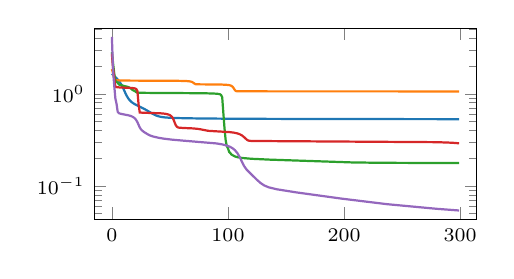
\begin{tikzpicture}

\definecolor{crimson2143940}{RGB}{214,39,40}
\definecolor{darkgray176}{RGB}{176,176,176}
\definecolor{darkorange25512714}{RGB}{255,127,14}
\definecolor{forestgreen4416044}{RGB}{44,160,44}
\definecolor{mediumpurple148103189}{RGB}{148,103,189}
\definecolor{steelblue31119180}{RGB}{31,119,180}

\begin{axis}[compar,
	ymode=log]
\addplot [thick, steelblue31119180]
table {%
0 1.65230560302734
1 1.60967218875885
3 1.51980757713318
5 1.4276807308197
6 1.37903583049774
7 1.32599353790283
8 1.26667380332947
9 1.20057117938995
11 1.05875587463379
12 0.993848085403442
13 0.939155459403992
14 0.895524501800537
15 0.861427426338196
16 0.834641695022583
17 0.813176393508911
18 0.795508742332458
19 0.780535697937012
21 0.755721092224121
24 0.724630355834961
28 0.684367299079895
32 0.640052795410156
35 0.6075519323349
37 0.589563608169556
39 0.575842380523682
41 0.56618332862854
43 0.559664726257324
46 0.553641200065613
50 0.549216270446777
57 0.545149207115173
70 0.541172504425049
93 0.53755521774292
135 0.534475564956665
221 0.531806707382202
299 0.530493259429932
};
\addplot [thick, darkorange25512714]
table {%
0 1.85211646556854
1 1.67770111560822
2 1.46272897720337
3 1.41593718528748
4 1.40484702587128
5 1.39981067180634
7 1.39501214027405
10 1.39188122749329
16 1.38930439949036
32 1.38671922683716
55 1.38247323036194
61 1.37871134281158
64 1.3742892742157
66 1.36830806732178
67 1.36319196224213
68 1.3552680015564
69 1.34236979484558
70 1.32132458686829
71 1.292635679245
72 1.27158439159393
73 1.26629757881165
76 1.26518905162811
89 1.26179456710815
95 1.25753927230835
98 1.25268864631653
100 1.24624443054199
101 1.24075663089752
102 1.23218429088593
103 1.21773552894592
104 1.191610455513
105 1.1454873085022
106 1.09121680259705
107 1.06940352916718
108 1.06570613384247
111 1.06433713436127
144 1.06147050857544
275 1.06137251853943
299 1.06136870384216
};
\addplot [thick, forestgreen4416044]
table {%
0 2.84194612503052
1 2.15506029129028
2 1.66873693466187
3 1.38294208049774
5 1.31623303890228
6 1.26444888114929
7 1.24834167957306
9 1.23046517372131
11 1.20998632907867
13 1.19424068927765
14 1.18405818939209
15 1.1702915430069
16 1.15001618862152
17 1.1210218667984
18 1.09569573402405
19 1.08197319507599
20 1.06478106975555
21 1.0405730009079
22 1.02683997154236
25 1.02437090873718
35 1.02164471149445
77 1.01418256759644
85 1.00862324237823
89 1.00375008583069
91 0.999232292175293
92 0.9952312707901
93 0.988119006156921
94 0.972235679626465
95 0.91933798789978
96 0.616937160491943
97 0.421802282333374
98 0.312908411026001
99 0.270792961120605
100 0.255544066429138
101 0.234020471572876
102 0.227557420730591
103 0.219099283218384
106 0.209146738052368
108 0.20545756816864
112 0.201385498046875
120 0.197391390800476
136 0.193149089813232
207 0.180134654045105
232 0.178421974182129
299 0.177336454391479
};
\addplot [thick, crimson2143940]
table {%
0 2.71224212646484
1 1.89663374423981
2 1.51032817363739
3 1.19073891639709
4 1.18067479133606
6 1.17347884178162
9 1.16805064678192
17 1.15556478500366
19 1.1488208770752
20 1.14171743392944
21 1.12556207180023
22 1.0690438747406
23 0.763562440872192
24 0.626803040504456
26 0.623935461044312
42 0.614003896713257
45 0.609050154685974
47 0.603470325469971
49 0.593772172927856
50 0.585844755172729
51 0.574084281921387
52 0.555935382843018
53 0.527923822402954
54 0.490156412124634
55 0.456605553627014
56 0.438905239105225
57 0.431463479995728
58 0.428577065467834
61 0.426207780838013
70 0.421022057533264
74 0.416285991668701
77 0.410333037376404
83 0.396579504013062
88 0.392909526824951
101 0.38445782661438
105 0.37907612323761
108 0.372137427330017
110 0.364766120910645
112 0.353622436523438
114 0.337481260299683
116 0.319562911987305
117 0.313272714614868
118 0.309869647026062
120 0.30800199508667
132 0.30707573890686
280 0.298706293106079
293 0.294538974761963
299 0.290218830108643
};
\addplot [thick, mediumpurple148103189]
table {%
0 4.13749027252197
1 1.78226494789124
2 1.23609900474548
3 0.890265941619873
4 0.779228687286377
5 0.638609528541565
6 0.617340087890625
7 0.609525799751282
9 0.601629018783569
14 0.585130453109741
16 0.575769901275635
17 0.569563150405884
18 0.561703205108643
19 0.551372528076172
20 0.537355184555054
21 0.517969131469727
22 0.491822361946106
23 0.46056592464447
24 0.431907415390015
25 0.412346363067627
26 0.399762630462646
28 0.382634878158569
31 0.362732648849487
33 0.35280454158783
36 0.34282374382019
40 0.333760499954224
45 0.325755834579468
52 0.317875027656555
63 0.309140682220459
90 0.289501667022705
95 0.28264594078064
99 0.274349570274353
102 0.264988541603088
104 0.256195902824402
106 0.244262218475342
108 0.227995634078979
110 0.206859588623047
113 0.172638773918152
114 0.163624286651611
116 0.150722026824951
119 0.13795006275177
125 0.116512775421143
128 0.107834815979004
131 0.10168719291687
135 0.0967668294906616
142 0.0921484231948853
159 0.0851820707321167
198 0.0729167461395264
237 0.0635035037994385
279 0.0566712617874146
299 0.0542340278625488
};
\end{axis}

\end{tikzpicture}
}
&
\multicolumn{4}{c}{% This file was created with tikzplotlib v0.10.1.
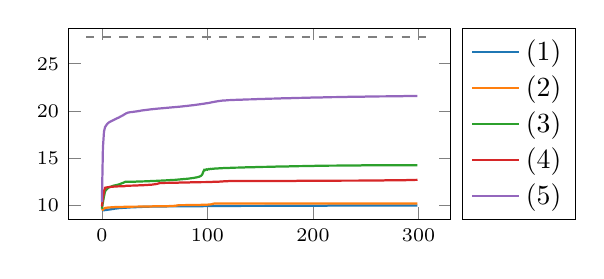
\begin{tikzpicture}

\definecolor{crimson2143940}{RGB}{214,39,40}
\definecolor{darkgray176}{RGB}{176,176,176}
\definecolor{darkorange25512714}{RGB}{255,127,14}
\definecolor{forestgreen4416044}{RGB}{44,160,44}
\definecolor{mediumpurple148103189}{RGB}{148,103,189}
\definecolor{steelblue31119180}{RGB}{31,119,180}

\begin{axis}[compar, legend pos=outer north east]
\addplot [thick, steelblue31119180]
table {%
0 9.43000030517578
1 9.44999980926514
3 9.47000026702881
4 9.48999977111816
5 9.5
6 9.52000045776367
7 9.52999973297119
9 9.56999969482422
10 9.57999992370605
13 9.64000034332275
15 9.65999984741211
16 9.68000030517578
18 9.69999980926514
19 9.69999980926514
22 9.72999954223633
23 9.72999954223633
25 9.75
26 9.75
27 9.76000022888184
28 9.76000022888184
29 9.77000045776367
30 9.77000045776367
31 9.77999973297119
32 9.77999973297119
34 9.80000019073486
35 9.80000019073486
36 9.8100004196167
38 9.8100004196167
39 9.81999969482422
40 9.81999969482422
41 9.82999992370605
44 9.82999992370605
45 9.84000015258789
48 9.84000015258789
49 9.85000038146973
54 9.85000038146973
55 9.85999965667725
61 9.85999965667725
62 9.86999988555908
71 9.86999988555908
72 9.88000011444092
82 9.88000011444092
83 9.89000034332275
96 9.89000034332275
97 9.89999961853027
112 9.89999961853027
113 9.90999984741211
131 9.90999984741211
132 9.92000007629395
154 9.92000007629395
155 9.93000030517578
181 9.93000030517578
182 9.9399995803833
213 9.9399995803833
214 9.94999980926514
251 9.94999980926514
252 9.96000003814697
295 9.96000003814697
296 9.97000026702881
299 9.97000026702881
};
\addlegendentry{$(1)$}
\addplot [thick, darkorange25512714]
table {%
0 9.4399995803833
1 9.52000045776367
2 9.64000034332275
3 9.6899995803833
4 9.72000026702881
5 9.72999954223633
6 9.75
7 9.76000022888184
8 9.76000022888184
10 9.77999973297119
11 9.77999973297119
12 9.78999996185303
14 9.78999996185303
15 9.80000019073486
16 9.80000019073486
17 9.8100004196167
20 9.8100004196167
21 9.81999969482422
24 9.81999969482422
25 9.82999992370605
29 9.82999992370605
30 9.84000015258789
34 9.84000015258789
35 9.85000038146973
40 9.85000038146973
41 9.85999965667725
47 9.85999965667725
48 9.86999988555908
53 9.86999988555908
54 9.88000011444092
59 9.88000011444092
60 9.89000034332275
63 9.89000034332275
64 9.89999961853027
66 9.89999961853027
70 9.9399995803833
72 9.97999954223633
74 10
79 10
80 10.0100002288818
87 10.0100002288818
88 10.0200004577637
93 10.0200004577637
94 10.0299997329712
97 10.0299997329712
98 10.039999961853
99 10.039999961853
103 10.0799999237061
104 10.1000003814697
106 10.1599998474121
107 10.1700000762939
170 10.1700000762939
171 10.1800003051758
299 10.1800003051758
};
\addlegendentry{$(2)$}
\addplot [thick, forestgreen4416044]
table {%
0 9.60999965667725
1 10.289999961853
2 10.9300003051758
3 11.4499998092651
4 11.6199998855591
5 11.710000038147
6 11.8199996948242
7 11.9099998474121
8 11.9399995803833
11 12.0600004196167
12 12.0900001525879
13 12.1099996566772
14 12.1400003433228
15 12.1599998474121
16 12.1899995803833
17 12.2299995422363
18 12.2799997329712
20 12.3599996566772
21 12.4099998474121
22 12.4700002670288
23 12.4799995422363
27 12.4799995422363
28 12.4899997711182
32 12.4899997711182
33 12.5
35 12.5
36 12.5100002288818
38 12.5100002288818
39 12.5200004577637
40 12.5200004577637
41 12.5299997329712
43 12.5299997329712
44 12.539999961853
45 12.539999961853
46 12.5500001907349
47 12.5500001907349
48 12.5600004196167
49 12.5600004196167
50 12.5699996948242
51 12.5699996948242
52 12.5799999237061
53 12.5799999237061
55 12.6000003814697
56 12.6000003814697
57 12.6099996566772
58 12.6099996566772
59 12.6199998855591
60 12.6199998855591
62 12.6400003433228
63 12.6400003433228
65 12.6599998474121
66 12.6599998474121
68 12.6800003051758
69 12.6800003051758
82 12.8100004196167
83 12.8299999237061
84 12.8400001525879
85 12.8599996566772
86 12.8699998855591
90 12.9499998092651
92 13.0100002288818
93 13.0500001907349
94 13.1199998855591
95 13.2299995422363
96 13.5100002288818
97 13.75
98 13.7200002670288
99 13.8000001907349
100 13.7600002288818
101 13.8299999237061
102 13.8100004196167
103 13.8500003814697
104 13.8400001525879
105 13.8699998855591
106 13.8599996566772
107 13.8800001144409
108 13.8800001144409
109 13.8900003433228
110 13.8900003433228
111 13.9099998474121
112 13.9099998474121
113 13.9200000762939
114 13.9200000762939
115 13.9300003051758
117 13.9300003051758
118 13.9399995803833
119 13.9399995803833
120 13.9499998092651
121 13.9499998092651
122 13.960000038147
124 13.960000038147
125 13.9700002670288
126 13.9700002670288
127 13.9799995422363
129 13.9799995422363
130 13.9899997711182
132 13.9899997711182
133 14
135 14
136 14.0100002288818
138 14.0100002288818
139 14.0200004577637
142 14.0200004577637
143 14.0299997329712
145 14.0299997329712
146 14.039999961853
149 14.039999961853
150 14.0500001907349
152 14.0500001907349
153 14.0600004196167
156 14.0600004196167
157 14.0699996948242
160 14.0699996948242
161 14.0799999237061
164 14.0799999237061
165 14.0900001525879
168 14.0900001525879
169 14.1000003814697
172 14.1000003814697
173 14.1099996566772
177 14.1099996566772
178 14.1199998855591
181 14.1199998855591
182 14.1300001144409
186 14.1300001144409
187 14.1400003433228
190 14.1400003433228
191 14.1499996185303
195 14.1499996185303
196 14.1599998474121
201 14.1599998474121
202 14.1700000762939
207 14.1700000762939
208 14.1800003051758
214 14.1800003051758
215 14.1899995803833
222 14.1899995803833
223 14.1999998092651
232 14.1999998092651
233 14.210000038147
245 14.210000038147
246 14.2200002670288
262 14.2200002670288
263 14.2299995422363
281 14.2299995422363
282 14.2399997711182
299 14.2399997711182
};
\addlegendentry{$(3)$}
\addplot [thick, crimson2143940]
table {%
0 9.85000038146973
1 10.7600002288818
2 11.4700002670288
3 11.8400001525879
4 11.8699998855591
5 11.8900003433228
6 11.8999996185303
7 11.9200000762939
12 11.9700002670288
13 11.9700002670288
15 11.9899997711182
16 11.9899997711182
17 12
18 12
19 12.0100002288818
21 12.0100002288818
22 12.0200004577637
23 12.0600004196167
27 12.0600004196167
28 12.0699996948242
29 12.0699996948242
30 12.0799999237061
32 12.0799999237061
33 12.0900001525879
34 12.0900001525879
35 12.1000003814697
36 12.1000003814697
37 12.1099996566772
38 12.1099996566772
39 12.1199998855591
40 12.1199998855591
42 12.1400003433228
43 12.1400003433228
45 12.1599998474121
46 12.1599998474121
48 12.1800003051758
49 12.1999998092651
50 12.210000038147
52 12.25
55 12.3400001525879
56 12.3500003814697
59 12.3500003814697
60 12.3599996566772
63 12.3599996566772
64 12.3699998855591
68 12.3699998855591
69 12.3800001144409
72 12.3800001144409
73 12.3900003433228
76 12.3900003433228
77 12.3999996185303
80 12.3999996185303
81 12.4099998474121
83 12.4099998474121
84 12.4200000762939
88 12.4200000762939
89 12.4300003051758
93 12.4300003051758
94 12.4399995803833
98 12.4399995803833
99 12.4499998092651
101 12.4499998092651
102 12.460000038147
104 12.460000038147
105 12.4700002670288
107 12.4700002670288
108 12.4799995422363
109 12.4799995422363
110 12.4899997711182
111 12.4899997711182
112 12.5
113 12.5
116 12.5299997329712
117 12.5299997329712
118 12.539999961853
119 12.539999961853
120 12.5500001907349
136 12.5500001907349
137 12.5600004196167
160 12.5600004196167
161 12.5699996948242
184 12.5699996948242
185 12.5799999237061
207 12.5799999237061
208 12.5900001525879
226 12.5900001525879
227 12.6000003814697
243 12.6000003814697
244 12.6099996566772
257 12.6099996566772
258 12.6199998855591
267 12.6199998855591
268 12.6300001144409
276 12.6300001144409
277 12.6400003433228
283 12.6400003433228
284 12.6499996185303
288 12.6499996185303
289 12.6599998474121
292 12.6599998474121
293 12.6700000762939
296 12.6700000762939
297 12.6800003051758
298 12.6800003051758
299 12.6899995803833
};
\addlegendentry{$(4)$}
\addplot [thick, mediumpurple148103189]
table {%
0 10.3500003814697
1 16.1200008392334
2 17.7999992370605
3 18.2800006866455
4 18.4400005340576
5 18.6100006103516
6 18.7099990844727
7 18.7999992370605
9 18.9200000762939
10 18.9699993133545
11 19.0300006866455
12 19.0799999237061
13 19.1399993896484
14 19.1900005340576
15 19.25
16 19.2900009155273
17 19.3600006103516
18 19.4099998474121
19 19.4799995422363
20 19.5300006866455
21 19.6100006103516
22 19.6700000762939
23 19.7399997711182
24 19.7800006866455
25 19.8299999237061
26 19.8400001525879
27 19.8700008392334
28 19.8700008392334
29 19.8899993896484
30 19.8999996185303
31 19.9200000762939
32 19.9300003051758
33 19.9500007629395
34 19.9599990844727
35 19.9899997711182
36 20
37 20.0300006866455
38 20.0400009155273
39 20.0599994659424
40 20.0699996948242
41 20.0900001525879
42 20.1000003814697
43 20.1200008392334
44 20.1299991607666
45 20.1499996185303
48 20.1800003051758
49 20.2000007629395
50 20.2000007629395
51 20.2199993133545
76 20.4699993133545
77 20.4899997711182
81 20.5300006866455
82 20.5499992370605
84 20.5699996948242
85 20.5900001525879
87 20.6100006103516
88 20.6299991607666
89 20.6399993896484
90 20.6599998474121
91 20.6700000762939
92 20.6900005340576
93 20.7000007629395
95 20.7399997711182
96 20.75
99 20.8099994659424
100 20.8199996948242
103 20.8799991607666
104 20.9099998474121
111 21.0499992370605
113 21.0699996948242
114 21.0900001525879
116 21.1100006103516
117 21.1100006103516
120 21.1399993896484
121 21.1399993896484
122 21.1499996185303
123 21.1499996185303
124 21.1599998474121
125 21.1599998474121
126 21.1700000762939
127 21.1700000762939
128 21.1800003051758
130 21.1800003051758
131 21.1900005340576
133 21.1900005340576
134 21.2000007629395
135 21.2000007629395
136 21.2099990844727
138 21.2099990844727
139 21.2199993133545
141 21.2199993133545
142 21.2299995422363
143 21.2299995422363
144 21.2399997711182
146 21.2399997711182
147 21.25
149 21.25
150 21.2600002288818
152 21.2600002288818
153 21.2700004577637
154 21.2700004577637
155 21.2800006866455
157 21.2800006866455
158 21.2900009155273
160 21.2900009155273
161 21.2999992370605
163 21.2999992370605
164 21.3099994659424
166 21.3099994659424
167 21.3199996948242
169 21.3199996948242
170 21.3299999237061
172 21.3299999237061
173 21.3400001525879
176 21.3400001525879
177 21.3500003814697
179 21.3500003814697
180 21.3600006103516
182 21.3600006103516
183 21.3700008392334
186 21.3700008392334
187 21.3799991607666
189 21.3799991607666
190 21.3899993896484
193 21.3899993896484
194 21.3999996185303
197 21.3999996185303
198 21.4099998474121
201 21.4099998474121
202 21.4200000762939
205 21.4200000762939
206 21.4300003051758
209 21.4300003051758
210 21.4400005340576
213 21.4400005340576
214 21.4500007629395
217 21.4500007629395
218 21.4599990844727
222 21.4599990844727
223 21.4699993133545
227 21.4699993133545
228 21.4799995422363
232 21.4799995422363
233 21.4899997711182
238 21.4899997711182
239 21.5
243 21.5
244 21.5100002288818
249 21.5100002288818
250 21.5200004577637
255 21.5200004577637
256 21.5300006866455
262 21.5300006866455
263 21.5400009155273
269 21.5400009155273
270 21.5499992370605
277 21.5499992370605
278 21.5599994659424
285 21.5599994659424
286 21.5699996948242
294 21.5699996948242
295 21.5799999237061
299 21.5799999237061
};
\addlegendentry{$(5)$}
\addplot [thick, gray, dashed]
table {%
-14.95 27.8502388000488
313.95 27.8502388000488
};
\end{axis}

\end{tikzpicture}
}
\end{tabular}
	\caption{Résultats de la LGD avec différents niveau de compression --- sans passe-bas}
	\label{fig:LGDsizes-s}
\end{figure}

\begin{figure}[H]\centering
	\begin{tabular}{c c c c c c}
Target  &  $(1)$  &  $(2)$  &  $(3)$  &  $(4)$

\\

\multirow{2}{0.3\textwidth}[0.125\textwidth]{\includegraphics[width=0.3\textwidth]{resultats/LGD/inits/inits-target-g.png}}
&
\includegraphics[width=0.15\textwidth]{resultats/LGD/inits/inits_1-init-pas=0.25_filtre=g-0.6.png}
&
\includegraphics[width=0.15\textwidth]{resultats/LGD/inits/inits_2-init-pas=0.25_filtre=g-0.6.png}
&
\includegraphics[width=0.15\textwidth]{resultats/LGD/inits/inits_3-init-pas=0.25_filtre=g-0.6.png}
&
\includegraphics[width=0.15\textwidth]{resultats/LGD/inits/inits_4-init-pas=0.25_filtre=g-0.6.png}

\\


&
\includegraphics[width=0.15\textwidth]{resultats/LGD/inits/inits_1-guess-pas=0.25_filtre=g-0.6.png}
&
\includegraphics[width=0.15\textwidth]{resultats/LGD/inits/inits_2-guess-pas=0.25_filtre=g-0.6.png}
&
\includegraphics[width=0.15\textwidth]{resultats/LGD/inits/inits_3-guess-pas=0.25_filtre=g-0.6.png}
&
\includegraphics[width=0.15\textwidth]{resultats/LGD/inits/inits_4-guess-pas=0.25_filtre=g-0.6.png}

\\ \\



\multicolumn{2}{c}{Loss}  &  \multicolumn{3}{c}{PSNR{\color{white}bbbb}}

\\

\multicolumn{2}{c}{% This file was created with tikzplotlib v0.10.1.
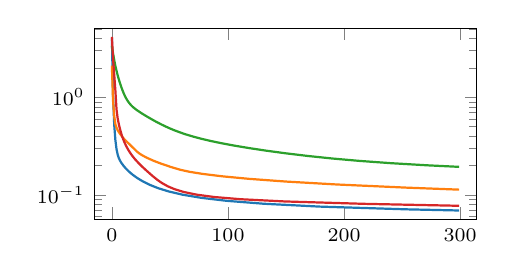
\begin{tikzpicture}

\definecolor{crimson2143940}{RGB}{214,39,40}
\definecolor{darkgray176}{RGB}{176,176,176}
\definecolor{darkorange25512714}{RGB}{255,127,14}
\definecolor{forestgreen4416044}{RGB}{44,160,44}
\definecolor{steelblue31119180}{RGB}{31,119,180}

\begin{axis}[compar,
	ymode=log]
\addplot [thick, steelblue31119180]
table {%
0 4.09705591201782
1 1.0397447347641
2 0.525999307632446
3 0.36544942855835
4 0.294240236282349
5 0.258731842041016
6 0.23837411403656
7 0.2248694896698
8 0.214669942855835
10 0.199013829231262
12 0.18678867816925
15 0.172265887260437
18 0.160792350769043
22 0.148674130439758
27 0.136995673179626
33 0.126390695571899
40 0.117159008979797
49 0.108532667160034
61 0.100532412528992
77 0.0933989286422729
99 0.0870349407196045
131 0.0812307596206665
179 0.0759825706481934
254 0.0712192058563232
299 0.0692975521087646
};
\addplot [thick, darkorange25512714]
table {%
0 2.11676383018494
1 0.9190913438797
2 0.643004417419434
3 0.532035350799561
4 0.487879872322083
5 0.460638880729675
6 0.440029859542847
7 0.422846078872681
9 0.393353462219238
11 0.368957042694092
13 0.349978923797607
22 0.275432348251343
24 0.264232397079468
27 0.25137186050415
31 0.237775444984436
36 0.22367525100708
42 0.210012912750244
51 0.193120121955872
59 0.180989027023315
67 0.172550797462463
78 0.164394378662109
95 0.155235648155212
118 0.146238088607788
150 0.137122750282288
194 0.127958059310913
254 0.118792176246643
299 0.113348960876465
};
\addplot [thick, forestgreen4416044]
table {%
0 3.37779760360718
1 2.81990122795105
2 2.4142701625824
3 2.10492038726807
4 1.86983335018158
5 1.67920529842377
6 1.52351367473602
7 1.3948290348053
8 1.2856605052948
9 1.19226157665253
10 1.11291658878326
11 1.04617238044739
12 0.990375518798828
13 0.94380521774292
14 0.904836654663086
15 0.872018575668335
16 0.844097495079041
17 0.820020079612732
18 0.798925280570984
19 0.780128955841064
21 0.747454047203064
23 0.719166994094849
25 0.693710803985596
28 0.659082055091858
31 0.627551555633545
34 0.598529100418091
38 0.563355803489685
42 0.532020330429077
46 0.504339337348938
50 0.480038523674011
54 0.458757042884827
59 0.435793519020081
64 0.416170716285706
70 0.396113634109497
77 0.376400947570801
85 0.357464551925659
94 0.339470624923706
105 0.320858478546143
118 0.30225658416748
133 0.284092664718628
150 0.266751885414124
169 0.250633358955383
190 0.236100435256958
213 0.223376154899597
240 0.211698055267334
272 0.201091408729553
299 0.194014668464661
};
\addplot [thick, crimson2143940]
table {%
0 4.15872049331665
1 2.48774647712708
2 1.71559143066406
3 1.18148231506348
4 0.74964714050293
5 0.606518745422363
6 0.529028296470642
7 0.472540497779846
8 0.428424477577209
9 0.393683195114136
10 0.365716695785522
11 0.342551231384277
12 0.322939038276672
13 0.306079387664795
14 0.291416645050049
16 0.267123222351074
18 0.247718811035156
20 0.231697797775269
23 0.211907505989075
26 0.195417284965515
30 0.176599979400635
35 0.156593918800354
39 0.143312335014343
43 0.132702112197876
48 0.12282931804657
54 0.114545702934265
62 0.10715639591217
73 0.100697159767151
88 0.0952965021133423
111 0.0903933048248291
149 0.0857839584350586
217 0.0811049938201904
299 0.0774440765380859
};

\end{axis}

\end{tikzpicture}
}
&
\multicolumn{3}{c}{% This file was created with tikzplotlib v0.10.1.
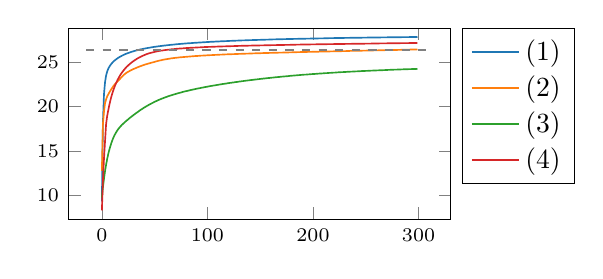
\begin{tikzpicture}

\definecolor{crimson2143940}{RGB}{214,39,40}
\definecolor{darkgray176}{RGB}{176,176,176}
\definecolor{darkorange25512714}{RGB}{255,127,14}
\definecolor{forestgreen4416044}{RGB}{44,160,44}
\definecolor{steelblue31119180}{RGB}{31,119,180}

\begin{axis}[compar, legend pos=outer north east]
\addplot [semithick, steelblue31119180]
table {%
0 9.34000015258789
1 18.2600002288818
2 21.3700008392334
3 22.7199993133545
4 23.4599990844727
5 23.8999996185303
6 24.2099990844727
7 24.4300003051758
8 24.6200008392334
9 24.7700004577637
10 24.9099998474121
11 25.0300006866455
12 25.1399993896484
15 25.4099998474121
16 25.4799995422363
17 25.5599994659424
21 25.7999992370605
24 25.9500007629395
29 26.1499996185303
30 26.1800003051758
31 26.2199993133545
37 26.3999996185303
38 26.4200000762939
39 26.4500007629395
41 26.4899997711182
42 26.5200004577637
50 26.6800003051758
51 26.6900005340576
53 26.7299995422363
54 26.7399997711182
55 26.7600002288818
56 26.7700004577637
57 26.7900009155273
58 26.7999992370605
59 26.8199996948242
61 26.8400001525879
62 26.8600006103516
64 26.8799991607666
65 26.8999996185303
69 26.9400005340576
70 26.9599990844727
82 27.0799999237061
83 27.0799999237061
88 27.1299991607666
89 27.1299991607666
93 27.1700000762939
94 27.1700000762939
96 27.1900005340576
97 27.1900005340576
100 27.2199993133545
101 27.2199993133545
103 27.2399997711182
104 27.2399997711182
105 27.25
106 27.25
108 27.2700004577637
109 27.2700004577637
110 27.2800006866455
111 27.2800006866455
113 27.2999992370605
114 27.2999992370605
115 27.3099994659424
116 27.3099994659424
117 27.3199996948242
118 27.3199996948242
119 27.3299999237061
120 27.3299999237061
121 27.3400001525879
122 27.3400001525879
123 27.3500003814697
124 27.3500003814697
125 27.3600006103516
126 27.3600006103516
127 27.3700008392334
128 27.3700008392334
129 27.3799991607666
130 27.3799991607666
131 27.3899993896484
132 27.3899993896484
133 27.3999996185303
135 27.3999996185303
136 27.4099998474121
137 27.4099998474121
138 27.4200000762939
139 27.4200000762939
140 27.4300003051758
142 27.4300003051758
143 27.4400005340576
144 27.4400005340576
145 27.4500007629395
147 27.4500007629395
148 27.4599990844727
150 27.4599990844727
151 27.4699993133545
153 27.4699993133545
154 27.4799995422363
155 27.4799995422363
156 27.4899997711182
158 27.4899997711182
159 27.5
161 27.5
162 27.5100002288818
164 27.5100002288818
165 27.5200004577637
168 27.5200004577637
169 27.5300006866455
171 27.5300006866455
172 27.5400009155273
174 27.5400009155273
175 27.5499992370605
178 27.5499992370605
179 27.5599994659424
181 27.5599994659424
182 27.5699996948242
185 27.5699996948242
186 27.5799999237061
189 27.5799999237061
190 27.5900001525879
193 27.5900001525879
194 27.6000003814697
197 27.6000003814697
198 27.6100006103516
201 27.6100006103516
202 27.6200008392334
205 27.6200008392334
206 27.6299991607666
210 27.6299991607666
211 27.6399993896484
214 27.6399993896484
215 27.6499996185303
219 27.6499996185303
220 27.6599998474121
224 27.6599998474121
225 27.6700000762939
229 27.6700000762939
230 27.6800003051758
234 27.6800003051758
235 27.6900005340576
240 27.6900005340576
241 27.7000007629395
246 27.7000007629395
247 27.7099990844727
251 27.7099990844727
252 27.7199993133545
257 27.7199993133545
258 27.7299995422363
264 27.7299995422363
265 27.7399997711182
270 27.7399997711182
271 27.75
277 27.75
278 27.7600002288818
284 27.7600002288818
285 27.7700004577637
291 27.7700004577637
292 27.7800006866455
298 27.7800006866455
299 27.7900009155273
};
\addlegendentry{$(1)$}
\addplot [semithick, darkorange25512714]
table {%
0 12.7600002288818
1 18.0300006866455
2 19.4099998474121
3 20.3700008392334
4 20.7800006866455
5 21.1100006103516
7 21.5499992370605
8 21.75
9 21.9400005340576
10 22.1200008392334
11 22.2900009155273
12 22.4400005340576
13 22.5799999237061
16 22.9400005340576
17 23.0699996948242
18 23.1900005340576
19 23.3199996948242
20 23.4400005340576
21 23.5499992370605
22 23.6499996185303
23 23.7399997711182
24 23.8199996948242
25 23.8899993896484
26 23.9500007629395
27 24.0200004577637
28 24.0799999237061
29 24.1299991607666
30 24.1900005340576
36 24.4899997711182
42 24.7299995422363
43 24.7600002288818
44 24.7999992370605
46 24.8600006103516
47 24.8999996185303
50 24.9899997711182
51 25.0300006866455
55 25.1499996185303
56 25.1700000762939
58 25.2299995422363
66 25.3899993896484
67 25.3999996185303
68 25.4200000762939
69 25.4300003051758
70 25.4500007629395
72 25.4699993133545
73 25.4899997711182
89 25.6499996185303
90 25.6499996185303
94 25.6900005340576
95 25.6900005340576
97 25.7099990844727
98 25.7099990844727
100 25.7299995422363
101 25.7299995422363
103 25.75
104 25.75
105 25.7600002288818
106 25.7600002288818
108 25.7800006866455
109 25.7800006866455
110 25.7900009155273
111 25.7900009155273
112 25.7999992370605
113 25.7999992370605
115 25.8199996948242
116 25.8199996948242
117 25.8299999237061
118 25.8299999237061
119 25.8400001525879
120 25.8400001525879
121 25.8500003814697
123 25.8500003814697
124 25.8600006103516
125 25.8600006103516
126 25.8700008392334
127 25.8700008392334
128 25.8799991607666
129 25.8799991607666
130 25.8899993896484
132 25.8899993896484
133 25.8999996185303
134 25.8999996185303
135 25.9099998474121
136 25.9099998474121
137 25.9200000762939
139 25.9200000762939
140 25.9300003051758
142 25.9300003051758
143 25.9400005340576
144 25.9400005340576
145 25.9500007629395
147 25.9500007629395
148 25.9599990844727
150 25.9599990844727
151 25.9699993133545
152 25.9699993133545
153 25.9799995422363
155 25.9799995422363
156 25.9899997711182
158 25.9899997711182
159 26
161 26
162 26.0100002288818
164 26.0100002288818
165 26.0200004577637
167 26.0200004577637
168 26.0300006866455
171 26.0300006866455
172 26.0400009155273
174 26.0400009155273
175 26.0499992370605
177 26.0499992370605
178 26.0599994659424
180 26.0599994659424
181 26.0699996948242
184 26.0699996948242
185 26.0799999237061
187 26.0799999237061
188 26.0900001525879
191 26.0900001525879
192 26.1000003814697
194 26.1000003814697
195 26.1100006103516
198 26.1100006103516
199 26.1200008392334
201 26.1200008392334
202 26.1299991607666
205 26.1299991607666
206 26.1399993896484
208 26.1399993896484
209 26.1499996185303
212 26.1499996185303
213 26.1599998474121
216 26.1599998474121
217 26.1700000762939
219 26.1700000762939
220 26.1800003051758
223 26.1800003051758
224 26.1900005340576
227 26.1900005340576
228 26.2000007629395
231 26.2000007629395
232 26.2099990844727
234 26.2099990844727
235 26.2199993133545
238 26.2199993133545
239 26.2299995422363
242 26.2299995422363
243 26.2399997711182
246 26.2399997711182
247 26.25
250 26.25
251 26.2600002288818
253 26.2600002288818
254 26.2700004577637
257 26.2700004577637
258 26.2800006866455
261 26.2800006866455
262 26.2900009155273
265 26.2900009155273
266 26.2999992370605
268 26.2999992370605
269 26.3099994659424
272 26.3099994659424
273 26.3199996948242
276 26.3199996948242
277 26.3299999237061
280 26.3299999237061
281 26.3400001525879
283 26.3400001525879
284 26.3500003814697
287 26.3500003814697
288 26.3600006103516
291 26.3600006103516
292 26.3700008392334
295 26.3700008392334
296 26.3799991607666
298 26.3799991607666
299 26.3899993896484
};
\addlegendentry{$(2)$}
\addplot [semithick, forestgreen4416044]
table {%
0 9.77999973297119
1 10.9300003051758
2 11.8999996185303
3 12.7399997711182
4 13.460000038147
5 14.0900001525879
6 14.6400003433228
7 15.1099996566772
8 15.5299997329712
9 15.8999996185303
10 16.2299995422363
11 16.5200004577637
12 16.7700004577637
13 16.9899997711182
14 17.1900005340576
15 17.3700008392334
16 17.5300006866455
17 17.6700000762939
19 17.9300003051758
22 18.2600002288818
27 18.7600002288818
32 19.2099990844727
33 19.2900009155273
34 19.3799991607666
35 19.4599990844727
36 19.5499992370605
37 19.6299991607666
38 19.7000007629395
40 19.8600006103516
45 20.2099990844727
51 20.5699996948242
52 20.6200008392334
53 20.6800003051758
57 20.8799991607666
58 20.9200000762939
59 20.9699993133545
61 21.0499992370605
62 21.1000003814697
65 21.2199993133545
66 21.25
68 21.3299999237061
69 21.3600006103516
70 21.3999996185303
71 21.4300003051758
72 21.4699993133545
75 21.5599994659424
76 21.6000003814697
79 21.6900005340576
80 21.7099990844727
84 21.8299999237061
85 21.8500003814697
87 21.9099998474121
88 21.9300003051758
89 21.9599990844727
90 21.9799995422363
91 22.0100002288818
93 22.0499992370605
94 22.0799999237061
96 22.1200008392334
97 22.1499996185303
100 22.2099990844727
101 22.2399997711182
115 22.5200004577637
116 22.5300006866455
121 22.6299991607666
122 22.6399993896484
124 22.6800003051758
125 22.6900005340576
127 22.7299995422363
128 22.7399997711182
130 22.7800006866455
131 22.7900009155273
133 22.8299999237061
134 22.8400001525879
135 22.8600006103516
136 22.8700008392334
137 22.8899993896484
138 22.8999996185303
139 22.9200000762939
140 22.9300003051758
141 22.9500007629395
142 22.9599990844727
143 22.9799995422363
144 22.9899997711182
145 23.0100002288818
147 23.0300006866455
148 23.0499992370605
149 23.0599994659424
150 23.0799999237061
152 23.1000003814697
153 23.1200008392334
155 23.1399993896484
156 23.1599998474121
159 23.1900005340576
160 23.2099990844727
163 23.2399997711182
164 23.2600002288818
168 23.2999992370605
169 23.3199996948242
177 23.3999996185303
178 23.4200000762939
192 23.5599994659424
193 23.5599994659424
201 23.6399993896484
202 23.6399993896484
207 23.6900005340576
208 23.6900005340576
212 23.7299995422363
213 23.7299995422363
216 23.7600002288818
217 23.7600002288818
220 23.7900009155273
221 23.7900009155273
224 23.8199996948242
225 23.8199996948242
227 23.8400001525879
228 23.8400001525879
230 23.8600006103516
231 23.8600006103516
233 23.8799991607666
234 23.8799991607666
236 23.8999996185303
237 23.8999996185303
238 23.9099998474121
239 23.9099998474121
241 23.9300003051758
242 23.9300003051758
243 23.9400005340576
244 23.9400005340576
246 23.9599990844727
247 23.9599990844727
248 23.9699993133545
249 23.9699993133545
250 23.9799995422363
251 23.9799995422363
253 24
254 24
255 24.0100002288818
256 24.0100002288818
257 24.0200004577637
258 24.0200004577637
259 24.0300006866455
260 24.0300006866455
261 24.0400009155273
262 24.0400009155273
263 24.0499992370605
264 24.0499992370605
265 24.0599994659424
266 24.0599994659424
267 24.0699996948242
268 24.0699996948242
269 24.0799999237061
270 24.0799999237061
271 24.0900001525879
272 24.0900001525879
273 24.1000003814697
274 24.1000003814697
275 24.1100006103516
276 24.1100006103516
277 24.1200008392334
279 24.1200008392334
280 24.1299991607666
281 24.1299991607666
282 24.1399993896484
283 24.1399993896484
284 24.1499996185303
285 24.1499996185303
286 24.1599998474121
288 24.1599998474121
289 24.1700000762939
290 24.1700000762939
291 24.1800003051758
293 24.1800003051758
294 24.1900005340576
295 24.1900005340576
296 24.2000007629395
298 24.2000007629395
299 24.2099990844727
};
\addlegendentry{$(3)$}
\addplot [semithick, crimson2143940]
table {%
0 8.32999992370605
1 11.6999998092651
2 14.1499996185303
3 16.1100006103516
4 18.0300006866455
5 18.9099998474121
6 19.5400009155273
7 20.1200008392334
8 20.6399993896484
9 21.1000003814697
10 21.5
11 21.8600006103516
12 22.1900005340576
13 22.4799995422363
14 22.75
15 23
16 23.2199993133545
17 23.4300003051758
18 23.6200008392334
19 23.7900009155273
20 23.9500007629395
21 24.1000003814697
22 24.2399997711182
23 24.3700008392334
24 24.4899997711182
26 24.7099990844727
28 24.9099998474121
29 25
30 25.0799999237061
31 25.1700000762939
32 25.2399997711182
33 25.3199996948242
35 25.4599990844727
38 25.6399993896484
42 25.8400001525879
45 25.9599990844727
51 26.1399993896484
53 26.1800003051758
54 26.2099990844727
56 26.25
57 26.2600002288818
60 26.3199996948242
61 26.3299999237061
62 26.3500003814697
64 26.3700008392334
65 26.3899993896484
69 26.4300003051758
70 26.4500007629395
74 26.4899997711182
75 26.4899997711182
80 26.5400009155273
81 26.5400009155273
84 26.5699996948242
85 26.5699996948242
87 26.5900001525879
88 26.5900001525879
90 26.6100006103516
91 26.6100006103516
92 26.6200008392334
93 26.6200008392334
94 26.6299991607666
95 26.6299991607666
97 26.6499996185303
98 26.6499996185303
99 26.6599998474121
100 26.6599998474121
101 26.6700000762939
103 26.6700000762939
104 26.6800003051758
105 26.6800003051758
106 26.6900005340576
107 26.6900005340576
108 26.7000007629395
109 26.7000007629395
110 26.7099990844727
112 26.7099990844727
113 26.7199993133545
114 26.7199993133545
115 26.7299995422363
117 26.7299995422363
118 26.7399997711182
120 26.7399997711182
121 26.75
122 26.75
123 26.7600002288818
125 26.7600002288818
126 26.7700004577637
128 26.7700004577637
129 26.7800006866455
131 26.7800006866455
132 26.7900009155273
135 26.7900009155273
136 26.7999992370605
138 26.7999992370605
139 26.8099994659424
141 26.8099994659424
142 26.8199996948242
145 26.8199996948242
146 26.8299999237061
149 26.8299999237061
150 26.8400001525879
153 26.8400001525879
154 26.8500003814697
156 26.8500003814697
157 26.8600006103516
160 26.8600006103516
161 26.8700008392334
165 26.8700008392334
166 26.8799991607666
169 26.8799991607666
170 26.8899993896484
173 26.8899993896484
174 26.8999996185303
178 26.8999996185303
179 26.9099998474121
183 26.9099998474121
184 26.9200000762939
187 26.9200000762939
188 26.9300003051758
192 26.9300003051758
193 26.9400005340576
197 26.9400005340576
198 26.9500007629395
202 26.9500007629395
203 26.9599990844727
208 26.9599990844727
209 26.9699993133545
213 26.9699993133545
214 26.9799995422363
219 26.9799995422363
220 26.9899997711182
225 26.9899997711182
226 27
230 27
231 27.0100002288818
236 27.0100002288818
237 27.0200004577637
243 27.0200004577637
244 27.0300006866455
249 27.0300006866455
250 27.0400009155273
255 27.0400009155273
256 27.0499992370605
262 27.0499992370605
263 27.0599994659424
269 27.0599994659424
270 27.0699996948242
275 27.0699996948242
276 27.0799999237061
282 27.0799999237061
283 27.0900001525879
290 27.0900001525879
291 27.1000003814697
297 27.1000003814697
298 27.1100006103516
299 27.1100006103516
};
\addlegendentry{$(4)$}
\addplot [semithick, gray,  dashed]
table {%
-14.95 26.3238544464111
313.95 26.3238544464111
};
\end{axis}

\end{tikzpicture}
}
\end{tabular}
	\caption{Idem, cette fois avec un passe-bas gaussien ($\sigma=0.5$)}
	\label{fig:LGDsizes-g}
\end{figure}


\vfill



\subsection{Variation de la taille de l'espace latent}\label{sec:LGDlat}

Toujours dans l'optique de voir les limites de la méthode, trois autres auto-encodeurs ont été entraînés avec différentes tailles d'espace latent. Pour chacun --- \textit{fig. \ref{fig:LGDlat100-s}} à \textit{ \ref{fig:LGDlat800-g}} --- la LGD est effectuée avec différentes initialisations (toujours en première ligne avec la prédiction en dessous). En fonction des cas, la loss fait parfois des zig-zags, ce qui indique que le pas est trop grand. Mais même sachant cela, les résultats sont étonnamment bons. En particulier pour les deux dernières figures, où $d=800$ ce qui est plus que la taille des images, à savoir $28\times28=784$. \`A noter tout de même qu'à mesure que $d$ augmente les PSNR reste de plus en plus loin du PSNR de référence (PSNR$(\bf{x_0}, f(\bf{x_0}))$), qui lui reste globalement stable d'un auto-encodeur à l'autre.
\\
On y voit aussi qu'à mesure que $d$ augmente, les cas sans passe-bas présentent de moins en moins de plateaux, là où avec, on commence à voir apparaître des sauts, peut-être également dû au pas trop grand.

\vfill

\newpage

\begin{figure}[H]\centering
	\begin{tabular}{c c c c c c}
Target  &  $(1)$  &  $(2)$  &  $(3)$  &  $(4)$  &  $(5)$

\\

\multirow{3}{0.3\textwidth}[0.05\textwidth]{\includegraphics[width=0.3\textwidth]{resultats/LGD/sizes/size-target-s.png}}
&
\includegraphics[width=0.12\textwidth]{resultats/LGD/sizes/size_big-init-pas=0.1_filtre=s-None.png}
&
\includegraphics[width=0.12\textwidth]{resultats/LGD/sizes/size_mid2-init-pas=0.1_filtre=s-None.png}
&
\includegraphics[width=0.12\textwidth]{resultats/LGD/sizes/size_mid1-init-pas=0.1_filtre=s-None.png}
&
\includegraphics[width=0.12\textwidth]{resultats/LGD/sizes/size_small-init-pas=0.05_filtre=s-None.png}
&
\includegraphics[width=0.12\textwidth]{resultats/LGD/sizes/size_mini-init-pas=0.01_filtre=s-None.png}

\\


&
\includegraphics[width=0.12\textwidth]{resultats/LGD/sizes/size_big-compatarget-s.png}
&
\includegraphics[width=0.12\textwidth]{resultats/LGD/sizes/size_mid2-compatarget-s.png}
&
\includegraphics[height=0.12\textwidth]{resultats/LGD/sizes/size_mid1-compatarget-s.png}
&
\includegraphics[width=0.12\textwidth]{resultats/LGD/sizes/size_small-compatarget-s.png}
&
\includegraphics[width=0.12\textwidth]{resultats/LGD/sizes/size_mini-compatarget-s.png}

\\


&
\includegraphics[width=0.12\textwidth]{resultats/LGD/sizes/size_big-guess-pas=0.1_filtre=s-None.png}
&
\includegraphics[width=0.12\textwidth]{resultats/LGD/sizes/size_mid2-guess-pas=0.1_filtre=s-None.png}
&
\includegraphics[width=0.12\textwidth]{resultats/LGD/sizes/size_mid1-guess-pas=0.1_filtre=s-None.png}
&
\includegraphics[width=0.12\textwidth]{resultats/LGD/sizes/size_small-guess-pas=0.05_filtre=s-None.png}
&
\includegraphics[width=0.12\textwidth]{resultats/LGD/sizes/size_mini-guess-pas=0.01_filtre=s-None.png}

\\ \\



\multicolumn{2}{c}{Loss}  &  \multicolumn{4}{c}{PSNR{\color{white}bbbb}}

\\

\multicolumn{2}{c}{% This file was created with tikzplotlib v0.10.1.
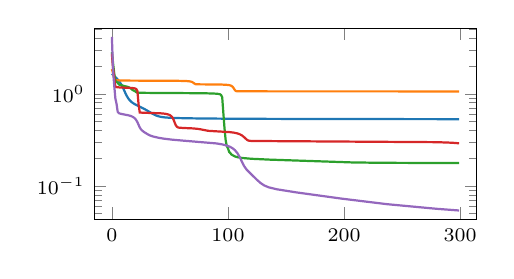
\begin{tikzpicture}

\definecolor{crimson2143940}{RGB}{214,39,40}
\definecolor{darkgray176}{RGB}{176,176,176}
\definecolor{darkorange25512714}{RGB}{255,127,14}
\definecolor{forestgreen4416044}{RGB}{44,160,44}
\definecolor{mediumpurple148103189}{RGB}{148,103,189}
\definecolor{steelblue31119180}{RGB}{31,119,180}

\begin{axis}[compar,
	ymode=log]
\addplot [thick, steelblue31119180]
table {%
0 1.65230560302734
1 1.60967218875885
3 1.51980757713318
5 1.4276807308197
6 1.37903583049774
7 1.32599353790283
8 1.26667380332947
9 1.20057117938995
11 1.05875587463379
12 0.993848085403442
13 0.939155459403992
14 0.895524501800537
15 0.861427426338196
16 0.834641695022583
17 0.813176393508911
18 0.795508742332458
19 0.780535697937012
21 0.755721092224121
24 0.724630355834961
28 0.684367299079895
32 0.640052795410156
35 0.6075519323349
37 0.589563608169556
39 0.575842380523682
41 0.56618332862854
43 0.559664726257324
46 0.553641200065613
50 0.549216270446777
57 0.545149207115173
70 0.541172504425049
93 0.53755521774292
135 0.534475564956665
221 0.531806707382202
299 0.530493259429932
};
\addplot [thick, darkorange25512714]
table {%
0 1.85211646556854
1 1.67770111560822
2 1.46272897720337
3 1.41593718528748
4 1.40484702587128
5 1.39981067180634
7 1.39501214027405
10 1.39188122749329
16 1.38930439949036
32 1.38671922683716
55 1.38247323036194
61 1.37871134281158
64 1.3742892742157
66 1.36830806732178
67 1.36319196224213
68 1.3552680015564
69 1.34236979484558
70 1.32132458686829
71 1.292635679245
72 1.27158439159393
73 1.26629757881165
76 1.26518905162811
89 1.26179456710815
95 1.25753927230835
98 1.25268864631653
100 1.24624443054199
101 1.24075663089752
102 1.23218429088593
103 1.21773552894592
104 1.191610455513
105 1.1454873085022
106 1.09121680259705
107 1.06940352916718
108 1.06570613384247
111 1.06433713436127
144 1.06147050857544
275 1.06137251853943
299 1.06136870384216
};
\addplot [thick, forestgreen4416044]
table {%
0 2.84194612503052
1 2.15506029129028
2 1.66873693466187
3 1.38294208049774
5 1.31623303890228
6 1.26444888114929
7 1.24834167957306
9 1.23046517372131
11 1.20998632907867
13 1.19424068927765
14 1.18405818939209
15 1.1702915430069
16 1.15001618862152
17 1.1210218667984
18 1.09569573402405
19 1.08197319507599
20 1.06478106975555
21 1.0405730009079
22 1.02683997154236
25 1.02437090873718
35 1.02164471149445
77 1.01418256759644
85 1.00862324237823
89 1.00375008583069
91 0.999232292175293
92 0.9952312707901
93 0.988119006156921
94 0.972235679626465
95 0.91933798789978
96 0.616937160491943
97 0.421802282333374
98 0.312908411026001
99 0.270792961120605
100 0.255544066429138
101 0.234020471572876
102 0.227557420730591
103 0.219099283218384
106 0.209146738052368
108 0.20545756816864
112 0.201385498046875
120 0.197391390800476
136 0.193149089813232
207 0.180134654045105
232 0.178421974182129
299 0.177336454391479
};
\addplot [thick, crimson2143940]
table {%
0 2.71224212646484
1 1.89663374423981
2 1.51032817363739
3 1.19073891639709
4 1.18067479133606
6 1.17347884178162
9 1.16805064678192
17 1.15556478500366
19 1.1488208770752
20 1.14171743392944
21 1.12556207180023
22 1.0690438747406
23 0.763562440872192
24 0.626803040504456
26 0.623935461044312
42 0.614003896713257
45 0.609050154685974
47 0.603470325469971
49 0.593772172927856
50 0.585844755172729
51 0.574084281921387
52 0.555935382843018
53 0.527923822402954
54 0.490156412124634
55 0.456605553627014
56 0.438905239105225
57 0.431463479995728
58 0.428577065467834
61 0.426207780838013
70 0.421022057533264
74 0.416285991668701
77 0.410333037376404
83 0.396579504013062
88 0.392909526824951
101 0.38445782661438
105 0.37907612323761
108 0.372137427330017
110 0.364766120910645
112 0.353622436523438
114 0.337481260299683
116 0.319562911987305
117 0.313272714614868
118 0.309869647026062
120 0.30800199508667
132 0.30707573890686
280 0.298706293106079
293 0.294538974761963
299 0.290218830108643
};
\addplot [thick, mediumpurple148103189]
table {%
0 4.13749027252197
1 1.78226494789124
2 1.23609900474548
3 0.890265941619873
4 0.779228687286377
5 0.638609528541565
6 0.617340087890625
7 0.609525799751282
9 0.601629018783569
14 0.585130453109741
16 0.575769901275635
17 0.569563150405884
18 0.561703205108643
19 0.551372528076172
20 0.537355184555054
21 0.517969131469727
22 0.491822361946106
23 0.46056592464447
24 0.431907415390015
25 0.412346363067627
26 0.399762630462646
28 0.382634878158569
31 0.362732648849487
33 0.35280454158783
36 0.34282374382019
40 0.333760499954224
45 0.325755834579468
52 0.317875027656555
63 0.309140682220459
90 0.289501667022705
95 0.28264594078064
99 0.274349570274353
102 0.264988541603088
104 0.256195902824402
106 0.244262218475342
108 0.227995634078979
110 0.206859588623047
113 0.172638773918152
114 0.163624286651611
116 0.150722026824951
119 0.13795006275177
125 0.116512775421143
128 0.107834815979004
131 0.10168719291687
135 0.0967668294906616
142 0.0921484231948853
159 0.0851820707321167
198 0.0729167461395264
237 0.0635035037994385
279 0.0566712617874146
299 0.0542340278625488
};
\end{axis}

\end{tikzpicture}
}
&
\multicolumn{4}{c}{% This file was created with tikzplotlib v0.10.1.
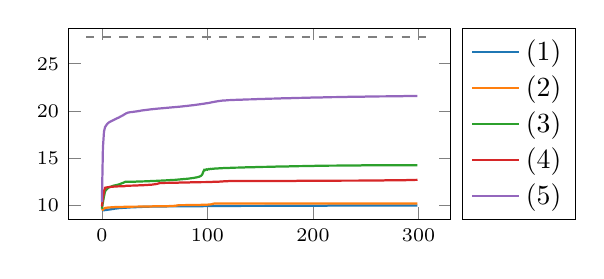
\begin{tikzpicture}

\definecolor{crimson2143940}{RGB}{214,39,40}
\definecolor{darkgray176}{RGB}{176,176,176}
\definecolor{darkorange25512714}{RGB}{255,127,14}
\definecolor{forestgreen4416044}{RGB}{44,160,44}
\definecolor{mediumpurple148103189}{RGB}{148,103,189}
\definecolor{steelblue31119180}{RGB}{31,119,180}

\begin{axis}[compar, legend pos=outer north east]
\addplot [thick, steelblue31119180]
table {%
0 9.43000030517578
1 9.44999980926514
3 9.47000026702881
4 9.48999977111816
5 9.5
6 9.52000045776367
7 9.52999973297119
9 9.56999969482422
10 9.57999992370605
13 9.64000034332275
15 9.65999984741211
16 9.68000030517578
18 9.69999980926514
19 9.69999980926514
22 9.72999954223633
23 9.72999954223633
25 9.75
26 9.75
27 9.76000022888184
28 9.76000022888184
29 9.77000045776367
30 9.77000045776367
31 9.77999973297119
32 9.77999973297119
34 9.80000019073486
35 9.80000019073486
36 9.8100004196167
38 9.8100004196167
39 9.81999969482422
40 9.81999969482422
41 9.82999992370605
44 9.82999992370605
45 9.84000015258789
48 9.84000015258789
49 9.85000038146973
54 9.85000038146973
55 9.85999965667725
61 9.85999965667725
62 9.86999988555908
71 9.86999988555908
72 9.88000011444092
82 9.88000011444092
83 9.89000034332275
96 9.89000034332275
97 9.89999961853027
112 9.89999961853027
113 9.90999984741211
131 9.90999984741211
132 9.92000007629395
154 9.92000007629395
155 9.93000030517578
181 9.93000030517578
182 9.9399995803833
213 9.9399995803833
214 9.94999980926514
251 9.94999980926514
252 9.96000003814697
295 9.96000003814697
296 9.97000026702881
299 9.97000026702881
};
\addlegendentry{$(1)$}
\addplot [thick, darkorange25512714]
table {%
0 9.4399995803833
1 9.52000045776367
2 9.64000034332275
3 9.6899995803833
4 9.72000026702881
5 9.72999954223633
6 9.75
7 9.76000022888184
8 9.76000022888184
10 9.77999973297119
11 9.77999973297119
12 9.78999996185303
14 9.78999996185303
15 9.80000019073486
16 9.80000019073486
17 9.8100004196167
20 9.8100004196167
21 9.81999969482422
24 9.81999969482422
25 9.82999992370605
29 9.82999992370605
30 9.84000015258789
34 9.84000015258789
35 9.85000038146973
40 9.85000038146973
41 9.85999965667725
47 9.85999965667725
48 9.86999988555908
53 9.86999988555908
54 9.88000011444092
59 9.88000011444092
60 9.89000034332275
63 9.89000034332275
64 9.89999961853027
66 9.89999961853027
70 9.9399995803833
72 9.97999954223633
74 10
79 10
80 10.0100002288818
87 10.0100002288818
88 10.0200004577637
93 10.0200004577637
94 10.0299997329712
97 10.0299997329712
98 10.039999961853
99 10.039999961853
103 10.0799999237061
104 10.1000003814697
106 10.1599998474121
107 10.1700000762939
170 10.1700000762939
171 10.1800003051758
299 10.1800003051758
};
\addlegendentry{$(2)$}
\addplot [thick, forestgreen4416044]
table {%
0 9.60999965667725
1 10.289999961853
2 10.9300003051758
3 11.4499998092651
4 11.6199998855591
5 11.710000038147
6 11.8199996948242
7 11.9099998474121
8 11.9399995803833
11 12.0600004196167
12 12.0900001525879
13 12.1099996566772
14 12.1400003433228
15 12.1599998474121
16 12.1899995803833
17 12.2299995422363
18 12.2799997329712
20 12.3599996566772
21 12.4099998474121
22 12.4700002670288
23 12.4799995422363
27 12.4799995422363
28 12.4899997711182
32 12.4899997711182
33 12.5
35 12.5
36 12.5100002288818
38 12.5100002288818
39 12.5200004577637
40 12.5200004577637
41 12.5299997329712
43 12.5299997329712
44 12.539999961853
45 12.539999961853
46 12.5500001907349
47 12.5500001907349
48 12.5600004196167
49 12.5600004196167
50 12.5699996948242
51 12.5699996948242
52 12.5799999237061
53 12.5799999237061
55 12.6000003814697
56 12.6000003814697
57 12.6099996566772
58 12.6099996566772
59 12.6199998855591
60 12.6199998855591
62 12.6400003433228
63 12.6400003433228
65 12.6599998474121
66 12.6599998474121
68 12.6800003051758
69 12.6800003051758
82 12.8100004196167
83 12.8299999237061
84 12.8400001525879
85 12.8599996566772
86 12.8699998855591
90 12.9499998092651
92 13.0100002288818
93 13.0500001907349
94 13.1199998855591
95 13.2299995422363
96 13.5100002288818
97 13.75
98 13.7200002670288
99 13.8000001907349
100 13.7600002288818
101 13.8299999237061
102 13.8100004196167
103 13.8500003814697
104 13.8400001525879
105 13.8699998855591
106 13.8599996566772
107 13.8800001144409
108 13.8800001144409
109 13.8900003433228
110 13.8900003433228
111 13.9099998474121
112 13.9099998474121
113 13.9200000762939
114 13.9200000762939
115 13.9300003051758
117 13.9300003051758
118 13.9399995803833
119 13.9399995803833
120 13.9499998092651
121 13.9499998092651
122 13.960000038147
124 13.960000038147
125 13.9700002670288
126 13.9700002670288
127 13.9799995422363
129 13.9799995422363
130 13.9899997711182
132 13.9899997711182
133 14
135 14
136 14.0100002288818
138 14.0100002288818
139 14.0200004577637
142 14.0200004577637
143 14.0299997329712
145 14.0299997329712
146 14.039999961853
149 14.039999961853
150 14.0500001907349
152 14.0500001907349
153 14.0600004196167
156 14.0600004196167
157 14.0699996948242
160 14.0699996948242
161 14.0799999237061
164 14.0799999237061
165 14.0900001525879
168 14.0900001525879
169 14.1000003814697
172 14.1000003814697
173 14.1099996566772
177 14.1099996566772
178 14.1199998855591
181 14.1199998855591
182 14.1300001144409
186 14.1300001144409
187 14.1400003433228
190 14.1400003433228
191 14.1499996185303
195 14.1499996185303
196 14.1599998474121
201 14.1599998474121
202 14.1700000762939
207 14.1700000762939
208 14.1800003051758
214 14.1800003051758
215 14.1899995803833
222 14.1899995803833
223 14.1999998092651
232 14.1999998092651
233 14.210000038147
245 14.210000038147
246 14.2200002670288
262 14.2200002670288
263 14.2299995422363
281 14.2299995422363
282 14.2399997711182
299 14.2399997711182
};
\addlegendentry{$(3)$}
\addplot [thick, crimson2143940]
table {%
0 9.85000038146973
1 10.7600002288818
2 11.4700002670288
3 11.8400001525879
4 11.8699998855591
5 11.8900003433228
6 11.8999996185303
7 11.9200000762939
12 11.9700002670288
13 11.9700002670288
15 11.9899997711182
16 11.9899997711182
17 12
18 12
19 12.0100002288818
21 12.0100002288818
22 12.0200004577637
23 12.0600004196167
27 12.0600004196167
28 12.0699996948242
29 12.0699996948242
30 12.0799999237061
32 12.0799999237061
33 12.0900001525879
34 12.0900001525879
35 12.1000003814697
36 12.1000003814697
37 12.1099996566772
38 12.1099996566772
39 12.1199998855591
40 12.1199998855591
42 12.1400003433228
43 12.1400003433228
45 12.1599998474121
46 12.1599998474121
48 12.1800003051758
49 12.1999998092651
50 12.210000038147
52 12.25
55 12.3400001525879
56 12.3500003814697
59 12.3500003814697
60 12.3599996566772
63 12.3599996566772
64 12.3699998855591
68 12.3699998855591
69 12.3800001144409
72 12.3800001144409
73 12.3900003433228
76 12.3900003433228
77 12.3999996185303
80 12.3999996185303
81 12.4099998474121
83 12.4099998474121
84 12.4200000762939
88 12.4200000762939
89 12.4300003051758
93 12.4300003051758
94 12.4399995803833
98 12.4399995803833
99 12.4499998092651
101 12.4499998092651
102 12.460000038147
104 12.460000038147
105 12.4700002670288
107 12.4700002670288
108 12.4799995422363
109 12.4799995422363
110 12.4899997711182
111 12.4899997711182
112 12.5
113 12.5
116 12.5299997329712
117 12.5299997329712
118 12.539999961853
119 12.539999961853
120 12.5500001907349
136 12.5500001907349
137 12.5600004196167
160 12.5600004196167
161 12.5699996948242
184 12.5699996948242
185 12.5799999237061
207 12.5799999237061
208 12.5900001525879
226 12.5900001525879
227 12.6000003814697
243 12.6000003814697
244 12.6099996566772
257 12.6099996566772
258 12.6199998855591
267 12.6199998855591
268 12.6300001144409
276 12.6300001144409
277 12.6400003433228
283 12.6400003433228
284 12.6499996185303
288 12.6499996185303
289 12.6599998474121
292 12.6599998474121
293 12.6700000762939
296 12.6700000762939
297 12.6800003051758
298 12.6800003051758
299 12.6899995803833
};
\addlegendentry{$(4)$}
\addplot [thick, mediumpurple148103189]
table {%
0 10.3500003814697
1 16.1200008392334
2 17.7999992370605
3 18.2800006866455
4 18.4400005340576
5 18.6100006103516
6 18.7099990844727
7 18.7999992370605
9 18.9200000762939
10 18.9699993133545
11 19.0300006866455
12 19.0799999237061
13 19.1399993896484
14 19.1900005340576
15 19.25
16 19.2900009155273
17 19.3600006103516
18 19.4099998474121
19 19.4799995422363
20 19.5300006866455
21 19.6100006103516
22 19.6700000762939
23 19.7399997711182
24 19.7800006866455
25 19.8299999237061
26 19.8400001525879
27 19.8700008392334
28 19.8700008392334
29 19.8899993896484
30 19.8999996185303
31 19.9200000762939
32 19.9300003051758
33 19.9500007629395
34 19.9599990844727
35 19.9899997711182
36 20
37 20.0300006866455
38 20.0400009155273
39 20.0599994659424
40 20.0699996948242
41 20.0900001525879
42 20.1000003814697
43 20.1200008392334
44 20.1299991607666
45 20.1499996185303
48 20.1800003051758
49 20.2000007629395
50 20.2000007629395
51 20.2199993133545
76 20.4699993133545
77 20.4899997711182
81 20.5300006866455
82 20.5499992370605
84 20.5699996948242
85 20.5900001525879
87 20.6100006103516
88 20.6299991607666
89 20.6399993896484
90 20.6599998474121
91 20.6700000762939
92 20.6900005340576
93 20.7000007629395
95 20.7399997711182
96 20.75
99 20.8099994659424
100 20.8199996948242
103 20.8799991607666
104 20.9099998474121
111 21.0499992370605
113 21.0699996948242
114 21.0900001525879
116 21.1100006103516
117 21.1100006103516
120 21.1399993896484
121 21.1399993896484
122 21.1499996185303
123 21.1499996185303
124 21.1599998474121
125 21.1599998474121
126 21.1700000762939
127 21.1700000762939
128 21.1800003051758
130 21.1800003051758
131 21.1900005340576
133 21.1900005340576
134 21.2000007629395
135 21.2000007629395
136 21.2099990844727
138 21.2099990844727
139 21.2199993133545
141 21.2199993133545
142 21.2299995422363
143 21.2299995422363
144 21.2399997711182
146 21.2399997711182
147 21.25
149 21.25
150 21.2600002288818
152 21.2600002288818
153 21.2700004577637
154 21.2700004577637
155 21.2800006866455
157 21.2800006866455
158 21.2900009155273
160 21.2900009155273
161 21.2999992370605
163 21.2999992370605
164 21.3099994659424
166 21.3099994659424
167 21.3199996948242
169 21.3199996948242
170 21.3299999237061
172 21.3299999237061
173 21.3400001525879
176 21.3400001525879
177 21.3500003814697
179 21.3500003814697
180 21.3600006103516
182 21.3600006103516
183 21.3700008392334
186 21.3700008392334
187 21.3799991607666
189 21.3799991607666
190 21.3899993896484
193 21.3899993896484
194 21.3999996185303
197 21.3999996185303
198 21.4099998474121
201 21.4099998474121
202 21.4200000762939
205 21.4200000762939
206 21.4300003051758
209 21.4300003051758
210 21.4400005340576
213 21.4400005340576
214 21.4500007629395
217 21.4500007629395
218 21.4599990844727
222 21.4599990844727
223 21.4699993133545
227 21.4699993133545
228 21.4799995422363
232 21.4799995422363
233 21.4899997711182
238 21.4899997711182
239 21.5
243 21.5
244 21.5100002288818
249 21.5100002288818
250 21.5200004577637
255 21.5200004577637
256 21.5300006866455
262 21.5300006866455
263 21.5400009155273
269 21.5400009155273
270 21.5499992370605
277 21.5499992370605
278 21.5599994659424
285 21.5599994659424
286 21.5699996948242
294 21.5699996948242
295 21.5799999237061
299 21.5799999237061
};
\addlegendentry{$(5)$}
\addplot [thick, gray, dashed]
table {%
-14.95 27.8502388000488
313.95 27.8502388000488
};
\end{axis}

\end{tikzpicture}
}
\end{tabular}
	\caption{$d=100$, sans passe-base}
	\label{fig:LGDlat100-s}
\end{figure}

\begin{figure}[H]\centering
	\begin{tabular}{c c c c c c}
	Target  &  $(1)$  &  $(2)$  &  $(3)$   &  $(4)$ &  $(5)$
	
	\\
	
	\multirow{2}{0.25\textwidth}[0.1\textwidth]{\includegraphics[width=0.25\textwidth]{resultats/LGD/lats/lat-100-target-g.png}}
	&
	\includegraphics[width=0.12\textwidth]{resultats/LGD/lats/lat-100_1-init-pas=0.25_filtre=g-0.6.png}
	&
	\includegraphics[width=0.12\textwidth]{resultats/LGD/lats/lat-100_2-init-pas=0.25_filtre=g-0.6.png}
	&
	\includegraphics[width=0.12\textwidth]{resultats/LGD/lats/lat-100_3-init-pas=0.25_filtre=g-0.6.png}
	&
	\includegraphics[width=0.12\textwidth]{resultats/LGD/lats/lat-100_4-init-pas=0.25_filtre=g-0.6.png}
	&
	\includegraphics[width=0.12\textwidth]{resultats/LGD/lats/lat-100_5-init-pas=0.25_filtre=g-0.6.png}
	
	\\
	
	
	&
	\includegraphics[width=0.12\textwidth]{resultats/LGD/lats/lat-100_1-guess-pas=0.25_filtre=g-0.6.png}
	&
	\includegraphics[width=0.12\textwidth]{resultats/LGD/lats/lat-100_2-guess-pas=0.25_filtre=g-0.6.png}
	&
	\includegraphics[width=0.12\textwidth]{resultats/LGD/lats/lat-100_3-guess-pas=0.25_filtre=g-0.6.png}
	&
	\includegraphics[width=0.12\textwidth]{resultats/LGD/lats/lat-100_4-guess-pas=0.25_filtre=g-0.6.png}
	&
	\includegraphics[width=0.12\textwidth]{resultats/LGD/lats/lat-100_5-guess-pas=0.25_filtre=g-0.6.png}
	
	\\ \\
	
	
	
	\multicolumn{2}{c}{Loss}  &  \multicolumn{4}{c}{PSNR{\color{white}bbbb}}
	
	\\
	
	\multicolumn{2}{c}{% This file was created with tikzplotlib v0.10.1.
\begin{tikzpicture}

\definecolor{crimson2143940}{RGB}{214,39,40}
\definecolor{darkgray176}{RGB}{176,176,176}
\definecolor{darkorange25512714}{RGB}{255,127,14}
\definecolor{forestgreen4416044}{RGB}{44,160,44}
\definecolor{steelblue31119180}{RGB}{31,119,180}

\begin{axis}[
height=\figheight,
tick align=outside,
tick pos=left,
width=\figwidth,
x grid style={darkgray176},
xmin=-0.95, xmax=19.95,
xtick style={color=black},
y grid style={darkgray176},
ymin=-0.374963296949864, ymax=14.4921897485852,
ytick style={color=black}
]
\addplot [semithick, steelblue31119180]
table {%
0 2.93553948402405
1 0.901607990264893
2 0.396551132202148
3 0.312244057655334
4 0.300816416740417
12 0.315465331077576
19 0.323395133018494
};
\addplot [semithick, darkorange25512714]
table {%
0 1.23205435276031
1 0.951544284820557
2 0.345117449760437
3 0.309449434280396
19 0.323454022407532
};
\addplot [semithick, forestgreen4416044]
table {%
0 13.8164100646973
1 2.43745350837708
2 0.619874715805054
3 0.450509905815125
4 0.375089764595032
5 0.352038741111755
7 0.35196328163147
11 0.359199285507202
16 0.355244159698486
19 0.350481748580933
};
\addplot [semithick, crimson2143940]
table {%
0 6.17712831497192
1 1.77757024765015
2 0.871546506881714
3 0.697493553161621
4 0.5716392993927
5 0.473362803459167
6 0.403346300125122
7 0.358688592910767
8 0.333409786224365
9 0.321792960166931
11 0.316770076751709
19 0.321389198303223
};
\end{axis}

\end{tikzpicture}
}
	&
	\multicolumn{4}{c}{% This file was created with tikzplotlib v0.10.1.
\begin{tikzpicture}

\definecolor{crimson2143940}{RGB}{214,39,40}
\definecolor{darkgray176}{RGB}{176,176,176}
\definecolor{darkorange25512714}{RGB}{255,127,14}
\definecolor{forestgreen4416044}{RGB}{44,160,44}
\definecolor{steelblue31119180}{RGB}{31,119,180}

\begin{axis}[
height=\figheight,
tick align=outside,
tick pos=left,
width=\figwidth,
x grid style={darkgray176},
xmin=-14.95, xmax=313.95,
xtick style={color=black},
y grid style={darkgray176},
ymin=6.6910001039505, ymax=27.788999915123,
ytick style={color=black}
]
\addplot [semithick, steelblue31119180]
table {%
0 9.44999980926514
1 14.2799997329712
2 15.1099996566772
3 16.7000007629395
4 17.8400001525879
5 18.5799999237061
6 18.1399993896484
7 19.7299995422363
8 20.4300003051758
9 21.0599994659424
10 21.4099998474121
11 21.8199996948242
12 21.9200000762939
13 22.4400005340576
14 22.3299999237061
15 22.9099998474121
16 22.7099990844727
17 23.3099994659424
18 23.0599994659424
19 23.6499996185303
20 23.3700008392334
21 23.9200000762939
22 23.6299991607666
23 24.1499996185303
24 23.8500003814697
25 24.3400001525879
26 24.0400009155273
27 24.5100002288818
28 24.2099990844727
29 24.6499996185303
30 24.3700008392334
31 24.7800006866455
32 24.5100002288818
33 24.8999996185303
34 24.6399993896484
35 25
36 24.75
37 25.0900001525879
38 24.8600006103516
39 25.1800003051758
40 24.9500007629395
41 25.25
42 25.0400009155273
43 25.3199996948242
44 25.1200008392334
45 25.3899993896484
46 25.2000007629395
47 25.4500007629395
48 25.2700004577637
49 25.5
50 25.3299999237061
51 25.5499992370605
52 25.3899993896484
53 25.6000003814697
54 25.4400005340576
55 25.6499996185303
56 25.4899997711182
57 25.6900005340576
58 25.5400009155273
59 25.7299995422363
60 25.5799999237061
61 25.7600002288818
62 25.6200008392334
63 25.7999992370605
64 25.6599998474121
65 25.8299999237061
66 25.7000007629395
67 25.8600006103516
68 25.7299995422363
69 25.8899993896484
70 25.7600002288818
71 25.9200000762939
72 25.7900009155273
73 25.9400005340576
74 25.8199996948242
75 25.9699993133545
76 25.8500003814697
77 25.9899997711182
78 25.8700008392334
79 26.0100002288818
80 25.8999996185303
81 26.0300006866455
82 25.9200000762939
83 26.0499992370605
84 25.9400005340576
85 26.0699996948242
86 25.9599990844727
87 26.0900001525879
88 25.9799995422363
89 26.1100006103516
90 26
91 26.1200008392334
92 26.0200004577637
93 26.1399993896484
94 26.0400009155273
95 26.1499996185303
96 26.0499992370605
97 26.1700000762939
98 26.0699996948242
99 26.1800003051758
100 26.0799999237061
101 26.2000007629395
102 26.1000003814697
103 26.2099990844727
104 26.1100006103516
105 26.2199993133545
106 26.1299991607666
107 26.2399997711182
108 26.1399993896484
109 26.25
110 26.1499996185303
111 26.2600002288818
112 26.1599998474121
113 26.2700004577637
114 26.1800003051758
115 26.2800006866455
116 26.1900005340576
117 26.2900009155273
118 26.2000007629395
119 26.2999992370605
120 26.2099990844727
121 26.3099994659424
122 26.2199993133545
123 26.3199996948242
124 26.2299995422363
125 26.3299999237061
126 26.2399997711182
127 26.3400001525879
128 26.25
129 26.3500003814697
130 26.2600002288818
131 26.3600006103516
132 26.2700004577637
133 26.3700008392334
134 26.2800006866455
135 26.3799991607666
136 26.2900009155273
137 26.3899993896484
138 26.2999992370605
139 26.3999996185303
140 26.3099994659424
141 26.3999996185303
142 26.3199996948242
143 26.4099998474121
144 26.3299999237061
145 26.4200000762939
146 26.3299999237061
147 26.4300003051758
148 26.3400001525879
149 26.4400005340576
150 26.3500003814697
151 26.4400005340576
152 26.3600006103516
153 26.4500007629395
154 26.3700008392334
155 26.4599990844727
156 26.3700008392334
157 26.4699993133545
158 26.3799991607666
159 26.4699993133545
160 26.3899993896484
161 26.4799995422363
162 26.3999996185303
163 26.4899997711182
164 26.3999996185303
165 26.4899997711182
166 26.4099998474121
167 26.5
168 26.4200000762939
169 26.5100002288818
170 26.4300003051758
171 26.5200004577637
172 26.4300003051758
173 26.5200004577637
174 26.4400005340576
175 26.5300006866455
176 26.4500007629395
177 26.5300006866455
178 26.4500007629395
179 26.5400009155273
180 26.4599990844727
181 26.5499992370605
182 26.4599990844727
183 26.5499992370605
184 26.4699993133545
185 26.5599994659424
186 26.4799995422363
187 26.5699996948242
188 26.4799995422363
189 26.5699996948242
190 26.4899997711182
191 26.5799999237061
192 26.4899997711182
193 26.5799999237061
194 26.5
195 26.5900001525879
196 26.5100002288818
197 26.6000003814697
198 26.5100002288818
199 26.6000003814697
200 26.5200004577637
201 26.6100006103516
202 26.5200004577637
203 26.6100006103516
204 26.5300006866455
205 26.6200008392334
206 26.5300006866455
207 26.6200008392334
208 26.5400009155273
209 26.6299991607666
210 26.5400009155273
211 26.6299991607666
212 26.5499992370605
213 26.6399993896484
214 26.5499992370605
215 26.6399993896484
216 26.5599994659424
217 26.6499996185303
218 26.5599994659424
219 26.6499996185303
220 26.5699996948242
221 26.6599998474121
222 26.5699996948242
223 26.6599998474121
224 26.5799999237061
225 26.6700000762939
226 26.5799999237061
227 26.6700000762939
228 26.5900001525879
229 26.6800003051758
230 26.5900001525879
231 26.6800003051758
232 26.5900001525879
233 26.6900005340576
234 26.6000003814697
235 26.6900005340576
236 26.6000003814697
237 26.7000007629395
238 26.6100006103516
239 26.7000007629395
240 26.6100006103516
241 26.7099990844727
242 26.6200008392334
243 26.7099990844727
244 26.6200008392334
245 26.7199993133545
246 26.6299991607666
247 26.7199993133545
248 26.6299991607666
249 26.7299995422363
250 26.6299991607666
251 26.7299995422363
252 26.6399993896484
253 26.7299995422363
254 26.6399993896484
255 26.7399997711182
256 26.6499996185303
257 26.7399997711182
258 26.6499996185303
259 26.75
260 26.6499996185303
261 26.75
262 26.6599998474121
263 26.7600002288818
264 26.6599998474121
265 26.7600002288818
266 26.6599998474121
267 26.7600002288818
268 26.6700000762939
269 26.7700004577637
270 26.6700000762939
271 26.7700004577637
272 26.6800003051758
273 26.7800006866455
274 26.6800003051758
275 26.7800006866455
276 26.6800003051758
277 26.7800006866455
278 26.6900005340576
279 26.7900009155273
280 26.6900005340576
281 26.7900009155273
282 26.6900005340576
283 26.7999992370605
284 26.7000007629395
285 26.7999992370605
286 26.7000007629395
287 26.7999992370605
288 26.7000007629395
289 26.8099994659424
290 26.7099990844727
291 26.8099994659424
292 26.7099990844727
293 26.8199996948242
294 26.7099990844727
295 26.8199996948242
296 26.7199993133545
297 26.8199996948242
298 26.7199993133545
299 26.8299999237061
};
\addplot [semithick, darkorange25512714]
table {%
0 12.4700002670288
1 15.8900003433228
2 17.1399993896484
3 18.1900005340576
4 18.7099990844727
5 19.0499992370605
6 19.2700004577637
7 19.4400005340576
8 19.5900001525879
10 19.8500003814697
12 20.0900001525879
13 20.2199993133545
15 20.4599990844727
16 20.5900001525879
18 20.8299999237061
20 21.0900001525879
22 21.3700008392334
23 21.5200004577637
24 21.6599998474121
25 21.8099994659424
27 22.0699996948242
28 22.1900005340576
29 22.2999992370605
32 22.6000003814697
33 22.6900005340576
36 22.9300003051758
38 23.0699996948242
40 23.1900005340576
43 23.3400001525879
46 23.4599990844727
47 23.4899997711182
48 23.5300006866455
49 23.5499992370605
51 23.6100006103516
53 23.6499996185303
54 23.6800003051758
55 23.6900005340576
58 23.75
59 23.7600002288818
60 23.7800006866455
61 23.7900009155273
62 23.8099994659424
64 23.8299999237061
65 23.8500003814697
80 24
81 24
85 24.0400009155273
86 24.0400009155273
89 24.0699996948242
90 24.0699996948242
92 24.0900001525879
93 24.0900001525879
95 24.1100006103516
96 24.1100006103516
98 24.1299991607666
99 24.1299991607666
101 24.1499996185303
102 24.1499996185303
104 24.1700000762939
105 24.1700000762939
106 24.1800003051758
107 24.1800003051758
108 24.1900005340576
109 24.1900005340576
111 24.2099990844727
112 24.2099990844727
113 24.2199993133545
114 24.2199993133545
115 24.2299995422363
116 24.2299995422363
117 24.2399997711182
118 24.2399997711182
119 24.25
120 24.25
121 24.2600002288818
122 24.2600002288818
123 24.2700004577637
124 24.2700004577637
125 24.2800006866455
126 24.2800006866455
127 24.2900009155273
128 24.2900009155273
129 24.2999992370605
130 24.2999992370605
131 24.3099994659424
133 24.3099994659424
134 24.3199996948242
135 24.3199996948242
136 24.3299999237061
137 24.3299999237061
138 24.3400001525879
140 24.3400001525879
141 24.3500003814697
142 24.3500003814697
143 24.3600006103516
145 24.3600006103516
146 24.3700008392334
147 24.3700008392334
148 24.3799991607666
150 24.3799991607666
151 24.3899993896484
153 24.3899993896484
154 24.3999996185303
155 24.3999996185303
156 24.4099998474121
158 24.4099998474121
159 24.4200000762939
161 24.4200000762939
162 24.4300003051758
164 24.4300003051758
165 24.4400005340576
167 24.4400005340576
168 24.4500007629395
170 24.4500007629395
171 24.4599990844727
173 24.4599990844727
174 24.4699993133545
176 24.4699993133545
177 24.4799995422363
179 24.4799995422363
180 24.4899997711182
183 24.4899997711182
184 24.5
186 24.5
187 24.5100002288818
189 24.5100002288818
190 24.5200004577637
192 24.5200004577637
193 24.5300006866455
196 24.5300006866455
197 24.5400009155273
199 24.5400009155273
200 24.5499992370605
203 24.5499992370605
204 24.5599994659424
206 24.5599994659424
207 24.5699996948242
210 24.5699996948242
211 24.5799999237061
213 24.5799999237061
214 24.5900001525879
217 24.5900001525879
218 24.6000003814697
220 24.6000003814697
221 24.6100006103516
224 24.6100006103516
225 24.6200008392334
228 24.6200008392334
229 24.6299991607666
231 24.6299991607666
232 24.6399993896484
235 24.6399993896484
236 24.6499996185303
239 24.6499996185303
240 24.6599998474121
243 24.6599998474121
244 24.6700000762939
246 24.6700000762939
247 24.6800003051758
250 24.6800003051758
251 24.6900005340576
254 24.6900005340576
255 24.7000007629395
258 24.7000007629395
259 24.7099990844727
262 24.7099990844727
263 24.7199993133545
266 24.7199993133545
267 24.7299995422363
270 24.7299995422363
271 24.7399997711182
274 24.7399997711182
275 24.75
278 24.75
279 24.7600002288818
282 24.7600002288818
283 24.7700004577637
286 24.7700004577637
287 24.7800006866455
290 24.7800006866455
291 24.7900009155273
294 24.7900009155273
295 24.7999992370605
299 24.7999992370605
};
\addplot [semithick, forestgreen4416044]
table {%
0 9.78999996185303
1 10.9099998474121
2 11.7299995422363
3 12.2700004577637
4 12.6899995803833
5 13.0299997329712
6 13.3100004196167
7 13.5600004196167
8 13.7799997329712
10 14.1800003051758
11 14.3699998855591
12 14.5500001907349
13 14.7399997711182
16 15.25
17 15.4099998474121
19 15.710000038147
22 16.1299991607666
24 16.3899993896484
28 16.8700008392334
30 17.0900001525879
31 17.1900005340576
32 17.2999992370605
33 17.3999996185303
38 17.8500003814697
41 18.0900001525879
42 18.1599998474121
43 18.2399997711182
46 18.4500007629395
47 18.5100002288818
48 18.5799999237061
52 18.8199996948242
53 18.8700008392334
54 18.9300003051758
55 18.9799995422363
56 19.0400009155273
60 19.2399997711182
61 19.2800006866455
62 19.3299999237061
63 19.3700008392334
64 19.4200000762939
65 19.4599990844727
66 19.5100002288818
72 19.75
73 19.7800006866455
75 19.8600006103516
76 19.8899993896484
77 19.9300003051758
78 19.9599990844727
79 20
81 20.0599994659424
82 20.1000003814697
95 20.4899997711182
96 20.5100002288818
99 20.6000003814697
100 20.6200008392334
101 20.6499996185303
102 20.6700000762939
104 20.7299995422363
105 20.75
106 20.7800006866455
107 20.7999992370605
108 20.8299999237061
110 20.8700008392334
111 20.8999996185303
112 20.9200000762939
113 20.9500007629395
116 21.0100002288818
117 21.0400009155273
120 21.1000003814697
121 21.1299991607666
139 21.4899997711182
140 21.5
144 21.5799999237061
145 21.5900001525879
148 21.6499996185303
149 21.6599998474121
151 21.7000007629395
152 21.7099990844727
154 21.75
155 21.7600002288818
156 21.7800006866455
157 21.7900009155273
159 21.8299999237061
160 21.8400001525879
161 21.8600006103516
162 21.8700008392334
163 21.8899993896484
164 21.8999996185303
165 21.9200000762939
166 21.9300003051758
167 21.9500007629395
168 21.9599990844727
169 21.9799995422363
171 22
172 22.0200004577637
173 22.0300006866455
174 22.0499992370605
176 22.0699996948242
177 22.0900001525879
179 22.1100006103516
180 22.1299991607666
182 22.1499996185303
183 22.1700000762939
185 22.1900005340576
186 22.2099990844727
189 22.2399997711182
190 22.2600002288818
194 22.2999992370605
195 22.3199996948242
199 22.3600006103516
200 22.3799991607666
208 22.4599990844727
209 22.4799995422363
232 22.7099990844727
233 22.7099990844727
241 22.7900009155273
242 22.7900009155273
247 22.8400001525879
248 22.8400001525879
253 22.8899993896484
254 22.8899993896484
257 22.9200000762939
258 22.9200000762939
262 22.9599990844727
263 22.9599990844727
266 22.9899997711182
267 22.9899997711182
269 23.0100002288818
270 23.0100002288818
273 23.0400009155273
274 23.0400009155273
276 23.0599994659424
277 23.0599994659424
279 23.0799999237061
280 23.0799999237061
282 23.1000003814697
283 23.1000003814697
285 23.1200008392334
286 23.1200008392334
288 23.1399993896484
289 23.1399993896484
291 23.1599998474121
292 23.1599998474121
294 23.1800003051758
295 23.1800003051758
296 23.1900005340576
297 23.1900005340576
299 23.2099990844727
};
\addplot [semithick, crimson2143940]
table {%
0 7.65000009536743
1 9.5600004196167
2 9.85999965667725
3 9.98999977111816
4 10.2799997329712
5 10.3900003433228
6 11.1499996185303
7 12.1499996185303
8 13.9300003051758
9 14.6899995803833
10 15.3999996185303
11 15.9799995422363
12 16.6200008392334
13 17.6100006103516
14 18.4400005340576
15 18.9599990844727
16 19.5699996948242
17 19.7099990844727
18 20.3199996948242
19 20.4099998474121
20 21.1100006103516
21 21.2099990844727
22 21.8799991607666
23 21.9099998474121
24 22.3500003814697
25 22.2800006866455
26 22.4799995422363
27 22.4899997711182
28 22.6100006103516
29 22.7900009155273
30 22.9099998474121
31 23.1200008392334
32 23.2000007629395
33 23.3799991607666
34 23.3899993896484
35 23.5599994659424
36 23.5300006866455
37 23.7000007629395
38 23.6599998474121
39 23.8299999237061
40 23.7900009155273
41 23.9400005340576
42 23.9200000762939
43 24.0400009155273
44 24.0200004577637
45 24.1299991607666
46 24.1100006103516
47 24.2000007629395
48 24.1900005340576
49 24.2600002288818
50 24.25
51 24.3099994659424
52 24.3099994659424
53 24.3500003814697
54 24.3500003814697
55 24.3799991607666
56 24.3899993896484
57 24.4200000762939
59 24.4400005340576
60 24.4599990844727
61 24.4699993133545
62 24.4899997711182
63 24.4899997711182
64 24.5100002288818
65 24.5100002288818
66 24.5400009155273
67 24.5200004577637
68 24.5599994659424
69 24.5400009155273
70 24.5699996948242
71 24.5499992370605
72 24.5900001525879
73 24.5599994659424
74 24.6000003814697
75 24.5799999237061
76 24.6200008392334
77 24.5799999237061
78 24.6299991607666
79 24.5900001525879
80 24.6399993896484
81 24.6000003814697
82 24.6499996185303
83 24.6100006103516
84 24.6599998474121
85 24.6100006103516
86 24.6700000762939
87 24.6200008392334
88 24.6800003051758
89 24.6299991607666
90 24.6900005340576
91 24.6299991607666
92 24.7000007629395
93 24.6399993896484
94 24.7000007629395
95 24.6499996185303
96 24.7099990844727
97 24.6499996185303
98 24.7199993133545
99 24.6599998474121
100 24.7299995422363
101 24.6700000762939
102 24.7399997711182
103 24.6700000762939
104 24.7399997711182
105 24.6800003051758
106 24.75
107 24.6900005340576
108 24.7600002288818
109 24.7000007629395
110 24.7600002288818
111 24.7000007629395
112 24.7700004577637
113 24.7099990844727
114 24.7800006866455
115 24.7199993133545
116 24.7800006866455
117 24.7299995422363
118 24.7900009155273
119 24.7299995422363
120 24.7999992370605
121 24.7399997711182
122 24.7999992370605
123 24.75
124 24.8099994659424
125 24.7600002288818
126 24.8199996948242
127 24.7600002288818
128 24.8199996948242
129 24.7700004577637
130 24.8299999237061
131 24.7800006866455
132 24.8299999237061
133 24.7800006866455
134 24.8400001525879
135 24.7900009155273
136 24.8400001525879
137 24.7999992370605
138 24.8500003814697
139 24.7999992370605
140 24.8500003814697
141 24.8099994659424
142 24.8600006103516
143 24.8199996948242
144 24.8600006103516
145 24.8199996948242
146 24.8700008392334
147 24.8299999237061
148 24.8700008392334
149 24.8299999237061
150 24.8799991607666
151 24.8400001525879
152 24.8799991607666
153 24.8400001525879
154 24.8899993896484
155 24.8500003814697
156 24.8899993896484
157 24.8500003814697
158 24.8999996185303
159 24.8600006103516
160 24.8999996185303
161 24.8600006103516
162 24.8999996185303
163 24.8700008392334
164 24.9099998474121
165 24.8700008392334
166 24.9099998474121
167 24.8799991607666
168 24.9200000762939
169 24.8799991607666
170 24.9200000762939
171 24.8899993896484
172 24.9300003051758
173 24.8899993896484
174 24.9300003051758
175 24.8999996185303
176 24.9300003051758
177 24.8999996185303
178 24.9400005340576
179 24.9099998474121
180 24.9400005340576
181 24.9099998474121
182 24.9500007629395
183 24.9099998474121
184 24.9500007629395
185 24.9200000762939
186 24.9500007629395
187 24.9200000762939
188 24.9599990844727
189 24.9300003051758
190 24.9599990844727
191 24.9300003051758
192 24.9699993133545
193 24.9400005340576
194 24.9699993133545
195 24.9400005340576
196 24.9699993133545
197 24.9400005340576
198 24.9799995422363
199 24.9500007629395
200 24.9799995422363
201 24.9500007629395
202 24.9899997711182
203 24.9599990844727
204 24.9899997711182
205 24.9599990844727
206 25
207 24.9599990844727
208 25
209 24.9699993133545
210 25
211 24.9699993133545
212 25.0100002288818
213 24.9799995422363
214 25.0100002288818
215 24.9799995422363
216 25.0200004577637
217 24.9799995422363
218 25.0200004577637
219 24.9899997711182
220 25.0200004577637
221 24.9899997711182
222 25.0300006866455
223 24.9899997711182
224 25.0300006866455
225 25
226 25.0400009155273
227 25
228 25.0400009155273
229 25
230 25.0400009155273
231 25.0100002288818
232 25.0499992370605
233 25.0100002288818
234 25.0499992370605
235 25.0100002288818
236 25.0499992370605
237 25.0200004577637
238 25.0599994659424
239 25.0200004577637
240 25.0599994659424
241 25.0200004577637
242 25.0699996948242
243 25.0300006866455
244 25.0699996948242
245 25.0300006866455
246 25.0699996948242
247 25.0300006866455
248 25.0799999237061
249 25.0400009155273
250 25.0799999237061
251 25.0400009155273
252 25.0900001525879
253 25.0400009155273
254 25.0900001525879
255 25.0499992370605
256 25.0900001525879
257 25.0499992370605
258 25.1000003814697
259 25.0499992370605
260 25.1000003814697
261 25.0499992370605
262 25.1000003814697
263 25.0599994659424
264 25.1100006103516
265 25.0599994659424
266 25.1100006103516
267 25.0599994659424
268 25.1200008392334
269 25.0599994659424
270 25.1200008392334
271 25.0699996948242
272 25.1200008392334
273 25.0699996948242
274 25.1299991607666
275 25.0699996948242
276 25.1299991607666
277 25.0699996948242
278 25.1299991607666
279 25.0799999237061
280 25.1399993896484
281 25.0799999237061
282 25.1399993896484
283 25.0799999237061
284 25.1399993896484
285 25.0799999237061
286 25.1499996185303
287 25.0900001525879
288 25.1499996185303
289 25.0900001525879
290 25.1499996185303
291 25.0900001525879
292 25.1499996185303
293 25.0900001525879
294 25.1599998474121
295 25.0900001525879
296 25.1599998474121
297 25.0900001525879
298 25.1599998474121
299 25.1000003814697
};
\addplot [semithick, gray]
table {%
-14.95 25.5836181640625
313.95 25.5836181640625
};
\end{axis}

\end{tikzpicture}
}
\end{tabular}
	\caption{$d=100$, avec passe-base gaussien ($\sigma=0.6$)}
	\label{fig:LGDlat100-g}
\end{figure}

\begin{figure}[H]\centering
	\begin{tabular}{c c c c c c}
	Target  &  $(1)$  &  $(2)$  &  $(3)$   &  $(4)$
	
	\\
	
	\multirow{2}{0.3\textwidth}[0.122\textwidth]{\includegraphics[width=0.3\textwidth]{resultats/LGD/lats/lat-200-target-s.png}}
	&
	\includegraphics[width=0.15\textwidth]{resultats/LGD/lats/lat-200_1-init-pas=0.15_filtre=s-None.png}
	&
	\includegraphics[width=0.15\textwidth]{resultats/LGD/lats/lat-200_2-init-pas=0.15_filtre=s-None.png}
	&
	\includegraphics[width=0.15\textwidth]{resultats/LGD/lats/lat-200_3-init-pas=0.15_filtre=s-None.png}
	&
	\includegraphics[width=0.15\textwidth]{resultats/LGD/lats/lat-200_4-init-pas=0.15_filtre=s-None.png}
	
	\\
	
	
	&
	\includegraphics[width=0.15\textwidth]{resultats/LGD/lats/lat-200_1-guess-pas=0.15_filtre=s-None.png}
	&
	\includegraphics[width=0.15\textwidth]{resultats/LGD/lats/lat-200_2-guess-pas=0.15_filtre=s-None.png}
	&
	\includegraphics[width=0.15\textwidth]{resultats/LGD/lats/lat-200_3-guess-pas=0.15_filtre=s-None.png}
	&
	\includegraphics[width=0.15\textwidth]{resultats/LGD/lats/lat-200_4-guess-pas=0.15_filtre=s-None.png}
	
	\\ \\
	
	
	
	\multicolumn{2}{c}{Loss}  &  \multicolumn{4}{c}{PSNR{\color{white}bbbb}}
	
	\\
	
	\multicolumn{2}{c}{% This file was created with tikzplotlib v0.10.1.
\begin{tikzpicture}

\definecolor{crimson2143940}{RGB}{214,39,40}
\definecolor{darkgray176}{RGB}{176,176,176}
\definecolor{darkorange25512714}{RGB}{255,127,14}
\definecolor{forestgreen4416044}{RGB}{44,160,44}
\definecolor{steelblue31119180}{RGB}{31,119,180}

\begin{axis}[
height=\figheight,
tick align=outside,
tick pos=left,
width=\figwidth,
x grid style={darkgray176},
xmin=-14.95, xmax=313.95,
xtick style={color=black},
y grid style={darkgray176},
ymin=-0.145969043672085, ymax=5.20271281450987,
ytick style={color=black}
]
\addplot [semithick, steelblue31119180]
table {%
0 3.86095666885376
1 2.02165651321411
2 1.2661120891571
3 1.02753078937531
4 0.903511524200439
5 0.826592206954956
6 0.774423480033875
7 0.728612899780273
9 0.625342130661011
10 0.594245433807373
11 0.575717091560364
12 0.562588453292847
14 0.543585300445557
17 0.520903825759888
23 0.479649543762207
27 0.452430725097656
29 0.434883832931519
30 0.423506379127502
31 0.409452080726624
32 0.39203417301178
33 0.371152400970459
35 0.326980471611023
36 0.310690641403198
37 0.299822211265564
38 0.292508840560913
40 0.282549023628235
44 0.268305659294128
51 0.24855363368988
65 0.213203310966492
71 0.202504396438599
82 0.187880516052246
104 0.162379145622253
117 0.151335120201111
136 0.139458537101746
171 0.121765851974487
197 0.111622214317322
221 0.106183886528015
268 0.100118041038513
299 0.0971528291702271
};
\addplot [semithick, darkorange25512714]
table {%
0 2.18049645423889
1 1.19604051113129
2 0.988677740097046
3 0.884867072105408
4 0.810742616653442
5 0.758547067642212
6 0.732157945632935
7 0.719955563545227
9 0.704519033432007
14 0.67307186126709
16 0.654515981674194
17 0.642134428024292
19 0.613496780395508
20 0.601710677146912
21 0.593744993209839
23 0.584601998329163
28 0.569891929626465
37 0.546085953712463
41 0.5400550365448
62 0.514124870300293
67 0.501895427703857
74 0.483455061912537
78 0.478093862533569
102 0.454580426216125
106 0.446184515953064
110 0.434118628501892
115 0.413893699645996
119 0.39920449256897
124 0.385841608047485
129 0.375361561775208
133 0.370012044906616
139 0.366546273231506
152 0.364705324172974
284 0.352866888046265
299 0.348421931266785
};
\addplot [semithick, forestgreen4416044]
table {%
0 4.21236085891724
1 3.8709409236908
2 3.46105718612671
3 3.01541996002197
4 2.63815999031067
5 2.38814330101013
6 2.21398448944092
7 2.07738709449768
8 1.96356976032257
9 1.8660637140274
10 1.78123247623444
11 1.70665621757507
12 1.64058148860931
13 1.58165061473846
14 1.52874231338501
15 1.48089361190796
16 1.43727004528046
17 1.39715385437012
18 1.35994243621826
19 1.32514238357544
21 1.26130485534668
23 1.20355308055878
25 1.1508800983429
27 1.10289371013641
29 1.05937778949738
31 1.02003788948059
33 0.984475255012512
35 0.952256917953491
37 0.922978162765503
40 0.883805990219116
43 0.849450826644897
46 0.81909966468811
49 0.792092442512512
53 0.760368585586548
57 0.732630014419556
62 0.702391147613525
67 0.676038026809692
73 0.648414373397827
80 0.620504021644592
87 0.596240520477295
96 0.569096803665161
107 0.54001522064209
158 0.413864254951477
167 0.397995710372925
177 0.384523153305054
189 0.372169852256775
205 0.359519720077515
226 0.346811771392822
253 0.33443820476532
286 0.323152661323547
299 0.319529175758362
};
\addplot [semithick, crimson2143940]
table {%
0 4.95959091186523
1 4.15655755996704
2 3.86762762069702
3 3.65273714065552
4 3.49214959144592
5 3.30971622467041
6 3.11815786361694
7 2.84690189361572
8 2.54317879676819
9 2.23562169075012
10 2.0005247592926
11 1.8994916677475
12 1.79591083526611
13 1.7107926607132
14 1.66913747787476
15 1.6325591802597
16 1.58970654010773
17 1.52004778385162
18 1.39917039871216
19 1.33130490779877
20 1.30160367488861
21 1.28351676464081
22 1.27211141586304
23 1.26469159126282
25 1.25537955760956
28 1.24645614624023
33 1.23621702194214
42 1.21999430656433
45 1.2104355096817
47 1.19915020465851
48 1.19014966487885
49 1.17683029174805
50 1.15595757961273
51 1.12217330932617
53 1.0203971862793
54 0.995411396026611
56 0.969832181930542
57 0.951844215393066
58 0.915662884712219
59 0.814239740371704
60 0.596008777618408
61 0.497898817062378
62 0.438673496246338
63 0.401854395866394
64 0.377316832542419
65 0.359301090240479
66 0.345147848129272
68 0.323529839515686
70 0.307186961174011
72 0.294085025787354
75 0.278383493423462
79 0.262132883071899
84 0.246325612068176
90 0.231188297271729
99 0.21271550655365
110 0.194037318229675
121 0.179104804992676
132 0.167948365211487
146 0.157577753067017
166 0.146730899810791
193 0.136084794998169
228 0.12628161907196
274 0.117344975471497
299 0.113623261451721
};
\end{axis}

\end{tikzpicture}
}
	&
	\multicolumn{4}{c}{% This file was created with tikzplotlib v0.10.1.
\begin{tikzpicture}

\definecolor{crimson2143940}{RGB}{214,39,40}
\definecolor{darkgray176}{RGB}{176,176,176}
\definecolor{darkorange25512714}{RGB}{255,127,14}
\definecolor{forestgreen4416044}{RGB}{44,160,44}
\definecolor{steelblue31119180}{RGB}{31,119,180}

\begin{axis}[
height=\figheight,
tick align=outside,
tick pos=left,
width=\figwidth,
x grid style={darkgray176},
xmin=-14.95, xmax=313.95,
xtick style={color=black},
y grid style={darkgray176},
ymin=8.26287932395935, ymax=26.899526643753,
ytick style={color=black}
]
\addplot [semithick, steelblue31119180]
table {%
0 10.4399995803833
1 14.1199998855591
2 16.5
3 17.2199993133545
4 17.6299991607666
5 17.8700008392334
6 18.0599994659424
7 18.2399997711182
9 18.6399993896484
10 18.7999992370605
11 18.9200000762939
12 19.0200004577637
14 19.1800003051758
16 19.2999992370605
17 19.3500003814697
20 19.4699993133545
22 19.5300006866455
25 19.5900001525879
26 19.6000003814697
27 19.6200008392334
28 19.6200008392334
29 19.6299991607666
30 19.6299991607666
32 19.6100006103516
34 19.5699996948242
37 19.4799995422363
38 19.4599990844727
39 19.4500007629395
40 19.4300003051758
41 19.4300003051758
42 19.4200000762939
43 19.4200000762939
44 19.4099998474121
48 19.4099998474121
49 19.3999996185303
69 19.3999996185303
70 19.4099998474121
72 19.4099998474121
73 19.4200000762939
74 19.4200000762939
75 19.4300003051758
76 19.4300003051758
77 19.4400005340576
78 19.4400005340576
79 19.4500007629395
80 19.4500007629395
81 19.4599990844727
82 19.4599990844727
83 19.4699993133545
84 19.4699993133545
85 19.4799995422363
86 19.4799995422363
87 19.4899997711182
88 19.4899997711182
89 19.5
90 19.5
91 19.5100002288818
92 19.5100002288818
93 19.5200004577637
94 19.5200004577637
95 19.5300006866455
96 19.5300006866455
97 19.5400009155273
98 19.5400009155273
99 19.5499992370605
101 19.5499992370605
102 19.5599994659424
103 19.5599994659424
104 19.5699996948242
106 19.5699996948242
107 19.5799999237061
109 19.5799999237061
110 19.5900001525879
113 19.5900001525879
114 19.6000003814697
116 19.6000003814697
117 19.6100006103516
120 19.6100006103516
121 19.6200008392334
124 19.6200008392334
125 19.6299991607666
128 19.6299991607666
129 19.6399993896484
132 19.6399993896484
133 19.6499996185303
137 19.6499996185303
138 19.6599998474121
141 19.6599998474121
142 19.6700000762939
145 19.6700000762939
146 19.6800003051758
150 19.6800003051758
151 19.6900005340576
155 19.6900005340576
156 19.7000007629395
159 19.7000007629395
160 19.7099990844727
164 19.7099990844727
165 19.7199993133545
169 19.7199993133545
170 19.7299995422363
175 19.7299995422363
176 19.7399997711182
180 19.7399997711182
181 19.75
187 19.75
188 19.7600002288818
193 19.7600002288818
194 19.7700004577637
201 19.7700004577637
202 19.7800006866455
210 19.7800006866455
211 19.7900009155273
222 19.7900009155273
223 19.7999992370605
237 19.7999992370605
238 19.8099994659424
257 19.8099994659424
258 19.8199996948242
286 19.8199996948242
287 19.8299999237061
299 19.8299999237061
};
\addplot [semithick, darkorange25512714]
table {%
0 14.7600002288818
1 17.5100002288818
2 18.0499992370605
3 18.4200000762939
4 18.6700000762939
5 18.8199996948242
7 18.9799995422363
8 19.0400009155273
9 19.0900001525879
12 19.2099990844727
14 19.2700004577637
15 19.2900009155273
16 19.3199996948242
22 19.3799991607666
24 19.4200000762939
25 19.4500007629395
26 19.4699993133545
27 19.5
29 19.5400009155273
30 19.5699996948242
31 19.5900001525879
32 19.6200008392334
35 19.6800003051758
36 19.7099990844727
39 19.7700004577637
40 19.7999992370605
42 19.8400001525879
43 19.8700008392334
45 19.9099998474121
46 19.9400005340576
48 19.9799995422363
49 20.0100002288818
51 20.0499992370605
52 20.0799999237061
53 20.1000003814697
54 20.1299991607666
55 20.1499996185303
57 20.2099990844727
58 20.2299995422363
71 20.6200008392334
74 20.6800003051758
75 20.6900005340576
76 20.7099990844727
78 20.7299995422363
79 20.7299995422363
81 20.75
82 20.75
83 20.7600002288818
84 20.7600002288818
85 20.7700004577637
87 20.7700004577637
88 20.7800006866455
90 20.7800006866455
91 20.7900009155273
97 20.7900009155273
98 20.7999992370605
101 20.7999992370605
102 20.7900009155273
106 20.7900009155273
107 20.7800006866455
109 20.7800006866455
110 20.7700004577637
111 20.7700004577637
113 20.75
114 20.75
116 20.7299995422363
117 20.7099990844727
119 20.6900005340576
120 20.6700000762939
121 20.6599998474121
123 20.6200008392334
124 20.6100006103516
128 20.5300006866455
129 20.5200004577637
131 20.4799995422363
133 20.4599990844727
134 20.4400005340576
135 20.4300003051758
136 20.4300003051758
138 20.4099998474121
140 20.4099998474121
141 20.3999996185303
153 20.3999996185303
154 20.4099998474121
159 20.4099998474121
160 20.4200000762939
165 20.4200000762939
166 20.4300003051758
170 20.4300003051758
171 20.4400005340576
175 20.4400005340576
176 20.4500007629395
181 20.4500007629395
182 20.4599990844727
186 20.4599990844727
187 20.4699993133545
192 20.4699993133545
193 20.4799995422363
197 20.4799995422363
198 20.4899997711182
203 20.4899997711182
204 20.5
208 20.5
209 20.5100002288818
214 20.5100002288818
215 20.5200004577637
219 20.5200004577637
220 20.5300006866455
225 20.5300006866455
226 20.5400009155273
230 20.5400009155273
231 20.5499992370605
236 20.5499992370605
237 20.5599994659424
241 20.5599994659424
242 20.5699996948242
247 20.5699996948242
248 20.5799999237061
252 20.5799999237061
253 20.5900001525879
257 20.5900001525879
258 20.6000003814697
262 20.6000003814697
263 20.6100006103516
267 20.6100006103516
268 20.6200008392334
272 20.6200008392334
273 20.6299991607666
277 20.6299991607666
278 20.6399993896484
282 20.6399993896484
283 20.6499996185303
286 20.6499996185303
287 20.6599998474121
291 20.6599998474121
292 20.6700000762939
295 20.6700000762939
296 20.6800003051758
299 20.6800003051758
};
\addplot [semithick, forestgreen4416044]
table {%
0 10.0500001907349
1 10.7200002670288
2 11.5500001907349
3 12.4799995422363
4 13.3100004196167
5 13.8999996185303
6 14.3199996948242
7 14.6499996185303
8 14.9099998474121
9 15.1400003433228
10 15.3199996948242
11 15.4799995422363
12 15.6199998855591
13 15.7399997711182
14 15.8500003814697
16 16.0300006866455
19 16.2399997711182
20 16.2999992370605
22 16.3999996185303
25 16.5200004577637
29 16.6399993896484
33 16.7199993133545
34 16.7299995422363
35 16.75
38 16.7800006866455
39 16.7999992370605
40 16.8099994659424
41 16.8099994659424
45 16.8500003814697
46 16.8500003814697
47 16.8600006103516
48 16.8600006103516
49 16.8700008392334
50 16.8700008392334
51 16.8799991607666
52 16.8799991607666
53 16.8899993896484
54 16.8899993896484
55 16.8999996185303
57 16.8999996185303
58 16.9099998474121
60 16.9099998474121
61 16.9200000762939
64 16.9200000762939
65 16.9300003051758
69 16.9300003051758
70 16.9400005340576
75 16.9400005340576
76 16.9500007629395
81 16.9500007629395
82 16.9599990844727
87 16.9599990844727
88 16.9699993133545
92 16.9699993133545
93 16.9799995422363
97 16.9799995422363
98 16.9899997711182
101 16.9899997711182
102 17
104 17
105 17.0100002288818
107 17.0100002288818
108 17.0200004577637
110 17.0200004577637
111 17.0300006866455
113 17.0300006866455
114 17.0400009155273
116 17.0400009155273
117 17.0499992370605
118 17.0499992370605
119 17.0599994659424
120 17.0599994659424
121 17.0699996948242
122 17.0699996948242
123 17.0799999237061
125 17.0799999237061
126 17.0900001525879
127 17.0900001525879
129 17.1100006103516
130 17.1100006103516
131 17.1200008392334
132 17.1200008392334
133 17.1299991607666
134 17.1299991607666
135 17.1399993896484
136 17.1399993896484
138 17.1599998474121
139 17.1599998474121
140 17.1700000762939
141 17.1700000762939
142 17.1800003051758
143 17.1800003051758
145 17.2000007629395
146 17.2000007629395
148 17.2199993133545
149 17.2199993133545
150 17.2299995422363
151 17.2299995422363
153 17.25
154 17.25
155 17.2600002288818
156 17.2600002288818
158 17.2800006866455
159 17.2800006866455
160 17.2900009155273
161 17.2900009155273
163 17.3099994659424
164 17.3099994659424
165 17.3199996948242
166 17.3199996948242
167 17.3299999237061
168 17.3299999237061
169 17.3400001525879
170 17.3400001525879
172 17.3600006103516
173 17.3600006103516
174 17.3700008392334
175 17.3700008392334
176 17.3799991607666
177 17.3799991607666
178 17.3899993896484
179 17.3899993896484
180 17.3999996185303
181 17.3999996185303
182 17.4099998474121
183 17.4099998474121
184 17.4200000762939
185 17.4200000762939
186 17.4300003051758
188 17.4300003051758
189 17.4400005340576
190 17.4400005340576
191 17.4500007629395
192 17.4500007629395
193 17.4599990844727
195 17.4599990844727
196 17.4699993133545
197 17.4699993133545
198 17.4799995422363
199 17.4799995422363
200 17.4899997711182
202 17.4899997711182
203 17.5
205 17.5
206 17.5100002288818
207 17.5100002288818
208 17.5200004577637
210 17.5200004577637
211 17.5300006866455
213 17.5300006866455
214 17.5400009155273
216 17.5400009155273
217 17.5499992370605
219 17.5499992370605
220 17.5599994659424
222 17.5599994659424
223 17.5699996948242
225 17.5699996948242
226 17.5799999237061
228 17.5799999237061
229 17.5900001525879
232 17.5900001525879
233 17.6000003814697
235 17.6000003814697
236 17.6100006103516
239 17.6100006103516
240 17.6200008392334
243 17.6200008392334
244 17.6299991607666
246 17.6299991607666
247 17.6399993896484
250 17.6399993896484
251 17.6499996185303
255 17.6499996185303
256 17.6599998474121
259 17.6599998474121
260 17.6700000762939
263 17.6700000762939
264 17.6800003051758
268 17.6800003051758
269 17.6900005340576
272 17.6900005340576
273 17.7000007629395
277 17.7000007629395
278 17.7099990844727
282 17.7099990844727
283 17.7199993133545
287 17.7199993133545
288 17.7299995422363
292 17.7299995422363
293 17.7399997711182
298 17.7399997711182
299 17.75
};
\addplot [semithick, crimson2143940]
table {%
0 9.10999965667725
1 10.3500003814697
2 10.8100004196167
3 11.1800003051758
4 11.460000038147
5 11.8100004196167
6 12.2700004577637
7 12.8299999237061
8 13.4200000762939
9 14.0299997329712
10 14.5299997329712
11 14.8299999237061
12 15
13 15.1499996185303
14 15.2799997329712
15 15.4200000762939
16 15.5699996948242
17 15.75
18 15.9499998092651
19 16.0900001525879
20 16.1299991607666
21 16.1800003051758
22 16.2099990844727
23 16.25
27 16.3700008392334
29 16.4099998474121
30 16.4400005340576
35 16.5400009155273
36 16.5699996948242
38 16.6100006103516
39 16.6399993896484
40 16.6599998474121
44 16.7800006866455
47 16.8999996185303
48 16.9500007629395
49 17.0100002288818
50 17.0900001525879
51 17.1900005340576
53 17.4300003051758
54 17.5300006866455
55 17.6100006103516
56 17.7000007629395
57 17.8199996948242
58 17.9799995422363
59 18.2600002288818
60 18.6200008392334
61 18.6900005340576
62 18.6900005340576
63 18.7099990844727
64 18.7099990844727
68 18.75
69 18.75
70 18.7600002288818
71 18.7600002288818
72 18.7700004577637
73 18.7700004577637
74 18.7800006866455
75 18.7800006866455
76 18.7900009155273
78 18.7900009155273
79 18.7999992370605
80 18.7999992370605
81 18.8099994659424
82 18.8099994659424
83 18.8199996948242
84 18.8199996948242
85 18.8299999237061
87 18.8299999237061
88 18.8400001525879
89 18.8400001525879
90 18.8500003814697
91 18.8500003814697
92 18.8600006103516
93 18.8600006103516
94 18.8700008392334
95 18.8700008392334
96 18.8799991607666
97 18.8799991607666
98 18.8899993896484
99 18.8899993896484
100 18.8999996185303
102 18.8999996185303
103 18.9099998474121
104 18.9099998474121
105 18.9200000762939
106 18.9200000762939
107 18.9300003051758
109 18.9300003051758
110 18.9400005340576
111 18.9400005340576
112 18.9500007629395
114 18.9500007629395
115 18.9599990844727
117 18.9599990844727
118 18.9699993133545
121 18.9699993133545
122 18.9799995422363
125 18.9799995422363
126 18.9899997711182
129 18.9899997711182
130 19
135 19
136 19.0100002288818
141 19.0100002288818
142 19.0200004577637
148 19.0200004577637
149 19.0300006866455
156 19.0300006866455
157 19.0400009155273
165 19.0400009155273
166 19.0499992370605
174 19.0499992370605
175 19.0599994659424
185 19.0599994659424
186 19.0699996948242
196 19.0699996948242
197 19.0799999237061
208 19.0799999237061
209 19.0900001525879
222 19.0900001525879
223 19.1000003814697
237 19.1000003814697
238 19.1100006103516
253 19.1100006103516
254 19.1200008392334
270 19.1200008392334
271 19.1299991607666
290 19.1299991607666
291 19.1399993896484
299 19.1399993896484
};
\addplot [semithick, gray]
table {%
-14.95 26.0524063110352
313.95 26.0524063110352
};
\end{axis}

\end{tikzpicture}
}
\end{tabular}
	\caption{$d=200$, sans passe-base}
	\label{fig:LGDlat200-s}
\end{figure}

\begin{figure}[H]\centering
	\begin{tabular}{c c c c c c}
	Target  &  $(1)$  &  $(2)$  &  $(3)$   &  $(4)$ &  $(5)$
	
	\\
	
	\multirow{2}{0.25\textwidth}[0.1\textwidth]{\includegraphics[width=0.25\textwidth]{resultats/LGD/lats/lat-200-target-g.png}}
	&
	\includegraphics[width=0.12\textwidth]{resultats/LGD/lats/lat-200_1-init-pas=8.0_filtre=g-0.6.png}
	&
	\includegraphics[width=0.12\textwidth]{resultats/LGD/lats/lat-200_2-init-pas=8.0_filtre=g-0.6.png}
	&
	\includegraphics[width=0.12\textwidth]{resultats/LGD/lats/lat-200_3-init-pas=8.0_filtre=g-0.6.png}
	&
	\includegraphics[width=0.12\textwidth]{resultats/LGD/lats/lat-200_4-init-pas=8.0_filtre=g-0.6.png}
	&
	\includegraphics[width=0.12\textwidth]{resultats/LGD/lats/lat-200_5-init-pas=8.0_filtre=g-0.6.png}
	
	\\
	
	
	&
	\includegraphics[width=0.12\textwidth]{resultats/LGD/lats/lat-200_1-guess-pas=8.0_filtre=g-0.6.png}
	&
	\includegraphics[width=0.12\textwidth]{resultats/LGD/lats/lat-200_2-guess-pas=8.0_filtre=g-0.6.png}
	&
	\includegraphics[width=0.12\textwidth]{resultats/LGD/lats/lat-200_3-guess-pas=8.0_filtre=g-0.6.png}
	&
	\includegraphics[width=0.12\textwidth]{resultats/LGD/lats/lat-200_4-guess-pas=8.0_filtre=g-0.6.png}
	&
	\includegraphics[width=0.12\textwidth]{resultats/LGD/lats/lat-200_5-guess-pas=8.0_filtre=g-0.6.png}
	
	\\ \\
	
	
	
	\multicolumn{2}{c}{Loss}  &  \multicolumn{4}{c}{PSNR{\color{white}bbbb}}
	
	\\
	
	\multicolumn{2}{c}{% This file was created with tikzplotlib v0.10.1.
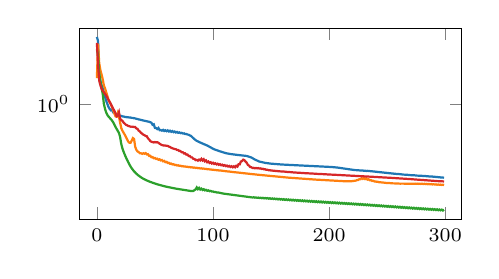
\begin{tikzpicture}

\definecolor{crimson2143940}{RGB}{214,39,40}
\definecolor{darkgray176}{RGB}{176,176,176}
\definecolor{darkorange25512714}{RGB}{255,127,14}
\definecolor{forestgreen4416044}{RGB}{44,160,44}
\definecolor{steelblue31119180}{RGB}{31,119,180}

\begin{axis}[compar,
	ymode=log]
\addplot [thick, steelblue31119180]
table {%
0 3.68010640144348
1 3.39949631690979
2 1.76648807525635
3 1.57563400268555
4 1.45096933841705
5 1.36281454563141
7 1.15613782405853
8 1.07007730007172
10 0.949615001678467
11 0.915130138397217
12 0.891516447067261
13 0.904359102249146
14 0.854554653167725
15 0.845201253890991
16 0.830264568328857
17 0.828166007995605
18 0.814599871635437
19 0.81267237663269
20 0.801861166954041
21 0.799715757369995
22 0.791904926300049
23 0.790146350860596
24 0.784241676330566
25 0.78319263458252
26 0.778436541557312
27 0.77826452255249
28 0.773918628692627
29 0.774324774742126
30 0.769253492355347
31 0.769412875175476
32 0.762951850891113
33 0.762222766876221
34 0.755105018615723
35 0.753398895263672
36 0.746738314628601
37 0.744306683540344
38 0.73854398727417
39 0.73573625087738
40 0.730782270431519
41 0.727953553199768
42 0.723552703857422
43 0.720949649810791
44 0.716549396514893
45 0.713973522186279
47 0.699978113174438
48 0.672848701477051
49 0.678932428359985
50 0.633800268173218
51 0.63248348236084
52 0.620214700698853
53 0.633156776428223
54 0.606647610664368
55 0.607864260673523
56 0.601230502128601
57 0.610259056091309
58 0.597402572631836
59 0.605943918228149
60 0.594431400299072
61 0.604331731796265
62 0.591032266616821
63 0.60042130947113
64 0.587352275848389
65 0.595834016799927
66 0.583614945411682
67 0.590960025787354
68 0.579948425292969
69 0.586132287979126
70 0.57629919052124
71 0.581279754638672
72 0.572519779205322
73 0.576217770576477
74 0.568392753601074
75 0.570689916610718
76 0.563570857048035
77 0.564261794090271
78 0.557365536689758
79 0.555926322937012
80 0.548094272613525
81 0.543044090270996
84 0.509581804275513
86 0.493227481842041
90 0.472973108291626
95 0.450887203216553
98 0.43472146987915
100 0.423869490623474
102 0.415469646453857
106 0.403010845184326
111 0.389142870903015
115 0.382572889328003
120 0.377117156982422
129 0.368658065795898
133 0.35810661315918
136 0.343956708908081
140 0.330448746681213
145 0.322344064712524
150 0.317590355873108
159 0.312477469444275
174 0.307183027267456
202 0.29775857925415
207 0.294676780700684
222 0.280587673187256
225 0.279558062553406
228 0.277686834335327
229 0.278058528900146
230 0.276828050613403
231 0.277303695678711
232 0.27591872215271
233 0.276457190513611
234 0.27492094039917
235 0.275482177734375
236 0.273820877075195
237 0.274370670318604
238 0.272625207901001
239 0.273138999938965
240 0.271354675292969
241 0.271817922592163
242 0.270036220550537
243 0.270443439483643
244 0.268697023391724
245 0.269048690795898
246 0.267360329627991
247 0.267661213874817
248 0.26604425907135
249 0.266301274299622
250 0.264761567115784
251 0.264982342720032
252 0.26352059841156
253 0.263713479042053
254 0.262325763702393
255 0.262498378753662
256 0.261179447174072
257 0.261338949203491
258 0.26008129119873
259 0.260234117507935
261 0.259182095527649
264 0.257060527801514
267 0.256314396858215
270 0.254393219947815
273 0.253796696662903
276 0.251975178718567
279 0.251482963562012
282 0.249649405479431
283 0.249951958656311
284 0.248858690261841
285 0.249161720275879
286 0.248045086860657
287 0.248341202735901
288 0.247198939323425
289 0.247479677200317
290 0.246309995651245
291 0.24656617641449
292 0.245367765426636
293 0.2455894947052
294 0.244361162185669
295 0.244538426399231
296 0.243278503417969
297 0.243400931358337
299 0.242164731025696
};
\addplot [thick, darkorange25512714]
table {%
0 1.65738987922668
1 3.2266047000885
2 2.20835661888123
3 1.93761301040649
4 1.78366184234619
5 1.62688362598419
6 1.43976211547852
7 1.36262428760529
9 1.17809808254242
10 1.09532189369202
11 1.04199075698853
12 0.997702598571777
13 0.950667142868042
14 0.89704430103302
15 0.840799808502197
16 0.792805194854736
17 0.789065003395081
18 0.846688270568848
19 0.784441471099854
21 0.630486845970154
22 0.60062313079834
23 0.577242612838745
24 0.555960416793823
26 0.507966995239258
27 0.486083507537842
28 0.475870370864868
29 0.475818037986755
30 0.496069669723511
31 0.520452499389648
32 0.512127161026001
33 0.439760446548462
34 0.414923071861267
35 0.401833891868591
36 0.397703766822815
37 0.388451099395752
38 0.388411164283752
39 0.383988261222839
40 0.38861095905304
41 0.384793400764465
42 0.389385104179382
43 0.379829049110413
44 0.381364345550537
45 0.368758201599121
46 0.36955738067627
47 0.359375834465027
48 0.360617399215698
49 0.352698445320129
50 0.354493379592896
51 0.347575902938843
52 0.349886894226074
53 0.342913269996643
54 0.345581293106079
55 0.337940096855164
56 0.340725064277649
57 0.332462787628174
58 0.335094094276428
59 0.326834678649902
60 0.329075813293457
61 0.321542859077454
62 0.323325872421265
63 0.316883325576782
64 0.318283319473267
65 0.312919974327087
66 0.314047336578369
67 0.309581637382507
68 0.310527086257935
69 0.306753039360046
70 0.307579755783081
71 0.304321885108948
72 0.305071353912354
73 0.302193164825439
74 0.302891135215759
75 0.300291299819946
76 0.300953030586243
77 0.298556566238403
78 0.299190640449524
79 0.296942830085754
80 0.297553300857544
81 0.295414209365845
82 0.296001195907593
83 0.293942928314209
84 0.294504523277283
85 0.292508006095886
86 0.293040871620178
87 0.291094064712524
88 0.291593790054321
89 0.289690375328064
90 0.290152430534363
91 0.288290143013
92 0.288709402084351
93 0.2868891954422
94 0.287260770797729
95 0.285485506057739
96 0.285804867744446
97 0.284079194068909
98 0.284342288970947
99 0.282671093940735
100 0.282874345779419
101 0.281262636184692
102 0.281403303146362
103 0.279855847358704
104 0.279932022094727
105 0.27845287322998
106 0.278463363647461
108 0.276999950408936
111 0.274283289909363
114 0.272668123245239
117 0.270202398300171
122 0.267102479934692
128 0.263124108314514
139 0.256230235099792
165 0.242330312728882
188 0.233508825302124
214 0.225921869277954
219 0.226001739501953
223 0.228850364685059
224 0.231322526931763
225 0.231699466705322
226 0.235517859458923
227 0.234749436378479
228 0.239452958106995
229 0.236430764198303
230 0.240861177444458
231 0.235719680786133
232 0.238932967185974
233 0.233223795890808
234 0.23513400554657
235 0.230209231376648
236 0.231216192245483
237 0.227456212043762
238 0.227952718734741
239 0.225188851356506
240 0.225422143936157
241 0.22337543964386
242 0.223478436470032
243 0.221918702125549
246 0.220745205879211
249 0.218888163566589
252 0.21820855140686
255 0.216981053352356
258 0.216687560081482
261 0.215785980224609
264 0.215937733650208
267 0.215198278427124
270 0.21584141254425
271 0.215040922164917
272 0.215885519981384
273 0.214976787567139
274 0.215919733047485
275 0.214887142181396
276 0.215909242630005
277 0.214746594429016
278 0.21582305431366
279 0.21453595161438
280 0.215640068054199
281 0.214246273040771
282 0.21535325050354
283 0.213879346847534
284 0.214969992637634
285 0.213447093963623
286 0.214509248733521
287 0.212966918945312
288 0.213995099067688
289 0.212458491325378
290 0.213453650474548
291 0.211940407752991
292 0.212907195091248
293 0.211427927017212
294 0.212373971939087
295 0.210932850837708
296 0.211866617202759
297 0.210462808609009
298 0.211392879486084
299 0.210021615028381
};
\addplot [thick, forestgreen4416044]
table {%
0 2.90652799606323
1 2.58646440505981
2 1.83608746528625
3 1.55235946178436
5 1.22411453723907
6 1.01032400131226
7 0.916084289550781
8 0.85399341583252
9 0.814010620117188
10 0.790211915969849
13 0.731614351272583
14 0.706826329231262
15 0.675795316696167
16 0.646470785140991
19 0.574944138526917
20 0.531929731369019
21 0.464287877082825
22 0.426081895828247
23 0.399688243865967
24 0.377828121185303
25 0.358893394470215
26 0.341920852661133
27 0.326518535614014
28 0.312665343284607
29 0.300542593002319
30 0.29019558429718
32 0.273862719535828
34 0.261515259742737
36 0.251717090606689
39 0.240297913551331
42 0.231782674789429
46 0.223130464553833
52 0.213074803352356
59 0.204237818717957
68 0.195970177650452
81 0.187185168266296
83 0.187378644943237
85 0.193094611167908
86 0.200681209564209
87 0.194102883338928
88 0.198964953422546
89 0.192695260047913
90 0.196166157722473
91 0.191070795059204
92 0.193764209747314
93 0.189497947692871
94 0.191552758216858
95 0.188003301620483
96 0.189515113830566
97 0.186544895172119
98 0.187583923339844
99 0.185100317001343
100 0.185735106468201
101 0.183662414550781
102 0.18395733833313
103 0.18223237991333
104 0.182247996330261
106 0.180607318878174
109 0.178060412406921
134 0.16520369052887
135 0.165813207626343
136 0.164600133895874
137 0.165334105491638
138 0.164031744003296
139 0.164887428283691
140 0.16348659992218
141 0.164458155632019
142 0.16295337677002
143 0.164032936096191
144 0.162422895431519
145 0.163601040840149
146 0.1618891954422
147 0.163157224655151
148 0.161349892616272
149 0.162700057029724
150 0.160805463790894
151 0.162231802940369
152 0.160258531570435
153 0.161756753921509
154 0.159712195396423
155 0.161279320716858
156 0.159169673919678
157 0.160802960395813
158 0.158632636070251
159 0.160329699516296
160 0.158102512359619
161 0.159860134124756
162 0.157579302787781
163 0.159394264221191
164 0.157062768936157
165 0.158930897712708
166 0.156552076339722
167 0.158468961715698
168 0.156046986579895
169 0.158008337020874
170 0.155547142028809
171 0.157548785209656
172 0.155052781105042
173 0.157090306282043
174 0.154564023017883
175 0.156633615493774
176 0.154081463813782
177 0.156178951263428
178 0.153605461120605
179 0.15572714805603
180 0.153136491775513
181 0.155278444290161
182 0.152674555778503
183 0.154833316802979
184 0.152220249176025
185 0.154392123222351
186 0.1517733335495
187 0.153954744338989
188 0.151333689689636
189 0.153521299362183
190 0.150901079177856
191 0.153091192245483
192 0.150475144386292
193 0.152664661407471
194 0.150055408477783
195 0.152240872383118
196 0.149641156196594
197 0.151819944381714
198 0.149232029914856
199 0.151401519775391
200 0.148827314376831
201 0.150984764099121
202 0.148425698280334
203 0.150569319725037
204 0.148026704788208
205 0.15015435218811
206 0.147629022598267
207 0.149739623069763
208 0.147231936454773
209 0.149324178695679
210 0.146834254264832
211 0.148907542228699
212 0.146435260772705
213 0.148489236831665
214 0.146034002304077
215 0.14806854724884
216 0.145629644393921
217 0.147645473480225
218 0.145221829414368
219 0.147219777107239
220 0.14480996131897
221 0.146790742874146
222 0.1443932056427
223 0.146358013153076
224 0.143972158432007
225 0.145922541618347
226 0.143546223640442
227 0.14548397064209
228 0.143115878105164
229 0.145042538642883
230 0.142681241035461
231 0.144598484039307
232 0.142242431640625
233 0.144151926040649
234 0.141799926757812
235 0.14370322227478
236 0.141354084014893
237 0.143253087997437
238 0.140905976295471
239 0.142802119255066
240 0.140455484390259
241 0.142350077629089
242 0.140003442764282
243 0.141897678375244
244 0.139550685882568
245 0.141445398330688
246 0.139097452163696
247 0.14099383354187
248 0.138644337654114
249 0.140542984008789
250 0.138192176818848
251 0.140093684196472
252 0.137741327285767
253 0.139646291732788
254 0.137292504310608
255 0.139200687408447
256 0.136845469474792
257 0.138757109642029
258 0.136401295661926
259 0.13831627368927
260 0.135960102081299
261 0.13787853717804
262 0.135522603988647
263 0.137443900108337
264 0.135088801383972
265 0.137012481689453
266 0.134658694267273
267 0.136584281921387
268 0.134233117103577
269 0.136159896850586
270 0.133811712265015
271 0.135739088058472
272 0.133395195007324
273 0.135322451591492
274 0.132983326911926
275 0.134909510612488
276 0.13257622718811
277 0.134500741958618
278 0.132174253463745
279 0.134095907211304
280 0.131777286529541
281 0.133695125579834
282 0.131385207176208
283 0.133298516273499
284 0.130998373031616
285 0.132905840873718
286 0.130616307258606
287 0.132517218589783
288 0.130239486694336
289 0.132132530212402
290 0.129867553710938
291 0.131751775741577
292 0.129500865936279
293 0.131375193595886
294 0.129138946533203
295 0.13100266456604
296 0.128782033920288
297 0.13063383102417
298 0.128429651260376
299 0.130268692970276
};
\addplot [thick, crimson2143940]
table {%
0 3.27433013916016
1 2.15141916275024
2 1.5779093503952
3 1.44807827472687
4 1.35112762451172
5 1.30105173587799
7 1.22471153736115
8 1.18338370323181
10 1.08618628978729
11 1.0482120513916
12 1.00823366641998
13 0.959881782531738
14 0.919629812240601
15 0.884634137153625
16 0.842983365058899
17 0.793495178222656
18 0.805639028549194
19 0.858284473419189
20 0.754631996154785
21 0.737125396728516
22 0.726847648620605
23 0.701433658599854
24 0.688852310180664
25 0.673883199691772
26 0.667015433311462
27 0.657734394073486
28 0.654704093933105
29 0.649169445037842
30 0.649649739265442
31 0.648463249206543
32 0.645026922225952
33 0.644170761108398
34 0.627417325973511
35 0.621903896331787
36 0.600471019744873
37 0.592319846153259
38 0.575231313705444
39 0.566770792007446
40 0.555399179458618
41 0.550884962081909
42 0.542288422584534
43 0.539475798606873
44 0.517281770706177
45 0.506843328475952
46 0.491036772727966
47 0.484905958175659
49 0.478334188461304
50 0.48267388343811
51 0.478787422180176
52 0.480922341346741
53 0.475183367729187
54 0.466984510421753
56 0.454699754714966
58 0.450355052947998
59 0.450329899787903
61 0.447613835334778
62 0.441530108451843
63 0.438369274139404
64 0.431590437889099
67 0.421071410179138
68 0.420159935951233
69 0.413992524147034
70 0.413689732551575
71 0.405237555503845
72 0.404957890510559
73 0.395872592926025
74 0.396290898323059
75 0.386945009231567
76 0.388152480125427
77 0.378128409385681
78 0.379216551780701
79 0.368839621543884
80 0.369049072265625
81 0.358893156051636
82 0.358290791511536
83 0.348625659942627
84 0.348151087760925
85 0.340011477470398
86 0.341872692108154
87 0.336538076400757
88 0.343466281890869
89 0.338452816009521
90 0.34873902797699
91 0.337954044342041
92 0.346057653427124
93 0.332503080368042
94 0.338034510612488
95 0.326400876045227
96 0.331196188926697
97 0.321815013885498
98 0.326478958129883
99 0.318461418151855
100 0.323017954826355
101 0.31570029258728
102 0.320061445236206
103 0.313133001327515
104 0.317217230796814
105 0.310580253601074
106 0.314353585243225
107 0.307995080947876
108 0.311489582061768
109 0.305393099784851
110 0.308713436126709
111 0.302810668945312
112 0.306141495704651
113 0.30030345916748
114 0.303930163383484
115 0.298001289367676
116 0.302364826202393
117 0.296278357505798
118 0.302110910415649
119 0.296181201934814
120 0.304772138595581
121 0.30031681060791
122 0.313632488250732
123 0.313233256340027
124 0.330968856811523
125 0.333672523498535
126 0.343123078346252
127 0.340104937553406
128 0.330533146858215
129 0.323531150817871
130 0.310237407684326
131 0.305840492248535
132 0.297647833824158
133 0.296418786048889
134 0.292115449905396
135 0.292920708656311
136 0.290423393249512
137 0.292078375816345
138 0.289920568466187
139 0.291498064994812
140 0.288926482200623
141 0.289979696273804
142 0.286918878555298
143 0.287495970726013
144 0.284289836883545
145 0.284648537635803
146 0.281665921211243
147 0.282004356384277
148 0.279434442520142
149 0.279824256896973
150 0.277694463729858
151 0.278121471405029
152 0.276376962661743
153 0.276788711547852
154 0.275345206260681
155 0.275684475898743
156 0.274452090263367
158 0.273577570915222
161 0.272650718688965
164 0.270642518997192
167 0.26951014995575
170 0.267747521400452
175 0.266040444374084
180 0.263978600502014
185 0.262534737586975
190 0.260632991790771
195 0.259276986122131
200 0.257510662078857
207 0.255552530288696
216 0.252692699432373
238 0.24614417552948
247 0.243234276771545
254 0.241256356239319
261 0.238715171813965
268 0.236382484436035
277 0.2327481508255
286 0.229421734809875
293 0.22672963142395
298 0.225495457649231
299 0.224904894828796
};
\end{axis}

\end{tikzpicture}
}
	&
	\multicolumn{4}{c}{% This file was created with tikzplotlib v0.10.1.
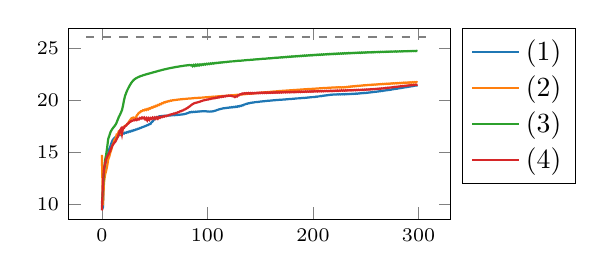
\begin{tikzpicture}

\definecolor{crimson2143940}{RGB}{214,39,40}
\definecolor{darkgray176}{RGB}{176,176,176}
\definecolor{darkorange25512714}{RGB}{255,127,14}
\definecolor{forestgreen4416044}{RGB}{44,160,44}
\definecolor{steelblue31119180}{RGB}{31,119,180}

\begin{axis}[compar, legend pos=outer north east]
\addplot [thick, steelblue31119180]
table {%
0 9.52000045776367
1 9.73999977111816
2 13.2399997711182
3 13.7299995422363
4 14.1000003814697
5 14.460000038147
6 14.8699998855591
7 15.3100004196167
8 15.5699996948242
9 15.8800001144409
10 16.1299991607666
11 16.2800006866455
12 16.3899993896484
13 16.2700004577637
14 16.5300006866455
15 16.5499992370605
16 16.6599998474121
17 16.6399993896484
18 16.75
19 16.7299995422363
20 16.8199996948242
21 16.7999992370605
22 16.8899993896484
23 16.8700008392334
24 16.9500007629395
25 16.9300003051758
26 17.0100002288818
27 16.9899997711182
28 17.0699996948242
29 17.0499992370605
30 17.1299991607666
31 17.1200008392334
32 17.1900005340576
33 17.1900005340576
34 17.2600002288818
35 17.2700004577637
36 17.3299999237061
37 17.3500003814697
38 17.3999996185303
39 17.4400005340576
40 17.4699993133545
41 17.5200004577637
42 17.5499992370605
43 17.6100006103516
44 17.6200008392334
45 17.7099990844727
46 17.7099990844727
47 17.8799991607666
48 17.9500007629395
49 18.0900001525879
50 18.25
51 18.3299999237061
52 18.3400001525879
53 18.3799991607666
54 18.4400005340576
55 18.4699993133545
56 18.4699993133545
60 18.5100002288818
61 18.5
62 18.5200004577637
63 18.5200004577637
64 18.5400009155273
65 18.5300006866455
66 18.5499992370605
67 18.5499992370605
68 18.5699996948242
69 18.5599994659424
70 18.5799999237061
71 18.5799999237061
76 18.6299991607666
77 18.6499996185303
78 18.6599998474121
79 18.6900005340576
80 18.7099990844727
81 18.7600002288818
82 18.7800006866455
83 18.8400001525879
84 18.8299999237061
85 18.8799991607666
86 18.8500003814697
87 18.8899993896484
88 18.8600006103516
89 18.8999996185303
90 18.8799991607666
91 18.9200000762939
92 18.8999996185303
93 18.9300003051758
94 18.9200000762939
95 18.9400005340576
96 18.9300003051758
97 18.9400005340576
98 18.9300003051758
99 18.9300003051758
100 18.9099998474121
101 18.9099998474121
102 18.8999996185303
103 18.9099998474121
104 18.9099998474121
106 18.9500007629395
108 19.0100002288818
109 19.0499992370605
110 19.0799999237061
111 19.1200008392334
112 19.1399993896484
113 19.1700000762939
114 19.1900005340576
115 19.2199993133545
116 19.2199993133545
117 19.25
118 19.25
119 19.2800006866455
120 19.2700004577637
121 19.3099994659424
122 19.2900009155273
123 19.3400001525879
124 19.3099994659424
125 19.3600006103516
126 19.3299999237061
127 19.3899993896484
128 19.3500003814697
129 19.4200000762939
130 19.3899993896484
131 19.4599990844727
132 19.4400005340576
133 19.5100002288818
134 19.5100002288818
135 19.5900001525879
136 19.6000003814697
137 19.6599998474121
138 19.6599998474121
139 19.7099990844727
140 19.7099990844727
141 19.75
142 19.75
143 19.7800006866455
144 19.7800006866455
145 19.8099994659424
146 19.8099994659424
147 19.8299999237061
148 19.8299999237061
149 19.8500003814697
150 19.8600006103516
151 19.8799991607666
152 19.8799991607666
153 19.8999996185303
154 19.8999996185303
155 19.9200000762939
156 19.9200000762939
157 19.9400005340576
158 19.9400005340576
163 19.9899997711182
164 19.9899997711182
165 20.0100002288818
166 20.0100002288818
169 20.0400009155273
170 20.0400009155273
173 20.0699996948242
174 20.0699996948242
175 20.0900001525879
176 20.0900001525879
177 20.1000003814697
178 20.1000003814697
179 20.1200008392334
180 20.1200008392334
181 20.1299991607666
182 20.1299991607666
183 20.1499996185303
184 20.1499996185303
185 20.1700000762939
186 20.1700000762939
187 20.1800003051758
188 20.1800003051758
189 20.2000007629395
190 20.2000007629395
191 20.2199993133545
192 20.2099990844727
193 20.2299995422363
194 20.2299995422363
195 20.25
196 20.25
197 20.2700004577637
198 20.2700004577637
199 20.2900009155273
200 20.2900009155273
201 20.3099994659424
202 20.3099994659424
203 20.3400001525879
204 20.3299999237061
205 20.3600006103516
206 20.3600006103516
207 20.3899993896484
208 20.3799991607666
209 20.4200000762939
210 20.4099998474121
211 20.4500007629395
212 20.4400005340576
213 20.4799995422363
214 20.4699993133545
215 20.5
216 20.5
217 20.5300006866455
218 20.5100002288818
219 20.5400009155273
220 20.5300006866455
221 20.5499992370605
222 20.5400009155273
223 20.5599994659424
224 20.5400009155273
225 20.5699996948242
226 20.5400009155273
227 20.5699996948242
228 20.5499992370605
229 20.5799999237061
230 20.5499992370605
231 20.5900001525879
232 20.5599994659424
233 20.5900001525879
234 20.5699996948242
235 20.6000003814697
236 20.5799999237061
237 20.6100006103516
238 20.5900001525879
239 20.6200008392334
240 20.6000003814697
241 20.6399993896484
242 20.6100006103516
243 20.6499996185303
244 20.6299991607666
245 20.6700000762939
246 20.6499996185303
247 20.6800003051758
248 20.6700000762939
249 20.7000007629395
250 20.6800003051758
251 20.7199993133545
252 20.7099990844727
253 20.7399997711182
254 20.7299995422363
255 20.7600002288818
256 20.75
257 20.7900009155273
258 20.7800006866455
259 20.8099994659424
260 20.7999992370605
261 20.8299999237061
262 20.8299999237061
263 20.8600006103516
264 20.8600006103516
265 20.8899993896484
266 20.8799991607666
267 20.9200000762939
268 20.9099998474121
269 20.9500007629395
270 20.9400005340576
271 20.9699993133545
272 20.9699993133545
273 21.0100002288818
274 21
275 21.0400009155273
276 21.0400009155273
277 21.0699996948242
278 21.0699996948242
279 21.1000003814697
280 21.1000003814697
281 21.1299991607666
282 21.1299991607666
283 21.1599998474121
284 21.1700000762939
285 21.1900005340576
286 21.2000007629395
287 21.2299995422363
288 21.2299995422363
289 21.2600002288818
290 21.2600002288818
291 21.2900009155273
292 21.2999992370605
293 21.3299999237061
294 21.3299999237061
295 21.3600006103516
296 21.3700008392334
297 21.3999996185303
298 21.3999996185303
299 21.4300003051758
};
\addlegendentry{$(1)$}
\addplot [thick, darkorange25512714]
table {%
0 14.7600002288818
1 9.9399995803833
2 12.1099996566772
3 12.8500003814697
4 13.2200002670288
5 13.6899995803833
6 14.3299999237061
7 14.5900001525879
8 14.9799995422363
9 15.2799997329712
10 15.6899995803833
11 15.8999996185303
12 16.2199993133545
13 16.3299999237061
14 16.7099990844727
15 16.7099990844727
16 17.0200004577637
17 17.0799999237061
18 16.8099994659424
19 16.9300003051758
20 17.3299999237061
21 17.4599990844727
22 17.5499992370605
23 17.6000003814697
24 17.7099990844727
25 17.8299999237061
26 17.9899997711182
27 18.1299991607666
28 18.2600002288818
29 18.3099994659424
30 18.3400001525879
31 18.2900009155273
32 18.25
33 18.5200004577637
34 18.6399993896484
35 18.7800006866455
36 18.8299999237061
37 18.9400005340576
38 18.9500007629395
39 19.0400009155273
40 19.0100002288818
41 19.1000003814697
42 19.0499992370605
43 19.1599998474121
44 19.1100006103516
45 19.2299995422363
46 19.2000007629395
47 19.3099994659424
48 19.2800006866455
49 19.3799991607666
50 19.3600006103516
51 19.4599990844727
52 19.4300003051758
53 19.5400009155273
54 19.5200004577637
55 19.6299991607666
56 19.6100006103516
57 19.7199993133545
58 19.7000007629395
59 19.7999992370605
60 19.7800006866455
61 19.8600006103516
62 19.8500003814697
63 19.9099998474121
64 19.8999996185303
65 19.9599990844727
66 19.9500007629395
67 19.9899997711182
68 19.9899997711182
69 20.0200004577637
70 20.0200004577637
71 20.0400009155273
72 20.0499992370605
73 20.0699996948242
74 20.0699996948242
75 20.0900001525879
76 20.0900001525879
77 20.1100006103516
78 20.1100006103516
83 20.1599998474121
84 20.1599998474121
88 20.2000007629395
89 20.2000007629395
92 20.2299995422363
93 20.2299995422363
94 20.2399997711182
95 20.2399997711182
96 20.2600002288818
97 20.2600002288818
98 20.2700004577637
99 20.2700004577637
100 20.2900009155273
101 20.2900009155273
102 20.3099994659424
103 20.2999992370605
104 20.3199996948242
105 20.3199996948242
106 20.3400001525879
107 20.3299999237061
108 20.3500003814697
109 20.3500003814697
110 20.3700008392334
111 20.3600006103516
112 20.3799991607666
113 20.3799991607666
114 20.3999996185303
115 20.3899993896484
116 20.4099998474121
117 20.4099998474121
118 20.4300003051758
119 20.4300003051758
120 20.4400005340576
121 20.4400005340576
122 20.4599990844727
123 20.4599990844727
124 20.4799995422363
125 20.4699993133545
126 20.4899997711182
127 20.4899997711182
128 20.5100002288818
129 20.5100002288818
130 20.5300006866455
131 20.5300006866455
132 20.5400009155273
133 20.5400009155273
134 20.5599994659424
135 20.5599994659424
136 20.5799999237061
137 20.5799999237061
138 20.6000003814697
139 20.6000003814697
148 20.6900005340576
149 20.6900005340576
150 20.7099990844727
151 20.7099990844727
152 20.7299995422363
153 20.7299995422363
154 20.75
155 20.75
162 20.8199996948242
163 20.8199996948242
168 20.8700008392334
169 20.8700008392334
172 20.8999996185303
173 20.8999996185303
176 20.9300003051758
177 20.9300003051758
180 20.9599990844727
181 20.9599990844727
183 20.9799995422363
184 20.9799995422363
186 21
187 21
190 21.0300006866455
191 21.0300006866455
192 21.0400009155273
193 21.0400009155273
196 21.0699996948242
197 21.0699996948242
198 21.0799999237061
199 21.0799999237061
201 21.1000003814697
202 21.1000003814697
204 21.1200008392334
205 21.1200008392334
206 21.1299991607666
207 21.1299991607666
210 21.1599998474121
211 21.1599998474121
212 21.1700000762939
213 21.1700000762939
214 21.1800003051758
215 21.1800003051758
216 21.2000007629395
217 21.1900005340576
218 21.2099990844727
219 21.2000007629395
220 21.2199993133545
221 21.2000007629395
222 21.2299995422363
223 21.2099990844727
224 21.2399997711182
225 21.2099990844727
226 21.2399997711182
227 21.2000007629395
228 21.2399997711182
229 21.2099990844727
230 21.25
231 21.2199993133545
232 21.2700004577637
233 21.2399997711182
234 21.2999992370605
235 21.2600002288818
236 21.3199996948242
237 21.2900009155273
238 21.3400001525879
239 21.3099994659424
240 21.3600006103516
241 21.3299999237061
242 21.3799991607666
243 21.3500003814697
244 21.3899993896484
245 21.3700008392334
246 21.4099998474121
247 21.3899993896484
248 21.4300003051758
249 21.4099998474121
250 21.4400005340576
251 21.4200000762939
252 21.4599990844727
253 21.4400005340576
254 21.4699993133545
255 21.4500007629395
256 21.4899997711182
257 21.4699993133545
258 21.5
259 21.4799995422363
260 21.5100002288818
261 21.4899997711182
262 21.5300006866455
263 21.5100002288818
264 21.5400009155273
265 21.5200004577637
266 21.5599994659424
267 21.5300006866455
268 21.5699996948242
269 21.5400009155273
270 21.5799999237061
271 21.5499992370605
272 21.5900001525879
273 21.5599994659424
274 21.6100006103516
275 21.5799999237061
276 21.6200008392334
277 21.5900001525879
278 21.6299991607666
279 21.6000003814697
280 21.6399993896484
281 21.6100006103516
282 21.6499996185303
283 21.6200008392334
284 21.6599998474121
285 21.6299991607666
286 21.6800003051758
287 21.6399993896484
288 21.6900005340576
289 21.6499996185303
290 21.7000007629395
291 21.6599998474121
292 21.7099990844727
293 21.6700000762939
294 21.7199993133545
295 21.6800003051758
296 21.7299995422363
297 21.6900005340576
298 21.7399997711182
299 21.7000007629395
};
\addlegendentry{$(2)$}
\addplot [thick, forestgreen4416044]
table {%
0 10.0500001907349
1 11.5100002288818
2 13.2299995422363
3 14.2399997711182
4 14.7399997711182
5 15.4700002670288
6 16.2900009155273
7 16.5699996948242
8 16.8999996185303
9 17.1000003814697
10 17.2600002288818
12 17.5200004577637
13 17.6599998474121
14 17.8600006103516
15 18.1200008392334
16 18.3700008392334
17 18.5699996948242
19 19.0300006866455
20 19.4599990844727
21 20.0100002288818
22 20.4200000762939
23 20.6900005340576
24 20.9400005340576
26 21.3400001525879
27 21.5100002288818
28 21.6700000762939
29 21.7999992370605
30 21.9099998474121
31 22
32 22.0699996948242
33 22.1299991607666
35 22.2299995422363
37 22.3099994659424
38 22.3400001525879
39 22.3799991607666
44 22.5300006866455
45 22.5499992370605
49 22.6700000762939
50 22.6900005340576
54 22.8099994659424
55 22.8299999237061
57 22.8899993896484
58 22.9099998474121
59 22.9400005340576
61 22.9799995422363
62 23.0100002288818
71 23.1900005340576
72 23.2000007629395
74 23.2399997711182
75 23.25
76 23.2700004577637
77 23.2800006866455
78 23.2999992370605
80 23.3199996948242
81 23.3400001525879
82 23.3400001525879
83 23.3700008392334
84 23.3299999237061
85 23.3600006103516
86 23.25
87 23.3700008392334
88 23.2700004577637
89 23.3899993896484
90 23.2999992370605
91 23.4099998474121
92 23.3199996948242
93 23.4200000762939
94 23.3500003814697
95 23.4400005340576
96 23.3799991607666
97 23.4599990844727
98 23.3999996185303
99 23.4799995422363
100 23.4300003051758
101 23.5
102 23.4500007629395
103 23.5200004577637
104 23.4799995422363
105 23.5400009155273
106 23.5
107 23.5599994659424
108 23.5300006866455
109 23.5799999237061
110 23.5499992370605
111 23.6000003814697
112 23.5799999237061
113 23.6200008392334
114 23.6000003814697
115 23.6399993896484
116 23.6200008392334
117 23.6599998474121
118 23.6399993896484
119 23.6800003051758
120 23.6700000762939
121 23.6900005340576
122 23.6900005340576
123 23.7099990844727
124 23.7099990844727
125 23.7299995422363
126 23.7299995422363
127 23.75
128 23.75
129 23.7700004577637
130 23.7700004577637
131 23.7800006866455
132 23.7800006866455
133 23.7999992370605
134 23.7999992370605
138 23.8400001525879
139 23.8400001525879
142 23.8700008392334
143 23.8700008392334
144 23.8899993896484
145 23.8899993896484
146 23.9099998474121
147 23.8999996185303
148 23.9200000762939
149 23.9200000762939
150 23.9400005340576
151 23.9300003051758
152 23.9599990844727
153 23.9500007629395
154 23.9699993133545
155 23.9599990844727
156 23.9899997711182
157 23.9799995422363
158 24.0100002288818
159 23.9899997711182
160 24.0200004577637
161 24.0100002288818
162 24.0400009155273
163 24.0300006866455
164 24.0599994659424
165 24.0400009155273
166 24.0699996948242
167 24.0599994659424
168 24.0900001525879
169 24.0699996948242
170 24.1100006103516
171 24.0799999237061
172 24.1200008392334
173 24.1000003814697
174 24.1399993896484
175 24.1100006103516
176 24.1599998474121
177 24.1299991607666
178 24.1700000762939
179 24.1399993896484
180 24.1900005340576
181 24.1599998474121
182 24.2000007629395
183 24.1700000762939
184 24.2199993133545
185 24.1900005340576
186 24.2299995422363
187 24.2000007629395
188 24.25
189 24.2099990844727
190 24.2600002288818
191 24.2299995422363
192 24.2800006866455
193 24.2399997711182
194 24.2900009155273
195 24.2600002288818
196 24.2999992370605
197 24.2700004577637
198 24.3199996948242
199 24.2800006866455
200 24.3299999237061
201 24.2999992370605
202 24.3400001525879
203 24.3099994659424
204 24.3600006103516
205 24.3199996948242
206 24.3700008392334
207 24.3299999237061
208 24.3799991607666
209 24.3400001525879
210 24.3899993896484
211 24.3600006103516
212 24.3999996185303
213 24.3700008392334
214 24.4200000762939
215 24.3799991607666
216 24.4300003051758
217 24.3899993896484
218 24.4400005340576
219 24.3999996185303
220 24.4500007629395
221 24.4099998474121
222 24.4599990844727
223 24.4200000762939
224 24.4699993133545
225 24.4300003051758
226 24.4799995422363
227 24.4400005340576
228 24.4899997711182
229 24.4500007629395
230 24.5
231 24.4599990844727
232 24.5100002288818
233 24.4699993133545
234 24.5200004577637
235 24.4799995422363
236 24.5200004577637
237 24.4899997711182
238 24.5300006866455
239 24.5
240 24.5400009155273
241 24.5100002288818
242 24.5499992370605
243 24.5200004577637
244 24.5599994659424
245 24.5200004577637
246 24.5699996948242
247 24.5300006866455
248 24.5699996948242
249 24.5400009155273
250 24.5799999237061
251 24.5499992370605
252 24.5900001525879
253 24.5599994659424
254 24.5900001525879
255 24.5599994659424
256 24.6000003814697
257 24.5699996948242
258 24.6100006103516
259 24.5799999237061
260 24.6100006103516
261 24.5900001525879
262 24.6200008392334
263 24.5900001525879
264 24.6299991607666
265 24.6000003814697
266 24.6299991607666
267 24.6100006103516
268 24.6399993896484
269 24.6100006103516
270 24.6499996185303
271 24.6200008392334
272 24.6499996185303
273 24.6299991607666
274 24.6599998474121
275 24.6299991607666
276 24.6599998474121
277 24.6399993896484
278 24.6700000762939
279 24.6399993896484
280 24.6700000762939
281 24.6499996185303
282 24.6800003051758
283 24.6499996185303
284 24.6800003051758
285 24.6599998474121
286 24.6900005340576
287 24.6700000762939
288 24.6900005340576
289 24.6700000762939
290 24.7000007629395
291 24.6800003051758
292 24.7000007629395
293 24.6800003051758
294 24.7099990844727
295 24.6900005340576
296 24.7099990844727
297 24.6900005340576
298 24.7199993133545
299 24.7000007629395
};
\addlegendentry{$(3)$}
\addplot [thick, crimson2143940]
table {%
0 9.4399995803833
1 12.0500001907349
2 13.4899997711182
3 13.9300003051758
4 14.3400001525879
5 14.5799999237061
6 14.7600002288818
7 14.960000038147
8 15.1700000762939
9 15.4300003051758
10 15.6499996185303
11 15.8100004196167
12 15.9399995803833
13 16.0599994659424
14 16.2800006866455
15 16.4599990844727
16 16.7600002288818
17 17.0699996948242
18 17.2399997711182
19 16.75
20 17.3700008392334
21 17.3500003814697
22 17.5100002288818
23 17.5599994659424
24 17.7099990844727
25 17.7600002288818
26 17.8799991607666
27 17.9200000762939
28 18.0200004577637
29 18.0300006866455
30 18.1100006103516
31 18.0699996948242
32 18.1499996185303
33 18.0900001525879
34 18.2099990844727
35 18.1499996185303
36 18.2900009155273
37 18.2399997711182
38 18.3500003814697
39 18.2600002288818
40 18.3400001525879
41 18.1700000762939
42 18.2800006866455
43 18.0699996948242
44 18.2700004577637
45 18.1200008392334
46 18.2900009155273
47 18.2000007629395
48 18.3299999237061
49 18.2199993133545
50 18.3400001525879
51 18.2099990844727
52 18.3500003814697
53 18.2199993133545
54 18.3700008392334
55 18.2999992370605
56 18.4099998474121
57 18.3700008392334
58 18.4599990844727
59 18.4200000762939
60 18.4899997711182
61 18.4599990844727
62 18.5400009155273
63 18.5300006866455
64 18.6000003814697
65 18.6100006103516
66 18.6599998474121
67 18.6599998474121
68 18.7199993133545
69 18.7099990844727
70 18.7800006866455
71 18.7700004577637
72 18.8500003814697
73 18.8500003814697
74 18.9300003051758
75 18.9300003051758
76 19.0100002288818
77 19.0200004577637
78 19.1000003814697
79 19.1200008392334
80 19.2000007629395
81 19.2399997711182
82 19.3299999237061
83 19.3899993896484
84 19.4799995422363
86 19.6200008392334
87 19.6800003051758
88 19.7199993133545
89 19.75
90 19.7700004577637
93 19.8600006103516
94 19.8999996185303
95 19.9300003051758
96 19.9699993133545
97 19.9899997711182
98 20.0200004577637
99 20.0300006866455
100 20.0699996948242
101 20.0699996948242
102 20.1200008392334
103 20.1100006103516
104 20.1599998474121
105 20.1499996185303
106 20.2000007629395
107 20.1800003051758
108 20.2399997711182
109 20.2199993133545
110 20.2800006866455
111 20.25
112 20.3199996948242
113 20.2900009155273
114 20.3600006103516
115 20.3199996948242
116 20.3899993896484
117 20.3500003814697
118 20.4200000762939
119 20.3899993896484
120 20.4400005340576
121 20.4099998474121
122 20.4200000762939
123 20.3999996185303
124 20.3600006103516
125 20.3600006103516
126 20.2900009155273
127 20.3600006103516
128 20.3400001525879
129 20.4599990844727
130 20.4599990844727
131 20.5699996948242
132 20.5599994659424
133 20.6399993896484
134 20.6100006103516
135 20.6700000762939
136 20.6299991607666
137 20.6800003051758
138 20.6299991607666
139 20.6900005340576
140 20.6299991607666
141 20.6900005340576
142 20.6299991607666
143 20.6900005340576
144 20.6399993896484
145 20.7000007629395
146 20.6499996185303
147 20.7099990844727
148 20.6599998474121
149 20.7199993133545
150 20.6700000762939
151 20.7299995422363
152 20.6700000762939
153 20.7299995422363
154 20.6800003051758
155 20.7399997711182
156 20.6800003051758
157 20.7399997711182
158 20.6900005340576
159 20.7399997711182
160 20.6900005340576
161 20.75
162 20.7000007629395
163 20.75
164 20.7000007629395
165 20.7600002288818
166 20.7099990844727
167 20.7600002288818
168 20.7099990844727
169 20.7700004577637
170 20.7199993133545
171 20.7700004577637
172 20.7299995422363
173 20.7800006866455
174 20.7299995422363
175 20.7900009155273
176 20.7399997711182
177 20.7900009155273
178 20.7399997711182
179 20.7999992370605
180 20.75
181 20.7999992370605
182 20.75
183 20.8099994659424
184 20.7600002288818
185 20.8099994659424
186 20.7700004577637
187 20.8199996948242
188 20.7700004577637
189 20.8299999237061
190 20.7800006866455
191 20.8299999237061
192 20.7900009155273
193 20.8400001525879
194 20.7900009155273
195 20.8400001525879
196 20.7999992370605
197 20.8500003814697
198 20.7999992370605
199 20.8600006103516
200 20.8099994659424
201 20.8600006103516
202 20.8199996948242
203 20.8700008392334
204 20.8199996948242
205 20.8700008392334
206 20.8299999237061
207 20.8799991607666
208 20.8299999237061
209 20.8799991607666
210 20.8400001525879
211 20.8899993896484
212 20.8500003814697
213 20.8999996185303
214 20.8500003814697
215 20.8999996185303
216 20.8600006103516
217 20.9099998474121
218 20.8600006103516
219 20.9099998474121
220 20.8700008392334
221 20.9200000762939
222 20.8799991607666
223 20.9300003051758
224 20.8799991607666
225 20.9300003051758
226 20.8899993896484
227 20.9400005340576
228 20.8999996185303
229 20.9400005340576
230 20.8999996185303
231 20.9500007629395
232 20.9099998474121
233 20.9599990844727
234 20.9200000762939
235 20.9599990844727
236 20.9200000762939
237 20.9699993133545
238 20.9300003051758
239 20.9799995422363
240 20.9400005340576
241 20.9899997711182
242 20.9500007629395
243 21
244 20.9599990844727
245 21
246 20.9699993133545
247 21.0100002288818
248 20.9799995422363
249 21.0200004577637
250 20.9899997711182
251 21.0300006866455
252 21
253 21.0400009155273
254 21.0100002288818
255 21.0599994659424
256 21.0300006866455
257 21.0699996948242
258 21.0400009155273
259 21.0799999237061
260 21.0599994659424
261 21.1000003814697
262 21.0699996948242
263 21.1200008392334
264 21.0900001525879
265 21.1299991607666
266 21.1100006103516
267 21.1499996185303
268 21.1299991607666
269 21.1800003051758
270 21.1499996185303
271 21.2000007629395
272 21.1800003051758
273 21.2199993133545
274 21.2000007629395
275 21.2399997711182
276 21.2299995422363
277 21.2700004577637
278 21.25
279 21.2900009155273
280 21.2700004577637
281 21.3099994659424
282 21.2999992370605
283 21.3400001525879
284 21.3199996948242
285 21.3600006103516
286 21.3400001525879
287 21.3799991607666
288 21.3600006103516
289 21.3999996185303
290 21.3899993896484
291 21.4200000762939
292 21.4099998474121
293 21.4400005340576
294 21.4200000762939
295 21.4599990844727
296 21.4400005340576
297 21.4799995422363
298 21.4599990844727
299 21.5
};
\addlegendentry{$(4)$}
\addplot [thick, gray, dashed]
table {%
-14.95 26.0524063110352
313.95 26.0524063110352
};
\end{axis}

\end{tikzpicture}
}
\end{tabular}
	\caption{$d=200$, avec passe-base gaussien ($\sigma=0.6$)}
	\label{fig:LGDlat200-g}
\end{figure}

\begin{figure}[H]\centering
	\begin{tabular}{c c c c c c}
	Target  &  $(1)$  &  $(2)$  &  $(3)$   &  $(4)$
	
	\\
	
	\multirow{2}{0.3\textwidth}[0.122\textwidth]{\includegraphics[width=0.3\textwidth]{resultats/LGD/lats/lat-400-target-s.png}}
	&
	\includegraphics[width=0.15\textwidth]{resultats/LGD/lats/lat-400_1-init-pas=0.5_filtre=s-None.png}
	&
	\includegraphics[width=0.15\textwidth]{resultats/LGD/lats/lat-400_2-init-pas=0.5_filtre=s-None.png}
	&
	\includegraphics[width=0.15\textwidth]{resultats/LGD/lats/lat-400_3-init-pas=0.5_filtre=s-None.png}
	&
	\includegraphics[width=0.15\textwidth]{resultats/LGD/lats/lat-400_4-init-pas=0.5_filtre=s-None.png}
	
	\\
	
	
	&
	\includegraphics[width=0.15\textwidth]{resultats/LGD/lats/lat-400_1-guess-pas=0.5_filtre=s-None.png}
	&
	\includegraphics[width=0.15\textwidth]{resultats/LGD/lats/lat-400_2-guess-pas=0.5_filtre=s-None.png}
	&
	\includegraphics[width=0.15\textwidth]{resultats/LGD/lats/lat-400_3-guess-pas=0.5_filtre=s-None.png}
	&
	\includegraphics[width=0.15\textwidth]{resultats/LGD/lats/lat-400_4-guess-pas=0.5_filtre=s-None.png}
	
	\\ \\
	
	
	
	\multicolumn{2}{c}{Loss}  &  \multicolumn{4}{c}{PSNR{\color{white}bbbb}}
	
	\\
	
	\multicolumn{2}{c}{% This file was created with tikzplotlib v0.10.1.
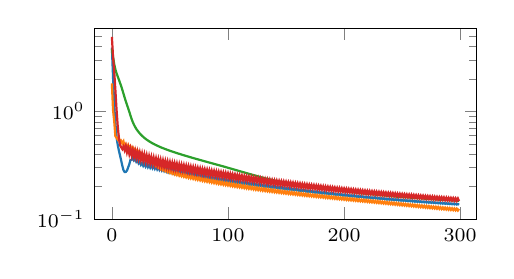
\begin{tikzpicture}

\definecolor{crimson2143940}{RGB}{214,39,40}
\definecolor{darkgray176}{RGB}{176,176,176}
\definecolor{darkorange25512714}{RGB}{255,127,14}
\definecolor{forestgreen4416044}{RGB}{44,160,44}
\definecolor{steelblue31119180}{RGB}{31,119,180}

\begin{axis}[compar,
	ymode=log]
\addplot [thick, steelblue31119180]
table {%
0 3.91733932495117
1 2.06791567802429
2 1.12501072883606
3 0.783846616744995
4 0.57644510269165
5 0.49086320400238
6 0.4333336353302
7 0.390443921089172
9 0.312576055526733
10 0.284053683280945
11 0.273382782936096
12 0.274090766906738
13 0.281869649887085
14 0.30110490322113
15 0.322925925254822
16 0.354105234146118
17 0.355159997940063
18 0.372391581535339
19 0.351119160652161
20 0.362392544746399
21 0.340497374534607
22 0.351433515548706
23 0.329342842102051
24 0.341014862060547
25 0.31944751739502
26 0.332684278488159
27 0.312301516532898
28 0.327115535736084
29 0.307612299919128
30 0.323195815086365
31 0.303920388221741
32 0.319617390632629
33 0.300405979156494
34 0.315970778465271
35 0.296917200088501
36 0.312297821044922
37 0.293479800224304
38 0.308663129806519
39 0.290117859840393
40 0.305089473724365
41 0.286843776702881
42 0.301589250564575
43 0.283659815788269
44 0.298163890838623
45 0.280564546585083
46 0.294817686080933
47 0.277557134628296
48 0.291549563407898
49 0.274632811546326
50 0.288360714912415
51 0.271790862083435
52 0.285251021385193
53 0.269027709960938
54 0.2822185754776
55 0.266339540481567
56 0.27926242351532
57 0.263725161552429
58 0.276380896568298
59 0.261180877685547
60 0.273573160171509
61 0.258704900741577
62 0.270836710929871
63 0.256294727325439
64 0.268169760704041
65 0.253947019577026
66 0.265570044517517
67 0.251660346984863
68 0.263035297393799
69 0.249431371688843
70 0.260563850402832
71 0.247259378433228
72 0.258153915405273
73 0.245140314102173
74 0.255802273750305
75 0.243073582649231
76 0.253507614135742
77 0.241056323051453
78 0.25126838684082
79 0.239087700843811
80 0.249082684516907
81 0.23716402053833
82 0.246946811676025
83 0.235284566879272
84 0.244860053062439
85 0.233446478843689
86 0.242820262908936
87 0.231649160385132
88 0.240825891494751
89 0.229890823364258
90 0.2388756275177
91 0.228170037269592
92 0.236967444419861
93 0.226484775543213
94 0.235099077224731
95 0.224833011627197
96 0.233268857002258
97 0.223214626312256
98 0.231476545333862
99 0.221626996994019
100 0.229718446731567
101 0.220068335533142
102 0.227995038032532
103 0.218539476394653
104 0.226304769515991
105 0.217038154602051
106 0.224646091461182
107 0.215563416481018
108 0.223017811775208
109 0.214113473892212
110 0.221418380737305
111 0.212688684463501
112 0.219847679138184
113 0.211286067962646
114 0.218302965164185
115 0.209906816482544
116 0.216785192489624
117 0.208549499511719
118 0.21529221534729
119 0.207211971282959
120 0.213822841644287
121 0.205893635749817
122 0.21237576007843
123 0.204594731330872
124 0.210951447486877
125 0.203314065933228
126 0.209548592567444
127 0.202051401138306
128 0.20816707611084
129 0.200805306434631
130 0.206804156303406
131 0.199574828147888
132 0.205460548400879
133 0.198360443115234
134 0.20413601398468
135 0.197161555290222
136 0.202829837799072
137 0.195976734161377
138 0.201539993286133
139 0.194806575775146
140 0.200267910957336
141 0.193649411201477
142 0.199010848999023
143 0.1925048828125
144 0.19776976108551
145 0.191373229026794
146 0.196543455123901
147 0.190253615379333
148 0.195331811904907
149 0.189145445823669
150 0.194134116172791
151 0.188048601150513
152 0.192950487136841
153 0.186963558197021
154 0.191780567169189
155 0.185889482498169
156 0.190624117851257
157 0.184825658798218
158 0.189480185508728
159 0.183772325515747
160 0.188348293304443
161 0.182729482650757
162 0.187230229377747
163 0.181697130203247
164 0.186123847961426
165 0.180674910545349
166 0.185030460357666
167 0.179662823677063
168 0.183948755264282
169 0.178660988807678
170 0.182879209518433
171 0.177669286727905
172 0.181822061538696
173 0.176688432693481
174 0.180777430534363
175 0.175718426704407
176 0.17974591255188
177 0.174759387969971
178 0.178726673126221
179 0.173811316490173
180 0.177720546722412
181 0.172874689102173
182 0.176726818084717
183 0.171949148178101
184 0.17574667930603
185 0.171035647392273
186 0.174779653549194
187 0.170134782791138
188 0.173826694488525
189 0.169246077537537
190 0.172887444496155
191 0.168370246887207
192 0.17196261882782
193 0.167507886886597
194 0.171051979064941
195 0.166658759117126
196 0.170156240463257
197 0.165823459625244
198 0.169275164604187
199 0.165002584457397
200 0.16840922832489
201 0.164194583892822
202 0.167557001113892
203 0.163400292396545
204 0.166719555854797
205 0.162619829177856
206 0.165895938873291
207 0.16185188293457
208 0.165085792541504
209 0.161097407341003
210 0.164289951324463
211 0.160356283187866
212 0.163507461547852
213 0.159627318382263
214 0.162737846374512
215 0.158909916877747
216 0.16197943687439
217 0.158204078674316
218 0.16123378276825
219 0.157509803771973
220 0.160498857498169
221 0.156825304031372
222 0.159775018692017
223 0.156151175498962
224 0.159061789512634
225 0.155487537384033
226 0.158358931541443
227 0.154832720756531
228 0.157665491104126
229 0.154186844825745
230 0.156981229782104
231 0.153549790382385
232 0.156306147575378
233 0.152921319007874
234 0.155640006065369
235 0.152300834655762
236 0.154982089996338
237 0.151687383651733
238 0.154331922531128
239 0.151082158088684
240 0.153690338134766
241 0.150484204292297
242 0.153056621551514
243 0.149893164634705
244 0.152429938316345
245 0.149308323860168
246 0.151809215545654
247 0.14872944355011
248 0.151196599006653
249 0.148158311843872
250 0.150591373443604
251 0.14759349822998
252 0.149992942810059
253 0.147034764289856
254 0.149401426315308
255 0.146482825279236
256 0.148817539215088
257 0.145937561988831
258 0.148240208625793
259 0.145398139953613
260 0.147670030593872
261 0.144865751266479
262 0.147107005119324
263 0.144339680671692
264 0.146551251411438
265 0.143819808959961
266 0.146001100540161
267 0.143304824829102
268 0.145457625389099
269 0.142796397209167
270 0.144920706748962
271 0.14229416847229
272 0.144390821456909
273 0.141797542572021
274 0.143866658210754
275 0.14130687713623
276 0.143350005149841
277 0.140823125839233
278 0.142840266227722
279 0.140345096588135
280 0.14233660697937
281 0.139873027801514
282 0.141839504241943
283 0.139406800270081
284 0.141348600387573
285 0.138946294784546
286 0.140864372253418
287 0.138491630554199
288 0.140386343002319
289 0.13804292678833
290 0.139914870262146
291 0.137600660324097
292 0.139450311660767
293 0.137163639068604
294 0.138991236686707
295 0.136732578277588
296 0.138538241386414
297 0.136306285858154
298 0.138091564178467
299 0.135885953903198
};
\addplot [thick, darkorange25512714]
table {%
0 1.8162829875946
1 1.02589273452759
2 0.808839440345764
3 0.58768892288208
4 0.569711208343506
5 0.547797679901123
6 0.572777271270752
7 0.504427433013916
8 0.530014038085938
9 0.502398252487183
10 0.525825023651123
11 0.467219591140747
12 0.492518424987793
13 0.455496311187744
14 0.485424637794495
15 0.452568173408508
16 0.475209355354309
17 0.449545502662659
18 0.462790966033936
19 0.440482378005981
20 0.449528217315674
21 0.432026147842407
22 0.435742139816284
23 0.422013401985168
24 0.420900940895081
25 0.410634756088257
26 0.405394554138184
29 0.384233474731445
30 0.37342357635498
31 0.369336843490601
32 0.356634259223938
33 0.353494644165039
34 0.339371204376221
35 0.337586402893066
36 0.322916388511658
37 0.323461532592773
38 0.30926513671875
39 0.312711834907532
40 0.299090504646301
41 0.304858207702637
42 0.291231036186218
43 0.29841685295105
44 0.284573316574097
45 0.292662024497986
46 0.278697967529297
47 0.287467241287231
48 0.273467302322388
49 0.282783985137939
50 0.268786191940308
51 0.278534412384033
52 0.264560103416443
53 0.274636268615723
54 0.260700583457947
55 0.271016836166382
56 0.257134437561035
57 0.267619371414185
58 0.253804206848145
59 0.264402389526367
60 0.250666260719299
61 0.261331915855408
62 0.247684478759766
63 0.258381605148315
64 0.244833469390869
65 0.255534887313843
66 0.242093086242676
67 0.252774834632874
68 0.239448189735413
69 0.250092506408691
70 0.236887216567993
71 0.247479438781738
72 0.234402656555176
73 0.244931578636169
74 0.231988310813904
75 0.242444038391113
76 0.229638934135437
77 0.240013360977173
78 0.227350950241089
79 0.2376389503479
80 0.225122451782227
81 0.235318183898926
82 0.222949385643005
83 0.233049154281616
84 0.220831871032715
85 0.230832815170288
86 0.218767642974854
87 0.22866690158844
88 0.216753482818604
89 0.226548194885254
90 0.214788198471069
91 0.224478840827942
92 0.212872982025146
93 0.222458124160767
94 0.211004137992859
95 0.2204829454422
96 0.209181427955627
97 0.218554019927979
98 0.207402944564819
99 0.216669082641602
100 0.205666899681091
101 0.214826464653015
102 0.203973054885864
103 0.213026762008667
104 0.202319025993347
105 0.211267948150635
106 0.20070469379425
107 0.209549069404602
108 0.199128150939941
109 0.207869291305542
110 0.197588324546814
111 0.206226348876953
112 0.196082949638367
113 0.204619407653809
114 0.194612383842468
115 0.203048706054688
116 0.193174958229065
117 0.201511979103088
118 0.191769599914551
119 0.200008630752563
120 0.19039511680603
121 0.198537349700928
122 0.189050436019897
123 0.197097539901733
124 0.187733888626099
125 0.195686221122742
126 0.186445116996765
127 0.194304823875427
128 0.185183048248291
129 0.192951440811157
130 0.183947086334229
131 0.191625714302063
132 0.182737112045288
133 0.190327286720276
134 0.18155038356781
135 0.189052939414978
136 0.180386066436768
137 0.187803030014038
138 0.179244875907898
139 0.186576962471008
140 0.178124666213989
141 0.185374021530151
142 0.17702579498291
143 0.184193015098572
144 0.175946235656738
145 0.183033227920532
146 0.174886345863342
147 0.181894302368164
148 0.173845410346985
149 0.180775880813599
150 0.172822713851929
151 0.17967689037323
152 0.171816825866699
153 0.178595781326294
154 0.170828223228455
155 0.177534222602844
156 0.169856786727905
157 0.176490426063538
158 0.16890013217926
159 0.175462365150452
160 0.167957663536072
161 0.174450397491455
162 0.167031168937683
163 0.173455953598022
164 0.166118502616882
165 0.172475814819336
166 0.165218591690063
167 0.171510338783264
168 0.164332866668701
169 0.170560121536255
170 0.163459420204163
171 0.169623613357544
172 0.162598609924316
173 0.168700337409973
174 0.161747813224792
175 0.16778838634491
176 0.160908102989197
177 0.166889190673828
178 0.160079956054688
179 0.166002988815308
180 0.159262537956238
181 0.165128111839294
182 0.1584552526474
183 0.164264798164368
184 0.157657146453857
185 0.163411498069763
186 0.156867384910583
187 0.162567853927612
188 0.156086325645447
189 0.161734700202942
190 0.155314564704895
191 0.160911202430725
192 0.154550433158875
193 0.160097241401672
194 0.153794050216675
195 0.159290790557861
196 0.153043508529663
197 0.15849232673645
198 0.152300357818604
199 0.157702565193176
200 0.151564359664917
201 0.156921625137329
202 0.150835275650024
203 0.156147122383118
204 0.150110960006714
205 0.155380129814148
206 0.14939272403717
207 0.154618620872498
208 0.148678302764893
209 0.153863191604614
210 0.147968888282776
211 0.153113484382629
212 0.147264242172241
213 0.152369856834412
214 0.146563291549683
215 0.151631116867065
216 0.145866394042969
217 0.150896668434143
218 0.145171165466309
219 0.150165677070618
220 0.144479274749756
221 0.149438858032227
222 0.143790245056152
223 0.148716688156128
224 0.143104553222656
225 0.147997975349426
226 0.142419695854187
227 0.147281885147095
228 0.141738176345825
229 0.146570563316345
230 0.141057729721069
231 0.145860552787781
232 0.140378713607788
233 0.145153403282166
234 0.139701008796692
235 0.144448637962341
236 0.139024615287781
237 0.143746614456177
238 0.138349294662476
239 0.143046498298645
240 0.137675523757935
241 0.142349004745483
242 0.137002110481262
243 0.141653180122375
244 0.136330008506775
245 0.140959024429321
246 0.135658860206604
247 0.140268445014954
248 0.13499116897583
249 0.139581561088562
250 0.134325265884399
251 0.138897061347961
252 0.133661150932312
253 0.138215661048889
254 0.133000135421753
255 0.13753879070282
256 0.132342934608459
257 0.136866092681885
258 0.131689071655273
259 0.136197209358215
260 0.131040334701538
261 0.135534882545471
262 0.130396485328674
263 0.134878039360046
264 0.129758715629578
265 0.134227514266968
266 0.129128336906433
267 0.13358473777771
268 0.128504395484924
269 0.13294792175293
270 0.127887606620789
271 0.132319211959839
272 0.127280116081238
273 0.131699085235596
274 0.126680374145508
275 0.131086826324463
276 0.126089811325073
277 0.13048243522644
278 0.125508069992065
279 0.129886507987976
280 0.124934554100037
281 0.129298090934753
282 0.124370336532593
283 0.128718137741089
284 0.123814463615417
285 0.128144145011902
286 0.123265266418457
287 0.127576589584351
288 0.122723460197449
289 0.127013921737671
290 0.122186899185181
291 0.126455545425415
292 0.121656060218811
293 0.125901818275452
294 0.121130228042603
295 0.125350594520569
296 0.120607852935791
297 0.124802231788635
298 0.120088458061218
299 0.124255299568176
};
\addplot [thick, forestgreen4416044]
table {%
0 3.83152961730957
1 3.20470118522644
2 2.74746632575989
3 2.45512700080872
4 2.26050639152527
5 2.10922813415527
6 1.97379302978516
8 1.71402585506439
9 1.5849632024765
10 1.45818519592285
11 1.34089124202728
12 1.23950552940369
13 1.151695728302
14 1.07054626941681
15 0.991455793380737
16 0.915656566619873
17 0.84895396232605
18 0.794987320899963
19 0.752247095108032
20 0.717621684074402
21 0.688748359680176
22 0.664121389389038
23 0.642765998840332
24 0.624013304710388
26 0.592499017715454
28 0.566924810409546
30 0.545637369155884
32 0.527537226676941
35 0.504756689071655
38 0.485754609107971
42 0.464468002319336
47 0.442230343818665
53 0.419663310050964
61 0.393906593322754
70 0.368670463562012
81 0.34139347076416
96 0.308098554611206
118 0.263138771057129
130 0.242031574249268
140 0.227997660636902
152 0.214970350265503
169 0.200687766075134
191 0.186008930206299
216 0.172935366630554
244 0.161955952644348
279 0.152022361755371
299 0.147551417350769
};
\addplot [thick, crimson2143940]
table {%
0 4.91225337982178
1 3.20030617713928
2 2.33339691162109
3 1.58665895462036
4 1.0420229434967
5 0.736095786094666
6 0.571463465690613
7 0.487114191055298
8 0.464693665504456
9 0.44666576385498
10 0.472175121307373
11 0.435811281204224
12 0.475440740585327
13 0.417287111282349
14 0.459382891654968
15 0.402862429618835
16 0.447695374488831
17 0.390846252441406
18 0.437048316001892
19 0.381162643432617
20 0.427836060523987
21 0.372715830802917
22 0.419236898422241
23 0.365101456642151
24 0.411114096641541
25 0.358027815818787
26 0.403321266174316
27 0.351357221603394
28 0.395822286605835
29 0.345027565956116
30 0.388621091842651
31 0.339030504226685
32 0.381750106811523
33 0.333387851715088
34 0.375253200531006
35 0.328128218650818
36 0.369161248207092
37 0.323262691497803
38 0.363479375839233
39 0.318779826164246
40 0.358186006546021
41 0.314643263816833
42 0.353240728378296
43 0.310804486274719
44 0.348593473434448
45 0.307212829589844
46 0.344196319580078
47 0.303822040557861
48 0.340007185935974
49 0.30059540271759
50 0.335994005203247
51 0.297505140304565
52 0.332132697105408
53 0.294530630111694
54 0.32840371131897
55 0.291655659675598
56 0.324794173240662
57 0.288869619369507
58 0.321293115615845
59 0.286162972450256
60 0.31789231300354
61 0.283528089523315
62 0.314582943916321
63 0.280958771705627
64 0.311359882354736
65 0.278450012207031
66 0.308218002319336
67 0.275999784469604
68 0.305155158042908
69 0.273604273796082
70 0.302166342735291
71 0.271259903907776
72 0.299248337745667
73 0.268964290618896
74 0.29639720916748
75 0.266715288162231
76 0.29361093044281
77 0.264511108398438
78 0.290886998176575
79 0.262349009513855
80 0.288221597671509
81 0.26022732257843
82 0.285613536834717
83 0.258146286010742
84 0.283061981201172
85 0.256102561950684
86 0.28056263923645
87 0.254095792770386
88 0.278115153312683
89 0.252123355865479
90 0.275715589523315
91 0.250185251235962
92 0.273364186286926
93 0.248279690742493
94 0.271059274673462
95 0.246407628059387
96 0.268800258636475
97 0.244565844535828
98 0.266582846641541
99 0.242753624916077
100 0.264407157897949
101 0.240970611572266
102 0.262272238731384
103 0.239215970039368
104 0.260176181793213
105 0.237488865852356
106 0.258117914199829
107 0.235788464546204
108 0.256096839904785
109 0.234114408493042
110 0.254112005233765
111 0.232466816902161
112 0.252162337303162
113 0.230844378471375
114 0.250247359275818
115 0.229246735572815
116 0.248365163803101
117 0.227673888206482
118 0.246516227722168
119 0.22612476348877
120 0.244698882102966
121 0.224599957466125
122 0.242913246154785
123 0.223097801208496
124 0.241157650947571
125 0.221619248390198
126 0.239431619644165
127 0.220163226127625
128 0.237735748291016
129 0.218730568885803
130 0.236068964004517
131 0.217319488525391
132 0.234429836273193
133 0.215931415557861
134 0.232819080352783
135 0.214564800262451
136 0.231235504150391
137 0.21321976184845
138 0.22967803478241
139 0.211896181106567
140 0.228146910667419
141 0.210592985153198
142 0.226641058921814
143 0.209311127662659
144 0.225160479545593
145 0.208049058914185
146 0.22370433807373
147 0.206807255744934
148 0.222271800041199
149 0.205584764480591
150 0.22086226940155
151 0.20438027381897
152 0.219474196434021
153 0.203194379806519
154 0.218108415603638
155 0.202026844024658
156 0.216765284538269
157 0.200878024101257
158 0.215442180633545
159 0.199745297431946
160 0.214139699935913
161 0.198630213737488
162 0.212857007980347
163 0.197530269622803
164 0.211592555046082
165 0.196446657180786
166 0.210347771644592
167 0.195378303527832
168 0.209120392799377
169 0.19432520866394
170 0.207911491394043
171 0.193286776542664
172 0.206719517707825
173 0.192262768745422
174 0.205544948577881
175 0.1912522315979
176 0.204385876655579
177 0.190255403518677
178 0.203243613243103
179 0.189272046089172
180 0.202117204666138
181 0.188301682472229
182 0.201006293296814
183 0.187344074249268
184 0.199910283088684
185 0.186399221420288
186 0.198830246925354
187 0.185467123985291
188 0.197764158248901
189 0.184546232223511
190 0.196712613105774
191 0.183637142181396
192 0.195673942565918
193 0.18273937702179
194 0.194649815559387
195 0.1818528175354
196 0.193638563156128
197 0.180977940559387
198 0.192641615867615
199 0.180113673210144
200 0.191657066345215
201 0.179260015487671
202 0.190684914588928
203 0.178416132926941
204 0.189725160598755
205 0.17758309841156
206 0.188777565956116
207 0.176760077476501
208 0.187842607498169
209 0.175947070121765
210 0.186918973922729
211 0.175143361091614
212 0.186006426811218
213 0.174348711967468
214 0.185105204582214
215 0.173563957214355
216 0.184215307235718
217 0.17278790473938
218 0.183336019515991
219 0.172021627426147
220 0.182468414306641
221 0.171263217926025
222 0.181609749794006
223 0.170513272285461
224 0.180760979652405
225 0.169772148132324
226 0.1799236536026
227 0.169039130210876
228 0.179095149040222
229 0.168314218521118
230 0.178276777267456
231 0.167597770690918
232 0.177467942237854
233 0.166888833045959
234 0.176668167114258
235 0.166187882423401
236 0.175878405570984
237 0.165494680404663
238 0.17509663105011
239 0.164807200431824
240 0.174322366714478
241 0.164128422737122
242 0.173558235168457
243 0.163456201553345
244 0.172802209854126
245 0.16279149055481
246 0.172054886817932
247 0.162133812904358
248 0.171315670013428
249 0.161482572555542
250 0.170583724975586
251 0.160837769508362
252 0.169860124588013
253 0.160199880599976
254 0.169144153594971
255 0.159568548202515
256 0.168436169624329
257 0.158943653106689
258 0.16773509979248
259 0.158324360847473
260 0.167041540145874
261 0.157711029052734
262 0.166354417800903
263 0.157104253768921
264 0.165675163269043
265 0.156503319740295
266 0.165002822875977
267 0.155908226966858
268 0.164337277412415
269 0.155318975448608
270 0.163678646087646
271 0.154735326766968
272 0.163026809692383
273 0.154157876968384
274 0.162381649017334
275 0.15358555316925
276 0.161742806434631
277 0.153017997741699
278 0.1611088514328
279 0.15245521068573
280 0.160481214523315
281 0.15189802646637
282 0.159859895706177
283 0.15134608745575
284 0.159245610237122
285 0.150799870491028
286 0.158636450767517
287 0.15025782585144
288 0.158033132553101
289 0.149720668792725
290 0.157435059547424
291 0.149188160896301
292 0.156842470169067
293 0.14866030216217
294 0.156255722045898
295 0.148137331008911
296 0.15567409992218
297 0.147618770599365
298 0.155098080635071
299 0.14710521697998
};
\end{axis}

\end{tikzpicture}
}
	&
	\multicolumn{4}{c}{% This file was created with tikzplotlib v0.10.1.
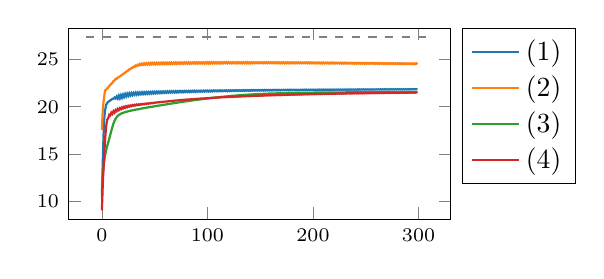
\begin{tikzpicture}

\definecolor{crimson2143940}{RGB}{214,39,40}
\definecolor{darkgray176}{RGB}{176,176,176}
\definecolor{darkorange25512714}{RGB}{255,127,14}
\definecolor{forestgreen4416044}{RGB}{44,160,44}
\definecolor{steelblue31119180}{RGB}{31,119,180}

\begin{axis}[compar, legend pos=outer north east]
\addplot [thick, steelblue31119180]
table {%
0 10.3699998855591
1 14.7799997329712
2 18.4699993133545
3 19.5900001525879
4 20.2000007629395
5 20.3899993896484
6 20.5200004577637
7 20.5900001525879
8 20.6900005340576
9 20.7399997711182
10 20.8500003814697
11 20.8400001525879
12 20.9799995422363
13 20.8899993896484
14 21.0900001525879
15 20.8899993896484
16 21.1700000762939
17 20.9099998474121
18 21.2199993133545
19 20.9699993133545
20 21.2800006866455
21 21.0499992370605
22 21.3400001525879
23 21.1100006103516
24 21.3899993896484
25 21.1700000762939
26 21.4300003051758
27 21.2199993133545
28 21.4500007629395
29 21.25
30 21.4699993133545
31 21.2800006866455
32 21.4899997711182
33 21.2999992370605
34 21.5100002288818
35 21.3199996948242
36 21.5200004577637
37 21.3400001525879
38 21.5300006866455
39 21.3500003814697
40 21.5400009155273
41 21.3700008392334
42 21.5499992370605
43 21.3799991607666
44 21.5599994659424
45 21.3999996185303
46 21.5699996948242
47 21.4099998474121
48 21.5799999237061
49 21.4200000762939
50 21.5900001525879
51 21.4400005340576
52 21.6000003814697
53 21.4500007629395
54 21.6100006103516
55 21.4599990844727
56 21.6100006103516
57 21.4699993133545
58 21.6200008392334
59 21.4799995422363
60 21.6299991607666
61 21.4899997711182
62 21.6299991607666
63 21.5
64 21.6399993896484
65 21.5100002288818
66 21.6499996185303
67 21.5200004577637
68 21.6499996185303
69 21.5200004577637
70 21.6599998474121
71 21.5300006866455
72 21.6599998474121
73 21.5400009155273
74 21.6700000762939
75 21.5499992370605
76 21.6700000762939
77 21.5499992370605
78 21.6800003051758
79 21.5599994659424
80 21.6800003051758
81 21.5699996948242
82 21.6800003051758
83 21.5699996948242
84 21.6900005340576
85 21.5799999237061
86 21.6900005340576
87 21.5900001525879
88 21.7000007629395
89 21.5900001525879
90 21.7000007629395
91 21.6000003814697
92 21.7000007629395
93 21.6000003814697
94 21.7099990844727
95 21.6100006103516
96 21.7099990844727
97 21.6100006103516
98 21.7099990844727
99 21.6200008392334
100 21.7199993133545
101 21.6200008392334
102 21.7199993133545
103 21.6299991607666
104 21.7199993133545
105 21.6299991607666
106 21.7299995422363
107 21.6399993896484
108 21.7299995422363
109 21.6399993896484
110 21.7299995422363
111 21.6499996185303
112 21.7399997711182
113 21.6499996185303
114 21.7399997711182
115 21.6599998474121
116 21.7399997711182
117 21.6599998474121
118 21.75
119 21.6599998474121
120 21.75
121 21.6700000762939
122 21.75
123 21.6700000762939
124 21.75
125 21.6800003051758
126 21.7600002288818
127 21.6800003051758
128 21.7600002288818
129 21.6800003051758
130 21.7600002288818
131 21.6900005340576
132 21.7600002288818
133 21.6900005340576
134 21.7700004577637
135 21.6900005340576
136 21.7700004577637
137 21.7000007629395
138 21.7700004577637
139 21.7000007629395
140 21.7700004577637
141 21.7000007629395
142 21.7800006866455
143 21.7099990844727
144 21.7800006866455
145 21.7099990844727
146 21.7800006866455
147 21.7099990844727
148 21.7800006866455
149 21.7199993133545
150 21.7800006866455
151 21.7199993133545
152 21.7900009155273
153 21.7199993133545
154 21.7900009155273
155 21.7199993133545
156 21.7900009155273
157 21.7299995422363
158 21.7900009155273
159 21.7299995422363
160 21.7900009155273
161 21.7299995422363
162 21.7900009155273
163 21.7399997711182
164 21.7999992370605
165 21.7399997711182
166 21.7999992370605
167 21.7399997711182
168 21.7999992370605
169 21.7399997711182
170 21.7999992370605
171 21.75
172 21.7999992370605
173 21.75
174 21.7999992370605
175 21.75
176 21.8099994659424
177 21.75
178 21.8099994659424
179 21.75
180 21.8099994659424
181 21.7600002288818
182 21.8099994659424
183 21.7600002288818
184 21.8099994659424
185 21.7600002288818
186 21.8099994659424
187 21.7600002288818
188 21.8099994659424
189 21.7700004577637
190 21.8199996948242
191 21.7700004577637
192 21.8199996948242
193 21.7700004577637
194 21.8199996948242
195 21.7700004577637
196 21.8199996948242
197 21.7700004577637
198 21.8199996948242
199 21.7800006866455
200 21.8199996948242
201 21.7800006866455
202 21.8199996948242
203 21.7800006866455
204 21.8199996948242
205 21.7800006866455
206 21.8299999237061
207 21.7800006866455
208 21.8299999237061
209 21.7800006866455
210 21.8299999237061
211 21.7900009155273
212 21.8299999237061
213 21.7900009155273
214 21.8299999237061
215 21.7900009155273
216 21.8299999237061
217 21.7900009155273
218 21.8299999237061
219 21.7900009155273
220 21.8299999237061
221 21.7999992370605
222 21.8299999237061
223 21.7999992370605
224 21.8400001525879
225 21.7999992370605
226 21.8400001525879
227 21.7999992370605
228 21.8400001525879
229 21.7999992370605
230 21.8400001525879
231 21.7999992370605
232 21.8400001525879
233 21.8099994659424
234 21.8400001525879
235 21.8099994659424
236 21.8400001525879
237 21.8099994659424
238 21.8400001525879
239 21.8099994659424
240 21.8400001525879
241 21.8099994659424
242 21.8500003814697
243 21.8099994659424
244 21.8500003814697
245 21.8199996948242
246 21.8500003814697
247 21.8199996948242
248 21.8500003814697
249 21.8199996948242
250 21.8500003814697
251 21.8199996948242
252 21.8500003814697
253 21.8199996948242
254 21.8500003814697
255 21.8199996948242
256 21.8500003814697
257 21.8199996948242
258 21.8500003814697
259 21.8299999237061
260 21.8500003814697
261 21.8299999237061
262 21.8600006103516
263 21.8299999237061
264 21.8600006103516
265 21.8299999237061
266 21.8600006103516
267 21.8299999237061
268 21.8600006103516
269 21.8299999237061
270 21.8600006103516
271 21.8299999237061
272 21.8600006103516
273 21.8299999237061
274 21.8600006103516
275 21.8400001525879
276 21.8600006103516
277 21.8400001525879
278 21.8600006103516
279 21.8400001525879
280 21.8600006103516
281 21.8400001525879
282 21.8600006103516
283 21.8400001525879
284 21.8600006103516
285 21.8400001525879
286 21.8600006103516
287 21.8400001525879
288 21.8600006103516
289 21.8400001525879
290 21.8600006103516
291 21.8400001525879
292 21.8700008392334
293 21.8400001525879
294 21.8700008392334
295 21.8500003814697
296 21.8700008392334
297 21.8500003814697
298 21.8700008392334
299 21.8500003814697
};
\addlegendentry{$(1)$}
\addplot [thick, darkorange25512714]
table {%
0 17.5499992370605
1 19.9500007629395
2 20.9200000762939
3 21.7399997711182
4 21.7999992370605
5 21.9699993133545
6 22.0200004577637
7 22.2199993133545
8 22.3099994659424
9 22.4699993133545
10 22.5300006866455
11 22.7399997711182
12 22.7800006866455
13 22.9699993133545
14 22.9699993133545
15 23.1100006103516
16 23.1299991607666
17 23.2399997711182
18 23.2999992370605
19 23.3899993896484
20 23.4699993133545
21 23.5400009155273
22 23.6399993896484
23 23.6900005340576
24 23.8199996948242
25 23.8400001525879
26 23.9799995422363
27 23.9899997711182
28 24.1399993896484
29 24.1200008392334
30 24.2700004577637
31 24.2299995422363
32 24.3799991607666
33 24.3199996948242
34 24.4699993133545
35 24.3899993896484
36 24.5400009155273
37 24.4300003051758
38 24.5799999237061
39 24.4599990844727
40 24.6100006103516
41 24.4799995422363
42 24.6299991607666
43 24.4899997711182
44 24.6399993896484
45 24.5
46 24.6499996185303
47 24.5100002288818
48 24.6599998474121
49 24.5200004577637
50 24.6599998474121
51 24.5200004577637
52 24.6700000762939
53 24.5300006866455
54 24.6700000762939
55 24.5300006866455
56 24.6700000762939
57 24.5400009155273
58 24.6800003051758
59 24.5400009155273
60 24.6800003051758
61 24.5400009155273
62 24.6800003051758
63 24.5499992370605
64 24.6900005340576
65 24.5499992370605
66 24.6900005340576
67 24.5599994659424
68 24.6900005340576
69 24.5599994659424
70 24.7000007629395
71 24.5599994659424
72 24.7000007629395
73 24.5699996948242
74 24.7000007629395
75 24.5699996948242
76 24.7000007629395
77 24.5699996948242
78 24.7099990844727
79 24.5799999237061
80 24.7099990844727
81 24.5799999237061
82 24.7099990844727
83 24.5799999237061
84 24.7099990844727
85 24.5900001525879
86 24.7099990844727
87 24.5900001525879
88 24.7199993133545
89 24.5900001525879
90 24.7199993133545
91 24.5900001525879
92 24.7199993133545
93 24.6000003814697
94 24.7199993133545
95 24.6000003814697
96 24.7199993133545
97 24.6000003814697
98 24.7199993133545
99 24.6000003814697
100 24.7299995422363
101 24.6000003814697
102 24.7299995422363
103 24.6100006103516
104 24.7299995422363
105 24.6100006103516
106 24.7299995422363
107 24.6100006103516
108 24.7299995422363
109 24.6100006103516
110 24.7299995422363
111 24.6100006103516
112 24.7299995422363
113 24.6100006103516
114 24.7299995422363
115 24.6100006103516
116 24.7299995422363
117 24.6200008392334
118 24.7299995422363
119 24.6200008392334
120 24.7299995422363
121 24.6200008392334
122 24.7299995422363
123 24.6200008392334
124 24.7299995422363
125 24.6200008392334
126 24.7299995422363
127 24.6200008392334
128 24.7299995422363
129 24.6200008392334
130 24.7299995422363
131 24.6200008392334
132 24.7299995422363
133 24.6200008392334
134 24.7299995422363
135 24.6200008392334
136 24.7299995422363
137 24.6200008392334
138 24.7299995422363
139 24.6200008392334
140 24.7299995422363
141 24.6200008392334
142 24.7299995422363
143 24.6299991607666
144 24.7299995422363
145 24.6299991607666
146 24.7299995422363
147 24.6299991607666
148 24.7299995422363
149 24.6299991607666
150 24.7299995422363
151 24.6299991607666
152 24.7299995422363
153 24.6299991607666
154 24.7299995422363
155 24.6299991607666
156 24.7299995422363
157 24.6299991607666
158 24.7299995422363
159 24.6299991607666
160 24.7299995422363
161 24.6299991607666
162 24.7299995422363
163 24.6299991607666
164 24.7299995422363
165 24.6299991607666
166 24.7299995422363
167 24.6200008392334
168 24.7199993133545
169 24.6200008392334
170 24.7199993133545
171 24.6200008392334
172 24.7199993133545
173 24.6200008392334
174 24.7199993133545
175 24.6200008392334
176 24.7199993133545
177 24.6200008392334
178 24.7199993133545
179 24.6200008392334
180 24.7199993133545
181 24.6200008392334
182 24.7199993133545
183 24.6200008392334
184 24.7199993133545
185 24.6200008392334
186 24.7099990844727
187 24.6200008392334
188 24.7099990844727
189 24.6200008392334
190 24.7099990844727
191 24.6200008392334
192 24.7099990844727
193 24.6200008392334
194 24.7099990844727
195 24.6200008392334
196 24.7099990844727
197 24.6100006103516
198 24.7099990844727
199 24.6100006103516
200 24.7000007629395
201 24.6100006103516
202 24.7000007629395
203 24.6100006103516
204 24.7000007629395
205 24.6100006103516
206 24.7000007629395
207 24.6100006103516
208 24.7000007629395
209 24.6100006103516
210 24.7000007629395
211 24.6100006103516
212 24.6900005340576
213 24.6100006103516
214 24.6900005340576
215 24.6000003814697
216 24.6900005340576
217 24.6000003814697
218 24.6900005340576
219 24.6000003814697
220 24.6900005340576
221 24.6000003814697
222 24.6800003051758
223 24.6000003814697
224 24.6800003051758
225 24.6000003814697
226 24.6800003051758
227 24.5900001525879
228 24.6800003051758
229 24.5900001525879
230 24.6800003051758
231 24.5900001525879
232 24.6700000762939
233 24.5900001525879
234 24.6700000762939
235 24.5900001525879
236 24.6700000762939
237 24.5900001525879
238 24.6700000762939
239 24.5799999237061
240 24.6700000762939
241 24.5799999237061
242 24.6599998474121
243 24.5799999237061
244 24.6599998474121
245 24.5799999237061
246 24.6599998474121
247 24.5799999237061
248 24.6599998474121
249 24.5699996948242
250 24.6499996185303
251 24.5699996948242
252 24.6499996185303
253 24.5699996948242
254 24.6499996185303
255 24.5699996948242
256 24.6499996185303
257 24.5699996948242
258 24.6499996185303
259 24.5599994659424
260 24.6399993896484
261 24.5599994659424
262 24.6399993896484
263 24.5599994659424
264 24.6399993896484
265 24.5599994659424
266 24.6399993896484
267 24.5599994659424
268 24.6299991607666
269 24.5499992370605
270 24.6299991607666
271 24.5499992370605
272 24.6299991607666
273 24.5499992370605
274 24.6299991607666
275 24.5499992370605
276 24.6299991607666
277 24.5499992370605
278 24.6200008392334
279 24.5499992370605
280 24.6200008392334
281 24.5400009155273
282 24.6200008392334
283 24.5400009155273
284 24.6200008392334
285 24.5400009155273
286 24.6200008392334
287 24.5400009155273
288 24.6100006103516
289 24.5400009155273
290 24.6100006103516
291 24.5400009155273
292 24.6100006103516
293 24.5300006866455
294 24.6100006103516
295 24.5300006866455
296 24.6100006103516
297 24.5300006866455
298 24.6100006103516
299 24.5300006866455
};
\addlegendentry{$(2)$}
\addplot [thick, forestgreen4416044]
table {%
0 11.539999961853
1 12.9200000762939
2 14.039999961853
3 14.8100004196167
4 15.3599996566772
5 15.8000001907349
7 16.6200008392334
9 17.4599990844727
10 17.8600006103516
11 18.2299995422363
12 18.5100002288818
13 18.7299995422363
14 18.8899993896484
15 19.0200004577637
16 19.1200008392334
18 19.2600002288818
19 19.3099994659424
22 19.4300003051758
26 19.5499992370605
27 19.5699996948242
28 19.6000003814697
30 19.6399993896484
31 19.6700000762939
36 19.7700004577637
37 19.7999992370605
45 19.9599990844727
46 19.9699993133545
54 20.1299991607666
55 20.1399993896484
59 20.2199993133545
60 20.2299995422363
64 20.3099994659424
65 20.3199996948242
68 20.3799991607666
69 20.3899993896484
72 20.4500007629395
73 20.4599990844727
75 20.5
76 20.5100002288818
78 20.5499992370605
79 20.5599994659424
81 20.6000003814697
82 20.6100006103516
83 20.6299991607666
84 20.6399993896484
86 20.6800003051758
87 20.6900005340576
88 20.7099990844727
89 20.7199993133545
90 20.7399997711182
91 20.75
92 20.7700004577637
93 20.7800006866455
94 20.7999992370605
95 20.8099994659424
96 20.8299999237061
98 20.8500003814697
99 20.8700008392334
101 20.8899993896484
102 20.9099998474121
104 20.9300003051758
105 20.9500007629395
107 20.9699993133545
108 20.9899997711182
112 21.0300006866455
113 21.0499992370605
121 21.1299991607666
122 21.1499996185303
123 21.1599998474121
124 21.1599998474121
133 21.25
134 21.25
137 21.2800006866455
138 21.2800006866455
140 21.2999992370605
141 21.2999992370605
143 21.3199996948242
144 21.3199996948242
146 21.3400001525879
147 21.3400001525879
148 21.3500003814697
149 21.3500003814697
150 21.3600006103516
151 21.3600006103516
152 21.3700008392334
153 21.3700008392334
154 21.3799991607666
155 21.3799991607666
156 21.3899993896484
157 21.3899993896484
158 21.3999996185303
160 21.3999996185303
161 21.4099998474121
162 21.4099998474121
163 21.4200000762939
165 21.4200000762939
166 21.4300003051758
168 21.4300003051758
169 21.4400005340576
171 21.4400005340576
172 21.4500007629395
175 21.4500007629395
176 21.4599990844727
178 21.4599990844727
179 21.4699993133545
183 21.4699993133545
184 21.4799995422363
188 21.4799995422363
189 21.4899997711182
193 21.4899997711182
194 21.5
200 21.5
201 21.5100002288818
208 21.5100002288818
209 21.5200004577637
218 21.5200004577637
219 21.5300006866455
231 21.5300006866455
232 21.5400009155273
246 21.5400009155273
247 21.5499992370605
262 21.5499992370605
263 21.5599994659424
279 21.5599994659424
280 21.5699996948242
295 21.5699996948242
296 21.5799999237061
299 21.5799999237061
};
\addlegendentry{$(3)$}
\addplot [thick, crimson2143940]
table {%
0 8.97999954223633
1 12.210000038147
2 14.4200000762939
3 16.4699993133545
4 17.8700008392334
5 18.6299991607666
6 18.7700004577637
7 19.1499996185303
8 19.0799999237061
9 19.3799991607666
10 19.2399997711182
11 19.5300006866455
12 19.3799991607666
13 19.6499996185303
14 19.5300006866455
15 19.7600002288818
16 19.6399993896484
17 19.8500003814697
18 19.7399997711182
19 19.9300003051758
20 19.8199996948242
21 20
22 19.8899993896484
23 20.0499992370605
24 19.9500007629395
25 20.1000003814697
26 20.0100002288818
27 20.1399993896484
28 20.0599994659424
29 20.1800003051758
30 20.1000003814697
31 20.2099990844727
32 20.1399993896484
33 20.2399997711182
34 20.1700000762939
35 20.2600002288818
36 20.2000007629395
37 20.2900009155273
38 20.2299995422363
39 20.3099994659424
40 20.2600002288818
41 20.3299999237061
42 20.2900009155273
43 20.3600006103516
44 20.3199996948242
45 20.3799991607666
46 20.3500003814697
47 20.4099998474121
48 20.3799991607666
49 20.4300003051758
50 20.4099998474121
51 20.4500007629395
52 20.4400005340576
53 20.4799995422363
54 20.4599990844727
55 20.5
56 20.4899997711182
57 20.5200004577637
58 20.5100002288818
59 20.5499992370605
60 20.5400009155273
61 20.5699996948242
62 20.5599994659424
63 20.5900001525879
64 20.5900001525879
65 20.6100006103516
66 20.6100006103516
67 20.6299991607666
68 20.6299991607666
69 20.6499996185303
78 20.7399997711182
79 20.7399997711182
80 20.7600002288818
81 20.7600002288818
82 20.7800006866455
83 20.7800006866455
84 20.7900009155273
85 20.7900009155273
86 20.8099994659424
87 20.8099994659424
88 20.8299999237061
89 20.8199996948242
90 20.8500003814697
91 20.8400001525879
92 20.8600006103516
93 20.8500003814697
94 20.8799991607666
95 20.8700008392334
96 20.8899993896484
97 20.8799991607666
98 20.9099998474121
99 20.8999996185303
100 20.9200000762939
101 20.9099998474121
102 20.9400005340576
103 20.9200000762939
104 20.9500007629395
105 20.9400005340576
106 20.9699993133545
107 20.9500007629395
108 20.9799995422363
109 20.9599990844727
110 20.9899997711182
111 20.9699993133545
112 21.0100002288818
113 20.9899997711182
114 21.0200004577637
115 21
116 21.0300006866455
117 21.0100002288818
118 21.0400009155273
119 21.0200004577637
120 21.0599994659424
121 21.0300006866455
122 21.0699996948242
123 21.0400009155273
124 21.0799999237061
125 21.0499992370605
126 21.0900001525879
127 21.0599994659424
128 21.1000003814697
129 21.0699996948242
130 21.1100006103516
131 21.0799999237061
132 21.1200008392334
133 21.0900001525879
134 21.1299991607666
135 21.1000003814697
136 21.1399993896484
137 21.1100006103516
138 21.1499996185303
139 21.1200008392334
140 21.1599998474121
141 21.1299991607666
142 21.1700000762939
143 21.1399993896484
144 21.1800003051758
145 21.1499996185303
146 21.1800003051758
147 21.1499996185303
148 21.1900005340576
149 21.1599998474121
150 21.2000007629395
151 21.1700000762939
152 21.2099990844727
153 21.1800003051758
154 21.2199993133545
155 21.1900005340576
156 21.2199993133545
157 21.1900005340576
158 21.2299995422363
159 21.2000007629395
160 21.2399997711182
161 21.2099990844727
162 21.25
163 21.2099990844727
164 21.25
165 21.2199993133545
166 21.2600002288818
167 21.2299995422363
168 21.2700004577637
169 21.2299995422363
170 21.2700004577637
171 21.2399997711182
172 21.2800006866455
173 21.25
174 21.2900009155273
175 21.25
176 21.2900009155273
177 21.2600002288818
178 21.2999992370605
179 21.2700004577637
180 21.3099994659424
181 21.2700004577637
182 21.3099994659424
183 21.2800006866455
184 21.3199996948242
185 21.2800006866455
186 21.3199996948242
187 21.2900009155273
188 21.3299999237061
189 21.2900009155273
190 21.3299999237061
191 21.2999992370605
192 21.3400001525879
193 21.3099994659424
194 21.3400001525879
195 21.3099994659424
196 21.3500003814697
197 21.3199996948242
198 21.3500003814697
199 21.3199996948242
200 21.3600006103516
201 21.3299999237061
202 21.3600006103516
203 21.3299999237061
204 21.3700008392334
205 21.3400001525879
206 21.3700008392334
207 21.3400001525879
208 21.3799991607666
209 21.3400001525879
210 21.3799991607666
211 21.3500003814697
212 21.3899993896484
213 21.3500003814697
214 21.3899993896484
215 21.3600006103516
216 21.3999996185303
217 21.3600006103516
218 21.3999996185303
219 21.3700008392334
220 21.3999996185303
221 21.3700008392334
222 21.4099998474121
223 21.3799991607666
224 21.4099998474121
225 21.3799991607666
226 21.4200000762939
227 21.3799991607666
228 21.4200000762939
229 21.3899993896484
230 21.4200000762939
231 21.3899993896484
232 21.4300003051758
233 21.3999996185303
234 21.4300003051758
235 21.3999996185303
236 21.4300003051758
237 21.3999996185303
238 21.4400005340576
239 21.4099998474121
240 21.4400005340576
241 21.4099998474121
242 21.4400005340576
243 21.4099998474121
244 21.4500007629395
245 21.4200000762939
246 21.4500007629395
247 21.4200000762939
248 21.4500007629395
249 21.4200000762939
250 21.4599990844727
251 21.4300003051758
252 21.4599990844727
253 21.4300003051758
254 21.4599990844727
255 21.4300003051758
256 21.4699993133545
257 21.4400005340576
258 21.4699993133545
259 21.4400005340576
260 21.4699993133545
261 21.4400005340576
262 21.4799995422363
263 21.4500007629395
264 21.4799995422363
265 21.4500007629395
266 21.4799995422363
267 21.4500007629395
268 21.4899997711182
269 21.4599990844727
270 21.4899997711182
271 21.4599990844727
272 21.4899997711182
273 21.4599990844727
274 21.4899997711182
275 21.4699993133545
276 21.5
277 21.4699993133545
278 21.5
279 21.4699993133545
280 21.5
281 21.4699993133545
282 21.5
283 21.4799995422363
284 21.5100002288818
285 21.4799995422363
286 21.5100002288818
287 21.4799995422363
288 21.5100002288818
289 21.4799995422363
290 21.5100002288818
291 21.4899997711182
292 21.5200004577637
293 21.4899997711182
294 21.5200004577637
295 21.4899997711182
296 21.5200004577637
297 21.4899997711182
298 21.5200004577637
299 21.5
};
\addlegendentry{$(4)$}
\addplot [thick, gray, dashed]
table {%
-14.95 27.4213390350342
313.95 27.4213390350342
};
\end{axis}

\end{tikzpicture}
}
\end{tabular}
	\caption{$d=400$, sans passe-base}
	\label{fig:LGDlat400-s}
\end{figure}

\begin{figure}[H]\centering
	\begin{tabular}{c c c c c c}
	Target  &  $(1)$  &  $(2)$  &  $(3)$  &  $(4)$  &  $(5)$
	
	\\
	
	\multirow{3}{0.3\textwidth}[0.05\textwidth]{\includegraphics[width=0.3\textwidth]{resultats/LGD/sizes/size-target-g.png}}
	&
	\includegraphics[width=0.12\textwidth]{resultats/LGD/sizes/size_big-init-pas=0.2_filtre=g-0.6.png}
	&
	\includegraphics[width=0.12\textwidth]{resultats/LGD/sizes/size_mid2-init-pas=0.1_filtre=g-0.6.png}
	&
	\includegraphics[width=0.12\textwidth]{resultats/LGD/sizes/size_mid1-init-pas=0.1_filtre=g-0.6.png}
	&
	\includegraphics[width=0.12\textwidth]{resultats/LGD/sizes/size_small-init-pas=0.5_filtre=g-0.6.png}
	&
	\includegraphics[width=0.12\textwidth]{resultats/LGD/sizes/size_mini-init-pas=0.01_filtre=g-0.6.png}
	
	\\
	
	
	&
	\includegraphics[width=0.12\textwidth]{resultats/LGD/sizes/size_big-compatarget-s.png}
	&
	\includegraphics[width=0.12\textwidth]{resultats/LGD/sizes/size_mid2-compatarget-s.png}
	&
	\includegraphics[height=0.12\textwidth]{resultats/LGD/sizes/size_mid1-compatarget-s.png}
	&
	\includegraphics[width=0.12\textwidth]{resultats/LGD/sizes/size_small-compatarget-s.png}
	&
	\includegraphics[width=0.12\textwidth]{resultats/LGD/sizes/size_mini-compatarget-s.png}
	
	\\
	
	
	&
	\includegraphics[width=0.12\textwidth]{resultats/LGD/sizes/size_big-guess-pas=0.2_filtre=g-0.6.png}
	&
	\includegraphics[width=0.12\textwidth]{resultats/LGD/sizes/size_mid2-guess-pas=0.1_filtre=g-0.6.png}
	&
	\includegraphics[width=0.12\textwidth]{resultats/LGD/sizes/size_mid1-guess-pas=0.1_filtre=g-0.6.png}
	&
	\includegraphics[width=0.12\textwidth]{resultats/LGD/sizes/size_small-guess-pas=0.5_filtre=g-0.6.png}
	&
	\includegraphics[width=0.12\textwidth]{resultats/LGD/sizes/size_mini-guess-pas=0.01_filtre=g-0.6.png}
	
	\\ \\
	
	
	
	\multicolumn{2}{c}{Loss}  &  \multicolumn{4}{c}{PSNR{\color{white}bbbb}}
	
	\\
	
	\multicolumn{2}{c}{% This file was created with tikzplotlib v0.10.1.
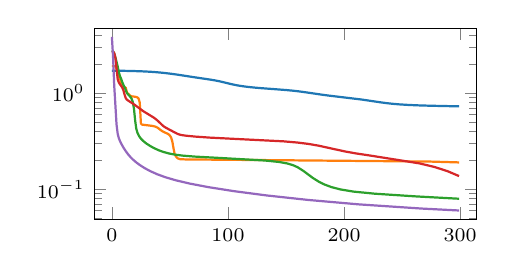
\begin{tikzpicture}

\definecolor{crimson2143940}{RGB}{214,39,40}
\definecolor{darkgray176}{RGB}{176,176,176}
\definecolor{darkorange25512714}{RGB}{255,127,14}
\definecolor{forestgreen4416044}{RGB}{44,160,44}
\definecolor{mediumpurple148103189}{RGB}{148,103,189}
\definecolor{steelblue31119180}{RGB}{31,119,180}

\begin{axis}[compar,
	ymode=log]
\addplot [thick, steelblue31119180]
table {%
0 1.72453677654266
10 1.71768462657928
18 1.709348320961
24 1.70033705234528
29 1.6901341676712
34 1.67662823200226
38 1.66295230388641
42 1.64652991294861
46 1.62746405601501
51 1.60032224655151
56 1.5699542760849
63 1.52379190921783
70 1.47829067707062
76 1.44239723682404
86 1.38365793228149
90 1.35641014575958
93 1.33313751220703
97 1.29875993728638
102 1.25543904304504
105 1.23231077194214
108 1.2123007774353
111 1.19530928134918
114 1.18089818954468
118 1.16483271121979
123 1.14839255809784
129 1.13209295272827
138 1.11113858222961
150 1.08306062221527
156 1.06606793403625
161 1.0491931438446
167 1.02564668655396
181 0.968385457992554
187 0.947251319885254
195 0.922387599945068
215 0.862796425819397
224 0.831477165222168
232 0.804347276687622
237 0.789946675300598
242 0.778159737586975
248 0.767242193222046
255 0.757997989654541
263 0.75055992603302
274 0.743492960929871
293 0.734858512878418
299 0.732345581054688
};
\addplot [thick, darkorange25512714]
table {%
0 1.93434596061707
1 1.93200349807739
2 1.92700910568237
3 1.91092967987061
4 1.82279932498932
5 1.63814675807953
6 1.49781715869904
7 1.42523396015167
8 1.27939009666443
9 1.18521678447723
10 1.17097330093384
11 1.16010677814484
12 1.13860154151917
13 1.018106341362
16 0.941693305969238
17 0.931789517402649
20 0.922242164611816
21 0.916382789611816
22 0.905909538269043
23 0.883619070053101
24 0.800576210021973
25 0.484217882156372
26 0.472478270530701
35 0.457828998565674
37 0.451737642288208
38 0.44725227355957
39 0.441246032714844
40 0.433329820632935
42 0.41453742980957
44 0.39980947971344
46 0.389489531517029
48 0.379505157470703
49 0.372840166091919
50 0.363147974014282
51 0.346918106079102
52 0.317295432090759
53 0.271204471588135
54 0.234548449516296
55 0.221139311790466
56 0.213874220848083
57 0.209440231323242
59 0.205981850624084
64 0.20487642288208
108 0.202854156494141
273 0.194810152053833
297 0.191097617149353
299 0.190571308135986
};
\addplot [thick, forestgreen4416044]
table {%
0 2.80895972251892
1 2.75048971176147
2 2.60713028907776
3 2.38255786895752
4 2.13562965393066
5 1.91229856014252
6 1.65637183189392
7 1.50856399536133
8 1.41280651092529
9 1.30485808849335
10 1.22169101238251
11 1.15476989746094
12 1.0741560459137
13 1.00716495513916
14 0.973587155342102
15 0.946269989013672
16 0.916436076164246
17 0.876654148101807
18 0.812723636627197
19 0.697008371353149
20 0.525444269180298
21 0.428455829620361
22 0.389726042747498
23 0.366618156433105
24 0.350306034088135
25 0.337761163711548
26 0.32756519317627
28 0.311413407325745
30 0.298583030700684
33 0.282851934432983
36 0.269976496696472
40 0.256317496299744
44 0.245958089828491
49 0.236628293991089
54 0.230266451835632
61 0.224518775939941
71 0.219510316848755
92 0.2126624584198
132 0.199638366699219
144 0.192842841148376
151 0.186120629310608
156 0.178535461425781
160 0.169811010360718
165 0.155425310134888
173 0.131635665893555
178 0.120536088943481
183 0.112421870231628
189 0.10558009147644
197 0.0996513366699219
208 0.0947535037994385
226 0.0901226997375488
262 0.0843832492828369
299 0.0798095464706421
};
\addplot [thick, crimson2143940]
table {%
0 2.75355887413025
1 2.72030234336853
2 2.63165354728699
3 2.34783864021301
4 1.81270730495453
5 1.40633320808411
6 1.2964209318161
7 1.23945200443268
8 1.19617938995361
9 1.146324634552
10 1.06876111030579
11 0.963654279708862
12 0.885666608810425
13 0.858596682548523
14 0.841736435890198
20 0.754436254501343
24 0.694417476654053
26 0.666041374206543
28 0.641217947006226
30 0.620044827461243
36 0.559826135635376
38 0.536990165710449
40 0.511477112770081
43 0.471526265144348
44 0.459928154945374
45 0.450082421302795
47 0.435087561607361
56 0.381032824516296
58 0.372854471206665
60 0.367727637290955
64 0.361920237541199
72 0.354321241378784
84 0.346086740493774
101 0.337772607803345
148 0.316205859184265
160 0.30713939666748
169 0.297676563262939
178 0.285158157348633
191 0.26324725151062
201 0.247857093811035
210 0.236915230751038
223 0.224390149116516
265 0.186241030693054
278 0.17077362537384
289 0.154715538024902
299 0.137419939041138
};
\addplot [thick, mediumpurple148103189]
table {%
0 3.87609815597534
1 2.41971015930176
2 1.21478092670441
3 0.759954929351807
4 0.473417043685913
5 0.378544330596924
6 0.340376138687134
7 0.318324327468872
8 0.300664186477661
9 0.285422086715698
10 0.271982550621033
12 0.249404191970825
14 0.231428861618042
16 0.216980695724487
18 0.205150842666626
21 0.190834045410156
24 0.179333209991455
28 0.166966199874878
33 0.154839515686035
39 0.143672823905945
46 0.133790850639343
55 0.124259471893311
67 0.114835143089294
83 0.105466246604919
105 0.0957608222961426
133 0.0864417552947998
169 0.0775313377380371
213 0.0696594715118408
267 0.0630255937576294
299 0.0601816177368164
};
\end{axis}

\end{tikzpicture}
}
	&
	\multicolumn{4}{c}{% This file was created with tikzplotlib v0.10.1.
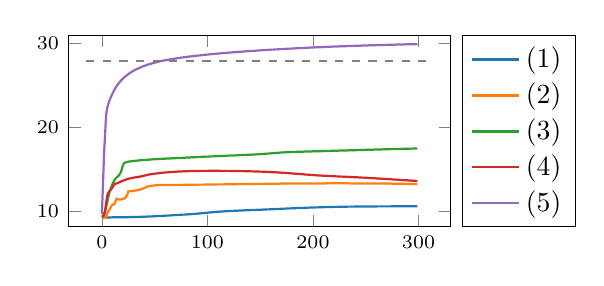
\begin{tikzpicture}

\definecolor{crimson2143940}{RGB}{214,39,40}
\definecolor{darkgray176}{RGB}{176,176,176}
\definecolor{darkorange25512714}{RGB}{255,127,14}
\definecolor{forestgreen4416044}{RGB}{44,160,44}
\definecolor{mediumpurple148103189}{RGB}{148,103,189}
\definecolor{steelblue31119180}{RGB}{31,119,180}

\begin{axis}[compar, legend pos=outer north east]
\addplot [thick, steelblue31119180]
table {%
0 9.31999969482422
9 9.31999969482422
10 9.32999992370605
17 9.32999992370605
18 9.34000015258789
22 9.34000015258789
23 9.35000038146973
26 9.35000038146973
27 9.35999965667725
30 9.35999965667725
31 9.36999988555908
33 9.36999988555908
34 9.38000011444092
36 9.38000011444092
37 9.39000034332275
38 9.39000034332275
39 9.39999961853027
40 9.39999961853027
41 9.40999984741211
42 9.40999984741211
43 9.42000007629395
44 9.42000007629395
45 9.43000030517578
46 9.43000030517578
47 9.4399995803833
48 9.4399995803833
49 9.44999980926514
50 9.44999980926514
52 9.47000026702881
53 9.47000026702881
55 9.48999977111816
56 9.48999977111816
58 9.51000022888184
59 9.51000022888184
61 9.52999973297119
62 9.52999973297119
65 9.5600004196167
66 9.5600004196167
69 9.59000015258789
70 9.59000015258789
73 9.61999988555908
74 9.61999988555908
77 9.64999961853027
78 9.64999961853027
82 9.6899995803833
83 9.6899995803833
94 9.80000019073486
95 9.81999969482422
98 9.85000038146973
99 9.86999988555908
103 9.90999984741211
104 9.93000030517578
112 10.0100002288818
113 10.0100002288818
117 10.0500001907349
118 10.0500001907349
120 10.0699996948242
121 10.0699996948242
123 10.0900001525879
124 10.0900001525879
126 10.1099996566772
127 10.1099996566772
128 10.1199998855591
129 10.1199998855591
130 10.1300001144409
131 10.1300001144409
133 10.1499996185303
134 10.1499996185303
135 10.1599998474121
136 10.1599998474121
137 10.1700000762939
138 10.1700000762939
139 10.1800003051758
140 10.1800003051758
141 10.1899995803833
142 10.1899995803833
143 10.1999998092651
144 10.1999998092651
145 10.210000038147
146 10.210000038147
147 10.2200002670288
148 10.2200002670288
149 10.2299995422363
150 10.2299995422363
151 10.2399997711182
152 10.2399997711182
153 10.25
154 10.25
155 10.2600002288818
156 10.2600002288818
157 10.2700004577637
158 10.2700004577637
159 10.2799997329712
160 10.2799997329712
161 10.289999961853
162 10.289999961853
164 10.3100004196167
165 10.3100004196167
166 10.3199996948242
167 10.3199996948242
168 10.3299999237061
169 10.3299999237061
171 10.3500003814697
172 10.3500003814697
173 10.3599996566772
174 10.3599996566772
175 10.3699998855591
176 10.3699998855591
178 10.3900003433228
179 10.3900003433228
180 10.3999996185303
181 10.3999996185303
182 10.4099998474121
183 10.4099998474121
184 10.4200000762939
185 10.4200000762939
186 10.4300003051758
187 10.4300003051758
188 10.4399995803833
189 10.4399995803833
190 10.4499998092651
191 10.4499998092651
192 10.460000038147
193 10.460000038147
194 10.4700002670288
195 10.4700002670288
196 10.4799995422363
197 10.4799995422363
198 10.4899997711182
200 10.4899997711182
201 10.5
202 10.5
203 10.5100002288818
205 10.5100002288818
206 10.5200004577637
207 10.5200004577637
208 10.5299997329712
210 10.5299997329712
211 10.539999961853
213 10.539999961853
214 10.5500001907349
216 10.5500001907349
217 10.5600004196167
219 10.5600004196167
220 10.5699996948242
223 10.5699996948242
224 10.5799999237061
227 10.5799999237061
228 10.5900001525879
232 10.5900001525879
233 10.6000003814697
239 10.6000003814697
240 10.6099996566772
248 10.6099996566772
249 10.6199998855591
260 10.6199998855591
261 10.6300001144409
274 10.6300001144409
275 10.6400003433228
287 10.6400003433228
288 10.6499996185303
299 10.6499996185303
};
\addlegendentry{$(1)$}
\addplot [thick, darkorange25512714]
table {%
0 9.28999996185303
1 9.28999996185303
2 9.30000019073486
3 9.31999969482422
4 9.4399995803833
5 9.73999977111816
6 10.0600004196167
7 10.1899995803833
8 10.4499998092651
9 10.6599998474121
10 10.8100004196167
11 10.8400001525879
12 10.9200000762939
13 11.2200002670288
14 11.5500001907349
15 11.5100002288818
16 11.460000038147
17 11.4399995803833
18 11.460000038147
19 11.4700002670288
20 11.5100002288818
21 11.5600004196167
22 11.6400003433228
23 11.75
24 12.0100002288818
25 12.3999996185303
26 12.4099998474121
27 12.4499998092651
28 12.4300003051758
29 12.4700002670288
30 12.460000038147
31 12.5
32 12.5
33 12.539999961853
34 12.5500001907349
35 12.5900001525879
36 12.6099996566772
37 12.6599998474121
38 12.6899995803833
40 12.789999961853
41 12.8599996566772
43 12.960000038147
44 13
45 13.0200004577637
46 13.0500001907349
47 13.0699996948242
48 13.0799999237061
50 13.1199998855591
51 13.1300001144409
52 13.1499996185303
53 13.1499996185303
54 13.1599998474121
60 13.1599998474121
61 13.1700000762939
69 13.1700000762939
70 13.1800003051758
77 13.1800003051758
78 13.1899995803833
84 13.1899995803833
85 13.1999998092651
91 13.1999998092651
92 13.210000038147
97 13.210000038147
98 13.2200002670288
104 13.2200002670288
105 13.2299995422363
109 13.2299995422363
110 13.2399997711182
115 13.2399997711182
116 13.25
121 13.25
122 13.2600002288818
127 13.2600002288818
128 13.2700004577637
133 13.2700004577637
134 13.2799997329712
139 13.2799997329712
140 13.289999961853
146 13.289999961853
147 13.3000001907349
153 13.3000001907349
154 13.3100004196167
160 13.3100004196167
161 13.3199996948242
168 13.3199996948242
169 13.3299999237061
178 13.3299999237061
179 13.3400001525879
190 13.3400001525879
191 13.3500003814697
211 13.3500003814697
212 13.3599996566772
234 13.3599996566772
235 13.3500003814697
255 13.3500003814697
256 13.3400001525879
266 13.3400001525879
267 13.3299999237061
274 13.3299999237061
275 13.3199996948242
280 13.3199996948242
281 13.3100004196167
285 13.3100004196167
286 13.3000001907349
289 13.3000001907349
290 13.289999961853
293 13.289999961853
294 13.2799997329712
296 13.2799997329712
297 13.2700004577637
299 13.2700004577637
};
\addlegendentry{$(2)$}
\addplot [thick, forestgreen4416044]
table {%
0 9.39999961853027
1 9.48999977111816
2 9.69999980926514
3 10.0799999237061
4 10.539999961853
5 11.039999961853
6 11.6999998092651
7 12.1999998092651
8 12.5699996948242
9 12.9499998092651
10 13.2600002288818
12 13.7399997711182
13 13.9399995803833
14 14.0600004196167
15 14.1700000762939
16 14.289999961853
17 14.460000038147
18 14.710000038147
19 15.0900001525879
20 15.5299997329712
21 15.7399997711182
22 15.8199996948242
23 15.8699998855591
25 15.9300003051758
27 15.9700002670288
28 15.9799995422363
29 16
30 16.0100002288818
31 16.0300006866455
33 16.0499992370605
34 16.0699996948242
48 16.2099990844727
49 16.2099990844727
52 16.2399997711182
53 16.2399997711182
55 16.2600002288818
56 16.2600002288818
58 16.2800006866455
59 16.2800006866455
61 16.2999992370605
62 16.2999992370605
63 16.3099994659424
64 16.3099994659424
66 16.3299999237061
67 16.3299999237061
69 16.3500003814697
70 16.3500003814697
72 16.3700008392334
73 16.3700008392334
74 16.3799991607666
75 16.3799991607666
77 16.3999996185303
78 16.3999996185303
80 16.4200000762939
81 16.4200000762939
82 16.4300003051758
83 16.4300003051758
85 16.4500007629395
86 16.4500007629395
87 16.4599990844727
88 16.4599990844727
90 16.4799995422363
91 16.4799995422363
92 16.4899997711182
93 16.4899997711182
95 16.5100002288818
96 16.5100002288818
97 16.5200004577637
98 16.5200004577637
99 16.5300006866455
100 16.5300006866455
102 16.5499992370605
103 16.5499992370605
104 16.5599994659424
105 16.5599994659424
106 16.5699996948242
107 16.5699996948242
109 16.5900001525879
110 16.5900001525879
111 16.6000003814697
112 16.6000003814697
113 16.6100006103516
114 16.6100006103516
115 16.6200008392334
116 16.6200008392334
118 16.6399993896484
119 16.6399993896484
120 16.6499996185303
121 16.6499996185303
122 16.6599998474121
123 16.6599998474121
124 16.6700000762939
125 16.6700000762939
126 16.6800003051758
127 16.6800003051758
129 16.7000007629395
130 16.7000007629395
131 16.7099990844727
132 16.7099990844727
133 16.7199993133545
134 16.7199993133545
135 16.7299995422363
136 16.7299995422363
138 16.75
139 16.75
140 16.7600002288818
141 16.7600002288818
143 16.7800006866455
144 16.7800006866455
146 16.7999992370605
147 16.7999992370605
150 16.8299999237061
151 16.8299999237061
169 17.0100002288818
170 17.0100002288818
173 17.0400009155273
174 17.0400009155273
176 17.0599994659424
177 17.0599994659424
178 17.0699996948242
179 17.0699996948242
180 17.0799999237061
181 17.0799999237061
182 17.0900001525879
183 17.0900001525879
184 17.1000003814697
186 17.1000003814697
187 17.1100006103516
188 17.1100006103516
189 17.1200008392334
191 17.1200008392334
192 17.1299991607666
194 17.1299991607666
195 17.1399993896484
197 17.1399993896484
198 17.1499996185303
199 17.1499996185303
200 17.1599998474121
202 17.1599998474121
203 17.1700000762939
205 17.1700000762939
206 17.1800003051758
208 17.1800003051758
209 17.1900005340576
211 17.1900005340576
212 17.2000007629395
214 17.2000007629395
215 17.2099990844727
216 17.2099990844727
217 17.2199993133545
219 17.2199993133545
220 17.2299995422363
222 17.2299995422363
223 17.2399997711182
224 17.2399997711182
225 17.25
227 17.25
228 17.2600002288818
230 17.2600002288818
231 17.2700004577637
233 17.2700004577637
234 17.2800006866455
235 17.2800006866455
236 17.2900009155273
238 17.2900009155273
239 17.2999992370605
241 17.2999992370605
242 17.3099994659424
243 17.3099994659424
244 17.3199996948242
246 17.3199996948242
247 17.3299999237061
249 17.3299999237061
250 17.3400001525879
252 17.3400001525879
253 17.3500003814697
255 17.3500003814697
256 17.3600006103516
257 17.3600006103516
258 17.3700008392334
260 17.3700008392334
261 17.3799991607666
263 17.3799991607666
264 17.3899993896484
266 17.3899993896484
267 17.3999996185303
269 17.3999996185303
270 17.4099998474121
272 17.4099998474121
273 17.4200000762939
275 17.4200000762939
276 17.4300003051758
278 17.4300003051758
279 17.4400005340576
281 17.4400005340576
282 17.4500007629395
284 17.4500007629395
285 17.4599990844727
287 17.4599990844727
288 17.4699993133545
291 17.4699993133545
292 17.4799995422363
294 17.4799995422363
295 17.4899997711182
297 17.4899997711182
298 17.5
299 17.5
};
\addlegendentry{$(3)$}
\addplot [thick, crimson2143940]
table {%
0 9.38000011444092
1 9.4399995803833
2 9.59000015258789
3 10.039999961853
4 11
5 11.8900003433228
6 12.210000038147
7 12.3999996185303
8 12.539999961853
9 12.6899995803833
10 12.8800001144409
11 13.1000003814697
12 13.25
13 13.3100004196167
17 13.5100002288818
18 13.5699996948242
19 13.6199998855591
20 13.6800003051758
22 13.7799997329712
25 13.8999996185303
28 13.9899997711182
29 14.0100002288818
30 14.039999961853
37 14.1800003051758
44 14.3900003433228
50 14.5100002288818
51 14.5200004577637
53 14.5600004196167
54 14.5699996948242
55 14.5900001525879
56 14.6000003814697
57 14.6199998855591
69 14.7399997711182
70 14.7399997711182
72 14.7600002288818
73 14.7600002288818
75 14.7799997329712
76 14.7799997329712
77 14.789999961853
78 14.789999961853
79 14.8000001907349
81 14.8000001907349
82 14.8100004196167
84 14.8100004196167
85 14.8199996948242
87 14.8199996948242
88 14.8299999237061
92 14.8299999237061
93 14.8400001525879
100 14.8400001525879
101 14.8500003814697
111 14.8500003814697
112 14.8400001525879
121 14.8400001525879
122 14.8299999237061
126 14.8299999237061
127 14.8199996948242
131 14.8199996948242
132 14.8100004196167
135 14.8100004196167
136 14.8000001907349
138 14.8000001907349
139 14.789999961853
141 14.789999961853
142 14.7799997329712
144 14.7799997329712
145 14.7700004577637
146 14.7700004577637
147 14.7600002288818
149 14.7600002288818
150 14.75
151 14.75
152 14.7399997711182
153 14.7399997711182
154 14.7299995422363
155 14.7299995422363
156 14.7200002670288
157 14.7200002670288
158 14.710000038147
159 14.710000038147
161 14.6899995803833
162 14.6899995803833
164 14.6700000762939
165 14.6700000762939
167 14.6499996185303
168 14.6499996185303
172 14.6099996566772
173 14.6099996566772
200 14.3400001525879
201 14.3400001525879
205 14.3000001907349
206 14.3000001907349
209 14.2700004577637
210 14.2700004577637
212 14.25
213 14.25
215 14.2299995422363
216 14.2299995422363
217 14.2200002670288
218 14.2200002670288
220 14.1999998092651
221 14.1999998092651
222 14.1899995803833
223 14.1899995803833
224 14.1800003051758
225 14.1800003051758
227 14.1599998474121
228 14.1599998474121
229 14.1499996185303
230 14.1499996185303
231 14.1400003433228
232 14.1400003433228
234 14.1199998855591
235 14.1199998855591
236 14.1099996566772
237 14.1099996566772
239 14.0900001525879
240 14.0900001525879
241 14.0799999237061
242 14.0799999237061
244 14.0600004196167
245 14.0600004196167
247 14.039999961853
248 14.039999961853
250 14.0200004577637
251 14.0200004577637
254 13.9899997711182
255 13.9899997711182
257 13.9700002670288
258 13.9700002670288
262 13.9300003051758
263 13.9300003051758
266 13.8999996185303
267 13.8999996185303
271 13.8599996566772
272 13.8599996566772
276 13.8199996948242
277 13.8199996948242
282 13.7700004577637
283 13.7700004577637
286 13.7399997711182
287 13.7399997711182
291 13.6999998092651
292 13.6999998092651
295 13.6700000762939
296 13.6700000762939
298 13.6499996185303
299 13.6499996185303
};
\addlegendentry{$(4)$}
\addplot [thick, mediumpurple148103189]
table {%
0 9.72999954223633
1 13.0900001525879
2 16.6800003051758
3 19.1000003814697
4 21.4699993133545
5 22.2900009155273
6 22.7399997711182
7 23.1100006103516
8 23.4300003051758
9 23.7299995422363
10 24.0100002288818
11 24.2600002288818
12 24.4899997711182
13 24.7099990844727
14 24.8999996185303
15 25.0799999237061
16 25.25
17 25.3999996185303
19 25.6800003051758
21 25.9200000762939
22 26.0300006866455
24 26.2299995422363
26 26.4099998474121
29 26.6499996185303
31 26.7900009155273
32 26.8500003814697
33 26.9200000762939
35 27.0400009155273
37 27.1399993896484
38 27.2000007629395
39 27.25
40 27.2900009155273
41 27.3400001525879
43 27.4200000762939
44 27.4699993133545
45 27.5
47 27.5799999237061
48 27.6100006103516
49 27.6499996185303
51 27.7099990844727
52 27.75
54 27.8099994659424
55 27.8299999237061
57 27.8899993896484
58 27.9099998474121
60 27.9699993133545
62 28.0100002288818
63 28.0400009155273
75 28.2800006866455
76 28.2900009155273
79 28.3500003814697
80 28.3600006103516
81 28.3799991607666
82 28.3899993896484
83 28.4099998474121
84 28.4200000762939
85 28.4400005340576
86 28.4500007629395
87 28.4699993133545
88 28.4799995422363
89 28.5
90 28.5100002288818
91 28.5300006866455
93 28.5499992370605
94 28.5699996948242
96 28.5900001525879
97 28.6100006103516
100 28.6399993896484
101 28.6599998474121
105 28.7000007629395
106 28.7199993133545
112 28.7800006866455
113 28.7999992370605
132 28.9899997711182
133 28.9899997711182
141 29.0699996948242
142 29.0699996948242
148 29.1299991607666
149 29.1299991607666
153 29.1700000762939
154 29.1700000762939
157 29.2000007629395
158 29.2000007629395
161 29.2299995422363
162 29.2299995422363
165 29.2600002288818
166 29.2600002288818
169 29.2900009155273
170 29.2900009155273
172 29.3099994659424
173 29.3099994659424
175 29.3299999237061
176 29.3299999237061
178 29.3500003814697
179 29.3500003814697
181 29.3700008392334
182 29.3700008392334
184 29.3899993896484
185 29.3899993896484
187 29.4099998474121
188 29.4099998474121
190 29.4300003051758
191 29.4300003051758
192 29.4400005340576
193 29.4400005340576
195 29.4599990844727
196 29.4599990844727
197 29.4699993133545
198 29.4699993133545
199 29.4799995422363
200 29.4799995422363
202 29.5
203 29.5
204 29.5100002288818
205 29.5100002288818
206 29.5200004577637
207 29.5200004577637
208 29.5300006866455
209 29.5300006866455
210 29.5400009155273
211 29.5400009155273
213 29.5599994659424
214 29.5599994659424
215 29.5699996948242
216 29.5699996948242
217 29.5799999237061
218 29.5799999237061
219 29.5900001525879
220 29.5900001525879
221 29.6000003814697
222 29.6000003814697
223 29.6100006103516
224 29.6100006103516
225 29.6200008392334
227 29.6200008392334
228 29.6299991607666
229 29.6299991607666
230 29.6399993896484
231 29.6399993896484
232 29.6499996185303
233 29.6499996185303
234 29.6599998474121
235 29.6599998474121
236 29.6700000762939
238 29.6700000762939
239 29.6800003051758
240 29.6800003051758
241 29.6900005340576
242 29.6900005340576
243 29.7000007629395
245 29.7000007629395
246 29.7099990844727
247 29.7099990844727
248 29.7199993133545
250 29.7199993133545
251 29.7299995422363
252 29.7299995422363
253 29.7399997711182
255 29.7399997711182
256 29.75
258 29.75
259 29.7600002288818
260 29.7600002288818
261 29.7700004577637
263 29.7700004577637
264 29.7800006866455
266 29.7800006866455
267 29.7900009155273
269 29.7900009155273
270 29.7999992370605
272 29.7999992370605
273 29.8099994659424
275 29.8099994659424
276 29.8199996948242
278 29.8199996948242
279 29.8299999237061
281 29.8299999237061
282 29.8400001525879
284 29.8400001525879
285 29.8500003814697
287 29.8500003814697
288 29.8600006103516
291 29.8600006103516
292 29.8700008392334
294 29.8700008392334
295 29.8799991607666
298 29.8799991607666
299 29.8899993896484
};
\addlegendentry{$(5)$}
\addplot [thick, gray, dashed]
table {%
-14.95 27.8502388000488
313.95 27.8502388000488
};
\end{axis}

\end{tikzpicture}
}
\end{tabular}
	\caption{$d=400$, avec passe-base gaussien ($\sigma=0.6$)}
	\label{fig:LGDlat400-g}
\end{figure}

\begin{figure}[H]\centering
	\begin{tabular}{c c c c c c}
	Target  &  $(1)$  &  $(2)$  &  $(3)$   &  $(4)$
	
	\\
	
	\multirow{2}{0.3\textwidth}[0.122\textwidth]{\includegraphics[width=0.3\textwidth]{resultats/LGD/lats/lat-800-target-s.png}}
	&
	\includegraphics[width=0.15\textwidth]{resultats/LGD/lats/lat-800_1-init-pas=0.75_filtre=s-None.png}
	&
	\includegraphics[width=0.15\textwidth]{resultats/LGD/lats/lat-800_2-init-pas=0.75_filtre=s-None.png}
	&
	\includegraphics[width=0.15\textwidth]{resultats/LGD/lats/lat-800_3-init-pas=0.75_filtre=s-None.png}
	&
	\includegraphics[width=0.15\textwidth]{resultats/LGD/lats/lat-800_4-init-pas=0.75_filtre=s-None.png}
	
	\\
	
	
	&
	\includegraphics[width=0.15\textwidth]{resultats/LGD/lats/lat-800_1-guess-pas=0.75_filtre=s-None.png}
	&
	\includegraphics[width=0.15\textwidth]{resultats/LGD/lats/lat-800_2-guess-pas=0.75_filtre=s-None.png}
	&
	\includegraphics[width=0.15\textwidth]{resultats/LGD/lats/lat-800_3-guess-pas=0.75_filtre=s-None.png}
	&
	\includegraphics[width=0.15\textwidth]{resultats/LGD/lats/lat-800_4-guess-pas=0.75_filtre=s-None.png}
	
	\\ \\
	
	
	
	\multicolumn{2}{c}{Loss}  &  \multicolumn{4}{c}{PSNR{\color{white}bbbb}}
	
	\\
	
	\multicolumn{2}{c}{% This file was created with tikzplotlib v0.10.1.
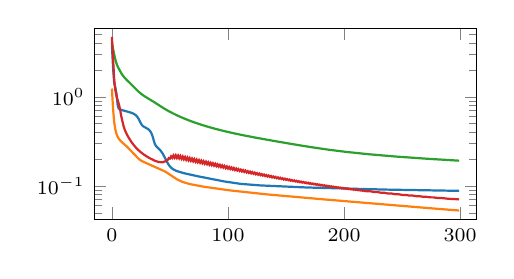
\begin{tikzpicture}

\definecolor{crimson2143940}{RGB}{214,39,40}
\definecolor{darkgray176}{RGB}{176,176,176}
\definecolor{darkorange25512714}{RGB}{255,127,14}
\definecolor{forestgreen4416044}{RGB}{44,160,44}
\definecolor{steelblue31119180}{RGB}{31,119,180}

\begin{axis}[compar,
	ymode=log]
\addplot [thick, steelblue31119180]
table {%
0 3.85001611709595
1 2.1458203792572
2 1.42304074764252
3 1.27057814598083
4 1.07568347454071
5 0.799212455749512
6 0.733221530914307
7 0.721283674240112
9 0.707787752151489
16 0.666974186897278
18 0.651615381240845
19 0.64179801940918
20 0.629560708999634
21 0.613784790039062
22 0.593032360076904
23 0.566002249717712
25 0.501725912094116
26 0.47937273979187
27 0.46651017665863
29 0.451001048088074
31 0.43555474281311
32 0.425134420394897
33 0.41105580329895
34 0.391023635864258
35 0.362361192703247
36 0.326099514961243
37 0.295191526412964
38 0.280576586723328
42 0.248737454414368
44 0.227878451347351
48 0.180903553962708
49 0.172060966491699
51 0.160104870796204
53 0.153125762939453
56 0.146742224693298
62 0.13903284072876
74 0.128426432609558
97 0.112231850624084
111 0.105488300323486
128 0.101377844810486
168 0.0961171388626099
235 0.0910736322402954
299 0.0881310701370239
};
\addplot [thick, darkorange25512714]
table {%
0 1.23822641372681
1 0.738285541534424
2 0.515761375427246
3 0.4292893409729
4 0.38191545009613
5 0.354934692382812
6 0.338408708572388
7 0.325846433639526
9 0.306785702705383
13 0.275501608848572
23 0.201859831809998
25 0.192705988883972
28 0.184560060501099
46 0.144832253456116
56 0.118885040283203
61 0.110710263252258
67 0.105042099952698
79 0.0981142520904541
101 0.0893926620483398
133 0.0805541276931763
184 0.0704268217086792
280 0.0554471015930176
299 0.0530545711517334
};
\addplot [thick, forestgreen4416044]
table {%
0 4.05598926544189
1 3.45300483703613
2 2.97763061523438
3 2.61971783638
4 2.35778474807739
5 2.18703508377075
6 2.06520247459412
7 1.95468974113464
8 1.84842002391815
9 1.76255404949188
10 1.69462144374847
11 1.63581776618958
12 1.58327627182007
13 1.53526997566223
14 1.49058413505554
16 1.40748488903046
21 1.20854544639587
22 1.17382073402405
23 1.14177072048187
24 1.11227011680603
25 1.08525025844574
26 1.06055045127869
28 1.01695835590363
30 0.978874087333679
33 0.927088260650635
37 0.862118482589722
44 0.752540469169617
46 0.725320339202881
49 0.689407587051392
52 0.657606840133667
55 0.628973245620728
59 0.595095992088318
63 0.565508365631104
67 0.539439916610718
72 0.510800004005432
77 0.485812664031982
83 0.459864139556885
89 0.437418222427368
96 0.414665579795837
104 0.392243146896362
113 0.370553493499756
124 0.347705125808716
138 0.322409272193909
155 0.295305252075195
171 0.273048043251038
186 0.255640983581543
202 0.240770101547241
221 0.226953506469727
244 0.213955640792847
273 0.201248288154602
299 0.192145466804504
};
\addplot [thick, crimson2143940]
table {%
0 4.69362020492554
1 2.7148494720459
2 1.54917848110199
3 1.17751252651215
4 1.0149405002594
5 0.90976893901825
6 0.828250408172607
7 0.726314544677734
8 0.61180305480957
9 0.536312222480774
10 0.472319364547729
11 0.429957985877991
12 0.400319814682007
13 0.376694202423096
14 0.356591105461121
15 0.338947892189026
17 0.309252738952637
19 0.285506248474121
21 0.266453266143799
23 0.251017570495605
26 0.232697129249573
29 0.218315958976746
33 0.203232884407043
37 0.191822648048401
40 0.185920238494873
43 0.184518098831177
44 0.184627890586853
45 0.187541604042053
46 0.188506722450256
47 0.194794178009033
48 0.195274114608765
49 0.205084681510925
50 0.202417969703674
51 0.214552879333496
52 0.206847906112671
53 0.219677567481995
54 0.207814335823059
55 0.220445871353149
56 0.206572294235229
57 0.218820691108704
58 0.204374670982361
59 0.216279745101929
60 0.201866745948792
61 0.213473916053772
62 0.199298739433289
63 0.210629820823669
64 0.196754813194275
65 0.207815408706665
66 0.194255113601685
67 0.205044865608215
68 0.191802024841309
69 0.202317833900452
70 0.189392685890198
71 0.199632048606873
72 0.187022805213928
73 0.196983456611633
74 0.184688091278076
75 0.194367408752441
76 0.182385087013245
77 0.191782355308533
78 0.180112361907959
79 0.189228415489197
80 0.177868366241455
81 0.186703562736511
82 0.175650596618652
83 0.184206366539001
84 0.173459053039551
85 0.181738138198853
86 0.171293258666992
87 0.179298281669617
88 0.169152617454529
89 0.176887392997742
90 0.167037963867188
91 0.174506902694702
92 0.16494882106781
93 0.172156095504761
94 0.162885546684265
95 0.169836640357971
96 0.160848617553711
97 0.167548418045044
98 0.158838629722595
99 0.165292978286743
100 0.156855821609497
101 0.163070917129517
102 0.154901623725891
103 0.160883188247681
104 0.15297532081604
105 0.158729791641235
106 0.15107786655426
107 0.156611561775208
108 0.149209976196289
109 0.154529452323914
110 0.147372007369995
111 0.152483701705933
112 0.145563960075378
113 0.150474071502686
114 0.143786668777466
115 0.148502349853516
116 0.142040610313416
117 0.146567940711975
118 0.140325665473938
119 0.144671440124512
120 0.138642072677612
121 0.14281153678894
122 0.136988997459412
123 0.140989542007446
124 0.135367751121521
125 0.139204740524292
126 0.133777260780334
127 0.137457251548767
128 0.132217884063721
129 0.135746121406555
130 0.130689024925232
131 0.134072184562683
132 0.129191517829895
133 0.132434606552124
134 0.127724409103394
135 0.130833268165588
136 0.126287460327148
137 0.129267334938049
138 0.124881029129028
139 0.127737283706665
140 0.123503923416138
141 0.126241326332092
142 0.122155427932739
143 0.124778866767883
144 0.120835781097412
145 0.123349666595459
146 0.11954402923584
147 0.12195360660553
148 0.118280410766602
149 0.120589852333069
150 0.117044448852539
151 0.119257688522339
152 0.115834832191467
153 0.117956519126892
154 0.114651560783386
155 0.116685271263123
156 0.113493919372559
157 0.115443706512451
158 0.112361907958984
159 0.11423134803772
160 0.111255049705505
161 0.113047957420349
162 0.110172152519226
163 0.111891508102417
164 0.109112620353699
165 0.110761642456055
166 0.108076214790344
167 0.109657764434814
168 0.107062339782715
169 0.108580470085144
170 0.106070995330811
171 0.107527494430542
172 0.105100989341736
173 0.106499433517456
174 0.10415244102478
175 0.105494618415833
176 0.103224039077759
177 0.104513049125671
178 0.102315545082092
179 0.103553533554077
180 0.101426720619202
181 0.102616190910339
182 0.100557088851929
183 0.101700305938721
184 0.0997061729431152
185 0.100804686546326
186 0.0988726615905762
187 0.0999287366867065
188 0.0980567932128906
189 0.0990729331970215
190 0.0972588062286377
191 0.0982364416122437
192 0.0964773893356323
193 0.097417950630188
194 0.0957117080688477
195 0.0966169834136963
196 0.0949617624282837
197 0.0958337783813477
198 0.0942277908325195
199 0.0950677394866943
200 0.0935087203979492
201 0.0943180322647095
202 0.0928041934967041
203 0.093584418296814
204 0.0921140909194946
205 0.0928663015365601
206 0.0914373397827148
207 0.0921628475189209
208 0.0907740592956543
209 0.091474175453186
210 0.0901238918304443
211 0.0907998085021973
212 0.089486837387085
213 0.090139627456665
214 0.0888618230819702
215 0.0894925594329834
216 0.0882493257522583
217 0.088858962059021
218 0.0876481533050537
220 0.0870583057403564
223 0.0870314836502075
226 0.085355281829834
229 0.0853092670440674
232 0.0837435722351074
235 0.0836825370788574
238 0.0822173357009888
241 0.082144021987915
244 0.0807691812515259
247 0.0806872844696045
250 0.0793938636779785
253 0.0793051719665527
256 0.0780863761901855
259 0.0779929161071777
262 0.0768417119979858
265 0.0767456293106079
268 0.0756555795669556
271 0.0755575895309448
274 0.0745236873626709
277 0.0744255781173706
280 0.0734424591064453
285 0.072994589805603
290 0.0717432498931885
295 0.0713222026824951
299 0.0706861019134521
};
\end{axis}

\end{tikzpicture}
}
	&
	\multicolumn{4}{c}{% This file was created with tikzplotlib v0.10.1.
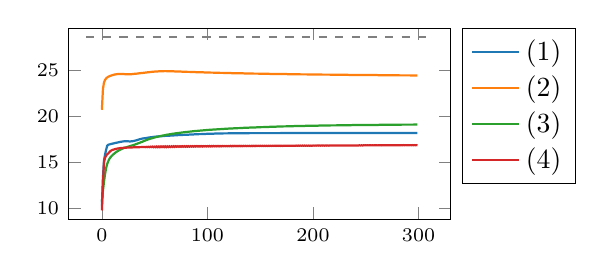
\begin{tikzpicture}

\definecolor{crimson2143940}{RGB}{214,39,40}
\definecolor{darkgray176}{RGB}{176,176,176}
\definecolor{darkorange25512714}{RGB}{255,127,14}
\definecolor{forestgreen4416044}{RGB}{44,160,44}
\definecolor{steelblue31119180}{RGB}{31,119,180}

\begin{axis}[compar, legend pos=outer north east]
\addplot [thick, steelblue31119180]
table {%
0 10.3199996948242
1 13.3599996566772
2 15.210000038147
3 15.8400001525879
4 16.3500003814697
5 16.7999992370605
6 16.8999996185303
7 16.9400005340576
10 17.0300006866455
11 17.0499992370605
13 17.1100006103516
14 17.1299991607666
15 17.1599998474121
16 17.1800003051758
17 17.2099990844727
20 17.2700004577637
22 17.2900009155273
24 17.2900009155273
26 17.2700004577637
27 17.2700004577637
29 17.2900009155273
30 17.3199996948242
31 17.3400001525879
33 17.3999996185303
35 17.4799995422363
38 17.5699996948242
40 17.6100006103516
41 17.6200008392334
46 17.7199993133545
47 17.7299995422363
48 17.75
49 17.7600002288818
50 17.7800006866455
56 17.8400001525879
57 17.8400001525879
60 17.8700008392334
61 17.8700008392334
63 17.8899993896484
64 17.8899993896484
66 17.9099998474121
67 17.9099998474121
69 17.9300003051758
70 17.9300003051758
72 17.9500007629395
73 17.9500007629395
74 17.9599990844727
75 17.9599990844727
77 17.9799995422363
78 17.9799995422363
79 17.9899997711182
80 17.9899997711182
81 18
82 18
83 18.0100002288818
84 18.0100002288818
86 18.0300006866455
87 18.0300006866455
88 18.0400009155273
89 18.0400009155273
90 18.0499992370605
91 18.0499992370605
92 18.0599994659424
94 18.0599994659424
95 18.0699996948242
96 18.0699996948242
97 18.0799999237061
98 18.0799999237061
99 18.0900001525879
101 18.0900001525879
102 18.1000003814697
103 18.1000003814697
104 18.1100006103516
106 18.1100006103516
107 18.1200008392334
110 18.1200008392334
111 18.1299991607666
114 18.1299991607666
115 18.1399993896484
119 18.1399993896484
120 18.1499996185303
126 18.1499996185303
127 18.1599998474121
139 18.1599998474121
140 18.1700000762939
169 18.1700000762939
170 18.1800003051758
241 18.1800003051758
242 18.1900005340576
299 18.1900005340576
};
\addlegendentry{$(1)$}
\addplot [thick, darkorange25512714]
table {%
0 20.7000007629395
1 22.9500007629395
2 23.6599998474121
3 23.9300003051758
4 24.1000003814697
5 24.2000007629395
6 24.2800006866455
8 24.3799991607666
10 24.4599990844727
12 24.5200004577637
14 24.5599994659424
16 24.5799999237061
17 24.5799999237061
18 24.5900001525879
19 24.5799999237061
20 24.5799999237061
22 24.5599994659424
23 24.5599994659424
24 24.5499992370605
27 24.5499992370605
30 24.5799999237061
31 24.6000003814697
34 24.6299991607666
35 24.6499996185303
36 24.6599998474121
37 24.6800003051758
39 24.7000007629395
40 24.7199993133545
42 24.7399997711182
43 24.7600002288818
45 24.7800006866455
46 24.7999992370605
52 24.8600006103516
53 24.8600006103516
55 24.8799991607666
58 24.8799991607666
59 24.8899993896484
61 24.8899993896484
62 24.8799991607666
65 24.8799991607666
66 24.8700008392334
68 24.8700008392334
69 24.8600006103516
71 24.8600006103516
72 24.8500003814697
73 24.8500003814697
74 24.8400001525879
75 24.8400001525879
76 24.8299999237061
78 24.8299999237061
79 24.8199996948242
80 24.8199996948242
81 24.8099994659424
83 24.8099994659424
84 24.7999992370605
85 24.7999992370605
86 24.7900009155273
88 24.7900009155273
89 24.7800006866455
90 24.7800006866455
91 24.7700004577637
93 24.7700004577637
94 24.7600002288818
96 24.7600002288818
97 24.75
99 24.75
100 24.7399997711182
102 24.7399997711182
103 24.7299995422363
105 24.7299995422363
106 24.7199993133545
108 24.7199993133545
109 24.7099990844727
111 24.7099990844727
112 24.7000007629395
115 24.7000007629395
116 24.6900005340576
119 24.6900005340576
120 24.6800003051758
122 24.6800003051758
123 24.6700000762939
126 24.6700000762939
127 24.6599998474121
130 24.6599998474121
131 24.6499996185303
134 24.6499996185303
135 24.6399993896484
139 24.6399993896484
140 24.6299991607666
143 24.6299991607666
144 24.6200008392334
148 24.6200008392334
149 24.6100006103516
153 24.6100006103516
154 24.6000003814697
158 24.6000003814697
159 24.5900001525879
163 24.5900001525879
164 24.5799999237061
169 24.5799999237061
170 24.5699996948242
175 24.5699996948242
176 24.5599994659424
181 24.5599994659424
182 24.5499992370605
187 24.5499992370605
188 24.5400009155273
194 24.5400009155273
195 24.5300006866455
201 24.5300006866455
202 24.5200004577637
208 24.5200004577637
209 24.5100002288818
216 24.5100002288818
217 24.5
224 24.5
225 24.4899997711182
233 24.4899997711182
234 24.4799995422363
241 24.4799995422363
242 24.4699993133545
251 24.4699993133545
252 24.4599990844727
261 24.4599990844727
262 24.4500007629395
271 24.4500007629395
272 24.4400005340576
281 24.4400005340576
282 24.4300003051758
292 24.4300003051758
293 24.4200000762939
299 24.4200000762939
};
\addlegendentry{$(2)$}
\addplot [thick, forestgreen4416044]
table {%
0 10.7299995422363
1 11.8900003433228
2 12.9099998474121
3 13.7200002670288
4 14.3699998855591
5 14.8100004196167
6 15.1099996566772
7 15.3500003814697
8 15.5299997329712
9 15.6599998474121
10 15.7799997329712
12 15.9799995422363
13 16.0699996948242
14 16.1499996185303
16 16.2900009155273
18 16.4099998474121
21 16.5599994659424
22 16.6000003814697
23 16.6299991607666
24 16.6700000762939
25 16.7000007629395
26 16.7399997711182
27 16.7700004577637
28 16.8099994659424
29 16.8400001525879
33 17
34 17.0499992370605
36 17.1299991607666
37 17.1800003051758
38 17.2199993133545
40 17.3199996948242
41 17.3600006103516
42 17.4099998474121
46 17.5699996948242
48 17.6299991607666
49 17.6700000762939
51 17.7299995422363
52 17.75
55 17.8400001525879
56 17.8600006103516
57 17.8899993896484
59 17.9300003051758
60 17.9599990844727
67 18.1000003814697
68 18.1100006103516
70 18.1499996185303
71 18.1599998474121
72 18.1800003051758
73 18.1900005340576
74 18.2099990844727
75 18.2199993133545
76 18.2399997711182
77 18.25
78 18.2700004577637
81 18.2999992370605
82 18.3199996948242
85 18.3500003814697
86 18.3700008392334
102 18.5300006866455
103 18.5300006866455
107 18.5699996948242
108 18.5699996948242
111 18.6000003814697
112 18.6000003814697
114 18.6200008392334
115 18.6200008392334
117 18.6399993896484
118 18.6399993896484
120 18.6599998474121
121 18.6599998474121
122 18.6700000762939
123 18.6700000762939
125 18.6900005340576
126 18.6900005340576
127 18.7000007629395
128 18.7000007629395
129 18.7099990844727
130 18.7099990844727
131 18.7199993133545
132 18.7199993133545
134 18.7399997711182
135 18.7399997711182
136 18.75
137 18.75
138 18.7600002288818
139 18.7600002288818
140 18.7700004577637
142 18.7700004577637
143 18.7800006866455
144 18.7800006866455
145 18.7900009155273
146 18.7900009155273
147 18.7999992370605
148 18.7999992370605
149 18.8099994659424
150 18.8099994659424
151 18.8199996948242
153 18.8199996948242
154 18.8299999237061
155 18.8299999237061
156 18.8400001525879
158 18.8400001525879
159 18.8500003814697
160 18.8500003814697
161 18.8600006103516
163 18.8600006103516
164 18.8700008392334
165 18.8700008392334
166 18.8799991607666
168 18.8799991607666
169 18.8899993896484
171 18.8899993896484
172 18.8999996185303
174 18.8999996185303
175 18.9099998474121
177 18.9099998474121
178 18.9200000762939
181 18.9200000762939
182 18.9300003051758
184 18.9300003051758
185 18.9400005340576
188 18.9400005340576
189 18.9500007629395
192 18.9500007629395
193 18.9599990844727
196 18.9599990844727
197 18.9699993133545
201 18.9699993133545
202 18.9799995422363
205 18.9799995422363
206 18.9899997711182
211 18.9899997711182
212 19
216 19
217 19.0100002288818
222 19.0100002288818
223 19.0200004577637
229 19.0200004577637
230 19.0300006866455
236 19.0300006866455
237 19.0400009155273
244 19.0400009155273
245 19.0499992370605
253 19.0499992370605
254 19.0599994659424
262 19.0599994659424
263 19.0699996948242
272 19.0699996948242
273 19.0799999237061
283 19.0799999237061
284 19.0900001525879
295 19.0900001525879
296 19.1000003814697
299 19.1000003814697
};
\addlegendentry{$(3)$}
\addplot [thick, crimson2143940]
table {%
0 9.77999973297119
1 12.6499996185303
2 15.0299997329712
3 15.4799995422363
4 15.7200002670288
5 15.8699998855591
6 15.9700002670288
8 16.2099990844727
9 16.2900009155273
10 16.3500003814697
11 16.3799991607666
12 16.4200000762939
14 16.4799995422363
16 16.5200004577637
17 16.5300006866455
18 16.5499992370605
22 16.5900001525879
23 16.5900001525879
24 16.6000003814697
25 16.6000003814697
26 16.6100006103516
27 16.6100006103516
28 16.6200008392334
29 16.6200008392334
30 16.6299991607666
31 16.6299991607666
32 16.6399993896484
33 16.6399993896484
34 16.6499996185303
35 16.6399993896484
36 16.6499996185303
37 16.6499996185303
38 16.6599998474121
39 16.6499996185303
40 16.6700000762939
41 16.6499996185303
42 16.6800003051758
43 16.6499996185303
44 16.6900005340576
45 16.6499996185303
46 16.7000007629395
47 16.6499996185303
48 16.7099990844727
49 16.6399993896484
50 16.7099990844727
51 16.6399993896484
52 16.7199993133545
53 16.6399993896484
54 16.7199993133545
55 16.6399993896484
56 16.7299995422363
57 16.6499996185303
58 16.7299995422363
59 16.6499996185303
60 16.7399997711182
61 16.6499996185303
62 16.7399997711182
63 16.6599998474121
64 16.7399997711182
65 16.6599998474121
66 16.7399997711182
67 16.6700000762939
68 16.75
69 16.6700000762939
70 16.75
71 16.6800003051758
72 16.75
73 16.6800003051758
74 16.75
75 16.6800003051758
76 16.7600002288818
77 16.6900005340576
78 16.7600002288818
79 16.6900005340576
80 16.7600002288818
81 16.6900005340576
82 16.7600002288818
83 16.7000007629395
84 16.7600002288818
85 16.7000007629395
86 16.7600002288818
87 16.7000007629395
88 16.7700004577637
89 16.7099990844727
90 16.7700004577637
91 16.7099990844727
92 16.7700004577637
93 16.7099990844727
94 16.7700004577637
95 16.7099990844727
96 16.7700004577637
97 16.7199993133545
98 16.7700004577637
99 16.7199993133545
100 16.7700004577637
101 16.7199993133545
102 16.7800006866455
103 16.7199993133545
104 16.7800006866455
105 16.7299995422363
106 16.7800006866455
107 16.7299995422363
108 16.7800006866455
109 16.7299995422363
110 16.7800006866455
111 16.7299995422363
112 16.7800006866455
113 16.7299995422363
114 16.7800006866455
115 16.7399997711182
116 16.7800006866455
117 16.7399997711182
118 16.7800006866455
119 16.7399997711182
120 16.7800006866455
121 16.7399997711182
122 16.7900009155273
123 16.7399997711182
124 16.7900009155273
125 16.75
126 16.7900009155273
127 16.75
128 16.7900009155273
129 16.75
130 16.7900009155273
131 16.75
132 16.7900009155273
133 16.75
134 16.7900009155273
135 16.7600002288818
136 16.7900009155273
137 16.7600002288818
138 16.7900009155273
139 16.7600002288818
140 16.7900009155273
141 16.7600002288818
142 16.7999992370605
143 16.7600002288818
144 16.7999992370605
145 16.7600002288818
146 16.7999992370605
147 16.7700004577637
148 16.7999992370605
149 16.7700004577637
150 16.7999992370605
151 16.7700004577637
152 16.7999992370605
153 16.7700004577637
154 16.7999992370605
155 16.7700004577637
156 16.7999992370605
157 16.7700004577637
158 16.7999992370605
159 16.7800006866455
160 16.7999992370605
161 16.7800006866455
162 16.7999992370605
163 16.7800006866455
164 16.8099994659424
165 16.7800006866455
166 16.8099994659424
167 16.7800006866455
168 16.8099994659424
169 16.7800006866455
170 16.8099994659424
171 16.7800006866455
172 16.8099994659424
173 16.7900009155273
174 16.8099994659424
175 16.7900009155273
176 16.8099994659424
177 16.7900009155273
178 16.8099994659424
179 16.7900009155273
180 16.8099994659424
181 16.7900009155273
182 16.8099994659424
183 16.7900009155273
184 16.8199996948242
185 16.7900009155273
186 16.8199996948242
187 16.7999992370605
188 16.8199996948242
189 16.7999992370605
190 16.8199996948242
191 16.7999992370605
192 16.8199996948242
193 16.7999992370605
194 16.8199996948242
195 16.7999992370605
196 16.8199996948242
197 16.7999992370605
198 16.8199996948242
199 16.7999992370605
200 16.8199996948242
201 16.8099994659424
202 16.8199996948242
203 16.8099994659424
204 16.8299999237061
205 16.8099994659424
206 16.8299999237061
207 16.8099994659424
208 16.8299999237061
209 16.8099994659424
210 16.8299999237061
211 16.8099994659424
212 16.8299999237061
213 16.8099994659424
214 16.8299999237061
215 16.8099994659424
216 16.8299999237061
217 16.8199996948242
218 16.8299999237061
219 16.8199996948242
220 16.8299999237061
221 16.8199996948242
222 16.8299999237061
223 16.8199996948242
224 16.8400001525879
225 16.8199996948242
226 16.8400001525879
227 16.8199996948242
228 16.8400001525879
229 16.8199996948242
230 16.8400001525879
231 16.8199996948242
232 16.8400001525879
233 16.8299999237061
234 16.8400001525879
235 16.8299999237061
236 16.8400001525879
237 16.8299999237061
238 16.8400001525879
239 16.8299999237061
240 16.8400001525879
241 16.8299999237061
242 16.8400001525879
243 16.8299999237061
244 16.8500003814697
245 16.8299999237061
246 16.8500003814697
247 16.8299999237061
248 16.8500003814697
249 16.8400001525879
250 16.8500003814697
251 16.8400001525879
252 16.8500003814697
253 16.8400001525879
254 16.8500003814697
255 16.8400001525879
256 16.8500003814697
257 16.8400001525879
258 16.8500003814697
259 16.8400001525879
260 16.8500003814697
261 16.8400001525879
262 16.8500003814697
263 16.8400001525879
264 16.8600006103516
265 16.8400001525879
266 16.8600006103516
267 16.8500003814697
268 16.8600006103516
269 16.8500003814697
270 16.8600006103516
271 16.8500003814697
272 16.8600006103516
273 16.8500003814697
274 16.8600006103516
275 16.8500003814697
276 16.8600006103516
277 16.8500003814697
278 16.8600006103516
279 16.8500003814697
280 16.8600006103516
281 16.8500003814697
282 16.8600006103516
283 16.8500003814697
284 16.8700008392334
285 16.8600006103516
286 16.8700008392334
287 16.8600006103516
288 16.8700008392334
289 16.8600006103516
290 16.8700008392334
291 16.8600006103516
292 16.8700008392334
293 16.8600006103516
294 16.8700008392334
295 16.8600006103516
296 16.8700008392334
297 16.8600006103516
298 16.8700008392334
299 16.8600006103516
};
\addlegendentry{$(4)$}
\addplot [thick, gray, dashed]
table {%
-14.95 28.6013965606689
313.95 28.6013965606689
};
\end{axis}

\end{tikzpicture}
}
\end{tabular}
	\caption{$d=800$, sans passe-base}
	\label{fig:LGDlat800-s}
\end{figure}

\begin{figure}[H]\centering
	\begin{tabular}{c c c c c c}
	Target  &  $(1)$  &  $(2)$  &  $(3)$   &  $(4)$
	
	\\
	
	\multirow{2}{0.3\textwidth}[0.122\textwidth]{\includegraphics[width=0.3\textwidth]{resultats/LGD/lats/lat-800-target-g.png}}
	&
	\includegraphics[width=0.15\textwidth]{resultats/LGD/lats/lat-800_1-init-pas=10.0_filtre=g-0.6.png}
	&
	\includegraphics[width=0.15\textwidth]{resultats/LGD/lats/lat-800_2-init-pas=10.0_filtre=g-0.6.png}
	&
	\includegraphics[width=0.15\textwidth]{resultats/LGD/lats/lat-800_3-init-pas=10.0_filtre=g-0.6.png}
	&
	\includegraphics[width=0.15\textwidth]{resultats/LGD/lats/lat-800_4-init-pas=10.0_filtre=g-0.6.png}
	
	\\
	
	
	&
	\includegraphics[width=0.15\textwidth]{resultats/LGD/lats/lat-800_1-guess-pas=10.0_filtre=g-0.6.png}
	&
	\includegraphics[width=0.15\textwidth]{resultats/LGD/lats/lat-800_2-guess-pas=10.0_filtre=g-0.6.png}
	&
	\includegraphics[width=0.15\textwidth]{resultats/LGD/lats/lat-800_3-guess-pas=10.0_filtre=g-0.6.png}
	&
	\includegraphics[width=0.15\textwidth]{resultats/LGD/lats/lat-800_4-guess-pas=10.0_filtre=g-0.6.png}
	
	\\ \\
	
	
	
	\multicolumn{2}{c}{Loss}  &  \multicolumn{4}{c}{PSNR{\color{white}bbbb}}
	
	\\
	
	\multicolumn{2}{c}{% This file was created with tikzplotlib v0.10.1.
\begin{tikzpicture}

\definecolor{crimson2143940}{RGB}{214,39,40}
\definecolor{darkgray176}{RGB}{176,176,176}
\definecolor{darkorange25512714}{RGB}{255,127,14}
\definecolor{forestgreen4416044}{RGB}{44,160,44}
\definecolor{steelblue31119180}{RGB}{31,119,180}

\begin{axis}[
height=\figheight,
tick align=outside,
tick pos=left,
width=\figwidth,
x grid style={darkgray176},
xmin=-0.95, xmax=19.95,
xtick style={color=black},
y grid style={darkgray176},
ymin=-0.547165866941214, ymax=15.0585420243442,
ytick style={color=black}
]
\addplot [semithick, steelblue31119180]
table {%
0 2.93553948402405
1 1.87434804439545
2 1.10162699222565
3 0.695515155792236
4 0.369987845420837
5 0.243139982223511
6 0.179080009460449
8 0.162184476852417
15 0.184467554092407
19 0.200243592262268
};
\addplot [semithick, darkorange25512714]
table {%
0 1.26624810695648
1 0.418554663658142
2 0.244757056236267
3 0.188532590866089
4 0.177584409713745
5 0.173996567726135
10 0.190012454986572
16 0.208758592605591
19 0.212993383407593
};
\addplot [semithick, forestgreen4416044]
table {%
0 14.3491916656494
1 3.53692412376404
2 2.17629098892212
3 1.30119788646698
4 0.828463077545166
5 0.442574858665466
6 0.278957962989807
7 0.191884636878967
8 0.172186493873596
9 0.162286520004272
15 0.176749229431152
19 0.193746089935303
};
\addplot [semithick, crimson2143940]
table {%
0 6.1989574432373
1 2.70222043991089
2 1.7502475976944
3 1.00837326049805
4 0.632613182067871
5 0.344910740852356
6 0.230880498886108
7 0.176201343536377
9 0.163307666778564
19 0.198582410812378
};
\end{axis}

\end{tikzpicture}
}
	&
	\multicolumn{4}{c}{% This file was created with tikzplotlib v0.10.1.
\begin{tikzpicture}

\definecolor{crimson2143940}{RGB}{214,39,40}
\definecolor{darkgray176}{RGB}{176,176,176}
\definecolor{darkorange25512714}{RGB}{255,127,14}
\definecolor{forestgreen4416044}{RGB}{44,160,44}
\definecolor{steelblue31119180}{RGB}{31,119,180}

\begin{axis}[
height=\figheight,
tick align=outside,
tick pos=left,
width=\figwidth,
x grid style={darkgray176},
xmin=-0.95, xmax=19.95,
xtick style={color=black},
y grid style={darkgray176},
ymin=-2.57960711717606, ymax=31.5117500901222,
ytick style={color=black}
]
\addplot [semithick, steelblue31119180]
table {%
0 11.3299999237061
1 14.5600004196167
2 18.4799995422363
3 21.3500003814697
4 24.9899997711182
5 26.6900005340576
6 27.5400009155273
7 27.7600002288818
8 27.8400001525879
9 27.8199996948242
10 27.7700004577637
11 27.6599998474121
12 27.5100002288818
13 27.3199996948242
16 26.6900005340576
17 26.5
18 26.3199996948242
19 26.1700000762939
};
\addplot [semithick, darkorange25512714]
table {%
0 10.9399995803833
1 22.8500003814697
2 25.7900009155273
3 27.0400009155273
4 27.4300003051758
5 27.5200004577637
6 27.4400005340576
7 27.3099994659424
8 27.1399993896484
9 26.9500007629395
11 26.5499992370605
12 26.3700008392334
13 26.2099990844727
14 26.0599994659424
15 25.9400005340576
16 25.8400001525879
17 25.7600002288818
18 25.6900005340576
19 25.6299991607666
};
\addplot [semithick, forestgreen4416044]
table {%
0 -1.02999997138977
1 10.1499996185303
2 13.5299997329712
3 17.3600006103516
4 20.2299995422363
5 24.0400009155273
6 26.1100006103516
7 27.2600002288818
8 27.6299991607666
9 27.75
10 27.7800006866455
11 27.7700004577637
12 27.7000007629395
13 27.5799999237061
14 27.4200000762939
15 27.2299995422363
18 26.6299991607666
19 26.4500007629395
};
\addplot [semithick, crimson2143940]
table {%
0 5.21000003814697
1 12.0100002288818
2 15.1099996566772
3 19.0200004577637
4 21.9400005340576
5 25.2000007629395
6 26.8199996948242
7 27.5
8 27.6599998474121
9 27.6900005340576
10 27.6200008392334
11 27.5300006866455
12 27.3899993896484
13 27.2299995422363
14 27.0499992370605
15 26.8600006103516
16 26.6800003051758
17 26.5100002288818
18 26.3500003814697
19 26.2000007629395
};
\addplot [semithick, gray]
table {%
-0.95 29.9621429443359
19.95 29.9621429443359
};
\end{axis}

\end{tikzpicture}
}
\end{tabular}
	\caption{$d=800$, avec passe-base gaussien ($\sigma=0.6$)}
	\label{fig:LGDlat800-g}
\end{figure}





\newpage



\subsection{Comparaison avec la descente de gradient projetée}\label{sec:PGD}
\quad

La descente de gradient projeté (PGD) par auto-encodeur, comme son nom l'indique, consiste en une descente de gradient classique à cela près qu'à chaque itération, le vecteur obtenu est projeté par une fonction$p$ (voir \figref{fig:pcode PGD} ci-contre).

\begin{wrapfigure}{r}{0.44\textwidth}
	\fbox{\begin{minipage}{18em}
\vspace{0.3cm}
\begin{algorithmic}[0]
    \State $x_0$ : initialisation
    \State $x$ : image à reconstruire
    \State $\rho$ : pas de descente
    \State $N$ : nombre d'itération
    \State $y\ \ll\ A(x)$
    \State
    \For{$n\in \llbracket1,N-1\rrbracket$}
        \State $\nabla F(x_n)\ \ll\ ^tA\big(Ax_n-y_0\big)$
        \State $\ \ x_{n+1}\quad  \ll\ p\big(x_n\ - \rho \nabla F(x_n)\big)$
        \EndFor
    \State
    \Return $(x_n)_{0\leq n\leq N}$
\end{algorithmic}
\vspace{0.2cm}
\end{minipage}}
	\caption{Algorithme de PGD}
	\label{fig:pcode PGD}
\end{wrapfigure}
\noindent Ce rapport étant surtout porté sur la descente de gradient depuis l'espace latent de $p$, on ne détaillera pas les arguments mathématiques qui supportent cette méthode mais on peut tout de même essayer de se convaincre de l'intérêt de la PGD.\\
Comme expliqué plus haut, le problème est convexe ce qui assure la convergence de la descente de gradient. La difficulté étant de tomber sur un ``bon'' argmin. C'est là que composer par $p$ peut aider à diriger la descente vers le bon minimum. Si on parle de descente \emph{projetée} c'est aussi parce que, en appliquant $p$, on s'assure qu'à chaque itération l'image en reconstruction $\bf{x}_n$ appartient au modèle de basse dimension $\Sigma$.

Là encore, il n’y a pas de définition claire pour $\Sigma$ pour les images et donc pas de moyen de construire simplement une projection. C’est là qu’un intervient le réseau $f$.
L'auto-encodeur étant entraîné sur les données, $f$ doit pouvoir faire office de projection pour des images qui ne sont pas trop éloignées de $\Sigma$. Cette méthode est tirée de l'article \cite{peng_solving_2019} de P. Peng, S. Jalali and X. Yuan et on a pu reproduire leurs résultats. 
\\

Comme précédemment, dans les figures \textit{\ref{fig:PGDbackproj-s}} à \textit{\ref{fig:PGDgauss-g}}, plusieurs PGD sont effectuées, un coup sans filtre passe-bas, un coup avec. Les deux premières sont initialisées par backprojeciton (\ei par $^tA\bf{y_0}$), les deux suivantes par des vecteurs aléatoires tirés suivant une loi uniforme sur $[0,1]$ et les deux dernières suivant une loi normale d'écart-type 2.
\\
Dans tous les cas, il est clair que la descente projetée est moins efficace que la LGD. Par contre, elle converge beaucoup plus vite : en seulement une quinzaine d’itérations la loss ne descend plus mais commence à remonter. Cette remontée est très probablement dû au fait que le gradient est devenu quasiment nul et que l’algorithme revient à appliquer $f$ en boucle. Comme l'auto-encodeur c’est pas équivalent à l’application identité, on constate une dérive.
\\
De plus, si la PGD est moins efficace que la LGD, les figures \textit{\ref{fig:PGDgauss-s}} et \textit{\ref{fig:PGDgauss-g}} montre qu’elle est en revanche plus robuste à l’initialisation par des vecteurs en dehors de $[0,1]^{n\times m}$.
\\

\begin{figure}[H]\centering
	\begin{tabular}{c c c c c c c c c}
$(1)$  &  $(2)$  &  $(3)$  &  $(4)$  &  $(5)$  &  $(6)$  &  $(7)$  &  $(8)$

\\

\includegraphics[width=0.1\textwidth]{resultats/PGD/multitarget/backproj_1-init-pas=1.25_filtre=s-None}
&
\includegraphics[width=0.1\textwidth]{resultats/PGD/multitarget/backproj_2-init-pas=1.25_filtre=s-None}
&
\includegraphics[width=0.1\textwidth]{resultats/PGD/multitarget/backproj_3-init-pas=1.25_filtre=s-None}
&
\includegraphics[width=0.1\textwidth]{resultats/PGD/multitarget/backproj_4-init-pas=1.25_filtre=s-None}
&
\includegraphics[width=0.1\textwidth]{resultats/PGD/multitarget/backproj_5-init-pas=1.25_filtre=s-None}
&
\includegraphics[width=0.1\textwidth]{resultats/PGD/multitarget/backproj_6-init-pas=1.25_filtre=s-None}
&
\includegraphics[width=0.1\textwidth]{resultats/PGD/multitarget/backproj_7-init-pas=1.25_filtre=s-None}
&
\includegraphics[width=0.1\textwidth]{resultats/PGD/multitarget/backproj_8-init-pas=1.25_filtre=s-None}

\\

\includegraphics[width=0.1\textwidth]{resultats/PGD/multitarget/backproj_1-guess-pas=1.25_filtre=s-None}
&
\includegraphics[width=0.1\textwidth]{resultats/PGD/multitarget/backproj_2-guess-pas=1.25_filtre=s-None}
&
\includegraphics[width=0.1\textwidth]{resultats/PGD/multitarget/backproj_3-guess-pas=1.25_filtre=s-None}
&
\includegraphics[width=0.1\textwidth]{resultats/PGD/multitarget/backproj_4-guess-pas=1.25_filtre=s-None}
&
\includegraphics[width=0.1\textwidth]{resultats/PGD/multitarget/backproj_5-guess-pas=1.25_filtre=s-None}
&
\includegraphics[width=0.1\textwidth]{resultats/PGD/multitarget/backproj_6-guess-pas=1.25_filtre=s-None}
&
\includegraphics[width=0.1\textwidth]{resultats/PGD/multitarget/backproj_7-guess-pas=1.25_filtre=s-None}
&
\includegraphics[width=0.1\textwidth]{resultats/PGD/multitarget/backproj_8-guess-pas=1.25_filtre=s-None}

\\

\includegraphics[width=0.1\textwidth]{resultats/PGD/multitarget/backproj_1-target-pas=1.25_filtre=s-None}
&
\includegraphics[width=0.1\textwidth]{resultats/PGD/multitarget/backproj_2-target-pas=1.25_filtre=s-None}
&
\includegraphics[width=0.1\textwidth]{resultats/PGD/multitarget/backproj_3-target-pas=1.25_filtre=s-None}
&
\includegraphics[width=0.1\textwidth]{resultats/PGD/multitarget/backproj_4-target-pas=1.25_filtre=s-None}
&
\includegraphics[width=0.1\textwidth]{resultats/PGD/multitarget/backproj_5-target-pas=1.25_filtre=s-None}
&
\includegraphics[width=0.1\textwidth]{resultats/PGD/multitarget/backproj_6-target-pas=1.25_filtre=s-None}
&
\includegraphics[width=0.1\textwidth]{resultats/PGD/multitarget/backproj_7-target-pas=1.25_filtre=s-None}
&
\includegraphics[width=0.1\textwidth]{resultats/PGD/multitarget/backproj_8-target-pas=1.25_filtre=s-None}

\\ \\



\multicolumn{4}{c}{Loss}  &  \multicolumn{5}{c}{PSNR{\color{white}bbbb}}

\\

\multicolumn{4}{c}{% This file was created with tikzplotlib v0.10.1.
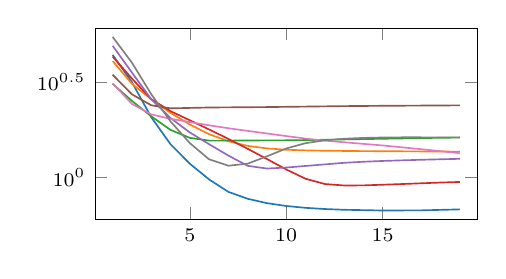
\begin{tikzpicture}

\definecolor{crimson2143940}{RGB}{214,39,40}
\definecolor{darkgray176}{RGB}{176,176,176}
\definecolor{darkorange25512714}{RGB}{255,127,14}
\definecolor{forestgreen4416044}{RGB}{44,160,44}
\definecolor{gray127}{RGB}{127,127,127}
\definecolor{mediumpurple148103189}{RGB}{148,103,189}
\definecolor{orchid227119194}{RGB}{227,119,194}
\definecolor{sienna1408675}{RGB}{140,86,75}
\definecolor{steelblue31119180}{RGB}{31,119,180}

\begin{axis}[compar,
	ymode=log]
\addplot [semithick, steelblue31119180]
table {%
0 0
1 4.39749574661255
2 3.16256737709045
3 2.07332468032837
4 1.49553334712982
5 1.18214440345764
6 0.977179050445557
7 0.841143608093262
8 0.773991823196411
9 0.734245896339417
10 0.709366321563721
11 0.693759083747864
12 0.683870077133179
13 0.677572250366211
15 0.671758413314819
17 0.672876119613647
19 0.68084442615509
};
\addplot [semithick, darkorange25512714]
table {%
0 0
1 4.08323669433594
2 3.10199475288391
3 2.57547664642334
4 2.18336200714111
5 1.89825642108917
6 1.68810415267944
7 1.54936516284943
8 1.46627962589264
9 1.42163968086243
10 1.39940583705902
11 1.38812398910522
12 1.381991147995
14 1.37605774402618
19 1.36743998527527
};
\addplot [semithick, forestgreen4416044]
table {%
0 0
1 3.10141396522522
2 2.52339649200439
3 2.09553599357605
4 1.77827620506287
5 1.61515009403229
6 1.56184554100037
7 1.56192827224731
8 1.56496429443359
10 1.56760478019714
12 1.57824468612671
18 1.61674666404724
19 1.62057650089264
};
\addplot [semithick, crimson2143940]
table {%
0 0
1 4.30938053131104
2 3.30405259132385
3 2.57786464691162
4 2.22967576980591
5 1.99751842021942
6 1.78705489635468
7 1.59454119205475
8 1.41537261009216
9 1.25089371204376
10 1.10245156288147
11 0.985825538635254
12 0.924786567687988
13 0.908674001693726
14 0.909671068191528
16 0.924581289291382
18 0.941459655761719
19 0.948395252227783
};
\addplot [semithick, mediumpurple148103189]
table {%
0 0
1 4.90979480743408
2 3.55392289161682
3 2.57458519935608
4 2.05263900756836
5 1.72432708740234
6 1.49601340293884
7 1.30391025543213
8 1.15194547176361
9 1.11501789093018
10 1.12844049930573
13 1.19477999210358
14 1.21023106575012
15 1.22193717956543
17 1.23954260349274
19 1.25378620624542
};
\addplot [semithick, sienna1408675]
table {%
0 0
1 3.46030783653259
2 2.7321982383728
3 2.39298224449158
4 2.30667018890381
6 2.33030772209167
9 2.34230852127075
13 2.36923551559448
15 2.37843608856201
18 2.38810658454895
19 2.39077997207642
};
\addplot [semithick, orchid227119194]
table {%
0 0
1 3.11877727508545
2 2.43209671974182
3 2.14522409439087
4 2.03151178359985
5 1.95412123203278
6 1.87923157215118
7 1.81407785415649
8 1.75724256038666
10 1.65027940273285
11 1.60149526596069
12 1.56172096729279
13 1.53105866909027
15 1.47341394424438
17 1.40825009346008
19 1.34137606620789
};
\addplot [semithick, gray127]
table {%
0 0
1 5.46573209762573
2 4.00377368927002
3 2.73754954338074
4 1.97035527229309
5 1.51595783233643
6 1.24627876281738
7 1.15324974060059
8 1.18260192871094
9 1.29196572303772
10 1.42099511623383
11 1.51432955265045
12 1.56789743900299
13 1.59766149520874
14 1.61410331726074
15 1.62235808372498
16 1.62557876110077
18 1.62518692016602
19 1.62393188476562
};
\end{axis}

\end{tikzpicture}
}
&
\multicolumn{5}{c}{% This file was created with tikzplotlib v0.10.1.
\begin{tikzpicture}

\definecolor{crimson2143940}{RGB}{214,39,40}
\definecolor{darkgray176}{RGB}{176,176,176}
\definecolor{darkorange25512714}{RGB}{255,127,14}
\definecolor{forestgreen4416044}{RGB}{44,160,44}
\definecolor{gray127}{RGB}{127,127,127}
\definecolor{mediumpurple148103189}{RGB}{148,103,189}
\definecolor{orchid227119194}{RGB}{227,119,194}
\definecolor{sienna1408675}{RGB}{140,86,75}
\definecolor{steelblue31119180}{RGB}{31,119,180}

\begin{axis}[
height=\figheight,
tick align=outside,
tick pos=left,
width=\figwidth,
x grid style={darkgray176},
xmin=-0.95, xmax=19.95,
xtick style={color=black},
y grid style={darkgray176},
ymin=7.60107898712158, ymax=25.3973379135132,
ytick style={color=black}
]
\addplot [semithick, steelblue31119180]
table {%
0 9.69999980926514
1 10.1099996566772
2 12.5699996948242
3 14.8999996185303
4 16.9099998474121
5 18.8299999237061
6 20.5599994659424
7 21.7800006866455
8 22.4799995422363
9 22.8600006103516
10 23.0499992370605
11 23.1399993896484
12 23.1800003051758
13 23.1900005340576
14 23.1700000762939
15 23.1200008392334
16 23.0599994659424
17 22.9699993133545
18 22.8600006103516
19 22.7399997711182
};
\addplot [semithick, darkorange25512714]
table {%
0 10.4099998474121
1 10.3500003814697
2 11.8900003433228
3 12.9200000762939
4 13.6400003433228
5 14.1899995803833
6 14.5699996948242
7 14.8299999237061
8 15
9 15.1099996566772
10 15.210000038147
12 15.3500003814697
13 15.4099998474121
14 15.460000038147
15 15.5
16 15.5299997329712
18 15.5699996948242
19 15.5699996948242
};
\addplot [semithick, forestgreen4416044]
table {%
0 12.6199998855591
1 12.75
2 14.210000038147
3 15.4300003051758
4 16.3099994659424
5 16.6499996185303
6 16.6499996185303
9 16.2900009155273
10 16.2099990844727
11 16.1399993896484
14 15.9899997711182
15 15.960000038147
16 15.9200000762939
18 15.8599996566772
19 15.8400001525879
};
\addplot [semithick, crimson2143940]
table {%
0 10.1700000762939
1 10.2299995422363
2 12.1400003433228
3 13.6400003433228
4 14.6099996566772
5 15.3800001144409
6 16.1299991607666
7 16.9200000762939
9 18.6000003814697
10 19.2999992370605
11 19.6800003051758
12 19.8199996948242
13 19.8299999237061
14 19.7900009155273
16 19.6900005340576
17 19.6499996185303
19 19.5900001525879
};
\addplot [semithick, mediumpurple148103189]
table {%
0 8.81999969482422
1 9.02000045776367
2 11.289999961853
3 13.1599998474121
4 14.460000038147
5 15.3500003814697
6 15.8999996185303
7 16.2299995422363
8 16.3899993896484
9 16.4099998474121
10 16.3799991607666
14 16.2999992370605
16 16.2399997711182
17 16.2000007629395
19 16.1000003814697
};
\addplot [semithick, sienna1408675]
table {%
0 12.8800001144409
1 12.3800001144409
2 13.6300001144409
3 14.1700000762939
4 14.289999961853
6 14.210000038147
7 14.1499996185303
8 14.0699996948242
9 13.9799995422363
10 13.8999996185303
11 13.8299999237061
12 13.7700004577637
14 13.6700000762939
17 13.5799999237061
18 13.5699996948242
19 13.5500001907349
};
\addplot [semithick, orchid227119194]
table {%
0 12.6999998092651
1 12.7600002288818
2 14.25
3 15.1999998092651
4 15.6599998474121
5 15.8599996566772
7 16.1399993896484
8 16.2700004577637
9 16.3799991607666
10 16.4699993133545
13 16.6499996185303
14 16.7299995422363
16 16.9099998474121
18 17.1299991607666
19 17.2600002288818
};
\addplot [semithick, gray127]
table {%
0 8.40999984741211
1 8.46000003814697
3 13.5900001525879
4 15.2600002288818
5 16.3199996948242
6 16.9200000762939
7 17.1399993896484
8 17.0799999237061
9 16.8600006103516
10 16.6200008392334
11 16.4500007629395
12 16.3400001525879
13 16.2900009155273
14 16.2700004577637
15 16.2700004577637
16 16.2800006866455
18 16.3199996948242
19 16.3299999237061
};
\addplot [semithick, gray]
table {%
-0.95 24.5884170532227
19.95 24.5884170532227
};
\end{axis}

\end{tikzpicture}
}
\end{tabular}
	\caption{PGD initialisée par backprojection --- sans passe-bas}
	\label{fig:PGDbackproj-s}
\end{figure}

\begin{figure}[H]\centering
	\begin{tabular}{c c c c c c c c c}
$(1)$  &  $(2)$  &  $(3)$  &  $(4)$  &  $(5)$  &  $(6)$  &  $(7)$  &  $(8)$

\\

\includegraphics[width=0.1\textwidth]{resultats/PGD/multitarget/backproj_1-init-pas=4.25_filtre=g-0.6}
&
\includegraphics[width=0.1\textwidth]{resultats/PGD/multitarget/backproj_2-init-pas=4.25_filtre=g-0.6}
&
\includegraphics[width=0.1\textwidth]{resultats/PGD/multitarget/backproj_3-init-pas=4.25_filtre=g-0.6}
&
\includegraphics[width=0.1\textwidth]{resultats/PGD/multitarget/backproj_4-init-pas=4.25_filtre=g-0.6}
&
\includegraphics[width=0.1\textwidth]{resultats/PGD/multitarget/backproj_5-init-pas=4.25_filtre=g-0.6}
&
\includegraphics[width=0.1\textwidth]{resultats/PGD/multitarget/backproj_6-init-pas=4.25_filtre=g-0.6}
&
\includegraphics[width=0.1\textwidth]{resultats/PGD/multitarget/backproj_7-init-pas=4.25_filtre=g-0.6}
&
\includegraphics[width=0.1\textwidth]{resultats/PGD/multitarget/backproj_8-init-pas=4.25_filtre=g-0.6}

\\

\includegraphics[width=0.1\textwidth]{resultats/PGD/multitarget/backproj_1-guess-pas=4.25_filtre=g-0.6}
&
\includegraphics[width=0.1\textwidth]{resultats/PGD/multitarget/backproj_2-guess-pas=4.25_filtre=g-0.6}
&
\includegraphics[width=0.1\textwidth]{resultats/PGD/multitarget/backproj_3-guess-pas=4.25_filtre=g-0.6}
&
\includegraphics[width=0.1\textwidth]{resultats/PGD/multitarget/backproj_4-guess-pas=4.25_filtre=g-0.6}
&
\includegraphics[width=0.1\textwidth]{resultats/PGD/multitarget/backproj_5-guess-pas=4.25_filtre=g-0.6}
&
\includegraphics[width=0.1\textwidth]{resultats/PGD/multitarget/backproj_6-guess-pas=4.25_filtre=g-0.6}
&
\includegraphics[width=0.1\textwidth]{resultats/PGD/multitarget/backproj_7-guess-pas=4.25_filtre=g-0.6}
&
\includegraphics[width=0.1\textwidth]{resultats/PGD/multitarget/backproj_8-guess-pas=4.25_filtre=g-0.6}

\\

\includegraphics[width=0.1\textwidth]{resultats/PGD/multitarget/backproj_1-target-pas=4.25_filtre=g-0.6}
&
\includegraphics[width=0.1\textwidth]{resultats/PGD/multitarget/backproj_2-target-pas=4.25_filtre=g-0.6}
&
\includegraphics[width=0.1\textwidth]{resultats/PGD/multitarget/backproj_3-target-pas=4.25_filtre=g-0.6}
&
\includegraphics[width=0.1\textwidth]{resultats/PGD/multitarget/backproj_4-target-pas=4.25_filtre=g-0.6}
&
\includegraphics[width=0.1\textwidth]{resultats/PGD/multitarget/backproj_5-target-pas=4.25_filtre=g-0.6}
&
\includegraphics[width=0.1\textwidth]{resultats/PGD/multitarget/backproj_6-target-pas=4.25_filtre=g-0.6}
&
\includegraphics[width=0.1\textwidth]{resultats/PGD/multitarget/backproj_7-target-pas=4.25_filtre=g-0.6}
&
\includegraphics[width=0.1\textwidth]{resultats/PGD/multitarget/backproj_8-target-pas=4.25_filtre=g-0.6}

\\ \\



\multicolumn{4}{c}{Loss}  &  \multicolumn{5}{c}{PSNR{\color{white}bbbb}}

\\

\multicolumn{4}{c}{% This file was created with tikzplotlib v0.10.1.
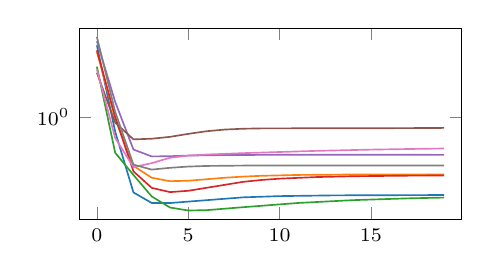
\begin{tikzpicture}

\definecolor{crimson2143940}{RGB}{214,39,40}
\definecolor{darkgray176}{RGB}{176,176,176}
\definecolor{darkorange25512714}{RGB}{255,127,14}
\definecolor{forestgreen4416044}{RGB}{44,160,44}
\definecolor{gray127}{RGB}{127,127,127}
\definecolor{mediumpurple148103189}{RGB}{148,103,189}
\definecolor{orchid227119194}{RGB}{227,119,194}
\definecolor{sienna1408675}{RGB}{140,86,75}
\definecolor{steelblue31119180}{RGB}{31,119,180}

\begin{axis}[compar,
	ymode=log]
\addplot [semithick, steelblue31119180]
table {%
0 3.70711183547974
1 0.769068241119385
2 0.254124641418457
3 0.209720253944397
4 0.209511637687683
8 0.232335805892944
10 0.237615466117859
13 0.240891814231873
19 0.242351055145264
};
\addplot [semithick, darkorange25512714]
table {%
0 3.28757643699646
1 0.976859211921692
2 0.412323236465454
3 0.332071185112
4 0.311947822570801
5 0.314504981040955
7 0.332101821899414
8 0.339040517807007
9 0.343973755836487
11 0.349475622177124
14 0.352364301681519
19 0.353339433670044
};
\addplot [semithick, forestgreen4416044]
table {%
0 2.511962890625
1 0.524079084396362
2 0.349278092384338
3 0.236259698867798
4 0.193060636520386
5 0.182855844497681
6 0.183945059776306
8 0.19417142868042
11 0.20966112613678
14 0.220738530158997
17 0.228043556213379
19 0.231406688690186
};
\addplot [semithick, crimson2143940]
table {%
0 3.3867506980896
1 1.0076789855957
2 0.373235702514648
3 0.276154518127441
4 0.255640745162964
5 0.261849880218506
8 0.308187246322632
9 0.318824410438538
10 0.32659387588501
12 0.336222290992737
14 0.341273307800293
17 0.344878911972046
19 0.346027612686157
};
\addplot [semithick, mediumpurple148103189]
table {%
0 3.99387121200562
1 1.32502341270447
2 0.555348634719849
3 0.489696025848389
4 0.491721630096436
5 0.497413158416748
7 0.502171277999878
10 0.504307508468628
16 0.504493236541748
19 0.504083871841431
};
\addplot [semithick, sienna1408675]
table {%
0 2.25173354148865
1 0.907129883766174
2 0.668294429779053
3 0.676162838935852
4 0.699749827384949
5 0.738615989685059
6 0.775098085403442
7 0.799197196960449
8 0.811239719390869
9 0.816007256507874
11 0.817354440689087
14 0.817156314849854
17 0.820295333862305
19 0.82347297668457
};
\addplot [semithick, orchid227119194]
table {%
0 2.394686460495
1 0.685625553131104
2 0.403026819229126
3 0.433403253555298
4 0.477880477905273
5 0.497187614440918
6 0.506981134414673
8 0.519890666007996
12 0.541930913925171
15 0.55438768863678
18 0.563367605209351
19 0.565675735473633
};
\addplot [semithick, gray127]
table {%
0 4.3228702545166
1 1.10458707809448
2 0.42199969291687
3 0.385361909866333
4 0.398003697395325
5 0.407153606414795
6 0.411714196205139
8 0.414519667625427
15 0.414588809013367
19 0.414569973945618
};
\end{axis}

\end{tikzpicture}
}
&
\multicolumn{5}{c}{% This file was created with tikzplotlib v0.10.1.
\begin{tikzpicture}

\definecolor{crimson2143940}{RGB}{214,39,40}
\definecolor{darkgray176}{RGB}{176,176,176}
\definecolor{darkorange25512714}{RGB}{255,127,14}
\definecolor{forestgreen4416044}{RGB}{44,160,44}
\definecolor{gray127}{RGB}{127,127,127}
\definecolor{mediumpurple148103189}{RGB}{148,103,189}
\definecolor{orchid227119194}{RGB}{227,119,194}
\definecolor{sienna1408675}{RGB}{140,86,75}
\definecolor{steelblue31119180}{RGB}{31,119,180}

\begin{axis}[
height=\figheight,
tick align=outside,
tick pos=left,
width=\figwidth,
x grid style={darkgray176},
xmin=-0.95, xmax=19.95,
xtick style={color=black},
y grid style={darkgray176},
ymin=8.07650003433228, ymax=28.3934992790222,
ytick style={color=black}
]
\addplot [semithick, steelblue31119180]
table {%
0 10.3299999237061
1 20.4699993133545
2 25.8500003814697
3 27.1800003051758
4 27.4599990844727
5 27.4699993133545
6 27.3999996185303
7 27.3199996948242
8 27.25
9 27.2000007629395
10 27.1599998474121
13 27.1000003814697
14 27.1000003814697
16 27.0799999237061
19 27.0799999237061
};
\addplot [semithick, darkorange25512714]
table {%
0 10.8999996185303
1 18.3199996948242
2 22.2999992370605
3 23.5900001525879
4 23.9500007629395
5 23.9599990844727
6 23.8700008392334
7 23.7600002288818
8 23.6700000762939
9 23.6000003814697
10 23.5499992370605
11 23.5200004577637
13 23.4799995422363
14 23.4699993133545
16 23.4699993133545
17 23.4599990844727
19 23.4599990844727
};
\addplot [semithick, forestgreen4416044]
table {%
0 13.0699996948242
1 22.0900001525879
2 24.5300006866455
3 26.0699996948242
4 26.5100002288818
5 26.4899997711182
6 26.3199996948242
7 26.1299991607666
8 25.9599990844727
9 25.8099994659424
10 25.6800003051758
11 25.5699996948242
13 25.4099998474121
14 25.3500003814697
15 25.2999992370605
16 25.2600002288818
19 25.1700000762939
};
\addplot [semithick, crimson2143940]
table {%
0 10.6300001144409
1 18.4899997711182
2 23.2099990844727
3 24.8099994659424
4 25.1499996185303
5 24.9599990844727
6 24.6200008392334
7 24.2700004577637
8 23.9799995422363
9 23.7600002288818
10 23.5900001525879
11 23.4699993133545
12 23.3700008392334
13 23.2999992370605
14 23.25
15 23.2099990844727
16 23.1800003051758
18 23.1399993896484
19 23.1299991607666
};
\addplot [semithick, mediumpurple148103189]
table {%
0 9.30000019073486
1 16.8099994659424
2 21.9799995422363
3 22.5599994659424
4 22.4099998474121
5 22.25
6 22.1499996185303
7 22.0799999237061
8 22.0300006866455
9 21.9899997711182
11 21.9500007629395
12 21.9400005340576
13 21.9400005340576
14 21.9300003051758
19 21.9300003051758
};
\addplot [semithick, sienna1408675]
table {%
0 12.6700000762939
1 17.7399997711182
2 20.1399993896484
3 19.8600006103516
4 19.3600006103516
5 18.8500003814697
6 18.4699993133545
7 18.2299995422363
8 18.1000003814697
9 18.0400009155273
10 18.0200004577637
11 18.0100002288818
13 18.0100002288818
17 17.9699993133545
19 17.9300003051758
};
\addplot [semithick, orchid227119194]
table {%
0 12.8400001525879
1 18.7999992370605
2 21.2700004577637
3 21.6599998474121
4 21.4400005340576
5 21.2000007629395
6 20.9799995422363
7 20.7700004577637
8 20.5799999237061
10 20.2600002288818
11 20.1100006103516
12 19.9699993133545
13 19.8500003814697
14 19.7399997711182
15 19.6399993896484
16 19.5499992370605
17 19.4699993133545
18 19.3999996185303
19 19.3400001525879
};
\addplot [semithick, gray127]
table {%
0 9
1 17.5100002288818
2 22.0499992370605
3 22.7600002288818
4 22.6900005340576
5 22.6000003814697
6 22.5499992370605
7 22.5200004577637
8 22.5
9 22.5
10 22.4899997711182
19 22.4899997711182
};
\addplot [semithick, gray]
table {%
-0.95 24.5884170532227
19.95 24.5884170532227
};
\end{axis}

\end{tikzpicture}
}
\end{tabular}
	\caption{PGD initialisée par backprojection --- avec passe-bas gaussien ($\sigma=0.6$)}
	\label{fig:PGDbackproj-g}
\end{figure}

\begin{figure}[H]\centering
	\begin{tabular}{c c c c c c c c c}
	$(1)$  &  $(2)$  &  $(3)$  &  $(4)$  &  $(5)$  &  $(6)$  &  $(7)$  &  $(8)$
	
	\\
	
	\includegraphics[width=0.1\textwidth]{resultats/LGD/multitarget/unif_1-init-pas=0.05_filtre=s-None}
	&
	\includegraphics[width=0.1\textwidth]{resultats/LGD/multitarget/unif_2-init-pas=0.05_filtre=s-None}
	&
	\includegraphics[width=0.1\textwidth]{resultats/LGD/multitarget/unif_3-init-pas=0.05_filtre=s-None}
	&
	\includegraphics[width=0.1\textwidth]{resultats/LGD/multitarget/unif_4-init-pas=0.05_filtre=s-None}
	&
	\includegraphics[width=0.1\textwidth]{resultats/LGD/multitarget/unif_5-init-pas=0.05_filtre=s-None}
	&
	\includegraphics[width=0.1\textwidth]{resultats/LGD/multitarget/unif_6-init-pas=0.05_filtre=s-None}
	&
	\includegraphics[width=0.1\textwidth]{resultats/LGD/multitarget/unif_7-init-pas=0.05_filtre=s-None}
	&
	\includegraphics[width=0.1\textwidth]{resultats/LGD/multitarget/unif_8-init-pas=0.05_filtre=s-None}
	
	\\
	
	\includegraphics[width=0.1\textwidth]{resultats/LGD/multitarget/unif_1-guess-pas=0.05_filtre=s-None}
	&
	\includegraphics[width=0.1\textwidth]{resultats/LGD/multitarget/unif_2-guess-pas=0.05_filtre=s-None}
	&
	\includegraphics[width=0.1\textwidth]{resultats/LGD/multitarget/unif_3-guess-pas=0.05_filtre=s-None}
	&
	\includegraphics[width=0.1\textwidth]{resultats/LGD/multitarget/unif_4-guess-pas=0.05_filtre=s-None}
	&
	\includegraphics[width=0.1\textwidth]{resultats/LGD/multitarget/unif_5-guess-pas=0.05_filtre=s-None}
	&
	\includegraphics[width=0.1\textwidth]{resultats/LGD/multitarget/unif_6-guess-pas=0.05_filtre=s-None}
	&
	\includegraphics[width=0.1\textwidth]{resultats/LGD/multitarget/unif_7-guess-pas=0.05_filtre=s-None}
	&
	\includegraphics[width=0.1\textwidth]{resultats/LGD/multitarget/unif_8-guess-pas=0.05_filtre=s-None}
	
	\\
	
	\includegraphics[width=0.1\textwidth]{resultats/LGD/multitarget/unif_1-target-pas=0.05_filtre=s-None}
	&
	\includegraphics[width=0.1\textwidth]{resultats/LGD/multitarget/unif_2-target-pas=0.05_filtre=s-None}
	&
	\includegraphics[width=0.1\textwidth]{resultats/LGD/multitarget/unif_3-target-pas=0.05_filtre=s-None}
	&
	\includegraphics[width=0.1\textwidth]{resultats/LGD/multitarget/unif_4-target-pas=0.05_filtre=s-None}
	&
	\includegraphics[width=0.1\textwidth]{resultats/LGD/multitarget/unif_5-target-pas=0.05_filtre=s-None}
	&
	\includegraphics[width=0.1\textwidth]{resultats/LGD/multitarget/unif_6-target-pas=0.05_filtre=s-None}
	&
	\includegraphics[width=0.1\textwidth]{resultats/LGD/multitarget/unif_7-target-pas=0.05_filtre=s-None}
	&
	\includegraphics[width=0.1\textwidth]{resultats/LGD/multitarget/unif_8-target-pas=0.05_filtre=s-None}
	
	\\ \\
	
	
	
	\multicolumn{4}{c}{Loss}  &  \multicolumn{5}{c}{PSNR{\color{white}bbbb}}
	
	\\
	
	\multicolumn{4}{c}{% This file was created with tikzplotlib v0.10.1.
\begin{tikzpicture}

\definecolor{crimson2143940}{RGB}{214,39,40}
\definecolor{darkgray176}{RGB}{176,176,176}
\definecolor{darkorange25512714}{RGB}{255,127,14}
\definecolor{forestgreen4416044}{RGB}{44,160,44}
\definecolor{gray127}{RGB}{127,127,127}
\definecolor{mediumpurple148103189}{RGB}{148,103,189}
\definecolor{orchid227119194}{RGB}{227,119,194}
\definecolor{sienna1408675}{RGB}{140,86,75}
\definecolor{steelblue31119180}{RGB}{31,119,180}

\begin{axis}[
height=\figheight,
tick align=outside,
tick pos=left,
width=\figwidth,
x grid style={darkgray176},
xmin=-14.95, xmax=313.95,
xtick style={color=black},
y grid style={darkgray176},
ymin=-0.182217799499631, ymax=5.67369879819453,
ytick style={color=black}
]
\addplot [semithick, steelblue31119180]
table {%
0 5.28534698486328
1 4.56153583526611
2 4.15292692184448
3 3.77370262145996
4 3.47898125648499
5 3.31976199150085
6 3.19493985176086
7 3.10722255706787
8 3.03175711631775
9 2.97216963768005
10 2.94989323616028
12 2.91763210296631
13 2.89196872711182
14 2.84459686279297
15 2.78304696083069
16 2.76125717163086
17 2.75360822677612
20 2.73654866218567
21 2.72841548919678
22 2.7157461643219
23 2.69315505027771
25 2.61465978622437
26 2.59747767448425
27 2.58550000190735
28 2.57104706764221
29 2.54467082023621
30 2.48471784591675
31 2.41675543785095
32 2.40443253517151
34 2.39707183837891
37 2.39240050315857
43 2.38842940330505
56 2.38508582115173
95 2.37702870368958
99 2.37219524383545
101 2.3663010597229
102 2.36077666282654
103 2.35122561454773
104 2.33280158042908
105 2.29480004310608
106 2.23531317710876
107 2.20305252075195
108 2.19411134719849
110 2.18735361099243
113 2.18347454071045
120 2.18023037910461
142 2.17671942710876
152 2.17329335212708
155 2.16992664337158
157 2.16440415382385
158 2.15848612785339
159 2.1463565826416
160 2.11564350128174
161 2.03211307525635
162 1.95217657089233
163 1.90615499019623
164 1.79179537296295
165 1.68968415260315
166 1.67894756793976
168 1.67080318927765
172 1.66327273845673
175 1.65709567070007
177 1.64831936359406
178 1.63878691196442
179 1.61808812618256
180 1.56098234653473
181 1.42287838459015
182 1.36243319511414
183 1.33858788013458
184 1.30298972129822
185 1.19579434394836
186 0.949332118034363
187 0.917175769805908
190 0.879632592201233
191 0.857038736343384
192 0.809222936630249
193 0.683176517486572
194 0.432179570198059
195 0.332457780838013
196 0.298513174057007
197 0.275679111480713
198 0.258496284484863
199 0.244974851608276
201 0.225065946578979
203 0.211152195930481
206 0.196685552597046
209 0.186670541763306
213 0.177221775054932
219 0.167648196220398
227 0.159289002418518
239 0.151263952255249
257 0.143872141838074
284 0.137304782867432
299 0.13481867313385
};
\addplot [semithick, darkorange25512714]
table {%
0 4.50131416320801
1 3.95711445808411
2 3.67994379997253
3 3.55212593078613
4 3.48827695846558
5 3.45385670661926
6 3.41005182266235
7 3.32293748855591
8 3.20924520492554
9 3.04128003120422
10 2.79263401031494
11 2.56510400772095
12 2.45271468162537
13 2.39788055419922
14 2.31529831886292
15 2.19441223144531
16 2.07752537727356
17 1.9688333272934
18 1.89682364463806
19 1.87376499176025
20 1.85760772228241
22 1.83091926574707
23 1.82071053981781
25 1.80813956260681
31 1.78046262264252
32 1.7734591960907
33 1.76414728164673
34 1.75061798095703
35 1.72844576835632
36 1.68554985523224
37 1.58604943752289
38 1.37616801261902
39 1.05395615100861
40 0.702062726020813
41 0.58890974521637
42 0.531301259994507
43 0.494812965393066
44 0.468652009963989
45 0.448300123214722
46 0.43159008026123
48 0.404909491539001
50 0.383750319480896
53 0.357998251914978
56 0.336583375930786
60 0.312110662460327
65 0.285808563232422
71 0.258890986442566
76 0.240169525146484
81 0.225087404251099
87 0.211062431335449
95 0.196824789047241
105 0.183586239814758
117 0.172252178192139
132 0.162585258483887
152 0.154121279716492
181 0.146317362785339
226 0.138709187507629
299 0.129801988601685
};
\addplot [semithick, forestgreen4416044]
table {%
0 4.47338724136353
1 3.9275074005127
2 3.47654843330383
3 3.1991856098175
4 3.07996201515198
5 3.00516390800476
6 2.92055535316467
8 2.69160628318787
9 2.54988622665405
10 2.38093900680542
11 2.20568799972534
12 2.0478630065918
13 1.9407764673233
14 1.87290275096893
15 1.82248294353485
16 1.76344203948975
17 1.67256844043732
18 1.53161752223969
19 1.44284379482269
20 1.41287267208099
21 1.39554369449615
22 1.38357353210449
24 1.3669685125351
27 1.34970653057098
32 1.3270138502121
36 1.31232845783234
40 1.30166745185852
45 1.29237055778503
52 1.28373658657074
62 1.27589654922485
79 1.2674309015274
102 1.25584721565247
109 1.2486720085144
113 1.24171185493469
116 1.2333402633667
118 1.22409927845001
119 1.21676564216614
120 1.20514059066772
121 1.18317639827728
122 1.13119554519653
123 1.0026034116745
124 0.902767896652222
125 0.873719453811646
126 0.860376596450806
127 0.852508783340454
129 0.843727469444275
132 0.837365388870239
137 0.832292079925537
147 0.827195405960083
164 0.818519115447998
167 0.813942193984985
169 0.807292699813843
170 0.800832509994507
171 0.788833022117615
172 0.761661767959595
173 0.679948568344116
174 0.433222532272339
175 0.356298446655273
176 0.338122129440308
177 0.331034660339355
179 0.322796583175659
182 0.316219449043274
187 0.310437917709351
196 0.305037021636963
214 0.29924201965332
255 0.291140198707581
299 0.282871007919312
};
\addplot [semithick, crimson2143940]
table {%
0 5.40752077102661
1 4.80597066879272
2 4.34973621368408
3 3.99502491950989
4 3.77043628692627
5 3.46941494941711
6 3.28981733322144
7 3.04488277435303
8 2.76343560218811
9 2.55216836929321
10 2.40857458114624
11 2.27203774452209
12 2.14232540130615
13 1.95633113384247
14 1.79061222076416
15 1.60597443580627
16 1.43814432621002
17 1.37066066265106
18 1.3303142786026
19 1.29934370517731
21 1.2424384355545
22 1.21000385284424
23 1.17056477069855
24 1.11592221260071
25 1.03759384155273
26 0.973942995071411
27 0.951019287109375
28 0.939494371414185
30 0.925424098968506
33 0.911274909973145
37 0.897227048873901
43 0.881175398826599
49 0.869409322738647
55 0.861672639846802
64 0.854896068572998
82 0.846638917922974
103 0.836658596992493
108 0.830847978591919
110 0.826242446899414
112 0.817450284957886
113 0.80912446975708
114 0.794094800949097
115 0.761519908905029
116 0.670065879821777
117 0.388494729995728
118 0.198593378067017
119 0.172587394714355
120 0.161874175071716
121 0.155910491943359
123 0.14928412437439
127 0.14246666431427
135 0.134658575057983
150 0.124749779701233
174 0.113229036331177
206 0.102245092391968
247 0.0924400091171265
299 0.0839601755142212
};
\addplot [semithick, mediumpurple148103189]
table {%
0 5.17525148391724
1 4.46839714050293
2 3.80240082740784
3 3.44209265708923
4 2.8909809589386
5 2.4438169002533
6 2.21504378318787
7 1.96019554138184
8 1.73629140853882
9 1.64245116710663
10 1.57516121864319
11 1.49089217185974
13 1.21304488182068
14 1.13481259346008
15 1.05267584323883
16 0.992837190628052
17 0.967523336410522
18 0.953469276428223
20 0.934060335159302
22 0.919294834136963
25 0.901761293411255
28 0.888113975524902
32 0.874915719032288
36 0.866126775741577
42 0.857444047927856
52 0.847656726837158
77 0.82517671585083
81 0.817153215408325
83 0.810553789138794
85 0.799945116043091
86 0.791765928268433
87 0.780100703239441
88 0.762548446655273
89 0.734684944152832
90 0.689247131347656
91 0.621073722839355
92 0.549208164215088
93 0.505539417266846
94 0.482447862625122
95 0.468284964561462
96 0.458671450614929
98 0.446300745010376
101 0.435381889343262
105 0.426153421401978
112 0.414862155914307
124 0.400126934051514
141 0.383313894271851
159 0.369489431381226
181 0.356883645057678
210 0.344543933868408
249 0.332169413566589
299 0.320428729057312
};
\addplot [semithick, sienna1408675]
table {%
0 4.75643062591553
1 4.1914005279541
2 3.47525811195374
3 2.88570737838745
4 2.61973404884338
5 2.38577365875244
6 2.16668939590454
7 1.98173344135284
8 1.83440661430359
9 1.74078953266144
10 1.68478417396545
11 1.64463210105896
12 1.6110132932663
13 1.57983684539795
14 1.55150067806244
15 1.52962636947632
16 1.51454961299896
17 1.50337076187134
19 1.48675310611725
21 1.47439277172089
24 1.45991122722626
31 1.42926943302155
33 1.41640782356262
34 1.40747559070587
35 1.39526689052582
36 1.37699663639069
37 1.34645593166351
38 1.28956162929535
39 1.18561172485352
40 1.06652176380157
41 0.997581481933594
42 0.948961496353149
43 0.906554222106934
44 0.871098518371582
45 0.844008803367615
46 0.823452830314636
47 0.806931614875793
50 0.76608669757843
52 0.737357497215271
55 0.692076802253723
56 0.68034839630127
57 0.671283006668091
59 0.658873558044434
62 0.646246910095215
70 0.615732073783875
73 0.599675416946411
75 0.584678769111633
76 0.574977517127991
77 0.563131809234619
78 0.548411846160889
79 0.529876470565796
80 0.506437420845032
81 0.477160453796387
82 0.442031145095825
84 0.364915251731873
85 0.332339882850647
86 0.30746328830719
87 0.289269089698792
88 0.275739669799805
90 0.256766676902771
92 0.243579864501953
95 0.229178786277771
99 0.215105056762695
104 0.201792478561401
111 0.187622547149658
120 0.173835873603821
133 0.158452033996582
153 0.139310598373413
172 0.124820351600647
191 0.114520788192749
216 0.10539448261261
254 0.0958684682846069
299 0.0878281593322754
};
\addplot [semithick, orchid227119194]
table {%
0 3.92581963539124
1 3.62428879737854
2 3.50237894058228
4 3.29934787750244
5 3.22077679634094
6 3.17503428459167
7 3.11121678352356
8 3.02285242080688
9 2.95440888404846
10 2.88839912414551
11 2.84978413581848
12 2.79799509048462
13 2.694087266922
14 2.62791323661804
15 2.60879683494568
16 2.59960126876831
18 2.58981251716614
21 2.58129811286926
26 2.56831240653992
28 2.55806279182434
29 2.54855990409851
30 2.53228116035461
31 2.50512218475342
32 2.47463154792786
33 2.46057319641113
34 2.45607542991638
37 2.45103740692139
44 2.44611835479736
57 2.43760013580322
60 2.43288254737854
62 2.42689085006714
63 2.42199087142944
64 2.41487622261047
67 2.38373684883118
69 2.37653660774231
71 2.36821150779724
72 2.3587474822998
73 2.33697152137756
74 2.27789807319641
75 2.19410443305969
76 2.17872285842896
78 2.16747260093689
81 2.15323996543884
82 2.1449875831604
83 2.1304075717926
84 2.09984397888184
85 2.03417944908142
86 1.9649453163147
87 1.9470202922821
88 1.94024085998535
90 1.93394339084625
94 1.92891371250153
102 1.92459678649902
117 1.92115819454193
154 1.91786587238312
215 1.9126809835434
220 1.90924370288849
223 1.90314972400665
224 1.89878904819489
225 1.89139986038208
226 1.8775829076767
227 1.84988975524902
228 1.80392038822174
229 1.77495551109314
230 1.77035427093506
233 1.76810431480408
246 1.76625168323517
296 1.76444911956787
299 1.76439142227173
};
\addplot [semithick, gray127]
table {%
0 4.62645816802979
1 3.82897400856018
2 3.08408236503601
3 2.74020624160767
4 2.57154560089111
5 2.52055215835571
6 2.43933486938477
7 2.33540630340576
8 2.26016235351562
9 2.16121315956116
10 2.12668991088867
11 2.10705399513245
12 2.08516407012939
13 2.05312442779541
14 2.00198650360107
15 1.94113075733185
16 1.90422368049622
18 1.86040651798248
19 1.828782081604
20 1.7698358297348
21 1.67915534973145
22 1.63166451454163
23 1.61739706993103
24 1.60937428474426
26 1.59932458400726
30 1.58254396915436
31 1.57559275627136
32 1.56404781341553
33 1.54018616676331
34 1.47669565677643
35 1.32811915874481
36 1.27303850650787
37 1.26257264614105
39 1.25119519233704
42 1.24236702919006
47 1.23410260677338
54 1.22252595424652
56 1.2155601978302
57 1.20972204208374
58 1.2003880739212
59 1.18358397483826
60 1.14852833747864
61 1.06632125377655
62 0.925085783004761
63 0.865402698516846
64 0.853776216506958
66 0.844574213027954
69 0.838217496871948
74 0.83280622959137
83 0.827857255935669
98 0.824196815490723
133 0.820943117141724
192 0.815026998519897
203 0.810038328170776
208 0.803974270820618
211 0.795929193496704
213 0.785049915313721
214 0.77564263343811
215 0.760635256767273
216 0.734225511550903
217 0.681595325469971
218 0.564618945121765
219 0.343624830245972
220 0.187771201133728
221 0.149633288383484
222 0.136356472969055
223 0.130478620529175
225 0.125778198242188
229 0.122974395751953
244 0.119310140609741
284 0.114052653312683
299 0.11266028881073
};
\end{axis}

\end{tikzpicture}
}
	&
	\multicolumn{5}{c}{% This file was created with tikzplotlib v0.10.1.
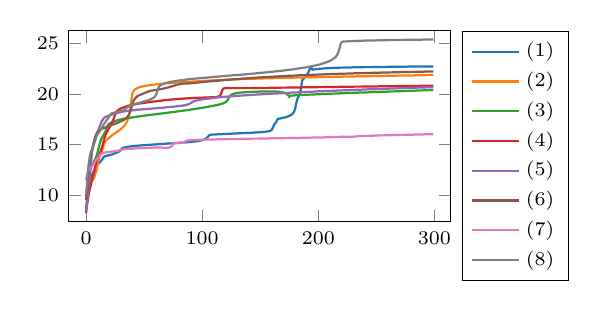
\begin{tikzpicture}

\definecolor{crimson2143940}{RGB}{214,39,40}
\definecolor{darkgray176}{RGB}{176,176,176}
\definecolor{darkorange25512714}{RGB}{255,127,14}
\definecolor{forestgreen4416044}{RGB}{44,160,44}
\definecolor{gray127}{RGB}{127,127,127}
\definecolor{mediumpurple148103189}{RGB}{148,103,189}
\definecolor{orchid227119194}{RGB}{227,119,194}
\definecolor{sienna1408675}{RGB}{140,86,75}
\definecolor{steelblue31119180}{RGB}{31,119,180}

\begin{axis}[compar, legend pos=outer north east]
\addplot [thick, steelblue31119180]
table {%
0 8.68000030517578
1 9.89999961853027
2 10.6599998474121
3 11.2799997329712
4 11.6899995803833
5 12
6 12.2600002288818
7 12.4799995422363
8 12.6899995803833
9 12.9099998474121
10 13.0600004196167
11 13.1700000762939
12 13.289999961853
13 13.4200000762939
14 13.5900001525879
15 13.7700004577637
16 13.8500003814697
17 13.8900003433228
19 13.9499998092651
20 13.9700002670288
22 14.0299997329712
23 14.0699996948242
25 14.1700000762939
26 14.210000038147
28 14.3100004196167
29 14.3800001144409
30 14.4899997711182
31 14.6400003433228
32 14.6999998092651
33 14.7299995422363
37 14.8100004196167
38 14.8199996948242
39 14.8400001525879
41 14.8599996566772
42 14.8800001144409
49 14.9499998092651
50 14.9499998092651
55 15
56 15
59 15.0299997329712
60 15.0299997329712
63 15.0600004196167
64 15.0600004196167
66 15.0799999237061
67 15.0799999237061
70 15.1099996566772
71 15.1099996566772
73 15.1300001144409
74 15.1300001144409
77 15.1599998474121
78 15.1599998474121
83 15.210000038147
84 15.210000038147
91 15.2799997329712
92 15.3000001907349
94 15.3199996948242
95 15.3400001525879
96 15.3500003814697
98 15.3900003433228
101 15.4799995422363
102 15.5299997329712
103 15.5900001525879
104 15.6700000762939
105 15.789999961853
106 15.9200000762939
107 15.9799995422363
109 16
110 16
111 16.0100002288818
112 16.0100002288818
114 16.0300006866455
115 16.0300006866455
116 16.0400009155273
117 16.0400009155273
118 16.0499992370605
119 16.0499992370605
120 16.0599994659424
121 16.0599994659424
122 16.0699996948242
123 16.0699996948242
124 16.0799999237061
125 16.0799999237061
127 16.1000003814697
128 16.1000003814697
129 16.1100006103516
130 16.1100006103516
131 16.1200008392334
132 16.1200008392334
133 16.1299991607666
134 16.1299991607666
135 16.1399993896484
136 16.1399993896484
137 16.1499996185303
138 16.1499996185303
139 16.1599998474121
140 16.1599998474121
142 16.1800003051758
143 16.1800003051758
145 16.2000007629395
146 16.2000007629395
149 16.2299995422363
150 16.2299995422363
154 16.2700004577637
155 16.2900009155273
156 16.2999992370605
157 16.3199996948242
158 16.3500003814697
159 16.3899993896484
160 16.4799995422363
161 16.7099990844727
162 17
163 17.1100006103516
164 17.2900009155273
165 17.5300006866455
166 17.5599994659424
167 17.5799999237061
168 17.6100006103516
169 17.6299991607666
170 17.6599998474121
171 17.6800003051758
172 17.7099990844727
175 17.8299999237061
176 17.8899993896484
177 17.9599990844727
178 18.0599994659424
179 18.2199993133545
180 18.5100002288818
181 19.0799999237061
182 19.5200004577637
183 19.7199993133545
184 20
185 20.4899997711182
186 21.2999992370605
187 21.4699993133545
188 21.5699996948242
189 21.6800003051758
190 21.8299999237061
191 22.0200004577637
192 22.2700004577637
193 22.5599994659424
194 22.5699996948242
195 22.3899993896484
196 22.3999996185303
197 22.4200000762939
198 22.4300003051758
199 22.4500007629395
207 22.5300006866455
208 22.5300006866455
210 22.5499992370605
211 22.5499992370605
212 22.5599994659424
213 22.5599994659424
214 22.5699996948242
215 22.5699996948242
216 22.5799999237061
218 22.5799999237061
219 22.5900001525879
221 22.5900001525879
222 22.6000003814697
225 22.6000003814697
226 22.6100006103516
229 22.6100006103516
230 22.6200008392334
233 22.6200008392334
234 22.6299991607666
239 22.6299991607666
240 22.6399993896484
245 22.6399993896484
246 22.6499996185303
251 22.6499996185303
252 22.6599998474121
259 22.6599998474121
260 22.6700000762939
267 22.6700000762939
268 22.6800003051758
276 22.6800003051758
277 22.6900005340576
286 22.6900005340576
287 22.7000007629395
297 22.7000007629395
298 22.7099990844727
299 22.7099990844727
};
\addlegendentry{\scriptsize{$(1)$}}
\addplot [thick, darkorange25512714]
table {%
0 9.68000030517578
1 10.539999961853
2 10.960000038147
3 11.1499996185303
4 11.289999961853
5 11.4099998474121
6 11.5500001907349
7 11.789999961853
8 12.1199998855591
9 12.4799995422363
11 13.6400003433228
12 14.0299997329712
13 14.25
14 14.5100002288818
15 14.9200000762939
16 15.2200002670288
17 15.3800001144409
18 15.5200004577637
19 15.6099996566772
20 15.6899995803833
21 15.7799997329712
23 15.9799995422363
25 16.1399993896484
26 16.2099990844727
29 16.4500007629395
30 16.5400009155273
31 16.6399993896484
32 16.75
33 16.8799991607666
34 17.0300006866455
35 17.2299995422363
36 17.5
37 17.9200000762939
38 18.6000003814697
39 19.4300003051758
40 20.1200008392334
41 20.3199996948242
42 20.4400005340576
43 20.5100002288818
44 20.5699996948242
45 20.6200008392334
46 20.6599998474121
48 20.7199993133545
49 20.7399997711182
50 20.7700004577637
54 20.8500003814697
55 20.8600006103516
57 20.8999996185303
59 20.9200000762939
60 20.9400005340576
63 20.9699993133545
64 20.9899997711182
73 21.0799999237061
74 21.0799999237061
79 21.1299991607666
80 21.1299991607666
83 21.1599998474121
84 21.1599998474121
87 21.1900005340576
88 21.1900005340576
90 21.2099990844727
91 21.2099990844727
93 21.2299995422363
94 21.2299995422363
96 21.25
97 21.25
99 21.2700004577637
100 21.2700004577637
102 21.2900009155273
103 21.2900009155273
105 21.3099994659424
106 21.3099994659424
107 21.3199996948242
108 21.3199996948242
110 21.3400001525879
111 21.3400001525879
112 21.3500003814697
113 21.3500003814697
115 21.3700008392334
116 21.3700008392334
117 21.3799991607666
118 21.3799991607666
119 21.3899993896484
120 21.3899993896484
121 21.3999996185303
122 21.3999996185303
123 21.4099998474121
124 21.4099998474121
125 21.4200000762939
126 21.4200000762939
127 21.4300003051758
128 21.4300003051758
129 21.4400005340576
131 21.4400005340576
132 21.4500007629395
133 21.4500007629395
134 21.4599990844727
135 21.4599990844727
136 21.4699993133545
138 21.4699993133545
139 21.4799995422363
140 21.4799995422363
141 21.4899997711182
143 21.4899997711182
144 21.5
146 21.5
147 21.5100002288818
149 21.5100002288818
150 21.5200004577637
152 21.5200004577637
153 21.5300006866455
155 21.5300006866455
156 21.5400009155273
158 21.5400009155273
159 21.5499992370605
161 21.5499992370605
162 21.5599994659424
164 21.5599994659424
165 21.5699996948242
168 21.5699996948242
169 21.5799999237061
171 21.5799999237061
172 21.5900001525879
175 21.5900001525879
176 21.6000003814697
179 21.6000003814697
180 21.6100006103516
182 21.6100006103516
183 21.6200008392334
186 21.6200008392334
187 21.6299991607666
190 21.6299991607666
191 21.6399993896484
195 21.6399993896484
196 21.6499996185303
199 21.6499996185303
200 21.6599998474121
203 21.6599998474121
204 21.6700000762939
208 21.6700000762939
209 21.6800003051758
212 21.6800003051758
213 21.6900005340576
217 21.6900005340576
218 21.7000007629395
221 21.7000007629395
222 21.7099990844727
226 21.7099990844727
227 21.7199993133545
231 21.7199993133545
232 21.7299995422363
236 21.7299995422363
237 21.7399997711182
241 21.7399997711182
242 21.75
246 21.75
247 21.7600002288818
251 21.7600002288818
252 21.7700004577637
256 21.7700004577637
257 21.7800006866455
261 21.7800006866455
262 21.7900009155273
266 21.7900009155273
267 21.7999992370605
271 21.7999992370605
272 21.8099994659424
276 21.8099994659424
277 21.8199996948242
282 21.8199996948242
283 21.8299999237061
287 21.8299999237061
288 21.8400001525879
292 21.8400001525879
293 21.8500003814697
297 21.8500003814697
298 21.8600006103516
299 21.8600006103516
};
\addlegendentry{\scriptsize{$(2)$}}
\addplot [thick, forestgreen4416044]
table {%
0 9.94999980926514
1 10.8699998855591
2 11.7399997711182
3 12.3800001144409
4 12.6800003051758
5 12.9300003051758
6 13.1499996185303
7 13.3999996185303
8 13.6099996566772
9 13.8999996185303
10 14.2799997329712
12 15.2200002670288
13 15.5500001907349
14 15.7600002288818
15 15.9399995803833
16 16.1399993896484
17 16.4099998474121
18 16.75
19 16.9899997711182
20 17.0699996948242
21 17.1399993896484
24 17.2900009155273
26 17.3700008392334
27 17.3999996185303
28 17.4400005340576
29 17.4699993133545
30 17.4899997711182
31 17.5200004577637
36 17.6200008392334
37 17.6299991607666
41 17.7099990844727
42 17.7199993133545
45 17.7800006866455
46 17.7900009155273
47 17.8099994659424
48 17.8199996948242
49 17.8400001525879
50 17.8500003814697
52 17.8899993896484
53 17.8999996185303
54 17.9200000762939
55 17.9300003051758
56 17.9500007629395
58 17.9699993133545
59 17.9899997711182
60 18
61 18.0200004577637
62 18.0300006866455
63 18.0499992370605
64 18.0599994659424
65 18.0799999237061
67 18.1000003814697
68 18.1200008392334
69 18.1299991607666
70 18.1499996185303
71 18.1599998474121
72 18.1800003051758
73 18.1900005340576
74 18.2099990844727
75 18.2199993133545
76 18.2399997711182
77 18.25
78 18.2700004577637
79 18.2800006866455
80 18.2999992370605
81 18.3099994659424
82 18.3299999237061
83 18.3400001525879
84 18.3600006103516
85 18.3700008392334
87 18.4099998474121
88 18.4200000762939
90 18.4599990844727
91 18.4699993133545
93 18.5100002288818
94 18.5200004577637
99 18.6200008392334
100 18.6299991607666
105 18.7299995422363
106 18.7600002288818
110 18.8400001525879
111 18.8700008392334
112 18.8899993896484
113 18.9200000762939
114 18.9400005340576
117 19.0300006866455
118 19.0699996948242
119 19.1200008392334
120 19.1800003051758
121 19.2700004577637
122 19.4099998474121
123 19.6299991607666
124 19.8099994659424
125 19.9099998474121
126 19.9699993133545
127 20.0100002288818
129 20.0699996948242
131 20.1100006103516
138 20.1800003051758
139 20.1800003051758
140 20.1900005340576
141 20.1900005340576
143 20.2099990844727
145 20.2099990844727
146 20.2199993133545
148 20.2199993133545
149 20.2299995422363
151 20.2299995422363
152 20.2399997711182
162 20.2399997711182
163 20.2299995422363
164 20.2299995422363
167 20.2000007629395
170 20.1399993896484
171 20.1000003814697
173 19.9799995422363
174 19.8899993896484
175 19.7199993133545
176 19.8199996948242
180 19.8600006103516
181 19.8600006103516
183 19.8799991607666
184 19.8799991607666
185 19.8899993896484
186 19.8899993896484
188 19.9099998474121
189 19.9099998474121
190 19.9200000762939
191 19.9200000762939
192 19.9300003051758
193 19.9300003051758
194 19.9400005340576
195 19.9400005340576
196 19.9500007629395
197 19.9500007629395
198 19.9599990844727
199 19.9599990844727
200 19.9699993133545
201 19.9699993133545
202 19.9799995422363
203 19.9799995422363
204 19.9899997711182
205 19.9899997711182
206 20
207 20
208 20.0100002288818
209 20.0100002288818
210 20.0200004577637
211 20.0200004577637
212 20.0300006866455
214 20.0300006866455
215 20.0400009155273
216 20.0400009155273
217 20.0499992370605
218 20.0499992370605
219 20.0599994659424
220 20.0599994659424
221 20.0699996948242
223 20.0699996948242
224 20.0799999237061
225 20.0799999237061
226 20.0900001525879
227 20.0900001525879
228 20.1000003814697
230 20.1000003814697
231 20.1100006103516
232 20.1100006103516
233 20.1200008392334
234 20.1200008392334
235 20.1299991607666
237 20.1299991607666
238 20.1399993896484
239 20.1399993896484
240 20.1499996185303
242 20.1499996185303
243 20.1599998474121
244 20.1599998474121
245 20.1700000762939
246 20.1700000762939
247 20.1800003051758
249 20.1800003051758
250 20.1900005340576
251 20.1900005340576
252 20.2000007629395
254 20.2000007629395
255 20.2099990844727
256 20.2099990844727
257 20.2199993133545
259 20.2199993133545
260 20.2299995422363
261 20.2299995422363
262 20.2399997711182
263 20.2399997711182
264 20.25
266 20.25
267 20.2600002288818
268 20.2600002288818
269 20.2700004577637
271 20.2700004577637
272 20.2800006866455
273 20.2800006866455
274 20.2900009155273
275 20.2900009155273
276 20.2999992370605
278 20.2999992370605
279 20.3099994659424
280 20.3099994659424
281 20.3199996948242
283 20.3199996948242
284 20.3299999237061
285 20.3299999237061
286 20.3400001525879
287 20.3400001525879
288 20.3500003814697
290 20.3500003814697
291 20.3600006103516
292 20.3600006103516
293 20.3700008392334
294 20.3700008392334
295 20.3799991607666
296 20.3799991607666
297 20.3899993896484
299 20.3899993896484
};
\addlegendentry{\scriptsize{$(3)$}}
\addplot [thick, crimson2143940]
table {%
0 8.27000045776367
1 9.25
3 10.5799999237061
4 11
5 11.5799999237061
6 11.9499998092651
7 12.3699998855591
8 12.9300003051758
9 13.3699998855591
10 13.6599998474121
11 13.8999996185303
12 14.1599998474121
13 14.5200004577637
14 14.8699998855591
16 15.710000038147
17 16.0300006866455
19 16.4699993133545
20 16.6700000762939
21 16.8799991607666
22 17.1000003814697
23 17.3500003814697
24 17.6299991607666
25 17.9599990844727
26 18.2299995422363
27 18.3600006103516
28 18.4400005340576
29 18.5100002288818
30 18.5699996948242
32 18.6700000762939
35 18.7900009155273
39 18.9099998474121
41 18.9500007629395
42 18.9799995422363
46 19.0599994659424
47 19.0699996948242
49 19.1100006103516
50 19.1200008392334
52 19.1599998474121
53 19.1700000762939
54 19.1900005340576
55 19.2000007629395
56 19.2199993133545
57 19.2299995422363
58 19.25
59 19.2600002288818
60 19.2800006866455
61 19.2900009155273
62 19.3099994659424
64 19.3299999237061
65 19.3500003814697
67 19.3700008392334
68 19.3899993896484
81 19.5200004577637
82 19.5200004577637
85 19.5499992370605
86 19.5499992370605
88 19.5699996948242
89 19.5699996948242
91 19.5900001525879
92 19.5900001525879
93 19.6000003814697
94 19.6000003814697
95 19.6100006103516
96 19.6100006103516
97 19.6200008392334
98 19.6200008392334
99 19.6299991607666
100 19.6299991607666
101 19.6399993896484
102 19.6399993896484
103 19.6499996185303
104 19.6499996185303
105 19.6599998474121
106 19.6599998474121
107 19.6700000762939
108 19.6700000762939
109 19.6800003051758
110 19.6800003051758
112 19.7000007629395
113 19.7199993133545
114 19.75
115 19.7999992370605
116 19.9400005340576
117 20.2800006866455
118 20.5200004577637
119 20.5499992370605
120 20.5699996948242
121 20.5699996948242
122 20.5799999237061
123 20.5799999237061
124 20.5699996948242
142 20.5699996948242
143 20.5799999237061
149 20.5799999237061
150 20.5900001525879
156 20.5900001525879
157 20.6000003814697
162 20.6000003814697
163 20.6100006103516
167 20.6100006103516
168 20.6200008392334
173 20.6200008392334
174 20.6299991607666
179 20.6299991607666
180 20.6399993896484
185 20.6399993896484
186 20.6499996185303
191 20.6499996185303
192 20.6599998474121
198 20.6599998474121
199 20.6700000762939
204 20.6700000762939
205 20.6800003051758
210 20.6800003051758
211 20.6900005340576
217 20.6900005340576
218 20.7000007629395
223 20.7000007629395
224 20.7099990844727
230 20.7099990844727
231 20.7199993133545
237 20.7199993133545
238 20.7299995422363
244 20.7299995422363
245 20.7399997711182
251 20.7399997711182
252 20.75
258 20.75
259 20.7600002288818
265 20.7600002288818
266 20.7700004577637
272 20.7700004577637
273 20.7800006866455
279 20.7800006866455
280 20.7900009155273
286 20.7900009155273
287 20.7999992370605
294 20.7999992370605
295 20.8099994659424
299 20.8099994659424
};
\addlegendentry{\scriptsize{$(4)$}}
\addplot [thick, mediumpurple148103189]
table {%
0 8.46000003814697
1 9.48999977111816
2 10.7399997711182
3 11.5
4 12.8900003433228
5 14.2299995422363
6 14.7799997329712
7 15.25
8 15.7600002288818
9 16.0599994659424
10 16.2999992370605
11 16.5499992370605
12 16.8799991607666
13 17.2000007629395
14 17.3999996185303
15 17.5699996948242
16 17.6900005340576
17 17.75
18 17.7999992370605
23 18
24 18.0300006866455
25 18.0699996948242
29 18.1900005340576
30 18.2099990844727
31 18.2399997711182
35 18.3199996948242
36 18.3299999237061
37 18.3500003814697
38 18.3600006103516
39 18.3799991607666
42 18.4099998474121
43 18.4300003051758
50 18.5
51 18.5
63 18.6200008392334
64 18.6200008392334
68 18.6599998474121
69 18.6800003051758
76 18.75
77 18.7700004577637
79 18.7900009155273
80 18.8099994659424
81 18.8199996948242
83 18.8600006103516
84 18.8700008392334
85 18.8899993896484
86 18.9200000762939
87 18.9400005340576
89 19.0200004577637
90 19.0799999237061
91 19.1599998474121
92 19.2299995422363
93 19.2900009155273
96 19.3799991607666
101 19.4799995422363
102 19.4899997711182
103 19.5100002288818
104 19.5200004577637
105 19.5400009155273
106 19.5499992370605
107 19.5699996948242
109 19.5900001525879
110 19.6100006103516
113 19.6399993896484
114 19.6599998474121
125 19.7700004577637
126 19.7700004577637
131 19.8199996948242
132 19.8199996948242
136 19.8600006103516
137 19.8600006103516
140 19.8899993896484
141 19.8899993896484
144 19.9200000762939
145 19.9200000762939
147 19.9400005340576
148 19.9400005340576
150 19.9599990844727
151 19.9599990844727
153 19.9799995422363
154 19.9799995422363
156 20
157 20
159 20.0200004577637
160 20.0200004577637
162 20.0400009155273
163 20.0400009155273
164 20.0499992370605
165 20.0499992370605
167 20.0699996948242
168 20.0699996948242
169 20.0799999237061
170 20.0799999237061
172 20.1000003814697
173 20.1000003814697
174 20.1100006103516
175 20.1100006103516
177 20.1299991607666
178 20.1299991607666
179 20.1399993896484
180 20.1399993896484
181 20.1499996185303
182 20.1499996185303
184 20.1700000762939
185 20.1700000762939
186 20.1800003051758
187 20.1800003051758
188 20.1900005340576
189 20.1900005340576
190 20.2000007629395
191 20.2000007629395
192 20.2099990844727
193 20.2099990844727
194 20.2199993133545
195 20.2199993133545
196 20.2299995422363
197 20.2299995422363
199 20.25
200 20.25
201 20.2600002288818
202 20.2600002288818
203 20.2700004577637
204 20.2700004577637
205 20.2800006866455
206 20.2800006866455
207 20.2900009155273
208 20.2900009155273
209 20.2999992370605
211 20.2999992370605
212 20.3099994659424
213 20.3099994659424
214 20.3199996948242
215 20.3199996948242
216 20.3299999237061
217 20.3299999237061
218 20.3400001525879
219 20.3400001525879
220 20.3500003814697
221 20.3500003814697
222 20.3600006103516
223 20.3600006103516
224 20.3700008392334
226 20.3700008392334
227 20.3799991607666
228 20.3799991607666
229 20.3899993896484
230 20.3899993896484
231 20.3999996185303
232 20.3999996185303
233 20.4099998474121
235 20.4099998474121
236 20.4200000762939
237 20.4200000762939
238 20.4300003051758
239 20.4300003051758
240 20.4400005340576
241 20.4400005340576
242 20.4500007629395
244 20.4500007629395
245 20.4599990844727
246 20.4599990844727
247 20.4699993133545
249 20.4699993133545
250 20.4799995422363
251 20.4799995422363
252 20.4899997711182
254 20.4899997711182
255 20.5
256 20.5
257 20.5100002288818
258 20.5100002288818
259 20.5200004577637
261 20.5200004577637
262 20.5300006866455
263 20.5300006866455
264 20.5400009155273
266 20.5400009155273
267 20.5499992370605
269 20.5499992370605
270 20.5599994659424
271 20.5599994659424
272 20.5699996948242
274 20.5699996948242
275 20.5799999237061
276 20.5799999237061
277 20.5900001525879
279 20.5900001525879
280 20.6000003814697
282 20.6000003814697
283 20.6100006103516
284 20.6100006103516
285 20.6200008392334
287 20.6200008392334
288 20.6299991607666
290 20.6299991607666
291 20.6399993896484
292 20.6399993896484
293 20.6499996185303
295 20.6499996185303
296 20.6599998474121
298 20.6599998474121
299 20.6700000762939
};
\addlegendentry{\scriptsize{$(5)$}}
\addplot [thick, sienna1408675]
table {%
0 9.52999973297119
1 10.4399995803833
2 11.7700004577637
3 13.039999961853
4 13.7799997329712
5 14.3900003433228
6 14.9399995803833
7 15.4099998474121
8 15.8000001907349
9 16.0699996948242
10 16.2600002288818
11 16.3899993896484
12 16.4899997711182
13 16.5499992370605
14 16.6000003814697
15 16.6299991607666
17 16.7099990844727
18 16.7600002288818
19 16.7999992370605
20 16.8500003814697
21 16.8899993896484
22 16.9400005340576
25 17.0599994659424
26 17.1100006103516
27 17.1499996185303
30 17.2999992370605
32 17.4200000762939
33 17.4899997711182
34 17.5699996948242
35 17.6700000762939
36 17.7999992370605
37 17.9799995422363
38 18.2299995422363
39 18.6200008392334
40 19.0699996948242
41 19.3500003814697
42 19.5300006866455
43 19.6599998474121
44 19.7600002288818
45 19.8299999237061
47 19.9300003051758
48 19.9699993133545
50 20.0699996948242
51 20.1100006103516
53 20.2099990844727
55 20.2900009155273
56 20.3199996948242
59 20.3799991607666
60 20.3899993896484
66 20.5100002288818
67 20.5400009155273
68 20.5599994659424
72 20.6800003051758
73 20.7199993133545
75 20.7800006866455
76 20.8199996948242
77 20.8500003814697
78 20.8899993896484
81 20.9799995422363
82 21
84 21.0200004577637
87 21.0200004577637
94 21.0900001525879
95 21.1100006103516
99 21.1499996185303
100 21.1700000762939
128 21.4500007629395
129 21.4500007629395
135 21.5100002288818
136 21.5100002288818
140 21.5499992370605
141 21.5499992370605
145 21.5900001525879
146 21.5900001525879
149 21.6200008392334
150 21.6200008392334
152 21.6399993896484
153 21.6399993896484
155 21.6599998474121
156 21.6599998474121
158 21.6800003051758
159 21.6800003051758
161 21.7000007629395
162 21.7000007629395
164 21.7199993133545
165 21.7199993133545
167 21.7399997711182
168 21.7399997711182
169 21.75
170 21.75
172 21.7700004577637
173 21.7700004577637
174 21.7800006866455
175 21.7800006866455
176 21.7900009155273
177 21.7900009155273
178 21.7999992370605
179 21.7999992370605
181 21.8199996948242
182 21.8199996948242
183 21.8299999237061
184 21.8299999237061
185 21.8400001525879
186 21.8400001525879
187 21.8500003814697
188 21.8500003814697
189 21.8600006103516
190 21.8600006103516
191 21.8700008392334
193 21.8700008392334
194 21.8799991607666
195 21.8799991607666
196 21.8899993896484
197 21.8899993896484
198 21.8999996185303
199 21.8999996185303
200 21.9099998474121
202 21.9099998474121
203 21.9200000762939
204 21.9200000762939
205 21.9300003051758
206 21.9300003051758
207 21.9400005340576
209 21.9400005340576
210 21.9500007629395
211 21.9500007629395
212 21.9599990844727
214 21.9599990844727
215 21.9699993133545
216 21.9699993133545
217 21.9799995422363
219 21.9799995422363
220 21.9899997711182
222 21.9899997711182
223 22
225 22
226 22.0100002288818
228 22.0100002288818
229 22.0200004577637
230 22.0200004577637
231 22.0300006866455
233 22.0300006866455
234 22.0400009155273
236 22.0400009155273
237 22.0499992370605
240 22.0499992370605
241 22.0599994659424
243 22.0599994659424
244 22.0699996948242
246 22.0699996948242
247 22.0799999237061
249 22.0799999237061
250 22.0900001525879
253 22.0900001525879
254 22.1000003814697
256 22.1000003814697
257 22.1100006103516
260 22.1100006103516
261 22.1200008392334
263 22.1200008392334
264 22.1299991607666
267 22.1299991607666
268 22.1399993896484
271 22.1399993896484
272 22.1499996185303
275 22.1499996185303
276 22.1599998474121
279 22.1599998474121
280 22.1700000762939
283 22.1700000762939
284 22.1800003051758
287 22.1800003051758
288 22.1900005340576
291 22.1900005340576
292 22.2000007629395
295 22.2000007629395
296 22.2099990844727
299 22.2099990844727
};
\addlegendentry{\scriptsize{$(6)$}}
\addplot [thick, orchid227119194]
table {%
0 11.5100002288818
1 12.1800003051758
2 12.3999996185303
3 12.5600004196167
4 12.7399997711182
5 12.8999996185303
6 13.0299997329712
7 13.1899995803833
8 13.3800001144409
9 13.539999961853
10 13.6800003051758
11 13.789999961853
12 13.9300003051758
13 14.1099996566772
14 14.1199998855591
15 14.210000038147
16 14.2200002670288
19 14.2799997329712
20 14.289999961853
21 14.3100004196167
22 14.3199996948242
23 14.3400001525879
24 14.3500003814697
29 14.4499998092651
31 14.5100002288818
32 14.5500001907349
33 14.5699996948242
35 14.5900001525879
36 14.5900001525879
38 14.6099996566772
39 14.6099996566772
40 14.6199998855591
41 14.6199998855591
43 14.6400003433228
44 14.6400003433228
45 14.6499996185303
46 14.6499996185303
47 14.6599998474121
48 14.6599998474121
49 14.6700000762939
50 14.6700000762939
51 14.6800003051758
52 14.6800003051758
53 14.6899995803833
54 14.6899995803833
56 14.710000038147
57 14.710000038147
58 14.7200002670288
59 14.7200002670288
60 14.7299995422363
64 14.7299995422363
66 14.710000038147
67 14.6899995803833
69 14.6899995803833
71 14.710000038147
72 14.7299995422363
73 14.7799997329712
74 14.8800001144409
75 15.0799999237061
76 15.1400003433228
78 15.1800003051758
83 15.2299995422363
84 15.25
85 15.3000001907349
86 15.3800001144409
87 15.4099998474121
91 15.4499998092651
92 15.4499998092651
93 15.460000038147
94 15.460000038147
95 15.4700002670288
96 15.4700002670288
97 15.4799995422363
99 15.4799995422363
100 15.4899997711182
101 15.4899997711182
102 15.5
104 15.5
105 15.5100002288818
107 15.5100002288818
108 15.5200004577637
111 15.5200004577637
112 15.5299997329712
114 15.5299997329712
115 15.539999961853
119 15.539999961853
120 15.5500001907349
123 15.5500001907349
124 15.5600004196167
127 15.5600004196167
128 15.5699996948242
132 15.5699996948242
133 15.5799999237061
137 15.5799999237061
138 15.5900001525879
142 15.5900001525879
143 15.6000003814697
148 15.6000003814697
149 15.6099996566772
153 15.6099996566772
154 15.6199998855591
158 15.6199998855591
159 15.6300001144409
164 15.6300001144409
165 15.6400003433228
169 15.6400003433228
170 15.6499996185303
174 15.6499996185303
175 15.6599998474121
179 15.6599998474121
180 15.6700000762939
184 15.6700000762939
185 15.6800003051758
188 15.6800003051758
189 15.6899995803833
193 15.6899995803833
194 15.6999998092651
197 15.6999998092651
198 15.710000038147
200 15.710000038147
201 15.7200002670288
204 15.7200002670288
205 15.7299995422363
207 15.7299995422363
208 15.7399997711182
210 15.7399997711182
211 15.75
213 15.75
214 15.7600002288818
216 15.7600002288818
217 15.7700004577637
219 15.7700004577637
220 15.7799997329712
221 15.7799997329712
222 15.789999961853
230 15.789999961853
234 15.8299999237061
235 15.8299999237061
237 15.8500003814697
238 15.8500003814697
239 15.8599996566772
240 15.8599996566772
241 15.8699998855591
243 15.8699998855591
244 15.8800001144409
245 15.8800001144409
246 15.8900003433228
248 15.8900003433228
249 15.8999996185303
250 15.8999996185303
251 15.9099998474121
253 15.9099998474121
254 15.9200000762939
256 15.9200000762939
257 15.9300003051758
260 15.9300003051758
261 15.9399995803833
263 15.9399995803833
264 15.9499998092651
266 15.9499998092651
267 15.960000038147
270 15.960000038147
271 15.9700002670288
274 15.9700002670288
275 15.9799995422363
278 15.9799995422363
279 15.9899997711182
282 15.9899997711182
283 16
286 16
287 16.0100002288818
290 16.0100002288818
291 16.0200004577637
294 16.0200004577637
295 16.0300006866455
299 16.0300006866455
};
\addlegendentry{\scriptsize{$(7)$}}
\addplot [thick, gray127]
table {%
0 10.0299997329712
1 11.4300003051758
2 12.8699998855591
3 13.7200002670288
4 14.2799997329712
5 14.5299997329712
6 14.8000001907349
7 15.1599998474121
8 15.4700002670288
9 15.8400001525879
10 16.0499992370605
12 16.3700008392334
13 16.5400009155273
14 16.7399997711182
15 16.9599990844727
16 17.1499996185303
18 17.4500007629395
19 17.6100006103516
21 17.9899997711182
22 18.0799999237061
23 18.1200008392334
26 18.2099990844727
27 18.2299995422363
28 18.2600002288818
29 18.2800006866455
32 18.3700008392334
33 18.4300003051758
34 18.5200004577637
35 18.6599998474121
36 18.7299995422363
37 18.7900009155273
38 18.8400001525879
41 18.9599990844727
42 18.9899997711182
43 19.0300006866455
46 19.1200008392334
47 19.1599998474121
49 19.2199993133545
50 19.2600002288818
51 19.2900009155273
55 19.4500007629395
56 19.5
58 19.6200008392334
59 19.7099990844727
60 19.8600006103516
61 20.1299991607666
62 20.5499992370605
63 20.7600002288818
64 20.8400001525879
65 20.9099998474121
66 20.9599990844727
69 21.0799999237061
71 21.1399993896484
72 21.1599998474121
73 21.1900005340576
79 21.3099994659424
80 21.3199996948242
81 21.3400001525879
82 21.3500003814697
83 21.3700008392334
84 21.3799991607666
85 21.3999996185303
87 21.4200000762939
88 21.4400005340576
92 21.4799995422363
93 21.5
129 21.8600006103516
130 21.8600006103516
146 22.0200004577637
147 22.0400009155273
156 22.1299991607666
157 22.1499996185303
162 22.2000007629395
163 22.2199993133545
166 22.25
167 22.2700004577637
169 22.2900009155273
170 22.3099994659424
172 22.3299999237061
173 22.3500003814697
174 22.3600006103516
175 22.3799991607666
176 22.3899993896484
177 22.4099998474121
178 22.4200000762939
179 22.4400005340576
180 22.4500007629395
182 22.4899997711182
183 22.5
187 22.5799999237061
188 22.5900001525879
191 22.6499996185303
192 22.6800003051758
195 22.7399997711182
196 22.7700004577637
197 22.7900009155273
199 22.8500003814697
200 22.8700008392334
202 22.9300003051758
203 22.9699993133545
204 23
208 23.1599998474121
210 23.2600002288818
211 23.3199996948242
213 23.4599990844727
214 23.5499992370605
215 23.6599998474121
216 23.8099994659424
217 24.0200004577637
218 24.3700008392334
219 24.8600006103516
220 25.0900001525879
221 25.1399993896484
222 25.1599998474121
223 25.1700000762939
224 25.1700000762939
226 25.1900005340576
227 25.1900005340576
228 25.2000007629395
229 25.2000007629395
230 25.2099990844727
231 25.2099990844727
232 25.2199993133545
234 25.2199993133545
235 25.2299995422363
236 25.2299995422363
237 25.2399997711182
239 25.2399997711182
240 25.25
242 25.25
243 25.2600002288818
246 25.2600002288818
247 25.2700004577637
250 25.2700004577637
251 25.2800006866455
254 25.2800006866455
255 25.2900009155273
258 25.2900009155273
259 25.2999992370605
263 25.2999992370605
264 25.3099994659424
269 25.3099994659424
270 25.3199996948242
275 25.3199996948242
276 25.3299999237061
282 25.3299999237061
283 25.3400001525879
289 25.3400001525879
290 25.3500003814697
298 25.3500003814697
299 25.3600006103516
};
\addlegendentry{\scriptsize{$(8)$}}
\end{axis}

\end{tikzpicture}
}
\end{tabular}
	\caption{PGD initialisée suivant une loi uniforme --- sans passe-bas}
	\label{fig:PGDunif-s}
\end{figure}

\begin{figure}[H]\centering
	\begin{tabular}{c c c c c c c c c}
$(1)$  &  $(2)$  &  $(3)$  &  $(4)$  &  $(5)$  &  $(6)$  &  $(7)$  &  $(8)$
	
\\

\includegraphics[width=0.1\textwidth]{resultats/PGD/multitarget/rand_unif_1-init-pas=4.25_filtre=g-0.6}
&
\includegraphics[width=0.1\textwidth]{resultats/PGD/multitarget/rand_unif_2-init-pas=4.25_filtre=g-0.6}
&
\includegraphics[width=0.1\textwidth]{resultats/PGD/multitarget/rand_unif_3-init-pas=4.25_filtre=g-0.6}
&
\includegraphics[width=0.1\textwidth]{resultats/PGD/multitarget/rand_unif_4-init-pas=4.25_filtre=g-0.6}
&
\includegraphics[width=0.1\textwidth]{resultats/PGD/multitarget/rand_unif_5-init-pas=4.25_filtre=g-0.6}
&
\includegraphics[width=0.1\textwidth]{resultats/PGD/multitarget/rand_unif_6-init-pas=4.25_filtre=g-0.6}
&
\includegraphics[width=0.1\textwidth]{resultats/PGD/multitarget/rand_unif_7-init-pas=4.25_filtre=g-0.6}
&
\includegraphics[width=0.1\textwidth]{resultats/PGD/multitarget/rand_unif_8-init-pas=4.25_filtre=g-0.6}

\\

\includegraphics[width=0.1\textwidth]{resultats/PGD/multitarget/rand_unif_1-guess-pas=4.25_filtre=g-0.6}
&
\includegraphics[width=0.1\textwidth]{resultats/PGD/multitarget/rand_unif_2-guess-pas=4.25_filtre=g-0.6}
&
\includegraphics[width=0.1\textwidth]{resultats/PGD/multitarget/rand_unif_3-guess-pas=4.25_filtre=g-0.6}
&
\includegraphics[width=0.1\textwidth]{resultats/PGD/multitarget/rand_unif_4-guess-pas=4.25_filtre=g-0.6}
&
\includegraphics[width=0.1\textwidth]{resultats/PGD/multitarget/rand_unif_5-guess-pas=4.25_filtre=g-0.6}
&
\includegraphics[width=0.1\textwidth]{resultats/PGD/multitarget/rand_unif_6-guess-pas=4.25_filtre=g-0.6}
&
\includegraphics[width=0.1\textwidth]{resultats/PGD/multitarget/rand_unif_7-guess-pas=4.25_filtre=g-0.6}
&
\includegraphics[width=0.1\textwidth]{resultats/PGD/multitarget/rand_unif_8-guess-pas=4.25_filtre=g-0.6}

\\

\includegraphics[width=0.1\textwidth]{resultats/PGD/multitarget/rand_unif_1-target-pas=4.25_filtre=g-0.6}
&
\includegraphics[width=0.1\textwidth]{resultats/PGD/multitarget/rand_unif_2-target-pas=4.25_filtre=g-0.6}
&
\includegraphics[width=0.1\textwidth]{resultats/PGD/multitarget/rand_unif_3-target-pas=4.25_filtre=g-0.6}
&
\includegraphics[width=0.1\textwidth]{resultats/PGD/multitarget/rand_unif_4-target-pas=4.25_filtre=g-0.6}
&
\includegraphics[width=0.1\textwidth]{resultats/PGD/multitarget/rand_unif_5-target-pas=4.25_filtre=g-0.6}
&
\includegraphics[width=0.1\textwidth]{resultats/PGD/multitarget/rand_unif_6-target-pas=4.25_filtre=g-0.6}
&
\includegraphics[width=0.1\textwidth]{resultats/PGD/multitarget/rand_unif_7-target-pas=4.25_filtre=g-0.6}
&
\includegraphics[width=0.1\textwidth]{resultats/PGD/multitarget/rand_unif_8-target-pas=4.25_filtre=g-0.6}

\\ \\



\multicolumn{4}{c}{Loss}  &  \multicolumn{5}{c}{PSNR{\color{white}bbbb}}

\\

\multicolumn{4}{c}{% This file was created with tikzplotlib v0.10.1.
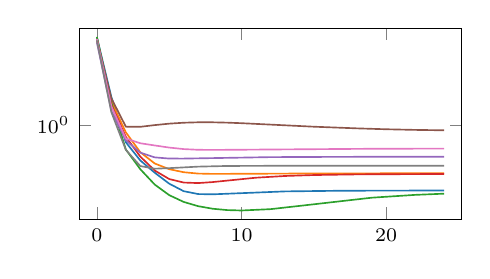
\begin{tikzpicture}

\definecolor{crimson2143940}{RGB}{214,39,40}
\definecolor{darkgray176}{RGB}{176,176,176}
\definecolor{darkorange25512714}{RGB}{255,127,14}
\definecolor{forestgreen4416044}{RGB}{44,160,44}
\definecolor{gray127}{RGB}{127,127,127}
\definecolor{mediumpurple148103189}{RGB}{148,103,189}
\definecolor{orchid227119194}{RGB}{227,119,194}
\definecolor{sienna1408675}{RGB}{140,86,75}
\definecolor{steelblue31119180}{RGB}{31,119,180}

\begin{axis}[compar,
	ymode=log]
\addplot [semithick, steelblue31119180]
table {%
0 6.6873927116394
1 1.8382842540741
2 0.689482450485229
3 0.464741587638855
4 0.356457471847534
5 0.281157732009888
6 0.238898277282715
7 0.224451065063477
8 0.223234534263611
13 0.237807869911194
17 0.24135959148407
24 0.242448091506958
};
\addplot [semithick, darkorange25512714]
table {%
0 6.45488452911377
1 1.66846358776093
2 0.854853868484497
3 0.555467844009399
4 0.435191035270691
5 0.384783029556274
6 0.360276699066162
7 0.349887132644653
8 0.34734034538269
15 0.350641131401062
24 0.352791547775269
};
\addplot [semithick, forestgreen4416044]
table {%
0 6.74908208847046
1 1.62413740158081
2 0.589171409606934
3 0.384576678276062
4 0.275595784187317
5 0.219318866729736
6 0.189371347427368
7 0.172693848609924
8 0.163402318954468
9 0.158696413040161
10 0.157270789146423
12 0.16193413734436
14 0.173686265945435
19 0.20749568939209
22 0.220578670501709
24 0.226373672485352
};
\addplot [semithick, crimson2143940]
table {%
0 6.46834373474121
1 1.53721284866333
2 0.775485038757324
3 0.505563735961914
4 0.373771667480469
5 0.310761332511902
6 0.288039445877075
7 0.284793138504028
8 0.291006684303284
11 0.319954872131348
13 0.332108616828918
15 0.338951945304871
18 0.343920707702637
24 0.346894860267639
};
\addplot [semithick, mediumpurple148103189]
table {%
0 5.98575782775879
1 1.35711002349854
2 0.718473076820374
3 0.550701856613159
4 0.496859669685364
5 0.484203457832336
6 0.483969569206238
12 0.499547839164734
17 0.50269889831543
24 0.503201842308044
};
\addplot [semithick, sienna1408675]
table {%
0 6.31420469284058
1 1.78663504123688
2 0.966158866882324
3 0.963186025619507
4 0.999682307243347
5 1.03141510486603
6 1.05243015289307
7 1.06204438209534
8 1.06177294254303
9 1.0541398525238
10 1.04162240028381
15 0.965239763259888
18 0.930991888046265
20 0.913303852081299
22 0.900914192199707
24 0.892729878425598
};
\addplot [semithick, orchid227119194]
table {%
0 6.43297863006592
1 1.49969029426575
2 0.747458696365356
3 0.67473316192627
4 0.643126964569092
5 0.61441445350647
6 0.594533920288086
7 0.585631370544434
8 0.583965182304382
19 0.598673105239868
24 0.60092830657959
};
\addplot [semithick, gray127]
table {%
0 6.25966119766235
1 1.32219290733337
2 0.585516333580017
3 0.411669135093689
4 0.388913631439209
5 0.39346170425415
7 0.406629323959351
9 0.412495374679565
13 0.414455652236938
24 0.414572954177856
};
\end{axis}

\end{tikzpicture}
}
&
\multicolumn{5}{c}{% This file was created with tikzplotlib v0.10.1.
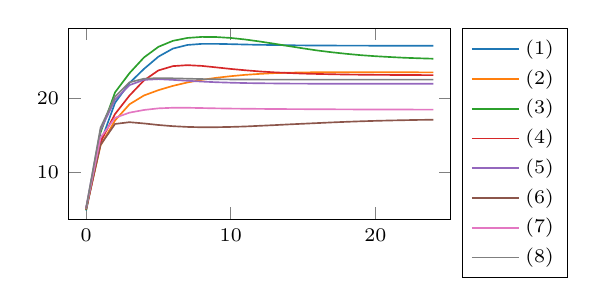
\begin{tikzpicture}

\definecolor{crimson2143940}{RGB}{214,39,40}
\definecolor{darkgray176}{RGB}{176,176,176}
\definecolor{darkorange25512714}{RGB}{255,127,14}
\definecolor{forestgreen4416044}{RGB}{44,160,44}
\definecolor{gray127}{RGB}{127,127,127}
\definecolor{mediumpurple148103189}{RGB}{148,103,189}
\definecolor{orchid227119194}{RGB}{227,119,194}
\definecolor{sienna1408675}{RGB}{140,86,75}
\definecolor{steelblue31119180}{RGB}{31,119,180}

\begin{axis}[compar, legend pos=outer north east]
\addplot [semithick, steelblue31119180]
table {%
0 4.80000019073486
1 13.9700002670288
2 19.3600006103516
3 22.0400009155273
4 23.9400005340576
5 25.6000003814697
6 26.6900005340576
7 27.1800003051758
8 27.3299999237061
9 27.3299999237061
10 27.2900009155273
11 27.2399997711182
12 27.2000007629395
14 27.1399993896484
15 27.1200008392334
18 27.0900001525879
19 27.0900001525879
20 27.0799999237061
24 27.0799999237061
 };
\addlegendentry{\scriptsize{$(1)$}}
\addplot [semithick, darkorange25512714]
table {%
0 4.94999980926514
1 13.6099996566772
2 16.9699993133545
3 19.1599998474121
4 20.3500003814697
5 21.0699996948242
6 21.6499996185303
7 22.1100006103516
8 22.4599990844727
9 22.7399997711182
10 22.9599990844727
11 23.1399993896484
12 23.2700004577637
13 23.3700008392334
14 23.4300003051758
15 23.4699993133545
16 23.4899997711182
17 23.5
20 23.5
21 23.4899997711182
22 23.4899997711182
23 23.4799995422363
24 23.4799995422363
 };
\addlegendentry{\scriptsize{$(2)$}}
\addplot [semithick, forestgreen4416044]
table {%
0 4.84000015258789
1 15.3299999237061
2 20.7700004577637
3 23.3700008392334
4 25.4899997711182
5 26.9300003051758
6 27.7399997711182
7 28.1299991607666
8 28.2700004577637
9 28.25
10 28.1299991607666
11 27.9200000762939
12 27.6499996185303
13 27.3500003814697
14 27.0300006866455
15 26.7199993133545
16 26.4300003051758
17 26.1900005340576
18 25.9799995422363
19 25.7999992370605
20 25.6599998474121
21 25.5499992370605
22 25.4500007629395
23 25.3799991607666
24 25.3199996948242
 };
\addlegendentry{\scriptsize{$(3)$}}
\addplot [semithick, crimson2143940]
table {%
0 4.94000005722046
1 14.0900001525879
2 17.8400001525879
3 20.3400001525879
4 22.3899993896484
5 23.7399997711182
6 24.3199996948242
7 24.4500007629395
8 24.3500003814697
9 24.1499996185303
10 23.9400005340576
11 23.7600002288818
12 23.6000003814697
13 23.4799995422363
14 23.3899993896484
15 23.3099994659424
16 23.2600002288818
18 23.1800003051758
20 23.1399993896484
24 23.1000003814697
 };
\addlegendentry{\scriptsize{$(4)$}}
\addplot [semithick, mediumpurple148103189]
table {%
0 5.17999982833862
1 15.6899995803833
2 19.7700004577637
3 21.75
4 22.4599990844727
5 22.5599994659424
6 22.4599990844727
7 22.3400001525879
8 22.2299995422363
9 22.1399993896484
10 22.0799999237061
11 22.0300006866455
12 22
14 21.9599990844727
16 21.9400005340576
17 21.9400005340576
18 21.9300003051758
24 21.9300003051758
 };
\addlegendentry{\scriptsize{$(5)$}}
\addplot [semithick, sienna1408675]
table {%
0 5.1100001335144
1 13.6700000762939
2 16.5
3 16.7399997711182
4 16.5699996948242
5 16.3600006103516
6 16.2000007629395
7 16.1000003814697
8 16.0499992370605
9 16.0599994659424
10 16.1000003814697
11 16.1599998474121
13 16.3400001525879
14 16.4400005340576
17 16.7099990844727
18 16.7900009155273
19 16.8600006103516
20 16.9200000762939
21 16.9699993133545
23 17.0499992370605
24 17.0699996948242
 };
\addlegendentry{\scriptsize{$(6)$}}
\addplot [semithick, orchid227119194]
table {%
0 5.05000019073486
1 14.6599998474121
2 17.3299999237061
3 18.0300006866455
4 18.3899993896484
5 18.6100006103516
6 18.6900005340576
7 18.6900005340576
9 18.6100006103516
10 18.5799999237061
13 18.5200004577637
19 18.4599990844727
20 18.4599990844727
21 18.4500007629395
22 18.4500007629395
23 18.4400005340576
24 18.4400005340576
 };
\addlegendentry{\scriptsize{$(7)$}}
\addplot [semithick, gray127]
table {%
0 5.07000017166138
1 15.9899997711182
2 20.1800003051758
3 22.1299991607666
4 22.6200008392334
5 22.7000007629395
6 22.6700000762939
8 22.5699996948242
9 22.5400009155273
10 22.5200004577637
13 22.4899997711182
24 22.4899997711182
 };
\addlegendentry{\scriptsize{$(8)$}}
\end{axis}

\end{tikzpicture}
}
\end{tabular}
	\caption{PGD initialisée suivant une loi uniforme --- avec passe-bas gaussien ($\sigma=0.6$)}
	\label{fig:PGDunif-g}
\end{figure}

\begin{figure}[H]\centering
	\begin{tabular}{c c c c c c c c c}
	$(1)$  &  $(2)$  &  $(3)$  &  $(4)$  &  $(5)$  &  $(6)$  &  $(7)$  &  $(8)$
	
	\\
	
	\includegraphics[width=0.1\textwidth]{resultats/LGD/multitarget/gauss_1-init-pas=0.05_filtre=s-None}
	&
	\includegraphics[width=0.1\textwidth]{resultats/LGD/multitarget/gauss_2-init-pas=0.05_filtre=s-None}
	&
	\includegraphics[width=0.1\textwidth]{resultats/LGD/multitarget/gauss_3-init-pas=0.05_filtre=s-None}
	&
	\includegraphics[width=0.1\textwidth]{resultats/LGD/multitarget/gauss_4-init-pas=0.05_filtre=s-None}
	&
	\includegraphics[width=0.1\textwidth]{resultats/LGD/multitarget/gauss_5-init-pas=0.05_filtre=s-None}
	&
	\includegraphics[width=0.1\textwidth]{resultats/LGD/multitarget/gauss_6-init-pas=0.05_filtre=s-None}
	&
	\includegraphics[width=0.1\textwidth]{resultats/LGD/multitarget/gauss_7-init-pas=0.05_filtre=s-None}
	&
	\includegraphics[width=0.1\textwidth]{resultats/LGD/multitarget/gauss_8-init-pas=0.05_filtre=s-None}
	
	\\
	
	\includegraphics[width=0.1\textwidth]{resultats/LGD/multitarget/gauss_1-guess-pas=0.05_filtre=s-None}
	&
	\includegraphics[width=0.1\textwidth]{resultats/LGD/multitarget/gauss_2-guess-pas=0.05_filtre=s-None}
	&
	\includegraphics[width=0.1\textwidth]{resultats/LGD/multitarget/gauss_3-guess-pas=0.05_filtre=s-None}
	&
	\includegraphics[width=0.1\textwidth]{resultats/LGD/multitarget/gauss_4-guess-pas=0.05_filtre=s-None}
	&
	\includegraphics[width=0.1\textwidth]{resultats/LGD/multitarget/gauss_5-guess-pas=0.05_filtre=s-None}
	&
	\includegraphics[width=0.1\textwidth]{resultats/LGD/multitarget/gauss_6-guess-pas=0.05_filtre=s-None}
	&
	\includegraphics[width=0.1\textwidth]{resultats/LGD/multitarget/gauss_7-guess-pas=0.05_filtre=s-None}
	&
	\includegraphics[width=0.1\textwidth]{resultats/LGD/multitarget/gauss_8-guess-pas=0.05_filtre=s-None}
	
	\\
	
	\includegraphics[width=0.1\textwidth]{resultats/LGD/multitarget/gauss_1-target-pas=0.05_filtre=s-None}
	&
	\includegraphics[width=0.1\textwidth]{resultats/LGD/multitarget/gauss_2-target-pas=0.05_filtre=s-None}
	&
	\includegraphics[width=0.1\textwidth]{resultats/LGD/multitarget/gauss_3-target-pas=0.05_filtre=s-None}
	&
	\includegraphics[width=0.1\textwidth]{resultats/LGD/multitarget/gauss_4-target-pas=0.05_filtre=s-None}
	&
	\includegraphics[width=0.1\textwidth]{resultats/LGD/multitarget/gauss_5-target-pas=0.05_filtre=s-None}
	&
	\includegraphics[width=0.1\textwidth]{resultats/LGD/multitarget/gauss_6-target-pas=0.05_filtre=s-None}
	&
	\includegraphics[width=0.1\textwidth]{resultats/LGD/multitarget/gauss_7-target-pas=0.05_filtre=s-None}
	&
	\includegraphics[width=0.1\textwidth]{resultats/LGD/multitarget/gauss_8-target-pas=0.05_filtre=s-None}
	
	\\ \\
	
	
	
	\multicolumn{4}{c}{Loss}  &  \multicolumn{5}{c}{PSNR{\color{white}bbbb}}
	
	\\
	
	\multicolumn{4}{c}{% This file was created with tikzplotlib v0.10.1.
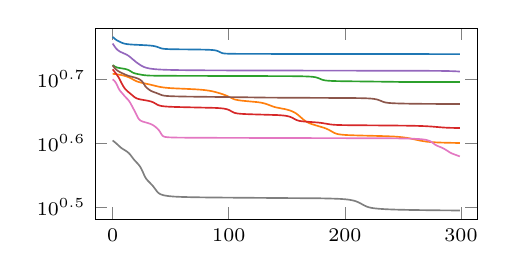
\begin{tikzpicture}

\definecolor{crimson2143940}{RGB}{214,39,40}
\definecolor{darkgray176}{RGB}{176,176,176}
\definecolor{darkorange25512714}{RGB}{255,127,14}
\definecolor{forestgreen4416044}{RGB}{44,160,44}
\definecolor{gray127}{RGB}{127,127,127}
\definecolor{mediumpurple148103189}{RGB}{148,103,189}
\definecolor{orchid227119194}{RGB}{227,119,194}
\definecolor{sienna1408675}{RGB}{140,86,75}
\definecolor{steelblue31119180}{RGB}{31,119,180}

\begin{axis}[compar,
	ymode=log]
\addplot [semithick, steelblue31119180]
table {%
0 5.83240222930908
2 5.79032802581787
3 5.7715368270874
4 5.75625896453857
5 5.74368619918823
8 5.71013402938843
9 5.70083618164062
10 5.69354677200317
11 5.6881275177002
13 5.6809983253479
15 5.67647361755371
18 5.67181062698364
25 5.66404008865356
30 5.65778398513794
33 5.65192699432373
35 5.64570951461792
36 5.64134836196899
37 5.63579702377319
38 5.62883281707764
42 5.59601020812988
43 5.59098863601685
44 5.58751821517944
46 5.58339500427246
49 5.5803656578064
54 5.57797145843506
67 5.57477807998657
78 5.5713586807251
83 5.56776475906372
86 5.56320858001709
88 5.55744743347168
89 5.55291748046875
90 5.54660320281982
91 5.53790140151978
94 5.50473403930664
95 5.49839115142822
96 5.49473667144775
98 5.49118518829346
101 5.48903131484985
107 5.48739814758301
122 5.48608160018921
167 5.48494911193848
287 5.48209428787231
299 5.48084831237793
};
\addplot [semithick, darkorange25512714]
table {%
0 5.10705995559692
3 5.0996732711792
6 5.08990049362183
8 5.08154916763306
10 5.07121419906616
12 5.05826711654663
14 5.04188919067383
16 5.02145099639893
19 4.98708391189575
20 4.97706127166748
21 4.96846437454224
22 4.96119451522827
24 4.94955158233643
27 4.93578815460205
32 4.91391515731812
36 4.89367628097534
39 4.87875080108643
41 4.87042617797852
43 4.86377954483032
46 4.85649490356445
49 4.85140752792358
54 4.84551858901978
64 4.83686351776123
71 4.82989311218262
76 4.82274198532104
79 4.81682777404785
82 4.8090500831604
85 4.79872894287109
87 4.79012155532837
89 4.78005218505859
92 4.76258087158203
95 4.74306869506836
97 4.72869920730591
99 4.71222972869873
101 4.69315147399902
103 4.67377662658691
104 4.66542816162109
105 4.65845775604248
106 4.65282726287842
108 4.64464712142944
110 4.63901901245117
113 4.63286304473877
125 4.61112260818481
127 4.60549354553223
129 4.59824228286743
131 4.58867073059082
133 4.57621002197266
139 4.5336651802063
141 4.52406215667725
144 4.51286888122559
148 4.4985523223877
150 4.48997974395752
152 4.47952175140381
154 4.46633243560791
155 4.45839977264404
156 4.44938373565674
157 4.43912982940674
158 4.42749357223511
159 4.41437768936157
160 4.39981079101562
162 4.36760425567627
164 4.33559656143188
165 4.3212194442749
166 4.30831718444824
167 4.29693078994751
168 4.28698539733887
169 4.27832889556885
171 4.26409006118774
173 4.25258636474609
182 4.20540857315063
184 4.19194412231445
186 4.17585182189941
188 4.15669393539429
190 4.13659811019897
191 4.12777137756348
192 4.1204628944397
193 4.11474704742432
194 4.11040210723877
196 4.10455369949341
199 4.09950685501099
203 4.09554719924927
210 4.0912504196167
225 4.08498525619507
236 4.07963180541992
242 4.0749683380127
246 4.07028818130493
250 4.06347894668579
253 4.05642890930176
256 4.04745721817017
260 4.03306150436401
265 4.0149712562561
268 4.00632429122925
271 3.99983978271484
275 3.99392008781433
280 3.98929643630981
287 3.9854257106781
298 3.9818172454834
299 3.98156094551086
};
\addplot [semithick, forestgreen4416044]
table {%
0 5.26967716217041
2 5.24177837371826
3 5.23101711273193
4 5.22334718704224
5 5.21792459487915
7 5.21029567718506
10 5.19987630844116
11 5.19540929794312
12 5.18981218338013
13 5.18252277374268
14 5.17289257049561
15 5.16055965423584
17 5.13293266296387
18 5.12253189086914
19 5.11513614654541
21 5.10483121871948
25 5.08837699890137
27 5.08202981948853
29 5.07777643203735
32 5.07429504394531
36 5.07217025756836
44 5.07047510147095
64 5.06902647018433
153 5.06404161453247
163 5.06113481521606
168 5.05780506134033
171 5.05394649505615
173 5.04956722259521
175 5.04227876663208
176 5.03686332702637
177 5.02987718582153
179 5.01190853118896
180 5.00302505493164
181 4.99589347839355
182 4.99071216583252
184 4.98426008224487
186 4.98045873641968
189 4.97696352005005
194 4.97377252578735
202 4.97125959396362
239 4.96241092681885
248 4.95924234390259
259 4.95839023590088
299 4.95778369903564
};
\addplot [semithick, crimson2143940]
table {%
0 5.18927192687988
2 5.13513326644897
3 5.10802888870239
4 5.07892799377441
5 5.04636383056641
6 5.00931978225708
8 4.9261417388916
9 4.88794851303101
10 4.85645389556885
11 4.83117055892944
12 4.81033802032471
13 4.79229068756104
19 4.69333171844482
20 4.68117141723633
21 4.67223310470581
22 4.66563892364502
24 4.65633773803711
27 4.64617967605591
30 4.63621664047241
32 4.62773942947388
33 4.62230539321899
34 4.61564970016479
35 4.60742521286011
36 4.59746932983398
38 4.57484483718872
39 4.56503582000732
40 4.55756521224976
41 4.55219173431396
43 4.54536819458008
45 4.54120540618896
48 4.53716039657593
53 4.53299856185913
61 4.5289363861084
88 4.51728439331055
92 4.5130934715271
95 4.50762987136841
97 4.50156545639038
98 4.49724769592285
99 4.49167251586914
100 4.48449325561523
101 4.47550296783447
104 4.44466543197632
105 4.43746042251587
106 4.43240308761597
108 4.42626428604126
111 4.42129325866699
115 4.4173002243042
122 4.41284942626953
142 4.40199899673462
146 4.39708614349365
148 4.39321231842041
150 4.38754653930664
152 4.37885332107544
153 4.3728175163269
154 4.36536741256714
155 4.35648059844971
158 4.32736492156982
159 4.31999683380127
160 4.31443071365356
161 4.31032276153564
163 4.30488920211792
166 4.3000168800354
177 4.28543663024902
180 4.2787070274353
183 4.2699236869812
187 4.25789499282837
189 4.25351810455322
192 4.24940919876099
196 4.24669647216797
203 4.24464511871338
221 4.24224519729614
251 4.23798322677612
262 4.23441553115845
269 4.23006629943848
274 4.22495651245117
279 4.21775484085083
285 4.20891857147217
289 4.20523881912231
294 4.20304584503174
299 4.20216655731201
};
\addplot [semithick, mediumpurple148103189]
table {%
0 5.69481325149536
2 5.62417125701904
3 5.59365653991699
4 5.56946468353271
5 5.55086994171143
6 5.53610944747925
7 5.52376651763916
9 5.502769947052
11 5.48242950439453
12 5.47098779678345
13 5.4578537940979
14 5.44254159927368
15 5.42506742477417
20 5.33050870895386
22 5.29755926132202
24 5.26820707321167
25 5.25528621673584
26 5.24388742446899
27 5.23411893844604
28 5.22590827941895
29 5.21906757354736
31 5.20859336853027
33 5.2011194229126
35 5.19559955596924
38 5.18967247009277
42 5.18443632125854
47 5.180251121521
54 5.17662286758423
65 5.17333841323853
82 5.17063331604004
111 5.16835117340088
169 5.16622352600098
267 5.16257762908936
283 5.16004800796509
291 5.15685176849365
295 5.15366458892822
298 5.14958047866821
299 5.14765357971191
};
\addplot [semithick, sienna1408675]
table {%
0 5.26216268539429
1 5.23293161392212
2 5.2069239616394
3 5.18563890457153
4 5.16856050491333
5 5.15438508987427
6 5.14201498031616
8 5.12022066116333
10 5.10044860839844
12 5.08227252960205
14 5.06721687316895
16 5.05559587478638
19 5.03938436508179
21 5.02572917938232
22 5.01708602905273
23 5.00663137435913
24 4.99360275268555
25 4.97656631469727
26 4.95288181304932
28 4.88731336593628
29 4.86366605758667
30 4.84542989730835
31 4.82921552658081
32 4.81494998931885
33 4.8031063079834
34 4.79350185394287
36 4.77818012237549
38 4.76373100280762
42 4.7317099571228
43 4.72591924667358
44 4.72169494628906
46 4.71645975112915
49 4.71234703063965
54 4.70870590209961
62 4.70541715621948
77 4.70175647735596
108 4.69455575942993
134 4.68720674514771
155 4.68515348434448
208 4.68019723892212
216 4.67728614807129
220 4.67426252365112
223 4.67020463943481
225 4.66576051712036
227 4.65877485275269
228 4.65386486053467
229 4.64777803421021
231 4.63240718841553
233 4.6168098449707
234 4.61078262329102
235 4.60618114471436
237 4.60013866424561
239 4.59649801254272
242 4.59305238723755
247 4.58955574035645
255 4.58629655838013
268 4.58342361450195
290 4.5810112953186
299 4.58038902282715
};
\addplot [semithick, orchid227119194]
table {%
0 5.00570917129517
1 4.98847007751465
2 4.96598672866821
3 4.93511581420898
4 4.89422702789307
5 4.84955978393555
6 4.8142352104187
7 4.78925848007202
9 4.74368858337402
10 4.72017860412598
11 4.69824695587158
13 4.65746450424194
14 4.63383388519287
15 4.60497903823853
16 4.57074451446533
18 4.49874830245972
19 4.46394348144531
20 4.4277720451355
21 4.38974952697754
22 4.35476636886597
23 4.33036804199219
24 4.3159327507019
25 4.30672836303711
26 4.29997873306274
28 4.2894115447998
31 4.27414798736572
33 4.26089191436768
34 4.2523980140686
35 4.24224185943604
36 4.23025274276733
37 4.21650552749634
38 4.20121908187866
39 4.18418598175049
40 4.16393327713013
41 4.138023853302
42 4.10835981369019
43 4.08626461029053
44 4.0754542350769
45 4.07016611099243
46 4.06712961196899
48 4.06375408172607
51 4.06121826171875
57 4.05889081954956
69 4.0570273399353
96 4.05546379089355
236 4.04934167861938
251 4.04615497589111
259 4.04250574111938
264 4.03811883926392
267 4.03355026245117
269 4.0288233757019
271 4.02158737182617
272 4.01645612716675
273 4.0098671913147
274 4.00144863128662
275 3.99101042747498
278 3.95521116256714
279 3.945955991745
281 3.93178963661194
283 3.91890001296997
285 3.90366554260254
287 3.88447785377502
290 3.85268378257751
291 3.84353089332581
292 3.83558702468872
294 3.82259774208069
299 3.79391956329346
};
\addplot [semithick, gray127]
table {%
0 4.01713132858276
2 3.99099349975586
3 3.97678804397583
7 3.91678977012634
8 3.90489077568054
10 3.88465023040771
12 3.86421728134155
13 3.85204315185547
14 3.8375461101532
15 3.82016396522522
16 3.80004405975342
18 3.75798535346985
19 3.7395236492157
22 3.68962121009827
23 3.67035341262817
24 3.64743638038635
25 3.61962389945984
26 3.58687520027161
27 3.55227041244507
28 3.52170443534851
29 3.49837756156921
30 3.48049426078796
32 3.45094561576843
34 3.42131662368774
35 3.40462374687195
36 3.38608598709106
38 3.34748673439026
39 3.33204221725464
40 3.32067012786865
41 3.31250381469727
42 3.30648565292358
44 3.29824638366699
46 3.29286003112793
49 3.28754544258118
53 3.28310084342957
59 3.2790641784668
68 3.27557039260864
82 3.27256488800049
106 3.26979780197144
179 3.26251602172852
190 3.25905561447144
196 3.25552034378052
200 3.25165796279907
203 3.24725365638733
206 3.24057698249817
208 3.23412322998047
210 3.22535848617554
212 3.21376872062683
214 3.19959783554077
217 3.17766237258911
219 3.16610598564148
221 3.1578414440155
223 3.15208148956299
226 3.14626622200012
230 3.14125466346741
236 3.13646650314331
244 3.13245320320129
256 3.12874865531921
275 3.12529683113098
299 3.12263607978821
};
\end{axis}

\end{tikzpicture}
}
	&
	\multicolumn{5}{c}{% This file was created with tikzplotlib v0.10.1.
\begin{tikzpicture}

\definecolor{crimson2143940}{RGB}{214,39,40}
\definecolor{darkgray176}{RGB}{176,176,176}
\definecolor{darkorange25512714}{RGB}{255,127,14}
\definecolor{forestgreen4416044}{RGB}{44,160,44}
\definecolor{gray127}{RGB}{127,127,127}
\definecolor{mediumpurple148103189}{RGB}{148,103,189}
\definecolor{orchid227119194}{RGB}{227,119,194}
\definecolor{sienna1408675}{RGB}{140,86,75}
\definecolor{steelblue31119180}{RGB}{31,119,180}

\begin{axis}[
height=\figheight,
tick align=outside,
tick pos=left,
width=\figwidth,
x grid style={darkgray176},
xmin=-14.95, xmax=313.95,
xtick style={color=black},
y grid style={darkgray176},
ymin=6.48264079093933, ymax=33.2645391941071,
ytick style={color=black}
]
\addplot [semithick, steelblue31119180]
table {%
0 7.69999980926514
3 7.73000001907349
4 7.73000001907349
5 7.73999977111816
6 7.73999977111816
8 7.76000022888184
9 7.76000022888184
10 7.76999998092651
11 7.76999998092651
12 7.78000020980835
15 7.78000020980835
16 7.78999996185303
19 7.78999996185303
20 7.80000019073486
24 7.80000019073486
25 7.80999994277954
29 7.80999994277954
30 7.82000017166138
33 7.82000017166138
34 7.82999992370605
36 7.82999992370605
37 7.84000015258789
39 7.84000015258789
40 7.84999990463257
42 7.84999990463257
43 7.8600001335144
54 7.8600001335144
55 7.86999988555908
71 7.86999988555908
72 7.88000011444092
80 7.88000011444092
81 7.8899998664856
85 7.8899998664856
86 7.90000009536743
87 7.90000009536743
88 7.90999984741211
89 7.90999984741211
90 7.92000007629395
91 7.92000007629395
95 7.96000003814697
97 7.96000003814697
98 7.96999979019165
105 7.96999979019165
106 7.98000001907349
125 7.98000001907349
126 7.98999977111816
172 7.98999977111816
173 8
299 8
};
\addplot [semithick, darkorange25512714]
table {%
0 9.13000011444092
4 9.13000011444092
5 9.14000034332275
8 9.14000034332275
9 9.14999961853027
11 9.14999961853027
12 9.15999984741211
13 9.15999984741211
14 9.17000007629395
15 9.17000007629395
16 9.18000030517578
17 9.18000030517578
19 9.19999980926514
20 9.19999980926514
21 9.21000003814697
22 9.21000003814697
23 9.22000026702881
24 9.22000026702881
25 9.22999954223633
27 9.22999954223633
28 9.23999977111816
29 9.23999977111816
30 9.25
31 9.25
32 9.26000022888184
33 9.26000022888184
35 9.27999973297119
36 9.27999973297119
37 9.28999996185303
38 9.28999996185303
40 9.3100004196167
41 9.3100004196167
42 9.31999969482422
43 9.31999969482422
44 9.32999992370605
46 9.32999992370605
47 9.34000015258789
49 9.34000015258789
50 9.35000038146973
52 9.35000038146973
53 9.35999965667725
55 9.35999965667725
56 9.36999988555908
59 9.36999988555908
60 9.38000011444092
62 9.38000011444092
63 9.39000034332275
65 9.39000034332275
66 9.39999961853027
68 9.39999961853027
69 9.40999984741211
71 9.40999984741211
72 9.42000007629395
73 9.42000007629395
74 9.43000030517578
76 9.43000030517578
78 9.44999980926514
79 9.44999980926514
80 9.46000003814697
81 9.46000003814697
83 9.47999954223633
84 9.47999954223633
88 9.52000045776367
89 9.52000045776367
93 9.5600004196167
94 9.5600004196167
97 9.59000015258789
98 9.59000015258789
100 9.60999965667725
101 9.60999965667725
103 9.63000011444092
104 9.63000011444092
105 9.64000034332275
106 9.64000034332275
107 9.64999961853027
109 9.64999961853027
110 9.65999984741211
112 9.65999984741211
113 9.67000007629395
115 9.67000007629395
116 9.68000030517578
118 9.68000030517578
119 9.6899995803833
121 9.6899995803833
122 9.69999980926514
123 9.69999980926514
124 9.71000003814697
125 9.71000003814697
126 9.72000026702881
127 9.72000026702881
134 9.78999996185303
135 9.8100004196167
137 9.82999992370605
138 9.85000038146973
141 9.88000011444092
142 9.88000011444092
145 9.90999984741211
146 9.90999984741211
149 9.9399995803833
150 9.9399995803833
158 10.0200004577637
159 10.039999961853
160 10.0500001907349
161 10.0699996948242
162 10.0799999237061
164 10.1199998855591
166 10.1400003433228
167 10.1599998474121
173 10.2200002670288
174 10.2200002670288
184 10.3199996948242
185 10.3400001525879
186 10.3500003814697
187 10.3699998855591
188 10.3800001144409
190 10.4200000762939
191 10.4300003051758
192 10.4499998092651
197 10.5
198 10.5
200 10.5200004577637
201 10.5200004577637
202 10.5299997329712
204 10.5299997329712
205 10.539999961853
206 10.539999961853
207 10.5500001907349
209 10.5500001907349
210 10.5600004196167
213 10.5600004196167
214 10.5699996948242
216 10.5699996948242
217 10.5799999237061
220 10.5799999237061
221 10.5900001525879
224 10.5900001525879
225 10.6000003814697
228 10.6000003814697
229 10.6099996566772
232 10.6099996566772
233 10.6199998855591
236 10.6199998855591
237 10.6300001144409
240 10.6300001144409
241 10.6400003433228
243 10.6400003433228
244 10.6499996185303
247 10.6499996185303
248 10.6599998474121
251 10.6599998474121
252 10.6700000762939
254 10.6700000762939
255 10.6800003051758
257 10.6800003051758
258 10.6899995803833
260 10.6899995803833
261 10.6999998092651
262 10.6999998092651
263 10.710000038147
265 10.710000038147
266 10.7200002670288
268 10.7200002670288
269 10.7299995422363
272 10.7299995422363
273 10.7399997711182
278 10.7399997711182
279 10.75
287 10.75
288 10.7600002288818
299 10.7600002288818
};
\addplot [semithick, forestgreen4416044]
table {%
0 8.25
5 8.30000019073486
6 8.30000019073486
8 8.31999969482422
9 8.31999969482422
10 8.32999992370605
11 8.32999992370605
18 8.39999961853027
19 8.39999961853027
20 8.40999984741211
21 8.40999984741211
22 8.42000007629395
27 8.42000007629395
28 8.43000030517578
51 8.43000030517578
52 8.4399995803833
75 8.4399995803833
76 8.44999980926514
112 8.44999980926514
113 8.46000003814697
163 8.46000003814697
164 8.47000026702881
176 8.47000026702881
177 8.47999954223633
179 8.47999954223633
180 8.48999977111816
183 8.48999977111816
184 8.5
195 8.5
196 8.51000022888184
268 8.51000022888184
269 8.52000045776367
299 8.52000045776367
};
\addplot [semithick, crimson2143940]
table {%
0 8.8100004196167
1 8.84000015258789
2 8.85999965667725
5 8.94999980926514
9 9.10999965667725
12 9.19999980926514
14 9.23999977111816
15 9.27000045776367
21 9.39000034332275
27 9.44999980926514
28 9.44999980926514
41 9.57999992370605
42 9.57999992370605
43 9.59000015258789
44 9.59000015258789
45 9.60000038146973
46 9.60000038146973
47 9.60999965667725
49 9.60999965667725
50 9.61999988555908
52 9.61999988555908
53 9.63000011444092
56 9.63000011444092
57 9.64000034332275
60 9.64000034332275
61 9.64999961853027
65 9.64999961853027
66 9.65999984741211
69 9.65999984741211
70 9.67000007629395
74 9.67000007629395
75 9.68000030517578
78 9.68000030517578
79 9.6899995803833
82 9.6899995803833
83 9.69999980926514
86 9.69999980926514
87 9.71000003814697
89 9.71000003814697
90 9.72000026702881
92 9.72000026702881
93 9.72999954223633
94 9.72999954223633
95 9.73999977111816
96 9.73999977111816
97 9.75
98 9.75
106 9.82999992370605
107 9.82999992370605
108 9.84000015258789
109 9.84000015258789
110 9.85000038146973
113 9.85000038146973
114 9.85999965667725
118 9.85999965667725
119 9.86999988555908
124 9.86999988555908
125 9.88000011444092
130 9.88000011444092
131 9.89000034332275
135 9.89000034332275
136 9.89999961853027
140 9.89999961853027
141 9.90999984741211
143 9.90999984741211
144 9.92000007629395
146 9.92000007629395
147 9.93000030517578
149 9.93000030517578
151 9.94999980926514
152 9.94999980926514
155 9.97999954223633
156 10
159 10.0299997329712
160 10.0299997329712
161 10.039999961853
165 10.039999961853
166 10.0500001907349
175 10.0500001907349
176 10.0600004196167
181 10.0600004196167
182 10.0699996948242
189 10.0699996948242
190 10.0799999237061
216 10.0799999237061
217 10.0900001525879
249 10.0900001525879
250 10.1000003814697
275 10.1000003814697
276 10.1099996566772
291 10.1099996566772
292 10.1199998855591
299 10.1199998855591
};
\addplot [semithick, mediumpurple148103189]
table {%
0 7.80999994277954
1 7.84000015258789
2 7.8600001335144
3 7.8899998664856
4 7.90000009536743
5 7.92000007629395
6 7.92999982833862
7 7.92999982833862
9 7.94999980926514
10 7.94999980926514
12 7.96999979019165
13 7.96999979019165
17 8.01000022888184
18 8.01000022888184
24 8.06999969482422
25 8.06999969482422
28 8.10000038146973
29 8.10000038146973
31 8.11999988555908
33 8.11999988555908
34 8.13000011444092
37 8.13000011444092
38 8.14000034332275
41 8.14000034332275
42 8.14999961853027
48 8.14999961853027
49 8.15999984741211
57 8.15999984741211
58 8.17000007629395
67 8.17000007629395
68 8.18000030517578
81 8.18000030517578
82 8.1899995803833
98 8.1899995803833
99 8.19999980926514
120 8.19999980926514
121 8.21000003814697
145 8.21000003814697
146 8.22000026702881
175 8.22000026702881
176 8.22999954223633
207 8.22999954223633
208 8.23999977111816
240 8.23999977111816
241 8.25
266 8.25
267 8.26000022888184
283 8.26000022888184
284 8.27000045776367
292 8.27000045776367
293 8.27999973297119
297 8.27999973297119
298 8.28999996185303
299 8.28999996185303
};
\addplot [semithick, sienna1408675]
table {%
0 8.60999965667725
3 8.72999954223633
4 8.75
5 8.77999973297119
7 8.81999969482422
8 8.82999992370605
9 8.85000038146973
11 8.86999988555908
12 8.86999988555908
13 8.88000011444092
14 8.88000011444092
15 8.89000034332275
16 8.89000034332275
18 8.90999984741211
19 8.90999984741211
23 8.94999980926514
25 8.98999977111816
27 9.05000019073486
28 9.09000015258789
29 9.11999988555908
31 9.15999984741211
35 9.19999980926514
36 9.19999980926514
37 9.21000003814697
38 9.21000003814697
39 9.22000026702881
40 9.22000026702881
41 9.22999954223633
43 9.22999954223633
44 9.23999977111816
47 9.23999977111816
48 9.25
55 9.25
56 9.26000022888184
72 9.26000022888184
73 9.27000045776367
157 9.27000045776367
158 9.27999973297119
190 9.27999973297119
191 9.27000045776367
214 9.27000045776367
215 9.26000022888184
223 9.26000022888184
224 9.25
235 9.25
236 9.26000022888184
242 9.26000022888184
243 9.27000045776367
251 9.27000045776367
252 9.27999973297119
262 9.27999973297119
263 9.28999996185303
277 9.28999996185303
278 9.30000019073486
295 9.30000019073486
296 9.3100004196167
299 9.3100004196167
};
\addplot [semithick, orchid227119194]
table {%
0 9.22000026702881
2 9.27999973297119
3 9.31999969482422
6 9.47000026702881
8 9.52999973297119
9 9.55000019073486
13 9.67000007629395
15 9.75
22 10.1000003814697
24 10.1599998474121
27 10.2200002670288
28 10.2299995422363
29 10.25
30 10.2600002288818
35 10.3599996566772
37 10.4200000762939
38 10.460000038147
39 10.4899997711182
40 10.539999961853
41 10.5799999237061
42 10.6400003433228
43 10.6800003051758
44 10.710000038147
48 10.75
49 10.75
50 10.7600002288818
51 10.7600002288818
52 10.7700004577637
54 10.7700004577637
55 10.7799997329712
58 10.7799997329712
59 10.789999961853
65 10.789999961853
66 10.8000001907349
74 10.8000001907349
75 10.8100004196167
88 10.8100004196167
89 10.8199996948242
110 10.8199996948242
111 10.8299999237061
147 10.8299999237061
148 10.8400001525879
215 10.8400001525879
216 10.8500003814697
266 10.8500003814697
267 10.8599996566772
272 10.8599996566772
273 10.8699998855591
274 10.8699998855591
276 10.8900003433228
277 10.8900003433228
279 10.9099998474121
280 10.9099998474121
281 10.9200000762939
282 10.9200000762939
283 10.9300003051758
284 10.9300003051758
297 11.0600004196167
298 11.0600004196167
299 11.0699996948242
};
\addplot [semithick, gray127]
table {%
0 11.3400001525879
1 11.3599996566772
3 11.3800001144409
4 11.3999996185303
6 11.4200000762939
7 11.4399995803833
8 11.4499998092651
9 11.4700002670288
11 11.4899997711182
15 11.5699996948242
18 11.6599998474121
19 11.6800003051758
20 11.710000038147
23 11.7700004577637
26 11.8599996566772
28 11.9399995803833
29 11.9700002670288
34 12.0699996948242
35 12.0799999237061
39 12.1599998474121
42 12.1899995803833
43 12.1899995803833
44 12.1999998092651
46 12.1999998092651
47 12.210000038147
51 12.210000038147
52 12.2200002670288
57 12.2200002670288
58 12.2299995422363
65 12.2299995422363
66 12.2399997711182
74 12.2399997711182
75 12.25
84 12.25
85 12.2600002288818
94 12.2600002288818
95 12.2700004577637
104 12.2700004577637
105 12.2799997329712
114 12.2799997329712
115 12.289999961853
124 12.289999961853
125 12.3000001907349
133 12.3000001907349
134 12.3100004196167
142 12.3100004196167
143 12.3199996948242
150 12.3199996948242
151 12.3299999237061
158 12.3299999237061
159 12.3400001525879
165 12.3400001525879
166 12.3500003814697
171 12.3500003814697
172 12.3599996566772
178 12.3599996566772
179 12.3699998855591
183 12.3699998855591
184 12.3800001144409
188 12.3800001144409
189 12.3900003433228
193 12.3900003433228
194 12.3999996185303
197 12.3999996185303
198 12.4099998474121
201 12.4099998474121
202 12.4200000762939
204 12.4200000762939
205 12.4300003051758
207 12.4300003051758
208 12.4399995803833
209 12.4399995803833
210 12.4499998092651
211 12.4499998092651
212 12.460000038147
214 12.460000038147
215 12.4700002670288
216 12.4700002670288
217 12.4799995422363
220 12.4799995422363
221 12.4899997711182
225 12.4899997711182
226 12.5
231 12.5
232 12.5100002288818
237 12.5100002288818
238 12.5200004577637
245 12.5200004577637
246 12.5299997329712
253 12.5299997329712
254 12.539999961853
263 12.539999961853
264 12.5500001907349
274 12.5500001907349
275 12.5600004196167
286 12.5600004196167
287 12.5699996948242
299 12.5699996948242
};
\addplot [semithick, gray]
table {%
-14.95 32.0471801757812
313.95 32.0471801757812
};
\end{axis}

\end{tikzpicture}
}
\end{tabular}
	\caption{PGD initialisée suivant une loi normale --- sans passe-bas}
	\label{fig:PGDgauss-s}
\end{figure}

\begin{figure}[H]\centering
	\begin{tabular}{c c c c c c c c c}
	$(1)$  &  $(2)$  &  $(3)$  &  $(4)$  &  $(5)$  &  $(6)$  &  $(7)$  &  $(8)$
	
	\\
	
	\includegraphics[width=0.1\textwidth]{resultats/LGD/multitarget/gauss_1-init-pas=0.25_filtre=g-0.6}
	&
	\includegraphics[width=0.1\textwidth]{resultats/LGD/multitarget/gauss_2-init-pas=0.25_filtre=g-0.6}
	&
	\includegraphics[width=0.1\textwidth]{resultats/LGD/multitarget/gauss_3-init-pas=0.25_filtre=g-0.6}
	&
	\includegraphics[width=0.1\textwidth]{resultats/LGD/multitarget/gauss_4-init-pas=0.25_filtre=g-0.6}
	&
	\includegraphics[width=0.1\textwidth]{resultats/LGD/multitarget/gauss_5-init-pas=0.25_filtre=g-0.6}
	&
	\includegraphics[width=0.1\textwidth]{resultats/LGD/multitarget/gauss_6-init-pas=0.25_filtre=g-0.6}
	&
	\includegraphics[width=0.1\textwidth]{resultats/LGD/multitarget/gauss_7-init-pas=0.25_filtre=g-0.6}
	&
	\includegraphics[width=0.1\textwidth]{resultats/LGD/multitarget/gauss_8-init-pas=0.25_filtre=g-0.6}
	
	\\
	
	\includegraphics[width=0.1\textwidth]{resultats/LGD/multitarget/gauss_1-guess-pas=0.25_filtre=g-0.6}
	&
	\includegraphics[width=0.1\textwidth]{resultats/LGD/multitarget/gauss_2-guess-pas=0.25_filtre=g-0.6}
	&
	\includegraphics[width=0.1\textwidth]{resultats/LGD/multitarget/gauss_3-guess-pas=0.25_filtre=g-0.6}
	&
	\includegraphics[width=0.1\textwidth]{resultats/LGD/multitarget/gauss_4-guess-pas=0.25_filtre=g-0.6}
	&
	\includegraphics[width=0.1\textwidth]{resultats/LGD/multitarget/gauss_5-guess-pas=0.25_filtre=g-0.6}
	&
	\includegraphics[width=0.1\textwidth]{resultats/LGD/multitarget/gauss_6-guess-pas=0.25_filtre=g-0.6}
	&
	\includegraphics[width=0.1\textwidth]{resultats/LGD/multitarget/gauss_7-guess-pas=0.25_filtre=g-0.6}
	&
	\includegraphics[width=0.1\textwidth]{resultats/LGD/multitarget/gauss_8-guess-pas=0.25_filtre=g-0.6}
	
	\\
	
	\includegraphics[width=0.1\textwidth]{resultats/LGD/multitarget/gauss_1-target-pas=0.25_filtre=g-0.6}
	&
	\includegraphics[width=0.1\textwidth]{resultats/LGD/multitarget/gauss_2-target-pas=0.25_filtre=g-0.6}
	&
	\includegraphics[width=0.1\textwidth]{resultats/LGD/multitarget/gauss_3-target-pas=0.25_filtre=g-0.6}
	&
	\includegraphics[width=0.1\textwidth]{resultats/LGD/multitarget/gauss_4-target-pas=0.25_filtre=g-0.6}
	&
	\includegraphics[width=0.1\textwidth]{resultats/LGD/multitarget/gauss_5-target-pas=0.25_filtre=g-0.6}
	&
	\includegraphics[width=0.1\textwidth]{resultats/LGD/multitarget/gauss_6-target-pas=0.25_filtre=g-0.6}
	&
	\includegraphics[width=0.1\textwidth]{resultats/LGD/multitarget/gauss_7-target-pas=0.25_filtre=g-0.6}
	&
	\includegraphics[width=0.1\textwidth]{resultats/LGD/multitarget/gauss_8-target-pas=0.25_filtre=g-0.6}
	
	\\ \\
	
	
	
	\multicolumn{4}{c}{Loss}  &  \multicolumn{5}{c}{PSNR{\color{white}bbbb}}
	
	\\
	
	\multicolumn{4}{c}{% This file was created with tikzplotlib v0.10.1.
\begin{tikzpicture}

\definecolor{crimson2143940}{RGB}{214,39,40}
\definecolor{darkgray176}{RGB}{176,176,176}
\definecolor{darkorange25512714}{RGB}{255,127,14}
\definecolor{forestgreen4416044}{RGB}{44,160,44}
\definecolor{gray127}{RGB}{127,127,127}
\definecolor{mediumpurple148103189}{RGB}{148,103,189}
\definecolor{orchid227119194}{RGB}{227,119,194}
\definecolor{sienna1408675}{RGB}{140,86,75}
\definecolor{steelblue31119180}{RGB}{31,119,180}

\begin{axis}[
height=\figheight,
tick align=outside,
tick pos=left,
width=\figwidth,
x grid style={darkgray176},
xmin=-14.95, xmax=313.95,
xtick style={color=black},
y grid style={darkgray176},
ymin=0.534259194135666, ymax=4.62796640992165,
ytick style={color=black}
]
\addplot [semithick, steelblue31119180]
table {%
0 4.4418888092041
1 4.38524532318115
3 4.28792333602905
5 4.19112348556519
6 4.1469259262085
7 4.10930490493774
8 4.07516717910767
9 4.03655815124512
10 3.99101114273071
11 3.94876837730408
12 3.91460013389587
13 3.88679647445679
14 3.86526942253113
15 3.84975218772888
17 3.82370185852051
18 3.80900835990906
19 3.79194402694702
21 3.75340580940247
22 3.73305320739746
23 3.71095705032349
24 3.68739891052246
25 3.66602301597595
26 3.64970731735229
27 3.6372492313385
29 3.61836266517639
33 3.5849072933197
38 3.53578400611877
40 3.50999546051025
42 3.48253178596497
45 3.44473004341125
46 3.4268045425415
47 3.40181469917297
49 3.33780026435852
50 3.30481696128845
51 3.26556468009949
52 3.21628880500793
53 3.16223955154419
54 3.11594748497009
55 3.08657431602478
57 3.03514313697815
58 3.01247715950012
59 2.99257159233093
60 2.97553300857544
61 2.96086931228638
63 2.93526935577393
66 2.89987111091614
69 2.86747193336487
72 2.83942246437073
74 2.82304239273071
77 2.80187177658081
79 2.78777766227722
80 2.77961349487305
81 2.76985144615173
82 2.75759530067444
83 2.74200081825256
84 2.72270774841309
85 2.69936466217041
86 2.66991543769836
87 2.63135552406311
88 2.59024953842163
89 2.55894374847412
90 2.53488397598267
93 2.46976280212402
95 2.42086148262024
97 2.37087845802307
98 2.34841203689575
100 2.30955219268799
102 2.27068138122559
103 2.24777770042419
104 2.22078561782837
105 2.18944025039673
109 2.05516123771667
110 2.02176237106323
111 1.98605072498322
112 1.94382536411285
113 1.8906797170639
114 1.83268594741821
115 1.78378784656525
119 1.61452889442444
120 1.57854580879211
121 1.54792296886444
122 1.5221403837204
123 1.50076627731323
124 1.48313927650452
125 1.46852040290833
126 1.45622193813324
128 1.43636655807495
130 1.42020428180695
139 1.35508036613464
141 1.3432525396347
143 1.33369064331055
146 1.32243156433105
150 1.31091260910034
155 1.29963326454163
162 1.28705406188965
171 1.27387690544128
188 1.25011670589447
190 1.24540078639984
192 1.23756670951843
193 1.2306421995163
194 1.21908235549927
195 1.19935441017151
196 1.17057466506958
197 1.13960838317871
198 1.11454939842224
199 1.09860873222351
200 1.0888614654541
201 1.0821738243103
203 1.07278609275818
206 1.06269478797913
219 1.02440273761749
229 0.985999584197998
233 0.975847363471985
239 0.964239835739136
262 0.923984169960022
267 0.911289215087891
273 0.893042922019958
280 0.868923425674438
283 0.855746150016785
285 0.843543291091919
286 0.835501432418823
287 0.825612187385559
288 0.813591122627258
291 0.77116322517395
292 0.759522795677185
293 0.750239610671997
295 0.736871957778931
297 0.727524876594543
299 0.72033679485321
};
\addplot [semithick, darkorange25512714]
table {%
0 3.52794861793518
3 3.49429416656494
6 3.46427249908447
9 3.43450284004211
11 3.41129517555237
13 3.38787579536438
14 3.37831807136536
15 3.37061429023743
17 3.35945200920105
19 3.35173010826111
22 3.34335136413574
28 3.33081650733948
33 3.3192892074585
36 3.30876135826111
38 3.29896569252014
41 3.28089714050293
48 3.23478269577026
50 3.2214789390564
52 3.21155428886414
56 3.19492864608765
59 3.18516039848328
63 3.1757960319519
71 3.15817356109619
74 3.14809679985046
76 3.13865756988525
78 3.12607264518738
80 3.11025071144104
82 3.09207582473755
84 3.07156252861023
86 3.04762148857117
88 3.02248811721802
90 3.00075769424438
92 2.98363947868347
95 2.96317052841187
101 2.92676830291748
106 2.89584827423096
109 2.87820315361023
112 2.86434626579285
116 2.84900403022766
120 2.83624291419983
125 2.82356142997742
131 2.80873250961304
134 2.79860401153564
137 2.78484082221985
141 2.76627850532532
147 2.74053263664246
154 2.70545244216919
160 2.68022274971008
162 2.66807961463928
163 2.6603045463562
164 2.65106344223022
165 2.64016008377075
166 2.62743592262268
167 2.61285042762756
170 2.564772605896
171 2.55129885673523
172 2.53993511199951
174 2.52140474319458
178 2.48769164085388
180 2.46731114387512
181 2.45519924163818
182 2.44137167930603
183 2.42546772956848
184 2.40703463554382
185 2.3854238986969
186 2.3597309589386
187 2.32892060279846
188 2.29273962974548
189 2.25483798980713
190 2.22273254394531
191 2.19918274879456
192 2.18174052238464
193 2.16797494888306
194 2.15648245811462
196 2.13741612434387
199 2.11356782913208
204 2.07527256011963
206 2.05621671676636
207 2.04459810256958
208 2.03081941604614
209 2.01416492462158
210 1.9940859079361
213 1.92564749717712
214 1.90907788276672
215 1.89661335945129
216 1.8868727684021
218 1.87200319766998
220 1.8606675863266
223 1.84751832485199
227 1.83368694782257
242 1.78551030158997
246 1.76862168312073
249 1.75284445285797
258 1.70072448253632
262 1.68395733833313
274 1.63746130466461
278 1.61796820163727
283 1.59012043476105
290 1.54766058921814
293 1.5270357131958
297 1.49601423740387
299 1.4796199798584
};
\addplot [semithick, forestgreen4416044]
table {%
0 3.5458128452301
1 3.4925844669342
2 3.44656777381897
3 3.40644073486328
4 3.37022233009338
5 3.33837962150574
6 3.31164050102234
7 3.28939366340637
8 3.2705135345459
9 3.25403094291687
10 3.23930382728577
12 3.21403813362122
14 3.19376873970032
16 3.17715668678284
21 3.14056086540222
25 3.11279082298279
28 3.09521222114563
38 3.04138445854187
40 3.02644801139832
41 3.01734066009521
42 3.00667238235474
45 2.97128319740295
46 2.96227169036865
48 2.94826698303223
50 2.9373254776001
53 2.92403936386108
57 2.90961170196533
61 2.89774107933044
67 2.88327598571777
73 2.8686854839325
75 2.86145806312561
77 2.85138511657715
80 2.83512449264526
82 2.82810592651367
85 2.82175993919373
90 2.81552648544312
98 2.80916500091553
124 2.79042935371399
133 2.78091764450073
138 2.77306175231934
141 2.76587128639221
144 2.7559072971344
150 2.73451995849609
154 2.72470116615295
162 2.70969581604004
168 2.69689512252808
173 2.68299126625061
183 2.65298390388489
187 2.64514327049255
192 2.63858318328857
200 2.63162016868591
213 2.62080717086792
216 2.61547017097473
218 2.6091194152832
221 2.59622406959534
223 2.59226775169373
228 2.58837938308716
265 2.5653440952301
299 2.55028247833252
};
\addplot [semithick, crimson2143940]
table {%
0 4.21596670150757
1 4.16828107833862
2 4.13870000839233
3 4.11199188232422
4 4.08302068710327
6 4.01937437057495
7 3.99298000335693
8 3.97087550163269
9 3.95272064208984
11 3.923588514328
12 3.90883803367615
13 3.89166712760925
14 3.87090587615967
16 3.82222938537598
19 3.74753427505493
20 3.72608423233032
21 3.70785140991211
22 3.69280433654785
24 3.6683828830719
27 3.63452839851379
29 3.60951733589172
32 3.56927847862244
34 3.54060530662537
37 3.49618124961853
38 3.48342967033386
40 3.46218419075012
45 3.4138298034668
48 3.38132667541504
51 3.35306692123413
53 3.33419966697693
54 3.323082447052
55 3.30935335159302
56 3.29168224334717
59 3.22684645652771
60 3.20905947685242
63 3.1609673500061
64 3.14063572883606
65 3.11537933349609
66 3.08733701705933
67 3.06323790550232
68 3.04595804214478
69 3.03332233428955
71 3.01450324058533
74 2.99162411689758
77 2.97150564193726
80 2.95464181900024
84 2.9356062412262
89 2.91217303276062
92 2.8952317237854
94 2.88106083869934
96 2.86287832260132
97 2.8516960144043
98 2.83890342712402
99 2.82449126243591
100 2.80843687057495
101 2.79046773910522
102 2.77002215385437
103 2.74658989906311
105 2.69273328781128
106 2.66557788848877
107 2.64005613327026
108 2.61646699905396
109 2.59468817710876
111 2.55520009994507
113 2.51948380470276
115 2.48693084716797
117 2.45739722251892
119 2.4305248260498
122 2.3936128616333
127 2.3336238861084
131 2.28204035758972
135 2.22910857200623
137 2.20643782615662
139 2.18730592727661
142 2.16266322135925
147 2.12607312202454
152 2.08889365196228
154 2.07190704345703
156 2.0521411895752
158 2.0278148651123
159 2.01337504386902
163 1.94958794116974
164 1.93644964694977
166 1.91456377506256
168 1.89650297164917
170 1.88088583946228
173 1.86079573631287
176 1.84364819526672
180 1.82383501529694
185 1.80234825611115
190 1.78414285182953
196 1.76579391956329
209 1.72738564014435
217 1.70343363285065
223 1.68843960762024
231 1.67170011997223
246 1.64382743835449
271 1.59947943687439
283 1.57558476924896
295 1.55566620826721
299 1.54966390132904
};
\addplot [semithick, mediumpurple148103189]
table {%
0 4.39345598220825
1 4.33795309066772
2 4.29341220855713
4 4.21262073516846
5 4.17497587203979
6 4.1404914855957
7 4.11002445220947
8 4.08315563201904
9 4.05891466140747
11 4.01503038406372
13 3.97199296951294
14 3.94854497909546
15 3.92262697219849
16 3.89385771751404
17 3.86229181289673
18 3.82762336730957
19 3.78903388977051
20 3.74606609344482
21 3.69934678077698
22 3.64968943595886
23 3.59690570831299
24 3.5473518371582
25 3.50899076461792
26 3.48041200637817
27 3.45830917358398
28 3.44028782844543
29 3.42484521865845
31 3.39816355705261
35 3.35017800331116
41 3.27774453163147
45 3.22917604446411
53 3.13685870170593
54 3.12308859825134
55 3.10780119895935
56 3.09065914154053
57 3.07149410247803
58 3.05034470558167
60 3.0033016204834
62 2.95613217353821
63 2.9357316493988
64 2.91808795928955
65 2.90275907516479
67 2.87681698799133
69 2.85507488250732
71 2.83669662475586
73 2.82131695747375
75 2.80841088294983
78 2.79227495193481
82 2.77404379844666
98 2.70471477508545
104 2.67535829544067
108 2.65528440475464
111 2.64299726486206
119 2.61326694488525
120 2.60782670974731
121 2.60084891319275
122 2.59126329421997
123 2.57773923873901
126 2.52634978294373
130 2.47001528739929
132 2.44401049613953
135 2.40950536727905
139 2.36481380462646
141 2.33886933326721
142 2.32309341430664
143 2.30449438095093
144 2.28269624710083
145 2.25795149803162
146 2.23067307472229
147 2.20058298110962
148 2.16793465614319
149 2.13677835464478
150 2.11248278617859
151 2.09554648399353
152 2.08383011817932
153 2.0754292011261
155 2.06397676467896
157 2.05608034133911
160 2.04735207557678
164 2.03864336013794
170 2.02861738204956
180 2.01521992683411
196 1.99381387233734
214 1.96805989742279
230 1.94746112823486
235 1.93749308586121
239 1.9263676404953
248 1.89874017238617
255 1.88247656822205
260 1.87031519412994
263 1.86085224151611
266 1.8481057882309
273 1.81178462505341
276 1.7950873374939
278 1.78192484378815
280 1.76659893989563
283 1.73982048034668
286 1.71207141876221
288 1.69666600227356
290 1.6841105222702
293 1.66865837574005
297 1.65145242214203
299 1.64367091655731
};
\addplot [semithick, sienna1408675]
table {%
0 3.44942736625671
1 3.43695616722107
2 3.42273449897766
3 3.40552973747253
4 3.3844792842865
5 3.35983824729919
6 3.33335208892822
7 3.30878376960754
8 3.28962731361389
9 3.27557444572449
11 3.25257349014282
12 3.23870873451233
13 3.21769881248474
15 3.14893126487732
16 3.1306209564209
17 3.11854648590088
19 3.09984016418457
21 3.08488726615906
24 3.06697416305542
27 3.04985523223877
30 3.02924990653992
34 2.99935460090637
36 2.98167824745178
38 2.96051216125488
40 2.93836236000061
41 2.92881226539612
42 2.92093753814697
44 2.90924286842346
47 2.89664053916931
53 2.87583470344543
57 2.86422443389893
63 2.85023307800293
72 2.83240056037903
79 2.82130599021912
100 2.79047417640686
110 2.77387642860413
135 2.74094390869141
144 2.73433351516724
161 2.72524809837341
179 2.71807622909546
225 2.70450758934021
252 2.69792985916138
278 2.68917846679688
299 2.68584275245667
};
\addplot [semithick, orchid227119194]
table {%
0 2.60061836242676
1 2.57034349441528
2 2.54334735870361
3 2.52428889274597
4 2.51057386398315
6 2.48897552490234
9 2.45806550979614
10 2.44602918624878
11 2.43216681480408
12 2.4152934551239
13 2.39347052574158
15 2.33767676353455
16 2.31591510772705
17 2.30056548118591
18 2.28912758827209
20 2.27200961112976
22 2.25860977172852
25 2.24239873886108
28 2.22949028015137
33 2.21190500259399
39 2.19019293785095
43 2.17596220970154
46 2.16787815093994
50 2.16006278991699
57 2.14989185333252
67 2.13518261909485
91 2.09493231773376
94 2.08609986305237
97 2.07381319999695
100 2.0576913356781
104 2.03456568717957
106 2.02544641494751
109 2.01460838317871
118 1.98473358154297
121 1.97174668312073
123 1.96069657802582
125 1.94716727733612
129 1.91843914985657
131 1.90785992145538
134 1.89607191085815
139 1.88028717041016
142 1.87278640270233
147 1.86388695240021
156 1.85124468803406
192 1.80464851856232
196 1.79554224014282
199 1.78597831726074
202 1.77349400520325
205 1.75838482379913
213 1.71483945846558
216 1.70300674438477
221 1.68728160858154
227 1.67133021354675
233 1.65865182876587
244 1.63616871833801
254 1.61492502689362
260 1.60562181472778
269 1.59519267082214
289 1.57605075836182
299 1.56789410114288
};
\addplot [semithick, gray127]
table {%
0 3.70283150672913
1 3.64965295791626
2 3.5773286819458
3 3.52139592170715
4 3.49333119392395
6 3.44849967956543
7 3.42214250564575
8 3.38430976867676
9 3.34402871131897
10 3.32110857963562
11 3.30536818504333
13 3.27989268302917
16 3.24253392219543
18 3.21360969543457
25 3.10389518737793
28 3.0592098236084
29 3.04016304016113
30 3.01700735092163
31 2.99149322509766
32 2.96781325340271
33 2.94868421554565
34 2.93363475799561
35 2.92150330543518
36 2.91153049468994
38 2.896080493927
41 2.87851309776306
44 2.86130785942078
46 2.84720015525818
48 2.82932209968567
49 2.81857085227966
50 2.80626463890076
52 2.77699828147888
54 2.74842953681946
60 2.67153286933899
64 2.61333918571472
66 2.58220458030701
69 2.533616065979
72 2.48641800880432
75 2.43815279006958
76 2.4240608215332
77 2.41139149665833
78 2.40016174316406
80 2.38199591636658
82 2.36880254745483
84 2.35893130302429
87 2.34725117683411
92 2.32877421379089
94 2.31959271430969
96 2.30805110931396
98 2.29285550117493
99 2.283362865448
100 2.27229928970337
101 2.25947403907776
103 2.22884440422058
105 2.19791054725647
106 2.18533277511597
107 2.17498540878296
108 2.16648173332214
110 2.1533944606781
112 2.1435980796814
115 2.13199901580811
123 2.10328841209412
126 2.08957600593567
128 2.07870030403137
130 2.06495881080627
131 2.0561044216156
132 2.04526233673096
133 2.03203320503235
134 2.01631283760071
135 1.99812150001526
136 1.97716772556305
139 1.90502321720123
140 1.88664293289185
141 1.87188136577606
142 1.85930204391479
144 1.83822500705719
146 1.82184183597565
148 1.80962908267975
150 1.80060827732086
153 1.79105973243713
156 1.78444075584412
161 1.77689623832703
168 1.76992404460907
179 1.76244854927063
204 1.74659359455109
209 1.74044966697693
214 1.73132872581482
221 1.71799039840698
227 1.71039581298828
241 1.69730806350708
258 1.67995035648346
284 1.65207862854004
288 1.64357531070709
291 1.63363993167877
293 1.62442195415497
296 1.60689806938171
299 1.58828294277191
};
\end{axis}

\end{tikzpicture}
}
	&
	\multicolumn{5}{c}{% This file was created with tikzplotlib v0.10.1.
\begin{tikzpicture}

\definecolor{crimson2143940}{RGB}{214,39,40}
\definecolor{darkgray176}{RGB}{176,176,176}
\definecolor{darkorange25512714}{RGB}{255,127,14}
\definecolor{forestgreen4416044}{RGB}{44,160,44}
\definecolor{gray127}{RGB}{127,127,127}
\definecolor{mediumpurple148103189}{RGB}{148,103,189}
\definecolor{orchid227119194}{RGB}{227,119,194}
\definecolor{sienna1408675}{RGB}{140,86,75}
\definecolor{steelblue31119180}{RGB}{31,119,180}

\begin{axis}[
height=\figheight,
tick align=outside,
tick pos=left,
width=\figwidth,
x grid style={darkgray176},
xmin=-14.95, xmax=313.95,
xtick style={color=black},
y grid style={darkgray176},
ymin=6.28314123153686, ymax=33.2740391731262,
ytick style={color=black}
]
\addplot [semithick, steelblue31119180]
table {%
0 7.76000022888184
1 7.84000015258789
2 7.90000009536743
3 7.96999979019165
4 8.02999973297119
5 8.10000038146973
6 8.15999984741211
8 8.23999977111816
9 8.28999996185303
10 8.35000038146973
12 8.44999980926514
15 8.53999996185303
16 8.5600004196167
18 8.61999988555908
19 8.65999984741211
20 8.6899995803833
24 8.85000038146973
25 8.88000011444092
28 8.9399995803833
29 8.94999980926514
40 9.17000007629395
41 9.19999980926514
45 9.27999973297119
46 9.3100004196167
47 9.35000038146973
48 9.39999961853027
49 9.4399995803833
50 9.5
51 9.56999969482422
53 9.72999954223633
54 9.78999996185303
55 9.82999992370605
58 9.97999954223633
61 10.1000003814697
63 10.1599998474121
64 10.1999998092651
68 10.3199996948242
69 10.3400001525879
71 10.3999996185303
75 10.4799995422363
76 10.4899997711182
78 10.5299997329712
79 10.539999961853
81 10.5799999237061
82 10.6099996566772
84 10.6899995803833
85 10.7399997711182
86 10.8000001907349
88 10.960000038147
89 11.0200004577637
90 11.0699996948242
91 11.1099996566772
92 11.1599998474121
93 11.2200002670288
94 11.2700004577637
97 11.4499998092651
98 11.4899997711182
99 11.539999961853
100 11.5699996948242
101 11.6099996566772
103 11.710000038147
104 11.7700004577637
105 11.8500003814697
106 11.9200000762939
107 12.0100002288818
108 12.0900001525879
109 12.1800003051758
111 12.3800001144409
112 12.5100002288818
113 12.6700000762939
114 12.8500003814697
115 13.0100002288818
116 13.1599998474121
117 13.3199996948242
119 13.6599998474121
120 13.8000001907349
121 13.9200000762939
122 14.0100002288818
123 14.0900001525879
124 14.1499996185303
126 14.25
127 14.289999961853
128 14.3199996948242
129 14.3599996566772
136 14.5699996948242
137 14.6099996566772
138 14.6300001144409
139 14.6599998474121
140 14.6800003051758
141 14.710000038147
142 14.7200002670288
144 14.7600002288818
153 14.8500003814697
154 14.8500003814697
155 14.8599996566772
156 14.8599996566772
158 14.8800001144409
159 14.8800001144409
160 14.8900003433228
161 14.8900003433228
162 14.8999996185303
164 14.8999996185303
165 14.9099998474121
166 14.9099998474121
167 14.9200000762939
169 14.9200000762939
170 14.9300003051758
172 14.9300003051758
173 14.9399995803833
175 14.9399995803833
176 14.9499998092651
178 14.9499998092651
179 14.960000038147
181 14.960000038147
182 14.9700002670288
183 14.9700002670288
184 14.9799995422363
186 14.9799995422363
188 15
189 15
191 15.0200004577637
192 15.039999961853
193 15.0699996948242
194 15.1099996566772
195 15.1800003051758
197 15.3599996566772
198 15.4300003051758
199 15.460000038147
206 15.5299997329712
207 15.5299997329712
210 15.5600004196167
211 15.5600004196167
224 15.6899995803833
225 15.6899995803833
226 15.6999998092651
228 15.6999998092651
229 15.710000038147
232 15.710000038147
233 15.7200002670288
237 15.7200002670288
238 15.7299995422363
240 15.7299995422363
241 15.7399997711182
243 15.7399997711182
244 15.75
245 15.75
246 15.7600002288818
247 15.7600002288818
248 15.7700004577637
249 15.7700004577637
251 15.789999961853
252 15.789999961853
255 15.8199996948242
256 15.8199996948242
260 15.8599996566772
261 15.8800001144409
263 15.8999996185303
264 15.9200000762939
265 15.9300003051758
273 16.0900001525879
274 16.1200008392334
275 16.1399993896484
276 16.1700000762939
277 16.1900005340576
279 16.25
280 16.2700004577637
282 16.3299999237061
283 16.3700008392334
284 16.3999996185303
285 16.4400005340576
287 16.5400009155273
288 16.6100006103516
289 16.6700000762939
290 16.7399997711182
291 16.7999992370605
293 16.8799991607666
294 16.9099998474121
299 17.0100002288818
};
\addplot [semithick, darkorange25512714]
table {%
0 9.30000019073486
1 9.30000019073486
2 9.28999996185303
3 9.28999996185303
4 9.27999973297119
10 9.27999973297119
11 9.28999996185303
14 9.28999996185303
15 9.27999973297119
17 9.27999973297119
18 9.27000045776367
21 9.27000045776367
22 9.26000022888184
33 9.26000022888184
34 9.27000045776367
36 9.27000045776367
37 9.27999973297119
39 9.27999973297119
40 9.28999996185303
46 9.28999996185303
47 9.30000019073486
48 9.30000019073486
49 9.3100004196167
51 9.3100004196167
52 9.31999969482422
54 9.31999969482422
55 9.32999992370605
56 9.32999992370605
57 9.34000015258789
59 9.34000015258789
60 9.35000038146973
62 9.35000038146973
63 9.35999965667725
65 9.35999965667725
66 9.36999988555908
68 9.36999988555908
69 9.38000011444092
70 9.38000011444092
72 9.39999961853027
73 9.39999961853027
76 9.43000030517578
77 9.44999980926514
78 9.46000003814697
79 9.47999954223633
80 9.48999977111816
89 9.67000007629395
97 9.75
98 9.75
104 9.8100004196167
105 9.8100004196167
108 9.84000015258789
109 9.84000015258789
110 9.85000038146973
111 9.85000038146973
112 9.85999965667725
113 9.85999965667725
114 9.86999988555908
117 9.86999988555908
118 9.88000011444092
125 9.88000011444092
126 9.89000034332275
130 9.89000034332275
131 9.89999961853027
133 9.89999961853027
134 9.90999984741211
135 9.90999984741211
137 9.93000030517578
138 9.93000030517578
139 9.9399995803833
140 9.9399995803833
141 9.94999980926514
142 9.94999980926514
144 9.97000026702881
145 9.97000026702881
149 10.0100002288818
150 10.0299997329712
151 10.039999961853
152 10.039999961853
154 10.0600004196167
155 10.0600004196167
156 10.0699996948242
157 10.0699996948242
158 10.0799999237061
159 10.0799999237061
162 10.1099996566772
166 10.1899995803833
170 10.3100004196167
173 10.3699998855591
174 10.3800001144409
175 10.3999996185303
176 10.4099998474121
178 10.4499998092651
179 10.460000038147
180 10.4899997711182
181 10.5100002288818
183 10.5699996948242
184 10.6099996566772
185 10.6599998474121
186 10.7200002670288
187 10.789999961853
188 10.8800001144409
189 10.9799995422363
190 11.0699996948242
191 11.1400003433228
192 11.1899995803833
193 11.2200002670288
194 11.2600002288818
195 11.289999961853
196 11.3100004196167
197 11.3400001525879
200 11.3999996185303
201 11.4300003051758
203 11.4700002670288
206 11.5600004196167
208 11.6400003433228
209 11.6999998092651
211 11.8400001525879
213 12
214 12.0600004196167
215 12.1099996566772
217 12.1899995803833
220 12.2799997329712
221 12.3000001907349
222 12.3299999237061
225 12.3900003433228
226 12.3999996185303
229 12.460000038147
230 12.4700002670288
231 12.4899997711182
232 12.5
234 12.539999961853
235 12.5500001907349
236 12.5699996948242
237 12.5799999237061
239 12.6199998855591
240 12.6300001144409
247 12.7700004577637
248 12.8000001907349
249 12.8199996948242
250 12.8500003814697
252 12.8900003433228
253 12.9200000762939
257 13
258 13.0100002288818
259 13.0299997329712
260 13.039999961853
262 13.0799999237061
263 13.0900001525879
264 13.1099996566772
265 13.1199998855591
267 13.1599998474121
268 13.1700000762939
272 13.25
273 13.2799997329712
275 13.3199996948242
277 13.3800001144409
278 13.3999996185303
279 13.4300003051758
280 13.4499998092651
282 13.5100002288818
283 13.5299997329712
284 13.5600004196167
285 13.5799999237061
286 13.6099996566772
287 13.6300001144409
288 13.6599998474121
289 13.6800003051758
290 13.710000038147
291 13.7299995422363
295 13.8500003814697
296 13.8900003433228
298 13.9499998092651
299 13.9899997711182
};
\addplot [semithick, forestgreen4416044]
table {%
0 8.94999980926514
1 9.02999973297119
3 9.14999961853027
4 9.1899995803833
7 9.27999973297119
15 9.4399995803833
16 9.44999980926514
24 9.60999965667725
25 9.61999988555908
27 9.65999984741211
29 9.68000030517578
30 9.69999980926514
32 9.72000026702881
33 9.73999977111816
34 9.75
35 9.77000045776367
36 9.77999973297119
37 9.80000019073486
38 9.8100004196167
39 9.82999992370605
40 9.85999965667725
41 9.88000011444092
43 9.9399995803833
44 9.97999954223633
45 10.0100002288818
46 10.0299997329712
47 10.0600004196167
50 10.1199998855591
51 10.1300001144409
52 10.1499996185303
54 10.1700000762939
55 10.1899995803833
64 10.2799997329712
65 10.2799997329712
67 10.3000001907349
68 10.3000001907349
69 10.3100004196167
70 10.3100004196167
71 10.3199996948242
72 10.3199996948242
73 10.3299999237061
74 10.3299999237061
76 10.3500003814697
77 10.3500003814697
78 10.3599996566772
79 10.3599996566772
80 10.3699998855591
83 10.3699998855591
84 10.3800001144409
88 10.3800001144409
89 10.3900003433228
93 10.3900003433228
94 10.3999996185303
100 10.3999996185303
101 10.4099998474121
106 10.4099998474121
107 10.4200000762939
111 10.4200000762939
112 10.4300003051758
116 10.4300003051758
117 10.4399995803833
120 10.4399995803833
121 10.4499998092651
124 10.4499998092651
125 10.460000038147
128 10.460000038147
129 10.4700002670288
132 10.4700002670288
133 10.4799995422363
135 10.4799995422363
136 10.4899997711182
138 10.4899997711182
140 10.5100002288818
141 10.5100002288818
144 10.539999961853
145 10.539999961853
149 10.5799999237061
150 10.5799999237061
151 10.5900001525879
152 10.5900001525879
153 10.6000003814697
154 10.6000003814697
155 10.6099996566772
157 10.6099996566772
158 10.6199998855591
159 10.6199998855591
160 10.6300001144409
161 10.6300001144409
162 10.6400003433228
164 10.6400003433228
166 10.6599998474121
167 10.6599998474121
168 10.6700000762939
169 10.6700000762939
172 10.6999998092651
173 10.6999998092651
177 10.7399997711182
178 10.7399997711182
180 10.7600002288818
181 10.7600002288818
182 10.7700004577637
183 10.7700004577637
184 10.7799997329712
186 10.7799997329712
187 10.789999961853
189 10.789999961853
190 10.8000001907349
192 10.8000001907349
193 10.8100004196167
196 10.8100004196167
197 10.8199996948242
200 10.8199996948242
201 10.8299999237061
204 10.8299999237061
205 10.8400001525879
208 10.8400001525879
209 10.8500003814697
212 10.8500003814697
213 10.8599996566772
214 10.8599996566772
215 10.8699998855591
216 10.8699998855591
221 10.9200000762939
225 10.9200000762939
226 10.9300003051758
229 10.9300003051758
230 10.9399995803833
232 10.9399995803833
233 10.9499998092651
235 10.9499998092651
236 10.960000038147
238 10.960000038147
239 10.9700002670288
241 10.9700002670288
242 10.9799995422363
244 10.9799995422363
245 10.9899997711182
248 10.9899997711182
249 11
252 11
253 11.0100002288818
256 11.0100002288818
257 11.0200004577637
261 11.0200004577637
262 11.0299997329712
267 11.0299997329712
268 11.039999961853
272 11.039999961853
273 11.0500001907349
277 11.0500001907349
278 11.0600004196167
281 11.0600004196167
282 11.0699996948242
285 11.0699996948242
286 11.0799999237061
289 11.0799999237061
290 11.0900001525879
292 11.0900001525879
293 11.1000003814697
295 11.1000003814697
296 11.1099996566772
298 11.1099996566772
299 11.1199998855591
};
\addplot [semithick, crimson2143940]
table {%
0 7.84000015258789
1 7.92999982833862
4 8.10999965667725
6 8.25
8 8.36999988555908
9 8.40999984741211
10 8.4399995803833
12 8.47999954223633
16 8.60000038146973
17 8.64000034332275
18 8.6899995803833
21 8.8100004196167
22 8.82999992370605
23 8.85999965667725
24 8.88000011444092
25 8.90999984741211
26 8.93000030517578
27 8.96000003814697
28 9
30 9.0600004196167
31 9.10000038146973
36 9.25
37 9.27000045776367
38 9.27999973297119
39 9.30000019073486
42 9.32999992370605
43 9.32999992370605
50 9.39999961853027
51 9.42000007629395
53 9.4399995803833
56 9.5
58 9.5600004196167
60 9.60000038146973
61 9.60999965667725
63 9.64999961853027
65 9.71000003814697
66 9.75
67 9.77999973297119
68 9.80000019073486
69 9.8100004196167
70 9.8100004196167
72 9.82999992370605
76 9.82999992370605
77 9.81999969482422
80 9.81999969482422
81 9.8100004196167
88 9.8100004196167
89 9.81999969482422
91 9.81999969482422
97 9.88000011444092
99 9.92000007629395
102 10.0100002288818
103 10.0500001907349
107 10.25
111 10.4099998474121
112 10.4399995803833
113 10.4799995422363
114 10.5100002288818
115 10.5500001907349
118 10.6400003433228
119 10.6599998474121
121 10.7200002670288
125 10.8000001907349
126 10.8100004196167
127 10.8299999237061
128 10.8400001525879
131 10.8999996185303
132 10.9300003051758
133 10.9499998092651
135 11.0100002288818
136 11.0299997329712
137 11.0600004196167
149 11.3000001907349
150 11.3299999237061
152 11.3699998855591
155 11.460000038147
157 11.539999961853
159 11.6400003433228
161 11.7600002288818
162 11.8100004196167
163 11.8699998855591
167 12.0299997329712
170 12.1199998855591
171 12.1400003433228
172 12.1700000762939
173 12.1899995803833
174 12.2200002670288
184 12.4200000762939
185 12.4300003051758
187 12.4700002670288
188 12.4799995422363
189 12.5
191 12.5200004577637
192 12.539999961853
196 12.5799999237061
197 12.6000003814697
205 12.6800003051758
206 12.6999998092651
209 12.7299995422363
210 12.75
215 12.8000001907349
216 12.8199996948242
219 12.8500003814697
220 12.8500003814697
224 12.8900003433228
225 12.8900003433228
227 12.9099998474121
228 12.9099998474121
230 12.9300003051758
231 12.9300003051758
232 12.9399995803833
233 12.9399995803833
234 12.9499998092651
235 12.9499998092651
236 12.960000038147
237 12.960000038147
238 12.9700002670288
240 12.9700002670288
241 12.9799995422363
242 12.9799995422363
243 12.9899997711182
246 12.9899997711182
247 13
250 13
251 13.0100002288818
254 13.0100002288818
255 13.0200004577637
258 13.0200004577637
259 13.0299997329712
262 13.0299997329712
263 13.039999961853
265 13.039999961853
266 13.0500001907349
267 13.0500001907349
268 13.0600004196167
270 13.0600004196167
271 13.0699996948242
272 13.0699996948242
273 13.0799999237061
274 13.0799999237061
275 13.0900001525879
276 13.0900001525879
277 13.1000003814697
278 13.1000003814697
279 13.1099996566772
281 13.1099996566772
282 13.1199998855591
283 13.1199998855591
284 13.1300001144409
287 13.1300001144409
288 13.1400003433228
290 13.1400003433228
291 13.1499996185303
293 13.1499996185303
294 13.1599998474121
296 13.1599998474121
297 13.1700000762939
299 13.1700000762939
};
\addplot [semithick, mediumpurple148103189]
table {%
0 7.51000022888184
1 7.57000017166138
3 7.67000007629395
7 7.82999992370605
9 7.8899998664856
10 7.92999982833862
13 8.02000045776367
15 8.10000038146973
17 8.19999980926514
18 8.26000022888184
19 8.32999992370605
21 8.48999977111816
22 8.57999992370605
23 8.68000030517578
24 8.77000045776367
25 8.84000015258789
26 8.89999961853027
27 8.9399995803833
31 9.0600004196167
32 9.07999992370605
33 9.10999965667725
35 9.14999961853027
36 9.18000030517578
38 9.22000026702881
39 9.25
40 9.27000045776367
41 9.30000019073486
43 9.34000015258789
44 9.36999988555908
46 9.40999984741211
47 9.4399995803833
48 9.46000003814697
49 9.48999977111816
50 9.51000022888184
53 9.60000038146973
55 9.68000030517578
58 9.82999992370605
59 9.89999961853027
60 9.96000003814697
61 10.0299997329712
62 10.0900001525879
65 10.2399997711182
67 10.3199996948242
68 10.3500003814697
69 10.3900003433228
71 10.4499998092651
72 10.4700002670288
73 10.5
74 10.5200004577637
75 10.5500001907349
77 10.5900001525879
78 10.6000003814697
80 10.6400003433228
81 10.6499996185303
83 10.6899995803833
84 10.6999998092651
85 10.7200002670288
86 10.7299995422363
87 10.75
88 10.7600002288818
89 10.7799997329712
90 10.789999961853
92 10.8299999237061
93 10.8400001525879
95 10.8800001144409
96 10.8900003433228
99 10.9499998092651
100 10.960000038147
102 11
103 11.0100002288818
104 11.0299997329712
105 11.039999961853
106 11.0600004196167
112 11.1199998855591
113 11.1199998855591
120 11.1899995803833
122 11.2299995422363
124 11.289999961853
125 11.3299999237061
128 11.4200000762939
129 11.4399995803833
131 11.5
132 11.5200004577637
135 11.6099996566772
136 11.6300001144409
140 11.75
142 11.8299999237061
144 11.9499998092651
145 12.0200004577637
147 12.1800003051758
148 12.2700004577637
149 12.3500003814697
150 12.4099998474121
152 12.4499998092651
155 12.4799995422363
156 12.4799995422363
158 12.5
159 12.5
160 12.5100002288818
161 12.5100002288818
162 12.5200004577637
163 12.5200004577637
164 12.5299997329712
165 12.5299997329712
166 12.539999961853
167 12.539999961853
168 12.5500001907349
169 12.5500001907349
170 12.5600004196167
171 12.5600004196167
172 12.5699996948242
173 12.5699996948242
174 12.5799999237061
175 12.5799999237061
176 12.5900001525879
177 12.5900001525879
179 12.6099996566772
180 12.6099996566772
181 12.6199998855591
182 12.6199998855591
183 12.6300001144409
184 12.6300001144409
185 12.6400003433228
186 12.6400003433228
188 12.6599998474121
189 12.6599998474121
190 12.6700000762939
191 12.6700000762939
193 12.6899995803833
194 12.6899995803833
196 12.710000038147
197 12.710000038147
199 12.7299995422363
200 12.7299995422363
202 12.75
203 12.75
205 12.7700004577637
206 12.7700004577637
207 12.7799997329712
208 12.7799997329712
209 12.789999961853
210 12.789999961853
211 12.8000001907349
213 12.8000001907349
214 12.8100004196167
216 12.8100004196167
217 12.8199996948242
220 12.8199996948242
221 12.8299999237061
224 12.8299999237061
225 12.8400001525879
229 12.8400001525879
230 12.8500003814697
233 12.8500003814697
234 12.8599996566772
237 12.8599996566772
238 12.8699998855591
240 12.8699998855591
241 12.8800001144409
244 12.8800001144409
245 12.8900003433228
248 12.8900003433228
249 12.8999996185303
251 12.8999996185303
252 12.9099998474121
254 12.9099998474121
255 12.9200000762939
256 12.9200000762939
257 12.9300003051758
258 12.9300003051758
265 13
266 13.0200004577637
267 13.0299997329712
268 13.0500001907349
279 13.1599998474121
280 13.1800003051758
281 13.1899995803833
282 13.210000038147
283 13.2200002670288
284 13.2399997711182
285 13.25
286 13.2700004577637
289 13.3000001907349
290 13.3000001907349
292 13.3199996948242
293 13.3199996948242
294 13.3299999237061
295 13.3299999237061
296 13.3400001525879
297 13.3400001525879
298 13.3500003814697
299 13.3500003814697
};
\addplot [semithick, sienna1408675]
table {%
0 9.35999965667725
2 9.42000007629395
3 9.46000003814697
4 9.51000022888184
5 9.56999969482422
7 9.71000003814697
8 9.77000045776367
10 9.85000038146973
11 9.88000011444092
13 9.96000003814697
14 10.0200004577637
15 10.0500001907349
20 10.1499996185303
23 10.1800003051758
24 10.1999998092651
30 10.2600002288818
31 10.2799997329712
32 10.289999961853
33 10.3100004196167
34 10.3199996948242
37 10.3800001144409
38 10.4099998474121
42 10.4899997711182
43 10.5
44 10.5200004577637
58 10.6599998474121
59 10.6599998474121
61 10.6800003051758
62 10.6800003051758
64 10.6999998092651
65 10.6999998092651
67 10.7200002670288
68 10.7200002670288
69 10.7299995422363
70 10.7299995422363
71 10.7399997711182
72 10.7399997711182
73 10.75
74 10.75
75 10.7600002288818
76 10.7600002288818
77 10.7700004577637
78 10.7700004577637
79 10.7799997329712
80 10.7799997329712
81 10.789999961853
83 10.789999961853
84 10.8000001907349
85 10.8000001907349
86 10.8100004196167
87 10.8100004196167
88 10.8199996948242
89 10.8199996948242
90 10.8299999237061
91 10.8299999237061
93 10.8500003814697
94 10.8500003814697
95 10.8599996566772
96 10.8599996566772
98 10.8800001144409
99 10.8800001144409
101 10.8999996185303
102 10.8999996185303
104 10.9200000762939
105 10.9200000762939
106 10.9300003051758
107 10.9300003051758
108 10.9399995803833
109 10.9399995803833
110 10.9499998092651
111 10.9499998092651
112 10.960000038147
114 10.960000038147
115 10.9700002670288
117 10.9700002670288
118 10.9799995422363
120 10.9799995422363
121 10.9899997711182
122 10.9899997711182
123 11
125 11
126 11.0100002288818
128 11.0100002288818
129 11.0200004577637
131 11.0200004577637
132 11.0299997329712
135 11.0299997329712
136 11.039999961853
139 11.039999961853
140 11.0500001907349
144 11.0500001907349
145 11.0600004196167
150 11.0600004196167
151 11.0699996948242
156 11.0699996948242
157 11.0799999237061
162 11.0799999237061
163 11.0900001525879
170 11.0900001525879
171 11.1000003814697
182 11.1000003814697
183 11.1099996566772
198 11.1099996566772
199 11.1199998855591
234 11.1199998855591
235 11.1300001144409
251 11.1300001144409
252 11.1400003433228
264 11.1400003433228
265 11.1499996185303
282 11.1499996185303
283 11.1400003433228
299 11.1400003433228
};
\addplot [semithick, orchid227119194]
table {%
0 10.5799999237061
1 10.6599998474121
2 10.7200002670288
3 10.7700004577637
4 10.8100004196167
11 11.0200004577637
13 11.1199998855591
14 11.1999998092651
15 11.2700004577637
16 11.3299999237061
17 11.3699998855591
19 11.4300003051758
23 11.5100002288818
24 11.5200004577637
26 11.5600004196167
28 11.5799999237061
29 11.6000003814697
33 11.6400003433228
34 11.6599998474121
39 11.710000038147
40 11.7299995422363
41 11.7299995422363
44 11.7600002288818
45 11.7600002288818
46 11.7700004577637
47 11.7700004577637
48 11.7799997329712
49 11.7799997329712
50 11.789999961853
52 11.789999961853
53 11.8000001907349
54 11.8000001907349
55 11.8100004196167
57 11.8100004196167
58 11.8199996948242
59 11.8199996948242
60 11.8299999237061
61 11.8299999237061
62 11.8400001525879
63 11.8400001525879
64 11.8500003814697
65 11.8500003814697
66 11.8599996566772
67 11.8599996566772
68 11.8699998855591
69 11.8699998855591
70 11.8800001144409
71 11.8800001144409
72 11.8900003433228
73 11.8900003433228
74 11.8999996185303
75 11.8999996185303
76 11.9099998474121
77 11.9099998474121
78 11.9200000762939
79 11.9200000762939
80 11.9300003051758
81 11.9300003051758
82 11.9399995803833
84 11.9399995803833
85 11.9499998092651
86 11.9499998092651
87 11.960000038147
88 11.960000038147
90 11.9799995422363
91 11.9799995422363
97 12.039999961853
98 12.0600004196167
99 12.0699996948242
100 12.0900001525879
101 12.1000003814697
102 12.1199998855591
109 12.1899995803833
110 12.1899995803833
114 12.2299995422363
115 12.2299995422363
119 12.2700004577637
120 12.2700004577637
125 12.3199996948242
126 12.3199996948242
127 12.3299999237061
128 12.3199996948242
129 12.3199996948242
130 12.3100004196167
131 12.3100004196167
132 12.3000001907349
133 12.3000001907349
134 12.289999961853
140 12.289999961853
141 12.3000001907349
142 12.3000001907349
143 12.3100004196167
145 12.3100004196167
146 12.3199996948242
147 12.3199996948242
148 12.3299999237061
150 12.3299999237061
151 12.3400001525879
152 12.3400001525879
153 12.3500003814697
155 12.3500003814697
156 12.3599996566772
158 12.3599996566772
159 12.3699998855591
160 12.3699998855591
161 12.3800001144409
163 12.3800001144409
164 12.3900003433228
166 12.3900003433228
167 12.3999996185303
168 12.3999996185303
169 12.4099998474121
171 12.4099998474121
172 12.4200000762939
173 12.4200000762939
174 12.4300003051758
176 12.4300003051758
177 12.4399995803833
179 12.4399995803833
180 12.4499998092651
182 12.4499998092651
183 12.460000038147
185 12.460000038147
186 12.4700002670288
188 12.4700002670288
189 12.4799995422363
191 12.4799995422363
192 12.4899997711182
193 12.4899997711182
194 12.5
195 12.5
196 12.5100002288818
197 12.5100002288818
198 12.5200004577637
199 12.5200004577637
207 12.6000003814697
208 12.6199998855591
210 12.6400003433228
211 12.6599998474121
216 12.710000038147
217 12.710000038147
221 12.75
222 12.75
225 12.7799997329712
226 12.7799997329712
228 12.8000001907349
229 12.8000001907349
231 12.8199996948242
232 12.8199996948242
233 12.8299999237061
234 12.8299999237061
236 12.8500003814697
237 12.8500003814697
238 12.8599996566772
239 12.8599996566772
241 12.8800001144409
242 12.8800001144409
243 12.8900003433228
244 12.8900003433228
245 12.8999996185303
246 12.8999996185303
247 12.9099998474121
248 12.9099998474121
249 12.9200000762939
251 12.9200000762939
252 12.9300003051758
254 12.9300003051758
255 12.9399995803833
258 12.9399995803833
259 12.9499998092651
262 12.9499998092651
263 12.960000038147
266 12.960000038147
267 12.9700002670288
269 12.9700002670288
270 12.9799995422363
273 12.9799995422363
274 12.9899997711182
276 12.9899997711182
277 13
279 13
280 13.0100002288818
282 13.0100002288818
283 13.0200004577637
285 13.0200004577637
286 13.0299997329712
288 13.0299997329712
289 13.039999961853
291 13.039999961853
292 13.0500001907349
294 13.0500001907349
295 13.0600004196167
298 13.0600004196167
299 13.0699996948242
};
\addplot [semithick, gray127]
table {%
0 9.21000003814697
1 9.32999992370605
2 9.46000003814697
3 9.55000019073486
4 9.60999965667725
6 9.71000003814697
7 9.77000045776367
8 9.84000015258789
9 9.89999961853027
11 9.96000003814697
13 10
14 10.0100002288818
22 10.1700000762939
23 10.1999998092651
24 10.2200002670288
28 10.3400001525879
30 10.4200000762939
31 10.4700002670288
34 10.5600004196167
36 10.6000003814697
38 10.6199998855591
39 10.6400003433228
42 10.6700000762939
43 10.6899995803833
44 10.6999998092651
49 10.8000001907349
51 10.8599996566772
52 10.8999996185303
53 10.9300003051758
60 11.0699996948242
61 11.1000003814697
62 11.1199998855591
63 11.1499996185303
64 11.1700000762939
65 11.1999998092651
66 11.2200002670288
67 11.25
68 11.2700004577637
76 11.5100002288818
80 11.5900001525879
82 11.6099996566772
83 11.6300001144409
86 11.6599998474121
87 11.6599998474121
91 11.6999998092651
92 11.7200002670288
94 11.7399997711182
96 11.7799997329712
97 11.789999961853
98 11.8199996948242
99 11.8400001525879
101 11.8999996185303
102 11.9399995803833
106 12.0600004196167
107 12.0799999237061
108 12.0900001525879
109 12.1099996566772
111 12.1300001144409
112 12.1499996185303
122 12.25
123 12.2700004577637
125 12.289999961853
126 12.3100004196167
127 12.3199996948242
130 12.3800001144409
132 12.4399995803833
133 12.4799995422363
134 12.5299997329712
135 12.5900001525879
136 12.6599998474121
137 12.7399997711182
139 12.9200000762939
140 12.9799995422363
142 13.0799999237061
144 13.1400003433228
146 13.1800003051758
150 13.2200002670288
151 13.2200002670288
153 13.2399997711182
155 13.2399997711182
156 13.25
158 13.25
159 13.2600002288818
161 13.2600002288818
162 13.2700004577637
165 13.2700004577637
166 13.2799997329712
170 13.2799997329712
171 13.289999961853
175 13.289999961853
176 13.3000001907349
180 13.3000001907349
181 13.3100004196167
186 13.3100004196167
187 13.3199996948242
191 13.3199996948242
192 13.3299999237061
196 13.3299999237061
197 13.3400001525879
200 13.3400001525879
201 13.3500003814697
203 13.3500003814697
204 13.3599996566772
206 13.3599996566772
207 13.3699998855591
208 13.3699998855591
209 13.3800001144409
210 13.3800001144409
211 13.3900003433228
212 13.3900003433228
213 13.3999996185303
215 13.3999996185303
216 13.4099998474121
218 13.4099998474121
219 13.4200000762939
235 13.4200000762939
236 13.4300003051758
242 13.4300003051758
243 13.4399995803833
246 13.4399995803833
247 13.4499998092651
249 13.4499998092651
250 13.460000038147
253 13.460000038147
254 13.4700002670288
256 13.4700002670288
257 13.4799995422363
259 13.4799995422363
260 13.4899997711182
262 13.4899997711182
263 13.5
265 13.5
266 13.5100002288818
269 13.5100002288818
270 13.5200004577637
273 13.5200004577637
274 13.5299997329712
276 13.5299997329712
277 13.539999961853
279 13.539999961853
280 13.5500001907349
281 13.5500001907349
282 13.5600004196167
283 13.5600004196167
284 13.5699996948242
285 13.5699996948242
286 13.5799999237061
287 13.5799999237061
292 13.6300001144409
293 13.6499996185303
294 13.6599998474121
296 13.6999998092651
297 13.710000038147
298 13.7299995422363
299 13.7399997711182
};
\addplot [semithick, gray]
table {%
-14.95 32.0471801757813
313.95 32.0471801757813
};
\end{axis}

\end{tikzpicture}
}
\end{tabular}
	\caption{PGD initialisée suivant une loi normale --- avec passe-bas gaussien ($\sigma=0.6$)}
	\label{fig:PGDgauss-g}
\end{figure}
%\\ \\





\newpage



\section{Conclusion}
\quad

La LGD est étonnamment robuste, alors que la théorie n'était pas encourageante.  Reste à savoir si elle le reste sur un jeu de données plus complexe et si c'est le cas, c'est vraisemblablement qu'il doit être possible d'améliorer ces résultats théorique, au moins pour les décodeurs appris en paramétrisation. 
\\

Aussi, le choix a été fait de supposer $f_D$ inversible sur $\Theta$ pour exprimer le fait que $f_D$ vienne qu'un auto-encodeur. L'apport sur la théorie de cette hypothèse n'est pas énorme et sachant la dérive observée dans les derniers résultats (section \ref{sec:PGD}), ce n'est pas nécessairement un choix très pertinent. Peut-être qu'une formalisation moins dure, pas exemple en terme de voisinage, serait plus intéressante.
\\
Enfin, le filtre porte n'a pas du tout été utilisé dans ce rapport, il serait intéressant de voir dans quelle mesure la descente depuis l'espace latent est robuste au phénomène de Gibbs, quitte à améliorer le code en ajoutant de l’inertie et éventuellement un pas adaptatif fonctionnel.




\newpage





\begin{annexe}
	\section{Annexes}
	
	\subsection{Auto-encodeur}\label{anx:AE}
	\quad
	
	Comme expliqué en début de rapport, section \ref{sec:forma2pb}, les auto-encodeurs utilisés, sont des réseaux MLP comptant une couche cachée de taille 1500 pour les parties encodage et décodage, et d'espace latent de taille respective 100, 200, 400 et 800. Pour reprendre ce qui a été fait par Peng \etal, toutes les fonctions d'activations sont des sigmoïdes, ce qui, rétrospectivement, n'était pas le plus judicieux (\cf section \ref{sec:article1/2}).
	\\
	Leur entraînement s'est fait sur le jeu de données MNIST sur 60 epochs avec des batchs de tailles 100.  Il est effectué par le code \texttt{training autoencoder.py} disponible sur le  \href{https://github.com/GregoireDoat/StageM1.git}{GitHub} et dont voici un résumé des performances :
	\\
	\begin{figure}[H]\centering
		\setlength{\tabcolsep}{3pt}
\begin{tabular}{ c c c c c c c c c }

\rotatebox[origin=lt]{90}{Input}
&
\includegraphics[width=0.115\textwidth]{resultats/auto-encoder/AE-100_1_input.png}
&
\includegraphics[width=0.115\textwidth]{resultats/auto-encoder/AE-100_2_input.png}
&
\includegraphics[width=0.115\textwidth]{resultats/auto-encoder/AE-100_3_input.png}
&
\includegraphics[width=0.115\textwidth]{resultats/auto-encoder/AE-100_4_input.png}
&
\includegraphics[width=0.115\textwidth]{resultats/auto-encoder/AE-100_5_input.png}
&
\includegraphics[width=0.115\textwidth]{resultats/auto-encoder/AE-100_6_input.png}
&
\includegraphics[width=0.115\textwidth]{resultats/auto-encoder/AE-100_7_input.png}
&
\includegraphics[width=0.115\textwidth]{resultats/auto-encoder/AE-100_8_input.png}

\\ %\hline

\rotatebox[origin=lt]{90}{\quad\ }
&
{\scriptsize PSNR=28.74}
&
{\scriptsize PSNR=29.68}
&
{\scriptsize PSNR=26.2}
&
{\scriptsize PSNR=29.65}
&
{\scriptsize PSNR=26.76}
&
{\scriptsize PSNR=28.69}
&
{\scriptsize PSNR=28.41}
&
{\scriptsize PSNR=27.76}

\\

\rotatebox[origin=lt]{90}{\ \ 100}
&
\includegraphics[width=0.115\textwidth]{resultats/auto-encoder/AE-100_1_PSNR=28.74_output.png}
&
\includegraphics[width=0.115\textwidth]{resultats/auto-encoder/AE-100_2_PSNR=29.68_output.png}
&
\includegraphics[width=0.115\textwidth]{resultats/auto-encoder/AE-100_3_PSNR=26.2_output.png}
&
\includegraphics[width=0.115\textwidth]{resultats/auto-encoder/AE-100_4_PSNR=29.65_output.png}
&
\includegraphics[width=0.115\textwidth]{resultats/auto-encoder/AE-100_5_PSNR=26.76_output.png}
&
\includegraphics[width=0.115\textwidth]{resultats/auto-encoder/AE-100_6_PSNR=28.69_output.png}
&
\includegraphics[width=0.115\textwidth]{resultats/auto-encoder/AE-100_7_PSNR=28.41_output.png}
&
\includegraphics[width=0.115\textwidth]{resultats/auto-encoder/AE-100_8_PSNR=27.76_output.png}

\\

\rotatebox[origin=lt]{90}{\quad\ }
&
{\scriptsize PSNR=29.64}
&
{\scriptsize PSNR=29.24}
&
{\scriptsize PSNR=27.29}
&
{\scriptsize PSNR=30.21}
&
{\scriptsize PSNR=28.16}
&
{\scriptsize PSNR=29.71}
&
{\scriptsize PSNR=30.85}
&
{\scriptsize PSNR=29.12}

\\

\rotatebox[origin=lt]{90}{\ \ 200}
&
\includegraphics[width=0.115\textwidth]{resultats/auto-encoder/AE-200_1_PSNR=29.64_output.png}
&
\includegraphics[width=0.115\textwidth]{resultats/auto-encoder/AE-200_2_PSNR=29.24_output.png}
&
\includegraphics[width=0.115\textwidth]{resultats/auto-encoder/AE-200_3_PSNR=27.29_output.png}
&
\includegraphics[width=0.115\textwidth]{resultats/auto-encoder/AE-200_4_PSNR=30.21_output.png}
&
\includegraphics[width=0.115\textwidth]{resultats/auto-encoder/AE-200_5_PSNR=28.16_output.png}
&
\includegraphics[width=0.115\textwidth]{resultats/auto-encoder/AE-200_6_PSNR=29.71_output.png}
&
\includegraphics[width=0.115\textwidth]{resultats/auto-encoder/AE-200_7_PSNR=30.85_output.png}
&
\includegraphics[width=0.115\textwidth]{resultats/auto-encoder/AE-200_8_PSNR=29.12_output.png}

\\

\rotatebox[origin=lt]{90}{\quad\ }
&
{\scriptsize PSNR=30.28}
&
{\scriptsize PSNR=30.76}
&
{\scriptsize PSNR=27.43}
&
{\scriptsize PSNR=30.53}
&
{\scriptsize PSNR=29.54}
&
{\scriptsize PSNR=29.83}
&
{\scriptsize PSNR=31.53}
&
{\scriptsize PSNR=31.3}

\\

\rotatebox[origin=lt]{90}{\ \ 400}
&
\includegraphics[width=0.115\textwidth]{resultats/auto-encoder/AE-400_1_PSNR=30.28_output.png}
&
\includegraphics[width=0.115\textwidth]{resultats/auto-encoder/AE-400_2_PSNR=30.76_output.png}
&
\includegraphics[width=0.115\textwidth]{resultats/auto-encoder/AE-400_3_PSNR=27.43_output.png}
&
\includegraphics[width=0.115\textwidth]{resultats/auto-encoder/AE-400_4_PSNR=30.53_output.png}
&
\includegraphics[width=0.115\textwidth]{resultats/auto-encoder/AE-400_5_PSNR=29.54_output.png}
&
\includegraphics[width=0.115\textwidth]{resultats/auto-encoder/AE-400_6_PSNR=29.83_output.png}
&
\includegraphics[width=0.115\textwidth]{resultats/auto-encoder/AE-400_7_PSNR=31.53_output.png}
&
\includegraphics[width=0.115\textwidth]{resultats/auto-encoder/AE-400_8_PSNR=31.3_output.png}

\end{tabular}
		\caption{Reconstruction par auto-encodeur des images Input en fonction de la taille de l'espace latent dudit auto-encodeur et avec les PSNR associés}
		\label{fig:AEapp}
	\end{figure}
	\begin{figure}[H]\centering
		\setlength{\tabcolsep}{0pt}
\begin{tabular}{r r r r r}

& &  Autoencoder 100{\color{white}bbbb}  &  Autoencoder 200{\color{white}bbbb}  &  Autoencoder 400{\color{white}bbbb}  

\\ \\

\rotatebox[origin=lt]{90}{{\color{white}bbbb}MSE}
& &
% This file was created with tikzplotlib v0.10.1.
\begin{tikzpicture}

\definecolor{darkgray176}{RGB}{176,176,176}
\definecolor{darkorange25512714}{RGB}{255,127,14}
\definecolor{steelblue31119180}{RGB}{31,119,180}

\begin{axis}[
height=\figheight,
log basis y={10},
tick align=outside,
tick pos=left,
width=\figwidth,
x grid style={darkgray176},
xmin=-2.95, xmax=61.95,
xtick style={color=black},
y grid style={darkgray176},
ymin=0.00165886754046576, ymax=0.0611124005692584,
ymode=log,
ytick style={color=black},
ytick={0.0001,0.001,0.01,0.1,1},
yticklabels={
  \(\displaystyle {10^{-4}}\),
  \(\displaystyle {10^{-3}}\),
  \(\displaystyle {10^{-2}}\),
  \(\displaystyle {10^{-1}}\),
  \(\displaystyle {10^{0}}\)
}
]
\addplot [semithick, steelblue31119180]
table {%
0 0.0518720038235188
1 0.02554801851511
2 0.0173378624022007
3 0.0133188515901566
4 0.0109316576272249
5 0.00939567107707262
6 0.00828651990741491
7 0.00748166767880321
8 0.00685237208381295
9 0.00635064486414194
10 0.00591443525627255
11 0.00555017963051796
12 0.00523966317996383
13 0.00495978863909841
14 0.00473269680514932
15 0.00453824829310179
17 0.00418460322543979
18 0.00404801033437252
19 0.00392276374623179
20 0.00379281048662961
21 0.00368099054321647
22 0.00356699386611581
23 0.00348103558644652
25 0.00329699576832354
26 0.00322135980241001
27 0.00314237107522786
29 0.00301361549645662
30 0.00294889183714986
31 0.00289292447268963
32 0.00283385463990271
33 0.00278664077632129
35 0.00268257665447891
37 0.00258983112871647
38 0.00255701458081603
40 0.00246976083144546
43 0.00236683199182153
44 0.00234519876539707
45 0.00229926710017025
48 0.00221881736069918
49 0.00219219038262963
50 0.00215819384902716
54 0.00206096656620502
55 0.00204216712154448
57 0.00199954304844141
58 0.0019717204850167
59 0.00195437553338706
};
\addplot [semithick, darkorange25512714]
table {%
0 0.0330518148839474
1 0.0198523905128241
2 0.0147118531167507
3 0.0115565303713083
4 0.00981095712631941
5 0.00865060556679964
6 0.00774995889514685
7 0.00707322917878628
8 0.00661052903160453
9 0.00609223870560527
10 0.00581139419227839
11 0.00543221551924944
12 0.00516849244013429
13 0.00497076008468866
15 0.00457627838477492
16 0.0044299834407866
17 0.00435137096792459
18 0.00418223068118095
19 0.00410104729235172
20 0.00395805621519685
21 0.00384121690876782
23 0.00369861349463463
24 0.00358767551369965
25 0.00353957526385784
26 0.00343360542319715
27 0.00338863302022219
28 0.00336424726992846
29 0.00330294319428504
30 0.00326295848935843
31 0.00318127800710499
33 0.00310822506435215
34 0.00310828490182757
35 0.0030126660130918
36 0.00301306950859725
37 0.00297222589142621
38 0.00297658750787377
39 0.00283884350210428
40 0.00284207612276077
41 0.00281827640719712
42 0.00277460599318147
43 0.00275322678498924
44 0.00274799601174891
45 0.00271018617786467
46 0.00267772865481675
47 0.00265605910681188
48 0.00262555666267872
49 0.0026655406691134
50 0.00257417652755976
51 0.00255639688111842
52 0.00255104713141918
53 0.00251109828241169
54 0.0024961472954601
55 0.00248667155392468
56 0.00245288014411926
57 0.0024546233471483
58 0.00243026949465275
59 0.0024220822378993
};
\end{axis}

\end{tikzpicture}

&
% This file was created with tikzplotlib v0.10.1.
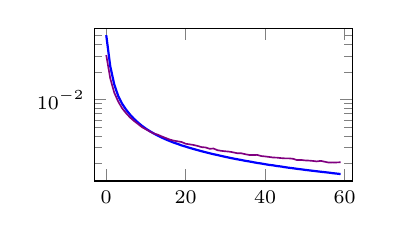
\begin{tikzpicture}

\definecolor{darkgray176}{RGB}{176,176,176}
\definecolor{darkorange25512714}{RGB}{255,127,14}
\definecolor{steelblue31119180}{RGB}{31,119,180}

\begin{axis}[speAE,
ymode=log,
ytick={0.0001,0.001,0.01,0.1,1},
yticklabels={
  \(\displaystyle {10^{-4}}\),
  \(\displaystyle {10^{-3}}\),
  \(\displaystyle {10^{-2}}\),
  \(\displaystyle {10^{-1}}\),
  \(\displaystyle {10^{0}}\)
}
]
\addplot [thick, blue]
table {%
0 0.0503827184438705
1 0.0231762751936913
2 0.014697564765811
3 0.0109478253871202
4 0.00899229943752289
5 0.00774224475026131
6 0.00684232404455543
7 0.00614844681695104
8 0.00560816191136837
9 0.00516596203669906
10 0.00480720214545727
11 0.00450789043679833
12 0.00425539258867502
13 0.00403159903362393
14 0.00384168932214379
15 0.00366993132047355
16 0.00352168921381235
17 0.00338485115207732
18 0.00327525730244815
19 0.00315655907616019
20 0.00306433159857988
21 0.00296860747039318
23 0.00280534545890987
24 0.00272952229715884
26 0.0025950912386179
27 0.00253195920959115
28 0.00247928220778704
29 0.00242134579457343
31 0.00231824209913611
33 0.00222833012230694
34 0.00218915846198797
35 0.00214463635347784
36 0.00211104960180819
38 0.00203325902111828
39 0.00200548488646746
40 0.00196877960115671
41 0.00193660240620375
42 0.00191451469436288
43 0.00188098242506385
44 0.00185941788367927
45 0.00182812963612378
46 0.00180087820626795
47 0.0017799154156819
48 0.00175378890708089
49 0.001733677694574
50 0.00170948228333145
54 0.00162926164921373
56 0.00159461738076061
57 0.00157220743130893
58 0.00155619683209807
59 0.00153788621537387
};
\addplot [semithick, violet]
table {%
0 0.0305683203041553
1 0.017071396112442
2 0.011926488019526
3 0.00952861737459898
4 0.0080207260325551
5 0.00709329778328538
6 0.00636689830571413
7 0.0058362390846014
8 0.00540540693327785
9 0.00499403430148959
11 0.0044674351811409
12 0.00425342144444585
13 0.00413477141410112
14 0.00395425315946341
16 0.00365695520304143
17 0.00355988088995218
18 0.0035015782341361
19 0.00343526271171868
20 0.0032912774477154
21 0.00324278487823904
22 0.00319049344398081
23 0.00311692943796515
24 0.00302586634643376
25 0.00299932225607336
26 0.00290136504918337
27 0.00292090233415365
28 0.00279996660538018
29 0.00275404471904039
30 0.00272374297492206
31 0.0027005102019757
32 0.00265146419405937
33 0.00259227468632162
34 0.00259035988710821
35 0.00253120018169284
36 0.00248397560790181
37 0.00248199491761625
38 0.0024878759868443
39 0.00241875112988055
40 0.00239369249902666
41 0.00236381567083299
42 0.00233046384528279
43 0.00232217158190906
44 0.00229623098857701
45 0.00228002434596419
46 0.00228015333414078
47 0.0022583685349673
48 0.00218693865463138
49 0.00219371449202299
50 0.00216764211654663
51 0.00215686019510031
52 0.00213886913843453
53 0.0021116673015058
54 0.00214252411387861
56 0.00205086614005268
57 0.00205984897911549
58 0.00205883500166237
59 0.00206905510276556
};
\end{axis}

\end{tikzpicture}

&
% This file was created with tikzplotlib v0.10.1.
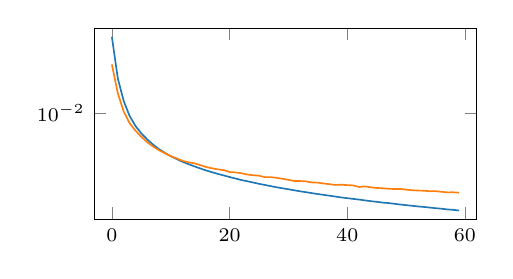
\begin{tikzpicture}

\definecolor{darkgray176}{RGB}{176,176,176}
\definecolor{darkorange25512714}{RGB}{255,127,14}
\definecolor{steelblue31119180}{RGB}{31,119,180}

\begin{axis}[compar,
	ymode=log]
\addplot [semithick, steelblue31119180]
table {%
0 0.0492035262286663
1 0.0207414887845516
2 0.0129387434571981
3 0.00945419538766146
4 0.00766767701134086
5 0.00656204577535391
6 0.00578529853373766
7 0.00518497824668884
8 0.00472294026985765
9 0.00436683231964707
10 0.00407265918329358
12 0.00362355192191899
14 0.00329436152242124
16 0.00302357808686793
18 0.0028144761454314
20 0.00263713044114411
22 0.00247619464062154
23 0.0024149629753083
25 0.00228715874254704
28 0.00212763133458793
30 0.00204079411923885
32 0.00195532198995352
35 0.00184639461804181
36 0.00181616784539074
37 0.00178282673005015
38 0.00175259064417332
39 0.00171963183674961
41 0.00166981155052781
42 0.00164510158356279
44 0.00159098510630429
45 0.00157107796985656
46 0.00154567917343229
47 0.00153023435268551
49 0.00148346740752459
50 0.00146513234358281
52 0.00142524391412735
53 0.00141107453964651
55 0.00137436343356967
56 0.00136018230114132
57 0.00134005874861032
58 0.00132755958475173
59 0.00130976806394756
};
\addplot [semithick, darkorange25512714]
table {%
0 0.0276999436318874
1 0.0152005106210709
2 0.0103711616247892
3 0.00814399775117636
4 0.00693845562636852
5 0.00611581327393651
6 0.00544816395267844
7 0.00498418230563402
8 0.00461689289659262
9 0.00433709705248475
10 0.0040805097669363
11 0.00389086711220443
12 0.00370007567107677
13 0.00358308735303581
14 0.00351104489527643
15 0.00338523765094578
16 0.00325000286102295
17 0.00316429394297302
18 0.00309449038468301
19 0.00304547790437937
20 0.00292374682612717
21 0.00290122651495039
22 0.00285399938002229
23 0.00277612800709903
24 0.00273615051992238
25 0.00271024717949331
26 0.00262898951768875
27 0.0026314384303987
28 0.00259054196067154
29 0.00254159467294812
30 0.00248572020791471
31 0.00242716423235834
32 0.00242336583323777
33 0.00240683532319963
34 0.0023516824003309
35 0.00234355125576258
36 0.00229976209811866
37 0.00226869224570692
38 0.00223404658026993
39 0.00224652979522943
40 0.00222630659118295
41 0.00221177469938993
42 0.00214156811125576
43 0.00216725165955722
44 0.00212531164288521
45 0.00209872331470251
46 0.0020835162140429
47 0.00206287042237818
48 0.0020514854695648
49 0.00205233367159963
50 0.00202494696713984
51 0.00200132979080081
52 0.00198752526193857
53 0.00198013707995415
54 0.00196109595708549
55 0.00196250132285058
57 0.00191261433064938
58 0.00191620655823499
59 0.00189937290269881
};
\end{axis}

\end{tikzpicture}


\\

\rotatebox[origin=lt]{90}{{\color{white}bbbb}PSNR}
& &
% This file was created with tikzplotlib v0.10.1.
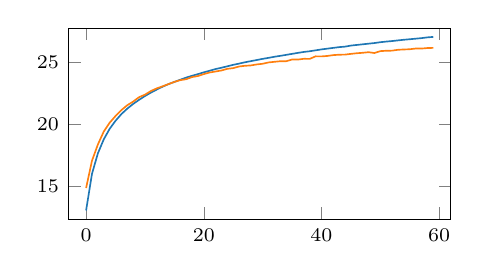
\begin{tikzpicture}

\definecolor{darkgray176}{RGB}{176,176,176}
\definecolor{darkorange25512714}{RGB}{255,127,14}
\definecolor{steelblue31119180}{RGB}{31,119,180}

\begin{axis}[compar]
\addplot [semithick, steelblue31119180]
table {%
0 12.9921646118164
1 15.9709796905518
2 17.6316299438477
3 18.7714214324951
4 19.6243877410889
5 20.2814331054688
6 20.825569152832
7 21.2693367004395
8 21.6509838104248
9 21.9818019866943
10 22.290246963501
11 22.5658435821533
12 22.8153610229492
13 23.0541896820068
14 23.2580280303955
15 23.4398918151855
17 23.7910099029541
18 23.9354858398438
19 24.0712852478027
20 24.2189025878906
21 24.3479061126709
22 24.4848308563232
23 24.5913696289062
25 24.826379776001
26 24.9274959564209
27 25.0352840423584
29 25.2175579071045
30 25.3115119934082
31 25.3935966491699
32 25.4829597473145
33 25.556453704834
36 25.7987403869629
37 25.8744373321533
38 25.9299793243408
40 26.0803718566895
43 26.2660179138184
44 26.3055362701416
45 26.3908996582031
48 26.5458984375
49 26.5972957611084
50 26.6657619476318
51 26.715425491333
52 26.7595901489258
54 26.8653030395508
55 26.9054412841797
57 26.9971542358398
58 27.0580635070801
59 27.0958271026611
};
\addplot [semithick, darkorange25512714]
table {%
0 14.8166589736938
1 17.0394096374512
2 18.3499698638916
3 19.4052104949951
4 20.12087059021
5 20.6666812896729
6 21.1473579406738
7 21.5459537506104
8 21.8410625457764
9 22.1983013153076
10 22.4017715454102
11 22.6959228515625
12 22.9133548736572
13 23.081262588501
15 23.4413452148438
16 23.5824241638184
17 23.658863067627
18 23.8318309783936
19 23.9167766571045
20 24.0732536315918
21 24.2038154602051
23 24.3677520751953
24 24.5024852752686
25 24.5585422515869
26 24.6924247741699
27 24.7486114501953
28 24.7782421112061
29 24.8595581054688
30 24.9125595092773
31 25.0220222473145
33 25.1214275360107
34 25.1195774078369
35 25.2583465576172
36 25.2555713653564
37 25.3172721862793
38 25.3094215393066
39 25.5182762145996
40 25.5110721588135
41 25.5484962463379
42 25.6167793273926
43 25.6492214202881
44 25.6571216583252
45 25.7165641784668
46 25.7686500549316
47 25.8048152923584
48 25.8545074462891
49 25.786994934082
50 25.9404563903809
51 25.9712791442871
52 25.9788265228271
53 26.0497512817383
54 26.0743026733398
55 26.0925235748291
56 26.1517753601074
57 26.1480541229248
58 26.1905174255371
59 26.2049503326416
};
\end{axis}

\end{tikzpicture}

&
% This file was created with tikzplotlib v0.10.1.
\begin{tikzpicture}

\definecolor{darkgray176}{RGB}{176,176,176}
\definecolor{darkorange25512714}{RGB}{255,127,14}
\definecolor{steelblue31119180}{RGB}{31,119,180}

\begin{axis}[speAE
]
\addplot [thick, blue]
table {%
0 13.141565322876
1 16.4121437072754
2 18.3559398651123
3 19.6229076385498
4 20.4739570617676
5 21.121940612793
6 21.6586933135986
7 22.1230201721191
8 22.5214576721191
9 22.8782615661621
10 23.190357208252
11 23.4693088531494
12 23.7187671661377
13 23.9537391662598
14 24.1627216339111
15 24.3614559173584
17 24.7117385864258
18 24.8552265167236
19 25.0149211883545
20 25.1446475982666
21 25.2817459106445
23 25.5281562805176
24 25.6464061737061
26 25.8652076721191
27 25.9728870391846
28 26.0626010894775
29 26.1668891906738
31 26.3553466796875
33 26.5267696380615
34 26.6037197113037
35 26.6926212310791
36 26.7621040344238
38 26.9245300292969
39 26.9842643737793
40 27.0646324157715
41 27.1359672546387
42 27.1858768463135
43 27.2623500823975
44 27.3123149871826
45 27.3857326507568
46 27.4515209197998
47 27.502025604248
48 27.5662307739258
49 27.6161918640137
50 27.6774291992188
54 27.8856678009033
56 27.9792156219482
57 28.0409603118896
58 28.0852375030518
59 28.1366901397705
};
\addplot [semithick, violet]
table {%
0 15.1579599380493
1 17.7009410858154
2 19.2677421569824
3 20.2477607727051
4 21.000602722168
5 21.5357780456543
6 22.0056056976318
7 22.3844528198242
8 22.7170639038086
9 23.0631332397461
11 23.5465240478516
12 23.761116027832
13 23.8813629150391
14 24.0759983062744
16 24.4174518585205
17 24.5327701568604
18 24.6020584106445
19 24.686107635498
20 24.8729763031006
22 25.0086402893066
23 25.1091575622559
24 25.2393856048584
25 25.2758560180664
26 25.4226875305176
27 25.3897819519043
28 25.5762500762939
29 25.6475467681885
30 25.6960620880127
31 25.7340679168701
32 25.8129272460938
33 25.9113426208496
34 25.9128532409668
35 26.0150375366211
36 26.0973606109619
37 26.0996189117432
38 26.0877342224121
39 26.2120475769043
40 26.2576656341553
41 26.3121719360352
42 26.3743019104004
43 26.388822555542
44 26.4381885528564
45 26.4681549072266
46 26.4669132232666
47 26.5092792510986
48 26.650764465332
49 26.6363906860352
50 26.6879081726074
51 26.709623336792
52 26.7456436157227
53 26.8024978637695
54 26.7362613677979
55 26.830005645752
56 26.9311370849609
57 26.9100170135498
58 26.911470413208
59 26.8904571533203
};
\end{axis}

\end{tikzpicture}

&
% This file was created with tikzplotlib v0.10.1.
\begin{tikzpicture}

\definecolor{darkgray176}{RGB}{176,176,176}
\definecolor{darkorange25512714}{RGB}{255,127,14}
\definecolor{steelblue31119180}{RGB}{31,119,180}

\begin{axis}[compar]
\addplot [semithick, steelblue31119180]
table {%
0 13.2728042602539
1 16.8960628509521
2 18.9158535003662
3 20.2616062164307
4 21.1672916412354
5 21.8417053222656
6 22.3864879608154
7 22.8624649047852
8 23.2667961120605
9 23.6068515777588
10 23.9097938537598
12 24.4168853759766
14 24.8300304412842
16 25.2024040222168
18 25.5130214691162
20 25.7950820922852
22 26.0686435699463
23 26.1776180267334
25 26.4130954742432
28 26.7272052764893
30 26.9088249206543
32 27.0939693450928
35 27.3428802490234
36 27.413818359375
39 27.651948928833
40 27.7185516357422
42 27.8439426422119
44 27.9892120361328
45 28.0439777374268
46 28.1142082214355
47 28.157564163208
49 28.2926139831543
50 28.3467178344727
52 28.4665489196777
53 28.5100154876709
55 28.6242618560791
56 28.6696815490723
57 28.73388671875
58 28.7748146057129
59 28.8332748413086
};
\addplot [semithick, darkorange25512714]
table {%
0 15.5871000289917
1 18.2080001831055
2 19.8783931732178
3 20.9324569702148
4 21.6307258605957
5 22.1794261932373
6 22.6829452514648
7 23.0694847106934
8 23.4025821685791
10 23.9384956359863
11 24.1459331512451
12 24.3642425537109
13 24.5037326812744
14 24.5904636383057
15 24.7491874694824
16 24.9271564483643
17 25.0406379699707
18 25.1383953094482
19 25.2085819244385
20 25.3868732452393
21 25.417516708374
22 25.4887542724609
23 25.6104412078857
24 25.6722221374512
25 25.7123947143555
26 25.8468799591064
27 25.840425491333
28 25.910120010376
29 25.9917697906494
30 26.0894184112549
31 26.1942081451416
32 26.1996917724609
33 26.2298202514648
34 26.3323268890381
35 26.3461246490479
36 26.4279403686523
37 26.4865188598633
38 26.5542278289795
39 26.528959274292
40 26.5687160491943
41 26.5965518951416
42 26.738151550293
43 26.6855964660645
44 26.7709846496582
45 26.8254051208496
46 26.8574275970459
47 26.9000606536865
48 26.9245586395264
49 26.922248840332
50 26.9806575775146
51 27.0315456390381
52 27.0615119934082
53 27.0784149169922
54 27.1207332611084
55 27.1165866851807
57 27.2284736633301
58 27.2209587097168
59 27.2595596313477
};
\end{axis}

\end{tikzpicture}

\end{tabular}
		\caption{Évolution de la MSE et du PSNR par batch des auto-encodeurs au cours des epochs. En bleu sur le set d'entraînement et en orange sur celui de test}
		\label{fig:AEperf}
	\end{figure}
	{\color{white}l}
	
	
	
	\subsection{Calcul pratique de \textit{F} et de son gradient}\label{anx:gradF}
	\quad
	
	\begin{enonce}[Notation]
		Comme $A$ est linéaire, dans toute la suite elle sera assimilé à matrice la représentant. Là où l'opérateur $A$ prend pour entrée un image $\bf{x}\in\R^{n\times m}$, sa représentation matricielle elle prend un vecteur $x\in\R^{nm}$. Par soucis de lisibilité on notera dans toute la suite les images sous forme de matrice en gras, leur version vectorielle en fin.
	\end{enonce}
	
	Le fait de supposer $A$ linéaire permet de calculer explicitement le gradient de $F$ à moindre coût :
	\begin{equation}\label{eq:gradient}
		\forall x\in\R^{nm},\qquad \nabla F(x)=\,^tA\big(Ax-y\big)
	\end{equation}{\color{white}l}
	Si la formule (\ref{eq:gradient}) est mathématiquement très simple, dès que $n$ et $m$ seront un peu trop grands, la taille de $A$ va très vite ralentir tout algorithme de descente et prendre énormément de place en mémoire.
	
	Pour éviter d'avoir à construire à explicitement on passe par la transformée de Fourier. On note $\F$ (resp. $\F^{-1}$) la matrice associée à la transformée (resp. inverse) de Fourier discrète. En notant de plus $\hat{\bf{x}}=\F \bf{x}$ et $\odot$ le produit terme à terme de vecteur/matrice, $A$ s'écrit alors :
	\begin{align*}\forall \bf{x}\in\R^{n\times m},\qquad A(\bf{x})=S\circ C_h(\bf{x})=S(\bf{h}*\bf{x})&=S\circ\F^{-1}\F(\bf{h}*\bf{x})\\
		&=S\circ\F^{-1}\big(\hat{\bf{h}}\odot\hat{\bf{x}}\big)\end{align*}
	\\
	Notons $D_h$ l'application/matrice associée au produit $\hat{h}\odot\cdot$. Comme la transformée de Fourier discrète et $D_h$ sont symétriques\footnote{comme $x$ a été aplatie, $\F$ n'est pas diagonale à proprement parler, nous y revenons plus loin}, le gradient de $F$ se réécrire comme :
	\begin{align*}\forall x\in\R^{nm},\qquad \nabla F(x)=\,^tA\big(Ax-y\big)&=\,^t\Big(S\F^{-1}D_h\F\Big)\big(S\F^{-1}D_h\F x-y\big)\\
		&=\,^t\F\,^tD_h\,^t\F^{-1}\,^tS\big(S\F^{-1}D_h\F x-y\big)\\
		&=\F D_h\F^{-1}\,^tS\big(S\F^{-1}D_h\F x-y\big)\end{align*}
	\\
	Sous cette forme et même s'il n'en n'a pas l'air, le gradient est bien plus simple à calculer et rapide à calculer.
	
	D'abord, la projection $S$ est très peu coûteuse en temps de calcul puisqu'elle consiste à ne garder qu'un certain nombre de pixel de l'image. Du point de vu python, il n'y a pas besoin de construire $S$, simplement de faire l'opération :
	\[\forall x\in\R^{n\times m},\qquad S(x):=\texttt{Sx = x[::n//p, ::m//q]}\]
	
	\noindent Inversement, la transposé $^tS$ à une image $y\in\R^{p\times q}$ revient à construire une image $^tSy=$\pyt{tSy} de taille $(n,m)$ remplie de 0 puis de faire la modification :
	\[\forall (i,j)\in\llbracket1,p\rrbracket\times\llbracket1,q\rrbracket,\qquad \texttt{tSy[i*n//p, j*p//q] = y[i,j]}\]{\color{white}l}
	
	Il n'y a pas besoin non plus de construire $D_h$, le produit $\hat{\bf{h}}\odot\hat{\bf{x}}$ suffit et le passage dans/hors de l'espace des fréquences est fait par \texttt{fft}. Ainsi, il n'y a jamais besoin d'aplatir les images et dans ce cas, on a bien la symétrie de $\F$ dans le sens où si, avec les conventions de notations d'Einstein,  $\hat{\bf{x}}^{kl}=\F_{ ij}^{kl}\bf{x}^{ij}$, alors $\F$ vérifie :
	\[\forall i,j,k,l,\qquad \F_{ij}^{kl}=\F_{kj}^{il}=\F_{il}^{kj}\]{\color{white}l}
	
	Enfin, comme son nom l'indique, il est plus naturel de construire le filtre \emph{passe-bas} directement dans l'espace de Fourier, et ce qui est fait dans le code. Les figures \textit{\ref{fig:passebas-g}} et \textit{\ref{fig:passebas-p}} montrent les applications successives de $A$ et $^tA$ à une image. La figure \textit{\ref{fig:passebas-p}} en particulier, met bien en évidence l'effet de Gibbs qui apparaît lorsque les fréquences sont brutalement coupées.
	\\
	\begin{figure}[H]\centering
		\begin{tabular}{l c c c l c c c l}
$x$ & & & & $Sx$ & & & & $^tS(Sx)$
\\

\includegraphics[width=0.25\textwidth]{resultats/compare_filter/seed21-x.png}
& & & &
\includegraphics[width=0.25\textwidth]{resultats/compare_filter/seed21-Ax-filtre=s.png}
& & & &
\includegraphics[width=0.25\textwidth]{resultats/compare_filter/seed21-tA(Ax)-filtre=s.png}\end{tabular}
		\caption{Application successive de $S$ et $^tS$ à une image}
		\label{fig:Sapplication}
	\end{figure}
	\vfill
	\begin{figure}[H]\centering
		\begin{tabular}{c c c c c c}

$\sigma=0.3$  &  $\sigma=0.4$  &  $\sigma=0.5$  &  $\sigma=0.6$  &  $\sigma=0.7$ & $\sigma=0.8$

\\

\includegraphics[width=0.14\textwidth]{resultats/compare_filter/seed21-f-filtre=g_param=0.3.png}
&
\includegraphics[width=0.14\textwidth]{resultats/compare_filter/seed21-f-filtre=g_param=0.4.png}
&
\includegraphics[width=0.14\textwidth]{resultats/compare_filter/seed21-f-filtre=g_param=0.5.png}
&
\includegraphics[width=0.14\textwidth]{resultats/compare_filter/seed21-f-filtre=g_param=0.6.png}
&
\includegraphics[width=0.14\textwidth]{resultats/compare_filter/seed21-f-filtre=g_param=0.7.png}
&
\includegraphics[width=0.14\textwidth]{resultats/compare_filter/seed21-f-filtre=g_param=0.8.png}

\\

\includegraphics[width=0.14\textwidth]{resultats/compare_filter/seed21-x.png}
&
\includegraphics[width=0.14\textwidth]{resultats/compare_filter/seed21-x.png}
&
\includegraphics[width=0.14\textwidth]{resultats/compare_filter/seed21-x.png}
&
\includegraphics[width=0.14\textwidth]{resultats/compare_filter/seed21-x.png}
&
\includegraphics[width=0.14\textwidth]{resultats/compare_filter/seed21-x.png}
&
\includegraphics[width=0.14\textwidth]{resultats/compare_filter/seed21-x.png}

\\

\includegraphics[width=0.14\textwidth]{resultats/compare_filter/seed21-Ax-filtre=g_param=0.3.png}
&
\includegraphics[width=0.14\textwidth]{resultats/compare_filter/seed21-Ax-filtre=g_param=0.4.png}
&
\includegraphics[width=0.14\textwidth]{resultats/compare_filter/seed21-Ax-filtre=g_param=0.5.png}
&
\includegraphics[width=0.14\textwidth]{resultats/compare_filter/seed21-Ax-filtre=g_param=0.6.png}
&
\includegraphics[width=0.14\textwidth]{resultats/compare_filter/seed21-Ax-filtre=g_param=0.7.png}
&
\includegraphics[width=0.14\textwidth]{resultats/compare_filter/seed21-Ax-filtre=g_param=0.8.png}

\\

\includegraphics[width=0.14\textwidth]{resultats/compare_filter/seed21-tA(Ax)-filtre=g_param=0.3.png}
&
\includegraphics[width=0.14\textwidth]{resultats/compare_filter/seed21-tA(Ax)-filtre=g_param=0.4.png}
&
\includegraphics[width=0.14\textwidth]{resultats/compare_filter/seed21-tA(Ax)-filtre=g_param=0.5.png}
&
\includegraphics[width=0.14\textwidth]{resultats/compare_filter/seed21-tA(Ax)-filtre=g_param=0.6.png}
&
\includegraphics[width=0.14\textwidth]{resultats/compare_filter/seed21-tA(Ax)-filtre=g_param=0.7.png}
&
\includegraphics[width=0.14\textwidth]{resultats/compare_filter/seed21-tA(Ax)-filtre=g_param=0.8.png}
\end{tabular}
		\caption{En première ligne la transformée de filtres  $\hat{\bf{h}}$ gaussien d'écart type $\sigma$, en deuxième l'image $\bf{x}$ avec en dessous le produits $A(\bf{x})$ puis $tA(A\bf{x})$.}
		\label{fig:passebas-g}
	\end{figure}
	\vfill
	\begin{figure}[H]\centering
		\begin{tabular}{c c c c c c}
$a=0.9$  &  $a=0.75$  &  $a=0.6$  &  $a=0.4$  &  $a=0.25$ & $a=0.1$

\\

\includegraphics[width=0.14\textwidth]{resultats/compare_filter/seed21-f-filtre=p_param=0.9.png}
&
\includegraphics[width=0.14\textwidth]{resultats/compare_filter/seed21-f-filtre=p_param=0.75.png}
&
\includegraphics[width=0.14\textwidth]{resultats/compare_filter/seed21-f-filtre=p_param=0.6.png}
&
\includegraphics[width=0.14\textwidth]{resultats/compare_filter/seed21-f-filtre=p_param=0.4.png}
&
\includegraphics[width=0.14\textwidth]{resultats/compare_filter/seed21-f-filtre=p_param=0.25.png}
&
\includegraphics[width=0.14\textwidth]{resultats/compare_filter/seed21-f-filtre=p_param=0.1.png}
\\ \\



\includegraphics[width=0.14\textwidth]{resultats/compare_filter/seed21-x.png}
&
\includegraphics[width=0.14\textwidth]{resultats/compare_filter/seed21-x.png}
&
\includegraphics[width=0.14\textwidth]{resultats/compare_filter/seed21-x.png}
&
\includegraphics[width=0.14\textwidth]{resultats/compare_filter/seed21-x.png}
&
\includegraphics[width=0.14\textwidth]{resultats/compare_filter/seed21-x.png}
&
\includegraphics[width=0.14\textwidth]{resultats/compare_filter/seed21-x.png}
\\ \\



\includegraphics[width=0.14\textwidth]{resultats/compare_filter/seed21-Ax-filtre=p_param=0.9.png}
&
\includegraphics[width=0.14\textwidth]{resultats/compare_filter/seed21-Ax-filtre=p_param=0.75.png}
&
\includegraphics[width=0.14\textwidth]{resultats/compare_filter/seed21-Ax-filtre=p_param=0.6.png}
&
\includegraphics[width=0.14\textwidth]{resultats/compare_filter/seed21-Ax-filtre=p_param=0.4.png}
&
\includegraphics[width=0.14\textwidth]{resultats/compare_filter/seed21-Ax-filtre=p_param=0.25.png}
&
\includegraphics[width=0.14\textwidth]{resultats/compare_filter/seed21-Ax-filtre=p_param=0.1.png}
\\ \\



\includegraphics[width=0.14\textwidth]{resultats/compare_filter/seed21-tA(Ax)-filtre=p_param=0.9.png}
&
\includegraphics[width=0.14\textwidth]{resultats/compare_filter/seed21-tA(Ax)-filtre=p_param=0.75.png}
&
\includegraphics[width=0.14\textwidth]{resultats/compare_filter/seed21-tA(Ax)-filtre=p_param=0.6.png}
&
\includegraphics[width=0.14\textwidth]{resultats/compare_filter/seed21-tA(Ax)-filtre=p_param=0.4.png}
&
\includegraphics[width=0.14\textwidth]{resultats/compare_filter/seed21-tA(Ax)-filtre=p_param=0.25.png}
&
\includegraphics[width=0.14\textwidth]{resultats/compare_filter/seed21-tA(Ax)-filtre=p_param=0.1.png}
\end{tabular}
		\caption{Idem avec cette fois $\hat{\bf{h}}$ qui est l'indicatrice de $[-a,a]\times[-a,a]$}
		\label{fig:passebas-p}
	\end{figure}
	
\end{annexe}



\newpage


\phantomsection
\addcontentsline{toc}{subsection}{Table des figures}
\listoffigures


\vspace{0.5cm}

\phantomsection
\addcontentsline{toc}{subsection}{Références}
\bibliography{zrefs}{}
\bibliographystyle{siam}


\end{document}